%%%%%%%%%%%%%%%%%%%%%%%%%%%%%%%%%%%%%%%%%%%%%%%%%%%%%%%%%%%%%%%%%%%%%%%%%%%%
%%% DOCUMENTCLASS %%%%%%%%%%%%%%%%%%%%%%%%%%%%%%%%%%%%%%%%%%%%%%%%%%%%%%%%%%
%%%%%%%%%%%%%%%%%%%%%%%%%%%%%%%%%%%%%%%%%%%%%%%%%%%%%%%%%%%%%%%%%%%%%%%%%%%%
\documentclass[
a4paper, % Stock and paper size.
12pt, % Type size.
% article,
% oneside, 
onecolumn, % Only one column of text on a page.
% openright, % Each chapter will start on a recto page.
% openleft, % Each chapter will start on a verso page.
openany, % A chapter may start on either a recto or verso page.
%oldfontcommands,
]{memoir}

% This file is a symbolic link to rayTemplate/latexCommon/PreambleMemoir
./../../rayTemplates/latexCommon/PreambleCommon.tex
./../../rayTemplates/latexCommon/PreambleMemoir.tex

%% Internal links
\hypersetup{
colorlinks=true,
linkcolor=blue,
filecolor=magenta,      
urlcolor=cyan,
citecolor=cyan,
%pdfborder={0 0 0},      % No borders around internal hyperlinks
pdftitle={RNO AlgoData},
pdfauthor={Ray White} % author
}
\urlstyle{same}

% Add bibtex files
\addbibresource{Bibliographies/library.bib}
\addbibresource{Bibliographies/website_ref.bib}


%%% THE DOCUMENT
%%% Where all the important stuff is included!
%%%-------------------------------------------------------------------------

\author{Raymon White}
\title{Ray's Notes On \\ 
       LeetCode\\
       (RNO-LeetCode)}


%%% NOTE: If re-compiling all, remember to comment out the silence warning
%%% at the top, for missing labels.

%\includeonly{Contents/ch08CmplTmPrgrmmng}

\begin{document}

%---------------------------------------------------------------------------
% Other settings
%---------------------------------------------------------------------------

% \numberwithin from the amsmath package provides per section numbering.
% we want per section. Note that the amsmath package is loaded from
% mathtools, loaded above.
% Note: we cannot put this in the preamble since lstlisting does not like
% it.
\numberwithin{equation}{chapter}
\numberwithin{figure}{chapter}
\numberwithin{lstlisting}{chapter}
\numberwithin{table}{chapter}

%%%%%%%%%%%%%%%%%%%%%%%%%%%%%%%%%%%%%%%%%%%%%%%%%%%%%%%%%%%%%%%%%%%%%%%%%%%%
%%%%%%%%%%%%%%%%%%%%%%%%%%%%%%%%%%%%%%%%%%%%%%%%%%%%%%%%%%%%%%%%%%%%%%%%%%%%

\frontmatter

\maketitle

\begin{abstract}
Insert abtract.

%Countless programmers have learned C++ from previous editions of C++ Primer
%.  During that time, C++ has matured greatly: Its focus, and that of its
%programming community, has widened from looking mostly at machine efficiency
%to devoting more attention to programmer efficiency.
%  
%In 2011, the C++ standards committee issued a major revision to the ISO C++
%standard. This revised standard is latest step in C++’s evolution and
%continues the emphasis on programmer efficiency. The primary goals of the
%new standard are to
%\begin{itemize}
%\item Make the language more uniform and easier to teach and to learn
%\item Make the standard libraries easier, safer, and more efficient to use
%\item Make it easier to write efficient abstractions and libraries
%\end{itemize}
%In this edition, we have completely revised the C++ Primer to use the latest
%standard. 
%
%%You can get an idea of how extensively the new standard has
%%affected C++ by reviewing the New Features Table of Contents, which lists
%%the sections that cover new material and appears on page xxi.
% 
%Some additions in the new standard, such as \ctt{auto} for type inference,
%are pervasive.  These facilities make the code in this edition easier to
%read and to understand.  Programs (and programmers!) can ignore type
%details, which makes it easier to concentrate on what the program is
%intended to do.  Other new features, such as smart pointers and move-enabled
%containers, let us write more sophisticated classes without having to
%contend with the intricacies of resource management. As a result, we can
%start to teach how to write your own classes much earlier in the book than
%we did in the Fourth Edition. We, and you, no longer have to worry about
%many of the details that stood in our way under the previous standard.
%
%
%Fully updated and recast for the newly released C++11 standard, this
%authoritative and comprehensive introduction to C++ will help you to learn
%the language fast, and to use it in modern, highly effective ways.
%Highlighting today's best practices, the authors show how to use both the
%core language and its standard library to write efficient, readable, and
%powerful code.
%
%C++ Primer, Fifth Edition, introduces the C++ standard library from the
%outset, drawing on its common functions and facilities to help you write
%useful programs without first having to master every language detail. The
%book's many examples have been revised to use the new language features and
%demonstrate how to make the best use of them. This book is a proven tutorial
%for those new to C++, an authoritative discussion of core C++ concepts and
%techniques, and a valuable resource for experienced programmers, especially
%those eager to see C++11 enhancements illuminated.
%
%Start Fast and Achieve More
%\begin{itemize}
%\item Learn how to use the new C++11 language features and the standard
%  library to build robust programs quickly, and get comfortable with
%  high-level programming
%
%\item Learn through examples that illuminate today’s best coding styles and
%  program design techniques
%
%\item Understand the ``rationale behind the rules'': why C++11 works as it
%  does
%
%\item Use the extensive crossreferences to help you connect related concepts
%  and insights
%
%\item Benefit from up-to-date learning aids and exercises that emphasize key
%  points, help you to avoid pitfalls, promote good practices, and reinforce
%  what you’ve learned
%\end{itemize}
%
%\noindent{}Access the source code for the extended examples from
%\url{informit.com/title/0321714113}

\end{abstract}
\clearpage

%\dominitoc% Initialization
\tableofcontents*

\listofalgorithms
\addtocontents{loa}{\def\string\figurename{Algorithm}}

\clearpage

\chapter[Introduction]
{Introduction
  \label{ch0introduction}}
\chaptermark{Introduction}

\section{Preface}

Some notes I've taken during LeetCode problems.

I will get latex warnings if I don't have at least one reference:
\cite{wiki_templatecpp}


%\lipsum[1-12]

\mainmatter

% NOTE: this is good for long Chapter names
%\chapter[medium-length title for TOC, if wanted]{full title name}
%\chaptermark{short title for running headers}

\chapter[Dynamic Programming]
{Dynamic Programming (DP)
  \label{chDynmcPrgrmmng}}
\chaptermark{Dynamic Programming}

When doing ``5. Longest Palindromic Substring'', I still have a bit of
problem with dynamic programming. So here are my own notes.


\section{Dynamic Programming---From Novice to Advanced
  \label{secDynmicPrgrmmngFrmNvcToAdvncd}}

\url{https://www.topcoder.com/community/data-science/data-science-tutorials/dynamic-programming-from-novice-to-advanced/}

By Dumitru---topcoder member

An important part of given problems can be solved with the help of dynamic
programming (\textbf{DP} for short). Being able to tackle problems of this
type would greatly increase your skill. I will try to help you in
understanding how to solve problems using DP. The article is based on
examples, because a raw theory is very hard to understand.

Note: If you're bored reading one section and you already know what's being
discussed in it---skip it and go to the next one.

\subsection{Introduction (Beginner)
  \label{subsecDPIntro}}

\rrheader{What is a dynamic programming, how can it be described?}

A \textbf{DP} is an algorithmic technique which is usually based on a
recurrent formula and one (or some) starting states. A sub-solution of the
problem is constructed from previously found ones \rrblue{(I think CLRS
  refers to states as structures. So we have to identity the optimal
  substructure which gives raise to the optimal solution. Thus, DP relies on
  the fact that an optimal solution can be constructed from optimal
  sub-solutions.)}. DP solutions have a polynomial complexity which assures
a much faster running time than other techniques like backtracking,
brute-force etc.

Now let's see the base of DP with the help of an example:

Given a list of $N$ coin \rrblue{(types)}, their values ($v_1$, $v_2$,
$\ldots$ , $v_N$), and the total sum $S$.  Find the minimum number of coins
the sum of which is $S$ (we can use as many coins of one type as we want),
or report that it's not possible to select coins in such a way that they sum
up to $S$.

Now let's start constructing a DP solution:

First of all we need to find a state for which an optimal solution is found
\rrblue{(i.e. the optimal sub-structure)} and with the help of which we can
find the optimal solution for the next state \rrblue{(so the optimal
  solution is created using the optimal sub-solution)}.

\rrheader{What does a ``state'' stand for?}

It's a way to describe a situation, a sub-solution for the problem. For
example a state would be the solution for sum $i$, where $i\leq S$
\rrblue{(i.e. a sub-structure which provides the optimal sub-solution for
  $i$, where $i\leq S$)}. A smaller state than state $i$ would be the
solution for any sum $j$, where $j<i$. For finding a state $i$, we need to
first \textbf{find all smaller states $\bm{j}$} ($j<i$) . Having found the
minimum number of coins which sum up to $i$, we can easily find the next
state---the solution for $i+1$.

\rrheader{How can we find it?}

It is simple---\rrhl{for each} coin $j$, with value $v_j\leq i$
\rrblue{(note that the value has to be less than $i$, since, e.g. we cannot
  create a sum $5p$ with a $10p$ coin)}, look at the minimum number of coins
found for the $i-v_j$ sum (we have already found it previously). Let this
number be $m$. If $m+1$ is less than the minimum number of coins already
found for current sum $i$, then we store this new result for it.
\rrblue{(This makes sense. See below.)}

\RayNotesBegin

Okay, this makes sense now (after I've seen the code). Now I will describe a
problem and how to solve it. The next section does more or less the same
thing but I think I can explain it better.

Say we have three coin types with values: $v = \brce*{v_1 = 1, v_2 = 3, v_3
  = 5}$, we want to minimize the number of coins required to make $S=11$.

First we have to think can we construct an optimal solution from an optimal
sub-solution? Say we have to solve for sum $i<S$, and we already obtained
the optimal sub-solutions for sums less than $i$. Then we simply work
through the coin types $\brce*{v_1..v_3}$ and say, if the solution to sum
$i$ contains coin $v_1$, what other coins should it contain? Well, $i - v_1
= k$ is the left over sum. So we look at the optimal value we've calculated
for $k$. Since we know we have used one coin already (in this case, $v_1$),
the solution would be the solution for $k$ plus $1$. And we keep doing this
with the rest of the coin types for this sum $i$, and update the most
optimal solution we've found so far.

Key take aways:
\begin{itemize}%[noitemsep,topsep=0pt]
\item Identified that we can create the solution to sum $i$ by using coin
  type $v_j$ (which gives us one coin) plus the solution obtained for sum
  $i-v_j$.
\item We work this out for all coin types $v_j$, and store/update the
  solution for $i$.
\item That's basically it. We're working from left to right of the sums:
  $0\leq i\leq S$, and at each step $i$, we know we've already calculated
  the optimal solution for $k<i$.
\end{itemize}

\RayNotesEnd

For a better understanding let's take this example \rrred{(yes, please do)}:
\begin{quotation}
Given coins with values $1$, $3$, and $5$.\\
And the sum $S$ is set to be $11$.
\end{quotation}

\begin{itemize}%[noitemsep,topsep=0pt]
\item First of all we note that for state 0 (sum $i=0$) we have found a
  solution with a minimum number of 0 coins.
\item \textbf{We then go to sum $\bm{i=1}$:}. First, we note that we haven't
  yet found a solution for this one (a value of $\infty$ would be a good
  sentinel, since we are trying to find the min. number of coins). 

  Now we work through the coins $j$. Then we see that only coin 1 is less
  than or equal to the current sum $i=1$.

  \begin{itemize}%[noitemsep,topsep=0pt]
  \item \textbf{Coin $j=1$, $v_1=1$:} Now we we see that for sum
    $i-v_1=1-1=0$, we have a solution with $0$ coins. Because we add one
    coin to this solution \rrblue{(since we used one coin of value $v_1 =
      1$)}, we'll have a solution with $1$ coin for sum $1$. It's the only
    solution yet found for this sum.  We write (save) it \rrblue{(in a table
      or something, so we can easily look up how many coins are needed to
      make value $i$)}.
  \end{itemize}
\item \textbf{Then we proceed to the next state---sum $\bm{i=2}$:}. We 
  again see that the only
  coin which is less or equal to this sum $i=2$ is the first coin, having a 
  value of $v_1 = 1$. So for each coin $j$:
  \begin{itemize}%[noitemsep,topsep=0pt]
  \item \textbf{Coin $j=1$, $v_1=1$:} The optimal solution found for sum
    $i-v_1=2-1=1$ is $1$ coin. This coin plus the first coin \rrblue{(the
      $v_1$ we just took off)} will sum up to $2$, and thus make a sum of
    $2$ with the help of only $2$ coins. This is the best and only solution
    for sum $i=2$.
  \end{itemize}
\item Now we proceed to sum $i=3$. We now have 2 coins which are to be
  analyzed---first $j=1$ \rrblue{(with value $v_1=1$)} and second one
  \rrblue{(with value $v_2=3$)}. Let's see the first one.
  \begin{itemize}%[noitemsep,topsep=0pt]
  \item \textbf{Coin $j=1$, $v_1=1$:} There exists a solution for sum
    $2=i-v_1=(3-1)$ and therefore we can construct from it a solution for
    sum $i=3$ by adding the first coin \rrblue{($j=1$ with $v_1=1$)} to it
    \rrblue{(``\emph{it}'' being the solution, so now the solution consists
      of one coin)}.  Because the best solution for sum $i=2$ that we found
    has $2$ coins, the new solution for sum $i=3$ will have $3$ coins
    \rrblue{(since the solution already has one coin)}.
  \item \textbf{Coin $j=2$, $v_1=3$:} Now let's take the second coin with
    value equal to $3$. The sum for which this coin needs to be added to
    make $i=3$ , is $i-v_2=3-3=0$. We know that sum $i=0$ is made up of $0$
    coins. Thus we can make a sum of $3$ with only one coin---$3$. We see
    that it's better than the previous found solution for sum $3$, which was
    composed of $3$ coins. We update it and mark it as having only $1$ coin.
  \end{itemize}
\item The same we do for sum $i=4$, and get a solution of $2$ coins ---
  $1+3$ \rrblue{(or $2+2$)}. And so on.
\end{itemize}

Pseudocode:
\begin{lstlisting}[style=pseudostyle]
Set Min[i] equal to Infinity for all of i
Min[0]=0

For i = 1 to S
  For j = 0 to N - 1
    If (Vj<=i AND Min[i-Vj]+1<Min[i])
      Then Min[i]=Min[i-Vj]+1

Output Min[S]
\end{lstlisting}

Here are the solutions found for all sums:

\begingroup
\renewcommand*{\arraystretch}{\arraystretchsize}
\begin{footnotesize}
\begin{longtable}{|l|p{2.5cm}|p{9cm}|}
% header and footer information
\hline
\endfirsthead
\hline
\endlastfoot
% body of table
Sum &Min. nr. of coins&Coin value added to a smaller sum to obtain his sum
(it is displayed in brackets)\\\hline
0&0&-\\\hline
1&1&1 (0)\\\hline
2&2&1 (1)\\\hline
3&1&3 (0)\\\hline
4&2&1 (3)\\\hline
5&1&5 (0)\\\hline
6&2&3 (3)\\\hline
7&3&1 (6)\\\hline
8&2&3 (5)\\\hline
9&3&1 (8)\\\hline
10&2&5 (5)\\\hline
11&3&1 (10)\\
\end{longtable}
\end{footnotesize}
\endgroup

Code for this is in:\\
\path{src/DynamicProgramming/rrrMinCoinSum.cpp}

As a result we have found a solution of 3 coins which sum up to 11.

Additionally, by tracking data about how we got to a certain sum from a
previous one, we can find what coins were used in building it. For example:
to sum $i=11$, we got by adding the coin with value 1 to a sum of $i=10$. To
sum $i=10$ we got from $5$. To $i=5$---from $0$. This way we find the coins
used: $1$, $5$ and $5$.

Having understood the basic way a DP is used, we may now see a slightly
different approach to it. It involves the change (update) of best solution
yet found for a sum $i$, whenever a better solution for this sum was found.
In this case the states aren't calculated consecutively. Let's consider the
problem above. Start with having a solution of $0$ coins for sum $0$. Now
let's try to add first coin (with value $1$) to all sums already found. If
the resulting sum $t$ will be composed of fewer coins than the one
previously found---we'll update the solution for it. Then we do the same
thing for the second coin, third coin, and so on for the rest of them. For
example, we first add coin with value $1$ to sum $0$ and get sum $1$.
Because we haven't yet found a possible way to make a sum of $1$---this is
the best solution yet found, and we store $S[1]=1$. By adding the same coin
to sum $1$, we'll get sum $2$, thus making $S[2]=2$. And so on for the first
coin. After the first coin is processed, take coin $2$ (having a value of
$3$) and consecutively try to add it to each of the sums already found.
Adding it to $0$, a sum $3$ made up of $1$ coin will result. Till now,
$S[3]$ has been equal to $3$, thus the new solution is better than the
previously found one. We update it and mark $S[3]=1$. After adding the same
coin to sum $1$, we'll get a sum $4$ composed of $2$ coins. Previously we
found a sum of $4$ composed of $4$ coins; having now found a better solution
we update $S[4]$ to $2$. The same thing is done for next sums---each time a
better solution is found, the results are updated.

\subsection{Elementary
  \label{subsecDPElementary}}

To this point, very simple examples have been discussed. Now let's see how
to find a way for passing from one state to another, for harder problems.
For that we will introduce a new term called \textbf{recurrent relation},
which makes a connection between a lower and a greater state.

Let's see how it works:

Given a sequence of $N$ numbers---$A[1],A[2],\ldots,A[N]$. Find the length
of the longest non-decreasing sequence.

As described above we must first find how to define a ``state'' \rrblue{(the
  structure)} which represents a sub-problem and thus we have to find a
solution for it. Note that in most cases the states rely on lower states and
are independent from greater states.

Let's define a state $i$ as being the longest non-decreasing sequence which
has its last number $A[i]$. This state carries only data about the length of
this sequence. Note that for $i<j$ the state $i$ is independent from $j$,
i.e.  doesn't change when we calculate state $j$. Let's see now how these
states are connected to each other. Having found the solutions for all
states lower than $i$, we may now look for state $i$. At first we initialize
it with a solution of $1$, which consists only of the $i$-th number itself.
Now for each $j<i$ let's see if it's possible to pass from it to state $i$.
This is possible only when $A[j]\leq A[i]$, thus keeping (assuring) the
sequence non-decreasing. So if $S[j]$ (the solution found for state $j$)
plus $1$ (number $A[i]$ added to this sequence which ends with number
$A[j]$) is better than a solution found for $i$ (i.e. $S[j]+1>S[i]$), we
make $S[i]=S[j]+1$. This way we consecutively find the best solutions for
each $i$, until last state $N$.

Let's see what happens for a randomly generated sequence: $\brce*{5, 3, 4,
  8, 6, 7}$:

\begingroup
\renewcommand*{\arraystretch}{\arraystretchsize}
\begin{footnotesize}
\begin{longtable}{|l|p{6cm}|p{6cm}|}
% header and footer information
\hline
\endfirsthead
\hline
\endlastfoot
% body of table
$i$&The length of the longest non-decreasing sequence of first $i$ numbers
&The last sequence $i$ from which we ``arrived'' to this one\\\hline
1&1&1 (first number itself)\\\hline
2&1&2 (second number itself)\\\hline
3&2&2\\\hline
4&3&3\\\hline
5&3&3\\\hline
6&4&5\\
\end{longtable}
\end{footnotesize}
\endgroup

%\rrred{\textbf{(Wow, this is so badly explained. I'll learn from
%    geeksforgeeks instead for now. I might come back to this later. So skip
%    to the geeksforgeeks section.)}}

\rrred{\textbf{\large (Wow, this is so badly explained. I'll learn from
    geeksforgeeks instead for now. I might come back to this later.)}}

%\rrheader{Practice problem:}
%
%Given an undirected graph G having N (1<N<=1000) vertices and positive
%weights. Find the shortest path from vertex 1 to vertex N, or state that
%such path doesn't exist.
%
%Hint: At each step, among the vertices which weren't yet checked and for
%which a path from vertex 1 was found, take the one which has the shortest
%path, from vertex 1 to it, yet found.
%
%Try to solve the following problems from topcoder competitions:
%\begin{itemize}%[noitemsep,topsep=0pt]
%\item 
%ZigZag---2003 TCCC Semifinals 3
%\item 
%BadNeighbors---2004 TCCC Round 4
%\item 
%FlowerGarden---2004 TCCC Round 1
%\end{itemize}
%
%\subsection{Intermediate
%  \label{subsecDPIntermediate}}
%
%Let's see now how to tackle bi-dimensional DP problems.
%
%\rrheader{Problem:}
%
%A table composed of N x M cells, each having a certain quantity of apples,
%is given. You start from the upper-left corner. At each step you can go down
%or right one cell. Find the maximum number of apples you can collect.
%
%This problem is solved in the same way as other DP problems; there is almost
%no difference.
%
%First of all we have to find a state. The first thing that must be observed
%is that there are at most 2 ways we can come to a cell---from the left (if
%it's not situated on the first column) and from the top (if it's not
%situated on the most upper row). Thus to find the best solution for that
%cell, we have to have already found the best solutions for all of the cells
%from which we can arrive to the current cell.
%
%From above, a recurrent relation can be easily obtained:\\
%S[i][j]=A[i][j] + max(S[i-1][j], if i>0 ; S[i][j-1], if j>0) (where i
%represents the row and j the column of the table , its left-upper corner
%having coordinates {0,0} ; and A[i][j] being the number of apples situated
%in cell i,j).
%
%S[i][j] must be calculated by going first from left to right in each row and
%process the rows from top to bottom, or by going first from top to bottom in
%each column and process the columns from left to right.
%
%Pseudocode:
%
%For i = 0 to N - 1
%   For j = 0 to M - 1
%   S[i][j] = A[i][j] +
%      max(S[i][j-1], if j>0 ; S[i-1][j], if i>0 ; 0)
%
%Output S[n-1][m-1]
%
%Here are a few problems, from topcoder Competitions, for practicing:
%
%AvoidRoads---2003 TCO Semifinals 4
%ChessMetric---2003 TCCC Round 4
%
%
%\subsection{Upper-Intermediate
%  \label{subsecDPUpperIntermediate}}
%
%This section will discuss about dealing DP problems which have an additional
%condition besides the values that must be calculated.
%
%As a good example would serve the following problem:
%
%Given an undirected graph G having positive weights and N vertices.
%
%You start with having a sum of M money. For passing through a vertex i, you
%must pay S[i] money. If you don't have enough money---you can't pass through
%that vertex. Find the shortest path from vertex 1 to vertex N, respecting
%the above conditions; or state that such path doesn't exist. If there exist
%more than one path having the same length, then output the cheapest one.
%Restrictions: 1<N<=100 ; 0<=M<=100 ; for each i, 0<=S[i]<=100. As we can
%see, this is the same as the classical Dijkstra problem (finding the
%shortest path between two vertices), with the exception that it has a
%condition. In the classical Dijkstra problem we would have used a
%uni-dimensional array Min[i] , which marks the length of the shortest path
%found to vertex i. However in this problem we should also keep information
%about the money we have. Thus it would be reasonable to extend the array to
%something like Min[i][j] , which represents the length of the shortest path
%found to vertex i, with j money being left. In this way the problem is
%reduced to the original path-finding algorithm. At each step we find the
%unmarked state (i,j) for which the shortest path was found. We mark it as
%visited (not to use it later), and for each of its neighbors we look if the
%shortest path to it may be improved. If so---then update it. We repeat this
%step until there will remain no unmarked state to which a path was found.
%The solution will be represented by Min[N-1][j] having the least value (and
%the greatest j possible among the states having the same value, i.e. the
%shortest paths to which has the same length).
%
%Pseudocode:
%
%Set states(i,j) as unvisited for all (i,j)
%Set Min[i][j] to Infinity for all (i,j)
%
%Min[0][M]=0
%
%While(TRUE)
%
%Among all unvisited states(i,j) find the one for which Min[i][j]
%is the smallest. Let this state found be (k,l).
%
%If there wasn't found any state (k,l) for which Min[k][l] is
%less than Infinity - exit While loop.
%
%Mark state(k,l) as visited
%
%For All Neighbors p of Vertex k.
%   If (l-S[p]>=0 AND
%    Min[p][l-S[p]]>Min[k][l]+Dist[k][p])
%      Then Min[p][l-S[p]]=Min[k][l]+Dist[k][p]
%   i.e.
%If for state(i,j) there are enough money left for
%going to vertex p (l-S[p] represents the money that
%will remain after passing to vertex p), and the
%shortest path found for state(p,l-S[p]) is bigger
%than [the shortest path found for
%state(k,l)] + [distance from vertex k to vertex p)],
%then set the shortest path for state(i,j) to be equal
%to this sum.
%End For
%
%End While
%
%Find the smallest number among Min[N-1][j] (for all j, 0<=j<=M);
%if there are more than one such states, then take the one with greater
%j. If there are no states(N-1,j) with value less than Infinity - then
%such a path doesn't exist.
%Here are a few TC problems for practicing:
%
%Jewelry---2003 TCO Online Round 4
%StripePainter---SRM 150 Div 1
%QuickSums---SRM 197 Div 2
%ShortPalindromes---SRM 165 Div 2
%
%
%
%\subsection{Advance
%  \label{subsecDPAdvance}}
%
%The following problems will need some good observations in order to reduce
%them to a dynamic solution.
%
%Problem StarAdventure---SRM 208 Div 1:
%
%Given a matrix with M rows and N columns (N x M). In each cell there's a
%number of apples.
%
%You start from the upper-left corner of the matrix. You can go down or right
%one cell. You need to arrive to the bottom-right corner. Then you need to go
%back to the upper-left cell by going each step one cell left or up. Having
%arrived at this upper-left cell, you need to go again back to the
%bottom-right cell.
%
%Find the maximum number of apples you can collect.
%When you pass through a cell---you collect all the apples left there.
%
%Restrictions: 1 < N, M <= 50 ; each cell contains between 0 and 1000 apples
%inclusive.
%
%First of all we observe that this problem resembles to the classical one
%(described in Section 3 of this article), in which you need to go only once
%from the top-left cell to the bottom-right one, collecting the maximum
%possible number of apples. It would be better to try to reduce the problem
%to this one. Take a good look into the statement of the problem---what can
%be reduced or modified in a certain way to make it possible to solve using
%DP? First observation is that we can consider the second path (going from
%bottom-right cell to the top-left cell) as a path which goes from top-left
%to bottom-right cell. It makes no difference, because a path passed from
%bottom to top, may be passed from top to bottom just in reverse order. In
%this way we get three paths going from top to bottom. This somehow decreases
%the difficulty of the problem. We can consider these 3 paths as left, middle
%and right. When 2 paths intersect (like in the figure below)
%
%
%we may consider them as in the following picture, without affecting the
%result:
%
%This way we'll get 3 paths, which we may consider as being one left, one
%middle and the other---right. More than that, we may see that for getting an
%optimal results they must not intersect (except in the leftmost upper corner
%and rightmost bottom corner). So for each row y (except first and last), the
%x coordinates of the lines (x1[y] , x2[y] and respectively x3[y] ) will be :
%x1[y] < x2[y] < x3[y] . Having done that---the DP solution now becomes much
%clearer. Let's consider the row y. Now suppose that for any configuration of
%x1[y-1] , x2[y-1] and x3[y-1] we have already found the paths which collect
%the maximum number of apples. From them we can find the optimal solution for
%row y. We now have to find only the way for passing from one row to the next
%one. Let Max[i][j][k] represent the maximum number of apples collected till
%row y-1 inclusive, with three paths finishing at column i, j, and
%respectively k. For the next row y, add to each Max[i][j][k] (obtained
%previously) the number of apples situated in cells (y,i) , (y,j) and (y,k).
%Thus we move down at each step. After we made such a move, we must consider
%that the paths may move in a row to the right. For keeping the paths out of
%an intersection, we must first consider the move to the right of the left
%path, after this of the middle path, and then of the right path. For a
%better understanding think about the move to the right of the left path –
%take every possible pair of, k (where j<k), and for each i (1 i<j) consider
%the move from position (i-1,j,k) to position (i,j,k). Having done this for
%the left path, start processing the middle one, which is done similarly; and
%then process the right path.
%
%
%
%TC problems for practicing:
%
%
%MiniPaint---SRM 178 Div 1
%
%\rrheader{Additional Note:}
%
%When have read the description of a problem and started to solve it, first
%look at its restrictions. If a polynomial-time algorithm should be
%developed, then it's possible that the solution may be of DP type. In this
%case try to see if there exist such states (sub-solutions) with the help of
%which the next states (sub-solutions) may be found. Having found that –
%think about how to pass from one state to another. If it seems to be a DP
%problem, but you can't define such states, then try to reduce the problem to
%another one (like in the example above, from Section 5).
%
%\rrheader{Mentioned in this writeup:}
%
%TCCC '03 Semifinals 3 Div I Easy---ZigZag
%TCCC '04 Round 4 Div I Easy---BadNeighbors
%TCCC '04 Round 1 Div I Med---FlowerGarden
%TCO '03 Semifinals 4 Div I Easy---AvoidRoads
%TCCC '03 Round 4 Div I Easy---ChessMetric
%TCO '03 Round 4 Div I Med---Jewelry
%SRM 150 Div I Med---StripePainter
%SRM 197 Div II Hard---QuickSums
%SRM 165 Div II Hard---ShortPalindromes
%SRM 208 Div I Hard---StarAdventure
%SRM 178 Div I Hard---MiniPaint
%More Resources
 
\section{geeksforgeeks: Dynamic Programming
  \label{secGFGDPMain}}

I'll be learning from: \url{http://www.geeksforgeeks.org/dynamic-programming/}

\section{Basic Concepts:}

\begin{itemize}%[noitemsep,topsep=0pt]
\item Overlapping Subproblems Property
\item Optimal Substructure Property
\item How to solve a Dynamic Programming Problem?
\item Tabulation vs Memoizatation
\end{itemize}

\section{Dynamic Programming | Set 1 (Overlapping Subproblems Property)
  \label{secGFGDPSet1OverlapSubprob}}

\textbf{Difficulty: 1.6}

Dynamic Programming is an algorithmic paradigm that solves a given complex
problem by breaking it into subproblems and stores the results of
subproblems to avoid computing the same results again. Following are the two
main properties of a problem that suggest that the given problem can be
solved using Dynamic programming.

In this post, we will discuss first property (Overlapping Subproblems) in
detail. The second property of Dynamic programming is discussed in next post
i.e. Set 2.

\begin{enumerate}[label=\textbf{\arabic*.}]
\item Overlapping Subproblems
\item Optimal Substructure
\end{enumerate}

\rrheader{1. Overlapping Subproblems:}

Like Divide and Conquer, Dynamic Programming combines solutions to
sub-problems. Dynamic Programming is mainly used when solutions of same
subproblems are needed again and again. In dynamic programming, computed
solutions to subproblems are stored in a table so that these don't have to
recomputed. So Dynamic Programming is not useful when there are no common
(overlapping) subproblems because there is no point storing the solutions if
they are not needed again. For example, Binary Search doesn't have common
subproblems. If we take example of following recursive program for Fibonacci
Numbers, there are many subproblems which are solved again and again.
\begin{lstlisting}[style=raycppnewsnippet]
/* simple recursive program for Fibonacci numbers */
int fib(int n)
{
  if ( n <= 1 )
    return n;
  return fib(n-1) + fib(n-2);
}
\end{lstlisting}

Recursion tree for execution of \ctt{fib(5)}:
\begin{lstlisting}[style=pseudostyle, numbers=none]
                              
                         fib(5)
                     /             \
               fib(4)                fib(3)
             /      \                /     \
         fib(3)      fib(2)         fib(2)    fib(1)
        /     \        /    \       /    \
  fib(2)   fib(1)  fib(1) fib(0) fib(1) fib(0)
  /    \
fib(1) fib(0)
\end{lstlisting}

We can see that the function \ctt{fib(3)} is being called 2 times. If we
would have stored the value of \ctt{fib(3)}, then instead of computing it
again, we could have reused the old stored value. There are following two
different ways to store the values so that these values can be reused:
\begin{enumerate}[label=\textbf{\alph*.}]
\item Memoization (Top Down)
\item Tabulation (Bottom Up)
\end{enumerate}

\textbf{a) Memoization (Top Down):} The memoized program for a problem is
similar to the recursive version with a small modification that it looks
into a lookup table before computing solutions. We initialize a lookup array
with all initial values as \textsc{nil}. Whenever we need solution to a
subproblem, we first look into the lookup table. If the precomputed value is
there then we return that value, otherwise we calculate the value and put
the result in lookup table so that it can be reused later.

Following is the memoized version for nth Fibonacci Number.
\begin{lstlisting}[style=raycppnewsnippet]
/* C/C++ program for Memoized version for nth Fibonacci number */
#include<stdio.h>
#define NIL -1
#define MAX 100
 
int lookup[MAX];
 
/* Function to initialize NIL values in lookup table */
void _initialize()
{
  int i;
  for (i = 0; i < MAX; i++)
    lookup[i] = NIL;
}
 
/* function for nth Fibonacci number */
int fib(int n)
{
  if (lookup[n] == NIL)
  {
    if (n <= 1)
      lookup[n] = n;
    else
      lookup[n] = fib(n-1) + fib(n-2);
  }
 
  return lookup[n];
}
 
int main ()
{
  int n = 40;
  _initialize();
  printf("Fibonacci number is %d ", fib(n));
  return 0;
}
\end{lstlisting}

\textbf{b) Tabulation (Bottom Up):} The tabulated program for a given
problem builds a table in bottom up fashion and returns the last entry from
table. For example, for the same Fibonacci number, we first calculate
\ctt{fib(0)} then \ctt{fib(1)} then \ctt{fib(2)} then \ctt{fib(3)} and so
on. So literally, we are building the solutions of subproblems bottom-up.

Following is the tabulated version for nth Fibonacci Number.
\begin{lstlisting}[style=raycppnewsnippet]
/* C program for Tabulated version */
#include<stdio.h>
int fib(int n)
{
  int f[n+1];
  int i;
  f[0] = 0;   f[1] = 1; 
  for (i = 2; i <= n; i++)
      f[i] = f[i-1] + f[i-2];
 
  return f[n];
}
  
int main ()
{
  int n = 9;
  printf("Fibonacci number is %d ", fib(n));
  return 0;
}
\end{lstlisting}
Output:
\begin{lstlisting}[style=rayio]
Fibonacci number is 34 
\end{lstlisting}

Both Tabulated and Memoized store the solutions of subproblems. In Memoized
version, table is filled on demand while in Tabulated version, starting from
the first entry, all entries are filled one by one. Unlike the Tabulated
version, all entries of the lookup table are not necessarily filled in
Memoized version. For example, Memoized
solution\footnote{\url{https://www.ics.uci.edu/~eppstein/161/960229.html}}
of the LCS
problem\footnote{\url{https://en.wikipedia.org/wiki/Longest\_common\_subsequence\_problem}}
doesn't necessarily fill all entries.

To see the optimization achieved by Memoized and Tabulated solutions over
the basic Recursive solution, see the time taken by following runs for
calculating 40th Fibonacci number \rrblue{(do this as an exercise)}:
\begin{itemize}%[noitemsep,topsep=0pt]
\item Recursive solution
\item Memoized solution
\item Tabulated solution
\end{itemize}

Time taken by Recursion method is much more than the two Dynamic Programming
techniques mentioned above---Memoization and Tabulation!

Also see method 2 of Ugly
Number\footnote{http://www.geeksforgeeks.org/?p=753} post for one more
simple example where we have overlapping subproblems and we store the
results of subproblems.

We will be covering Optimal Substructure Property and some more example
problems in future posts on Dynamic Programming.

Try following questions as an exercise of this post.
\begin{enumerate}[label=\textbf{\arabic*.}]
\item Write a Memoized solution for LCS problem. Note that the Tabular
  solution is given in the CLRS book.
\item How would you choose between Memoization and Tabulation?
\end{enumerate}


%%%%%%%%%%%%%%%%%%%%%%%%%%%%%%%%%%%%%%%%%%%%%%%%%%%%%%%%%%%%%%%%%%%%%%%%%%%%
%%%%%%%%%%%%%%%%%%%%%%%%%%%%%%%%%%%%%%%%%%%%%%%%%%%%%%%%%%%%%%%%%%%%%%%%%%%%
%%%%%%%%%%%%%%%%%%%%%%%%%%%%%%%%%%%%%%%%%%%%%%%%%%%%%%%%%%%%%%%%%%%%%%%%%%%%

\section{Dynamic Programming | Set 2 (Optimal Substructure Property)
  \label{secGFGDPSet2OptimalSubstruct}}

\textbf{Difficulty: 1.7}

As we discussed in Set 1, following are the two main properties of a problem
that suggest that the given problem can be solved using Dynamic programming:
\begin{enumerate}[label=\textbf{\arabic*.}]
\item Overlapping Subproblems
\item Optimal Substructure
\end{enumerate}

We have already discussed Overlapping Subproblem property in the Set 1. Let
us discuss Optimal Substructure property here.

\textbf{2) Optimal Substructure:} A given problems has Optimal Substructure
Property if optimal solution of the given problem can be obtained by using
optimal solutions of its subproblems.

For example, the Shortest Path problem has following optimal substructure
property:

If a node $x$ lies in the shortest path from a source node $u$ to
destination node $v$ then the shortest path from $u$ to $v$ is combination
of shortest path from $u$ to $x$ and shortest path from $x$ to $v$. The
standard All Pair Shortest Path algorithms like
Floyd-Warshall\footnote{\url{https://en.wikipedia.org/wiki/Floyd\%E2\%80\%93Warshall\_algorithm}}
and
Bellman-Ford\footnote{\url{https://en.wikipedia.org/wiki/Bellman\%E2\%80\%93Ford\_algorithm}}
are typical examples of Dynamic Programming.

On the other hand, the Longest Path problem doesn't have the Optimal
Substructure property. Here by Longest Path we mean longest simple path
(path without cycle) between two nodes. Consider the following unweighted
graph given in the CLRS book. 

\begin{figure}
\centering
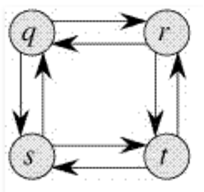
\includegraphics[width=0.2\textwidth]{Images/DPLongestPath}
\label{DPLongestPath}
\end{figure}

There are two longest paths from $q$ to $t$:
$q\to r\to t$ and $q\to s\to t$. Unlike shortest paths, these longest paths
do not have the optimal substructure property. For example, the longest path
$q\to r\to t$ is not a combination of longest path from $q$ to $r$ and
longest path from $r$ to $t$, because the longest path from $q$ to $r$ is
$q\to s\to t\to r$ and the longest path from $r$ to $t$ is $r\to q\to s\to
t$.

\section{How to solve a Dynamic Programming Problem?
  \label{secGFGDPHowToSolve}}

\textbf{Difficulty: 3.4}

\textbf{D}ynamic \textbf{P}rogramming (DP) is a technique that solves some
particular type of problems in \rrhl{Polynomial Time}. Dynamic Programming
solutions are faster than exponential brute method and can be easily proved
for their correctness.  Before we study how to think Dynamically for a
problem, we need to learn:
\begin{enumerate}[label=\textbf{\arabic*.}]
\item Overlapping Subproblems
\item Optimal Substructure Property
\end{enumerate}

\textbf{Steps to solve a DP}
\begin{enumerate}[label=\textbf{\arabic*.}]
\item Identify if it is a DP problem
\item Decide a state expression with least parameters
\item Formulate state relationship    
\item Do tabulation (or add memoization)
\end{enumerate}

\rrheader{Step 1 : How to classify a problem as a Dynamic Programming
  Problem?}

\begin{itemize}%[noitemsep,topsep=0pt]
\item Typically, \rrhl{all the problems that require to maximize or minimize
    certain quantity or counting problems that say to count the arrangements
    under certain condition or certain probability problems can be solved by
    using Dynamic Programming.}
\item \rrhl{All dynamic programming problems} satisfy the \rrhl{overlapping
    subproblems property} and \rrhl{most of the classic dynamic problems}
  also satisfy the \rrhl{optimal substructure property}. Once, we observe
  these properties in a given problem, be sure that it can be solved using
  DP.
\end{itemize}

\rrheader{Step 2 : Deciding the state}

DP problems are all about state and their transition. This is the most basic
step which must be done very carefully because the state transition depends
on the choice of state definition you make. So, let's see what do we mean by
the term ``state''.

\rrhl{State:} A state can be defined as the set of parameters that can
uniquely identify a certain position or standing in the given problem. This
set of parameters should be as small as possible to reduce state space.

For example: In our famous Knapsack
problem\footnote{\url{http://www.geeksforgeeks.org/knapsack-problem/}}, we
define our state by two parameters \textbf{index} and \textbf{weight} i.e
\ctt{DP[index][weight]}.  Here \ctt{DP[index][weight]} tells us the maximum
profit it can make by taking items from range $0$ to $index$ having the
capacity of sack to be weight.  Therefore, here the parameters index and
weight together can uniquely identify a subproblem for the knapsack problem.

So, our first step will be deciding a state for the problem after
identifying that the problem is a DP problem.

As we know DP is all about using calculated results to formulate the final
result.

So, our next step will be to find a relation between previous states to
reach the current state.

\rrheader{Step 3 : Formulating a relation among the states}

This part is the hardest part of for solving a DP problem and requires a
lots of intuition, observation and practice. Let's understand it by
considering a sample problem

\begin{mdframed}[style=mdfNOTE]

Given $3$ numbers $\brce*{1,3,5}$, we need to tell the total number of ways
we can form a number '$N$' using the sum of the given three numbers.
(allowing repetitions and different arrangements).

Total number of ways to form $6$ is : $8$\\
$1+1+1+1+1+1$\\
$1+1+1+3$\\
$1+1+3+1$\\
$1+3+1+1$\\
$3+1+1+1$\\
$3+3$\\
$1+5$\\
$5+1$\\

\end{mdframed}

Let's think dynamically for this problem. So, first of all, we decide a
state for the given problem. We will take a parameter $n$ to decide state as
it can uniquely identify any subproblem. So, our state dp will look like
state($n$). Here, state($n$) means the total number of arrangements to form
n by using $\brce*{1,3,5}$ as elements.

Now, we need to compute state($n$).

\rrheader{How to do it?}

So here the intuition comes into action. As we can only use $1$, $3$ or $5$
to form a given number. Let us assume that we know the result for
$n=1,2,3,4,5,6$; being termilogistic let us say we know the result for the
state($n=1$), state($n=2$), state($n=3$)$, \ldots, $ state($n=6$).

Now, we wish to know the result of the state($n=7$). See, we can only add
$1$, $3$ and $5$. Now we can get a sum total of $7$ by the following 3 ways:

\textbf{1) Adding 1 to all possible combinations of state($\textbf{n=6}$)}
E.g.:\\
$[ (1+1+1+1+1+1) + 1]$\\
$[ (1+1+1+3) + 1]$\\
$[ (1+1+3+1) + 1]$\\
$[ (1+3+1+1) + 1]$\\
$[ (3+1+1+1) + 1]$\\
$[ (3+3) + 1]$\\
$[ (1+5) + 1]$\\
$[ (5+1) + 1]$\\

\textbf{2) Adding 3 to all possible combinations of state($\bm{n=4}$)}

E.g.:\\
$[(1+1+1+1) + 3]$\\
$[(1+3) + 3]$\\
$[(3+1) + 3]$\\

\textbf{3) Adding 5 to all possible combinations of state($\bm{n=2}$)}

E.g.:\\
$[ (1+1) + 5]$

Now, think carefully and satisfy yourself that the above three cases are
covering all possible ways to form a sum total of $7$. \rrblue{(Yup, it's
  exhaustive.)}

Therefore, we can say that result for\\
state($7$) = state($6$) + state($4$) + state($2$)\\
or\\
state($7$) = state($7-1$) + state($7-3$) + state($7-5$)

In general,\\
\textbf{state($\bm{n}$) = state($\bm{n-1}$) + state($\bm{n-3}$) +
  state($\bm{n-5}$)}\\

So, our code will look like:
\begin{lstlisting}[style=raycppnewsnippet]
// Returns the number of arrangements to 
// form 'n' 
int solve(int n)
{ 
  // base case
  if (n < 0) 
    return 0;
  if (n == 0)  
    return 1;  
 
  return solve(n-1) + solve(n-3) + solve(n-5);
} 
\end{lstlisting}
The above code seems exponential as it is calculating the same state again
and again. So, we just need to add a memoization.

\rrheader{Step 4 : Adding memoization or tabulation for the state}

This is the easiest part of a dynamic programming solution. We just need to
store the state answer so that next time that state is required, we can
directly use it from our memory

Adding memoization to the above code
\begin{lstlisting}[style=raycppnewsnippet]
// initialize to -1
int dp[MAXN];
 
// this function returns the number of 
// arrangements to form 'n' 
int solve(int n)
{ 
  // base case
  if (n < 0)  
    return 0;
  if (n == 0)  
    return 1;
 
  // checking if already calculated
  if (dp[n]!=-1) 
      return dp[n];
 
  // storing the result and returning
  return dp[n] = solve(n-1) + solve(n-3) + solve(n-5);
}
\end{lstlisting}

Another way is to add tabulation and make solution iterative. Please refer
tabulation and
memoization\footnote{\url{http://www.geeksforgeeks.org/tabulation-vs-memoizatation/}}
for more details.

Dynamic Programming comes with a lots of practice. One must try solving
various classic DP problems that can be found
here\footnote{\url{http://www.geeksforgeeks.org/fundamentals-of-algorithms/#DynamicProgramming}}.
You may check the below problems first and try solving them using the above
described steps:-
\begin{itemize}%[noitemsep,topsep=0pt]
\item \url{http://www.spoj.com/problems/COINS/}
\item \url{http://www.spoj.com/problems/ACODE/}
\item
  \url{http://www.geeksforgeeks.org/dynamic-programming-set-6-min-cost-path/}
\item 
  \url{http://www.geeksforgeeks.org/dynamic-programming-subset-sum-problem/}
\item
  \url{http://www.geeksforgeeks.org/dynamic-programming-set-7-coin-change/}
\item
  \url{http://www.geeksforgeeks.org/dynamic-programming-set-5-edit-distance/}
\end{itemize}


%%%%%%%%%%%%%%%%%%%%%%%%%%%%%%%%%%%%%%%%%%%%%%%%%%%%%%%%%%%%%%%%%%%%%%%%%%%%
%%%%%%%%%%%%%%%%%%%%%%%%%%%%%%%%%%%%%%%%%%%%%%%%%%%%%%%%%%%%%%%%%%%%%%%%%%%%
%%%%%%%%%%%%%%%%%%%%%%%%%%%%%%%%%%%%%%%%%%%%%%%%%%%%%%%%%%%%%%%%%%%%%%%%%%%%

\section{Tabulation vs Memoizatation
  \label{secGFGDPTabVsMemo}}

\textbf{Difficulty: 2.7}

There are following two different ways to store the values so that the
values of a problem can be reused. Here, will discuss two patterns of
solving DP problem:
\begin{enumerate}[label=\textbf{\arabic*.}]
\item Tabulation: Bottom Up
\item Memoization: Top Down
\end{enumerate}
Before getting to the definitions of the above two terms consider the below
statements:
\begin{itemize}%[noitemsep,topsep=0pt]
\item \textbf{Version 1:} I will study the theory of Dynamic Programming
  from GeeksforGeeks, then I will practice some problems on classic DP and
  hence I will master Dynamic Programming.
\item \textbf{Version 2:} To Master Dynamic Programming, I would have to
  practice Dynamic problems and to practice problems---Firstly, I would have
  to study some theory of Dynamic Programming from GeeksforGeeks
\end{itemize}
Both the above versions say the same thing, just the difference lies in the
way of conveying the message and that's exactly what Bottom Up and Top Down
DP do. \textbf{Version 1} can be related to as Bottom Up DP and
\textbf{Version 2} can be related as Top Down DP.

\rrheader{Tabulation Method---Bottom Up Dynamic Programming}

As the name itself suggests starting from the bottom and cumulating answers
to the top. Let's discuss in terms of state transition.

Let's describe a state for our DP problem to be $dp[x]$ with $dp[0]$ as
base state and $dp[n]$ as our destination state. So, we need to find the
value of destination state i.e $dp[n]$.

If we start our transition from our base state i.e $dp[0]$ and follow our
state transition relation to reach our destination state $dp[n]$, we call it
\textbf{Bottom Up approach} as it is quite clear that we started our
transition from the bottom base state and reached the top most desired
state.

\rrheader{Now, Why do we call it tabulation method?}

To know this, let's first write some code to calculate the factorial of a
number using bottom up approach. Once, again as our general procedure to
solve a DP, we first define a state. In this case, we define a state as
$dp[x]$, where $dp[x]$ is to find  the factorial of $x$.

Now, it is quite obvious that $dp[x+1] = dp[x]\times (x+1)$
\begin{lstlisting}[style=raycppnewsnippet]
// Tabulated version to find factorial x.
int dp[MAXN];

// base case
int dp[0] = 1; // 0! = 1
for (int i = 1; i<=n; i++)
{
  dp[i] = dp[i-1] * i;
}
\end{lstlisting}
The above code clearly follows the bottom up approach as it starts its
transition from the bottom most base case $dp[0]$ and reaches it destination
state $dp[n]$. Here, we may notice that the $dp$ table is being populated
sequentially and we are \textbf{directly accessing the calculated states
  from the table itself} and hence, we call it tabulation method.

\rrheader{Memoization Method---Top Down Dynamic Programming}

Once, again let's describe it in terms of state transition. If we need to
find the value for some state say $dp[n]$ and instead of starting from the
base state, i.e. $dp[0]$, we ask our answer from the states that can be
reached from the destination state $dp[n]$, following the state transition
relation, then it is the top-down fashion of DP.

Here, we start our journey from the top most destination state and compute
its answer by taking in count the values of states that can reach the
destination state, till we reach the bottom most base state.

Once again, let's write the code for the factorial problem in top down
fashion
\begin{lstlisting}[style=raycppnewsnippet]
// Memoized version to find factorial x.
// To speed up we store the values
// of calculated states

// initialized to -1
int dp[MAXN]

// return fact x!
int solve(int x)
{
    if (x==0)
        return 1;
    if (dp[x]!=-1)
        return dp[x];
    return (dp[x] = x * solve(x-1));
}
\end{lstlisting}
As we can see we are storing the most recent cache up to a limit so that if
next time we got a call for the same state we simply return it from the
memory. So, this is why we call it memoization as we are storing the most
recent state values.

In this case the memory layout is linear that's why it may seem that the
memory is being filled in a sequential manner like the tabulation method,
but you may consider any other top down DP having 2D memory layout like Min
Cost
Path\footnote{http://www.geeksforgeeks.org/dynamic-programming-set-6-min-cost-path/},
here the memory is not filled in a sequential manner.

\begingroup
\renewcommand*{\arraystretch}{\arraystretchsize}
\begin{footnotesize}
\begin{longtable}{|p{2.5cm}|p{5.5cm}|p{5.5cm}|}
% header and footer information
\hline
\endfirsthead
\hline
\endlastfoot
% body of table
    &\textbf{Tabulation}&\textbf{Memoization}\\\hline
\textbf{State}&State Transition relation is difficult to think&State
transition relation is easy to think\\\hline
\textbf{Code} &Code gets complicated when lot of conditions are
required&Code is easy and less complicated\\\hline
\textbf{Speed}&Fast, as we directly access previous states from the
table&Slow due to a lot of recursive calls and return statements\\\hline
\textbf{Subproblem solving}&If all subproblems must be solved at least once,
bottom-up dynamic-programming algorithm usually outperforms a top-down
memoized algorithm by a constant factor.&If \textbf{\emph{some}} subproblem
in the subproblem space need not be solved at all, the memoized solution has
the advantage of solving only those subproblems that are definitely
required\\\hline
\textbf{Table Entries}&In the tabulated version, starting from the first
entry, all entries are filled on by one.& Unlike the tabulated version, all
entries of the lookup table re not necessarily filled in memoized version.
The table is filled on demand.
\end{longtable}
\end{footnotesize}
\endgroup


%%%%%%%%%%%%%%%%%%%%%%%%%%%%%%%%%%%%%%%%%%%%%%%%%%%%%%%%%%%%%%%%%%%%%%%%%%%%
%%%%%%%%%%%%%%%%%%%%%%%%%%%%%%%%%%%%%%%%%%%%%%%%%%%%%%%%%%%%%%%%%%%%%%%%%%%%
%%%%%%%%%%%%%%%%%%%%%%%%%%%%%%%%%%%%%%%%%%%%%%%%%%%%%%%%%%%%%%%%%%%%%%%%%%%%

\section{Dynamic Programming | Set 3 (Longest Increasing Subsequence)
  \label{secGFGDPSet3LIS}}

\url{http://www.geeksforgeeks.org/longest-increasing-subsequence/}

\textbf{Difficulty: 3.1}

Let us discuss Longest Increasing Subsequence (LIS) problem as an example
problem that can be solved using Dynamic Programming.

The Longest Increasing Subsequence (LIS) problem is to find the length of
the longest subsequence of a given sequence such that all elements of the
subsequence are sorted in increasing order. For example, the length of LIS
for $\brce*{10, 22, 9, 33, 21, 50, 41, 60, 80}$ is $6$ and LIS is
$\brce*{10, 22, 33, 50, 60, 80}$.

\begin{center}
\begin{tabular}{|c|c|c|c|c|c|c|c|c|c|}
\hline
\ctt{arr[]}&10&22&9&33&21&50&41&60&80\\\hline
LIS&1&2& &3& &4& &5&6\\ 
\hline
\end{tabular}
\end{center}

\begin{mdframed}[style=mdfNOTE,
frametitle={More examples}]

\begin{lstlisting}[style=raygeneric]
Input  : arr[] = {3, 10, 2, 1, 20}
Output : Length of LIS = 3
The longest increasing subsequence is 3, 10, 20

Input  : arr[] = {3, 2}
Output : Length of LIS = 1
The longest increasing subsequences are {3} and {2}

Input  : arr[] = {50, 3, 10, 7, 40, 80}
Output : Length of LIS = 4
The longest increasing subsequence is {3, 7, 40, 80}
\end{lstlisting}

\end{mdframed}

\RayNotesBegin

Oh, this was the longest increasing subsequence of the ``elementary''
section earlier. This is so much clearer with more examples.

Let's try to remember what we have to do:
\begin{enumerate}[label=\textbf{\arabic*.}]
\item \textbf{Identify if it is a DP problem:} For this to be a DP problem,
  \textbf{(1)} we need to identify a recursive solution which exhibits
  optimal substructure, by this I mean that the optimal solution is formed
  by optimal solutions to subproblems. \textbf{(2)} We also need overlapping
  subproblems. This is normally done by constructing the recursion tree for
  a particular set of input and seeing if there are repeated subproblems.
\item \textbf{Decide on a state expression with least parameters:} The state
  can be \textsc{lis}$[i]$, which is the longest increasing subsequence
  ending at $i$. E.g.

\begin{tabular}{|c|c|c|c|c|c|c|}
\hline
\ctt{arr[]}&8&9&6&7&4&5\\\hline
\ctt{lis[]}&1&2&1&2&1&2\\ 
\hline
\end{tabular}

\noindent{}Output : Length of $\textsc{lis}=2$\\
The longst incr. subseq. is: 8, 9 (select first one)\\
\textit{How did I get the \ctt{lis[]} values? Work through the \ctt{arr[]}
  values and for each one, count the length of the longest increasing
  subsequence ending \textbf{here}. So for $8$, clearly the \textsc{lis} is
  $1$. Next look at $9$, clearly the \textsc{lis} ending there is $2$. For
  $6$, there are no previous values in \ctt{arr} that can contribute to the
  \textsc{lis} ending here, so it's $\textsc{lis}=1$.}\\

\begin{tabular}{|c|c|c|c|c|c|c|}
\hline
\ctt{arr[]}&4&5&9&8&6&7\\\hline
\ctt{lis[]}&1&2&3&3&3&4\\ 
\hline
\end{tabular}

\noindent{}Output : Length of $\textsc{lis}=4$\\
The longst incr. subseq. is: $\brce*{4,5,6,7}$\\

\begin{tabular}{|c|c|c|c|c|c|c|c|c|c|}
\hline
\ctt{arr[]}&10&22&9&33&21&50&41&60&80\\\hline
\ctt{lis[]}& 1& 2&1& 3& 2& 4& 4& 5& 6\\ 
\hline
\end{tabular}

\noindent{}Output : Length of $\textsc{lis}=6$\\
The longst incr. subseq. is: $\brce*{10,22,33,50 (41),60,80}$\\

\begin{tabular}{|c|c|c|c|c|c|c|c|c|c|}
\hline
\ctt{arr[]}&3&10&2&1&20\\\hline
\ctt{lis[]}&1& 2&1&1&3\\ 
\hline
\end{tabular}

\noindent{}Output : Length of $\textsc{lis}=3$\\
The longst incr. subseq. is: $\brce*{3,10,20}$\\

\begin{tabular}{|c|c|c|c|c|c|c|c|c|c|}
\hline
\ctt{arr[]}&3&2\\\hline
\ctt{lis[]}&1&1\\ 
\hline
\end{tabular}

\noindent{}Output : Length of $\textsc{lis}=1$\\
The longst incr. subseqs. are: $\brce*{3}$ and $\brce*{2}$\\

\begin{tabular}{|c|c|c|c|c|c|c|c|c|c|}
\hline
\ctt{arr[]}&50&3&10&7&40&80\\\hline
\ctt{lis[]}& 1&1& 2&2& 3&4\\ 
\hline
\end{tabular}

\noindent{}Output : Length of $\textsc{lis}=4$\\
The longst incr. subseq. is: $\brce*{3,7,40,80}$\\

\item \textbf{Formulate state relationship:} Now that we have a state, think
  of how can we obtain a current state with previous states? Let's assume
  that the subsequence must be \emph{strictly increasing}. For convenience,
  let us rename \ctt{arr[]} to \ctt{A[]}. With this
  assumption (that the subsequence must be strictly increasing), we know 
  that \ctt{A[i]} is in a subsequence if and only if \ctt{A[i]} is greater
  than all other values in the subsequence. E.g. consider
\begin{tabular}{|c|c|c|c|c|c|c|c|c|c|}
\hline
\ctt{A[]}&10&20&30&25\\
\hline
\end{tabular},
 then $A[3]=25$ is in the LIS of $\brce*{10,20,25}$ since $25$ is greater
 than all over $A[j], j<i$, but $A[3]=25$ is not in the LIS of
 $\brce*{10,20,30,25}$, since $A[2] = 30 > A[3] = 25$. Thus, this is our
 first condition, we try to add $A[i]$ onto \textbf{\emph{each}} of the LIS
 ending with $A[j]$, $j<i$, such that $A[j]<A[i]$ (since this is the
 condition we stated above which guarantees a strictly increasing
 subsequence) and we choose the max length of this. E.g.
\begin{lstlisting}[style=raygeneric]
A[]={1,5,3,4,5}, consider A[3]=4, to see how this works, we write out the 
                 LIS ending at each A[j], j<i=3:
A[j=0] = {1},  yes since A[0]=1 <  A[3]=4
A[j=1] = {1,5} no  since A[1]=5 >= A[3]=4
A[j=2] = {1,3} yes since A[2]=3 <  A[3]=4
\end{lstlisting}
Now we choose the max length out of all the possible ones, and record that
in $lis[i]$, in this case it happens to be $\brce*{1,3,4}$ of length $3$. We
formalise this with the recurrent relation:
\begin{equation*}
\textsc{lis}[i]=\max_{j<i}\set*{L[j] \given A[j]<A[i]}
\end{equation*}

Initial/boundary conditions: We start from the left of $A[]$ and build up
$lis[]$ in the same manner. Thus the initial condition is
\begin{equation*}
lis[0]=1
\end{equation*}
since the LIS ending at $A[0]$ has length $1$ (in other words, the element
in $A[0]$).

\item Do tabulation (or add memoization): we'll do tabulation, since it
  seems like we'll need to work out the \textsc{lis} for all entries.
\end{enumerate}

Okay, let's try code this up!  Code found in:\\
\path{src/DynamicProgramming/rrrGFGDPSet3LIS.cpp}
\begin{lstlisting}[style=raycppnewsnippet]
template<typename T>
auto longestIncreSubseq(const vector<T>& A)
{
  using vecSz_t = decltype(A.size());
  auto n = A.size();

  vector<T> lis(n,0);
  
  // base case: lis of first number is 1
  lis[0] = 1;

  // Loop for lis[i], i=1..n-1
  for(vecSz_t i = 1; i < n; ++i)
  {
    // There is always a LIS of length at least 1 ending in A[i] 
    // (the element already in there!)
    lis[i] = 1;
    // Consider each previous lis[j], j<i
    for(vecSz_t j = 0; j<i; ++j)
    {
      // We need to plus one to account for the element ending at A[i].
      // So if lis[j]+A[i] is a valid subsequence (A[j]<A[i]),
      // then it must be of length lis[j]+1, we compare if this is greater
      // than what's currently calculated for lis[i].
      if((lis[j]+1)>lis[i] && A[j]<A[i])
      {
        lis[i] = lis[j]+1;
      }
    }
  }

  return lis;
}

int main()
{
  auto lis = longestIncreSubseq<int>({50,3,10,7,40,80});
  printSeqCon(lis, "lis: ");
  return 0;
}
\end{lstlisting}
I'm not sure if I have to do tabulation, I think I've done it already. Now
onto read the GFG solution.

\RayNotesEnd

\rrheader{Optimal substructure:}

Let \ctt{arr[0..n-1]} be the input array and \ctt{L(i)} be the length of the
LIS \textbf{ending at index $\bm{i}$} such that \ctt{arr[i]} is the last
element of the LIS.\\

Then, $L(i)$ can be recursively written as:\\ 
$L(i) = 1 + max( L(j) )$ where $0 < j < i$ and $arr[j] < arr[i]$; or\\ 
$L(i) = 1$, if no such $j$ exists.\\

To find the LIS for a given array, we need to return $\max(L(i))$ where
$0<i<n$. Thus, we see the LIS problem satisfies the optimal substructure
property \rrhl{as the main problem can be solved using solutions to
  subproblems}.

Following is a simple recursive implementation of the LIS problem. It
follows the recursive structure discussed above.
\begin{lstlisting}[style=raycppnewsnippet]
/* A Naive C/C++ recursive implementation of LIS problem */
#include<stdio.h>
#include<stdlib.h>
 
/* To make use of recursive calls, this function must return
   two things:
   1) Length of LIS ending with element arr[n-1]. We use
      max_ending_here for this purpose
   2) Overall maximum as the LIS may end with an element
      before arr[n-1], max_ref is used this purpose.

   The value of LIS of full array of size n is stored in
   *max_ref which is our final result */
int _lis( int arr[], int n, int *max_ref)
{
  /* Base case */
  if (n == 1)
    return 1;
 
  // 'max_ending_here' is length of LIS ending with arr[n-1]
  int res, max_ending_here = 1; 
 
  /* Recursively get all LIS ending with arr[0], arr[1] ...
     arr[n-2]. If arr[i-1] is smaller than arr[n-1], and
     max ending with arr[n-1] needs to be updated, then
     update it */
  for (int i = 1; i < n; i++)
  {
    res = _lis(arr, i, max_ref);
    if (arr[i-1] < arr[n-1] && res + 1 > max_ending_here)
      max_ending_here = res + 1;
  }
 
  // Compare max_ending_here with the overall max. And
  // update the overall max if needed
  if (*max_ref < max_ending_here)
    *max_ref = max_ending_here;
 
  // Return length of LIS ending with arr[n-1]
  return max_ending_here;
}

// The wrapper function for _lis()
int lis(int arr[], int n)
{
  // The max variable holds the result
  int max = 1;
 
  // The function _lis() stores its result in max
  _lis( arr, n, &max );
 
  // returns max
  return max;
}
 
/* Driver program to test above function */
int main()
{
  int arr[] = { 10, 22, 9, 33, 21, 50, 41, 60 };
  int n = sizeof(arr)/sizeof(arr[0]);
  printf("Length of lis is %dn",
         lis( arr, n ));
  return 0;
}
\end{lstlisting}
Output:
\begin{lstlisting}[style=rayio]
Length of lis is 5
\end{lstlisting}

\rrheader{Overlapping Subproblems:}

Considering the above implementation, following is recursion tree for an
array of size $4$. \ctt{lis(n)} gives us the length of LIS for \ctt{arr[]}.
\begin{lstlisting}[style=pseudostyle]
              lis(4)
        /        |     
      lis(3)    lis(2)   lis(1)
     /           /
   lis(2) lis(1) lis(1)
   /
lis(1)
\end{lstlisting}
We can see that there are many subproblems which are solved again and again.
So this problem has Overlapping Substructure property and recomputation of
same subproblems can be avoided by either using Memoization or Tabulation.
Following is a tabluated implementation for the LIS problem.
\begin{lstlisting}[style=raycppnewsnippet]
/* Dynamic Programming C/C++ implementation of LIS problem */
#include<stdio.h>
#include<stdlib.h>
 
/* lis() returns the length of the longest increasing
  subsequence in arr[] of size n */
int lis( int arr[], int n )
{
  int *lis, i, j, max = 0;
  lis = (int*) malloc ( sizeof( int ) * n );
 
  /* Initialize LIS values for all indexes */
  for (i = 0; i < n; i++ )
    lis[i] = 1;
 
  /* Compute optimized LIS values in bottom up manner */
  for (i = 1; i < n; i++ )
    for (j = 0; j < i; j++ ) 
      if ( arr[i] > arr[j] && lis[i] < lis[j] + 1)
        lis[i] = lis[j] + 1;
 
    /* Pick maximum of all LIS values */
    for (i = 0; i < n; i++ )
      if (max < lis[i])
        max = lis[i];
 
    /* Free memory to avoid memory leak */
    free(lis);
 
    return max;
}
/* Driver program to test above function */
int main()
{
  int arr[] = { 10, 22, 9, 33, 21, 50, 41, 60 };
  int n = sizeof(arr)/sizeof(arr[0]);
  printf("Length of lis is %dn", lis( arr, n ) );
  return 0;
}
\end{lstlisting}

Output:
\begin{lstlisting}[style=rayio]
Length of lis is 5
\end{lstlisting}
Note that the time complexity of the above Dynamic Programming (DP) solution
is $\comBigOh{n^2}$ and there is a $\comBigOh{n\log n}$ solution for the LIS
problem. We have not discussed the $\comBigOh{n\log n}$ solution here as the
purpose of this post is to explain Dynamic Programming with a simple
example. See below post for $\comBigOh{n\log n}$ solution.

\RayNotesBegin

RRRTODO - check this out:
\url{http://www.geeksforgeeks.org/longest-increasing-subarray/}

The $\comBigOh{n\log n}$ solution is here: \url{http://www.geeksforgeeks.org/longest-monotonically-increasing-subsequence-size-n-log-n/}

\RayNotesEnd

%%%%%%%%%%%%%%%%%%%%%%%%%%%%%%%%%%%%%%%%%%%%%%%%%%%%%%%%%%%%%%%%%%%%%%%%%%%%
%%%%%%%%%%%%%%%%%%%%%%%%%%%%%%%%%%%%%%%%%%%%%%%%%%%%%%%%%%%%%%%%%%%%%%%%%%%%
%%%%%%%%%%%%%%%%%%%%%%%%%%%%%%%%%%%%%%%%%%%%%%%%%%%%%%%%%%%%%%%%%%%%%%%%%%%%

\section{Dynamic Programming | Set 4 (Longest Common Subsequence)
  \label{secGFGDPSet4LCS}}

\url{http://www.geeksforgeeks.org/longest-common-subsequence}

\textbf{Difficulty: 2.8}

We have discussed Overlapping Subproblems and Optimal Substructure
properties in Set 1 (\pagecref{secGFGDPSet1OverlapSubprob}) and Set 2
(\pagecref{secGFGDPSet2OptimalSubstruct}) respectively. We also discussed
one example problem in Set 3 (\pagecref{secGFGDPSet3LIS}). Let us discuss
Longest Common Subsequence (LCS) problem as one more example problem that
can be solved using Dynamic Programming.

\begin{quotation}
\textbf{LCS Problem Statement:} Given two sequences, find the length of
longest subsequence present in both of them. A subsequence is a sequence
that appears in the \textbf{same relative order}, but \rrhl{not necessarily
  contiguous}. For example, ``abc'', ``abg'', ``bdf'', ``aeg'', ``acefg'',
.. etc are subsequences of ``abcdefg''. So a string of length $n$ has $2^n$
different possible subsequences \rrblue{(since a character is either present
  or it isn't)}.
\end{quotation}

It is a classic computer science problem, the basis of diff (a file
comparison program that outputs the differences between two files), and has
applications in bioinformatics.

Examples:
\begin{itemize}%[noitemsep,topsep=0pt]
\item LCS for input Sequences ``ABCDGH'' and ``AEDFHR'' is ``ADH'' of length
  3.
\item LCS for input Sequences ``AGGTAB'' and ``GXTXAYB'' is ``GTAB'' of
  length 4.
\end{itemize}

\textbf{\rrgreen{Recommended: Please solve it on ``PRACTICE'' first, before
    moving on to the solution.}}

\RayNotesBegin

Let's try to remember what we have to do:
\begin{enumerate}[label=\textbf{\arabic*.}]
\item Identify if it is a DP problem: I.e. do we have an optimal
  substructure and overlapping subproblems?
\item Decide on a state expression with least parameters: What parameters
  describe the problem/solution?
\item Formulate state relationship: Say if we have the solution for $i$, we
  have to put it in terms of the solutions previous to $i$.
\item Do tabulation (or add memoization): Choose one!
\end{enumerate}

Items (1)-(3) seems like they can be done together. We need a bit of
intuition. 
\begin{itemize}%[noitemsep,topsep=0pt]
\item First think, we're trying to find the LCS of two sequences $X[0..m-1]$
  and $Y[0..n-1]$. Assume we already have this LSC, call it $Z[0..k-1]$. So
  I guess we can express the \textbf{state} as 
\begin{equation*}
Z[0..k-1] = \textsc{LCS}(X[0..m-1],Y[0..n-1]) 
\end{equation*}
\item Now we need formulate the state relationship. I.e. express $Z[0..k-1]$
  in terms of previous $Z[0..k-j]$, where $1<j\leq k$. To do this, look at
  what we know, we know that $Z[0..k-1]$ is the LCS of $X[0..m-1]$ and
  $Y[0..n-1]$, this implies that $Z[0..k-1]$ contains characters common to
  both $X[0..m-1]$ and $Y[0..n-1]$ \textbf{\emph{This is the insight we
      needed to make the leap to an optimal substructure}}.
  \textbf{\emph{This is where intuition kicks in:}} 

  Working from the end of the lists (so we're going from right to left), we
  compare $X[m-1]$ and $Y[n-1]$, there are three possibilities:
  
  \begin{enumerate}[label=\textbf{\arabic*.}]
  \item $X[m-1] == Y[n-1]$ implies that $Z[k-1] == X[m-1] == Y[n-1]$, so 
  \begin{equation*}
    Z[0..k-1] = Z[k-1] + \textsc{LCS}(X[0..m-2],Y[0..n-2])
  \end{equation*}
  \item $X[m-1] \neq Y[n-1]$ and $Z[k-1] == X[m-1]$ implies that 
  \begin{equation*}
    Z[0..k-1] = \textsc{LCS}(X[0..m-1],Y[0..n-2])
  \end{equation*}
  \item $X[m-1] \neq Y[n-1]$ and $Z[k-1] == Y[n-1]$ implies that 
  \begin{equation*}
    Z[0..k-1] = \textsc{LCS}(X[0..m-2],Y[0..n-1])
  \end{equation*}
  \end{enumerate}
  Now for convenience, let $\textsc{LCS-L}(X[],Y[])$ be a function which
  returns the length of the LCS. We can now combine \textbf{(2)} and
  \textbf{(3)} to give the following recurrence relation:
  \begin{equation*}
\resizebox{0.91\hsize}{!}{%
  $
  \begin{split}
  &\textsc{LCS-L}(X[0..m-1],Y[0..n-1])=\\
  &\begin{cases}
  1+\textsc{LCS-L}(X[0..m-2],Y[0..n-2])&\text{ if $X[m-1] == Y[n-1]$,}\\
  \max(\textsc{LCS-L}(X[0..m-1],Y[0..n-2]),\textsc{LCS-L}(X[0..m-2],Y[0..n-1])) &\text{ otherwise.}
  \end{cases}
  \end{split}
  $}
  \end{equation*}

  \textbf{Quote from CLRS(p. 393):} Theorem 15.1 implies that we should
  examine either one or two subproblems when finding an LCS of
  $X_{m-1}=\braket*{x_0,\ldots,x_{m-1}}$ and
  $Y_{n-1}=\braket*{y_0,\ldots,y_{n-1}}$. If $x_{m-1}==y_{n-1}$, we must
  find an LCS of $X_{m-2}$ and $Y_{n-2}$.  Appending $x_{m-1}==y_{n-1}$ to
  this LCS yields an LCS of $X_{m-1}$ and $Y_{n-1}$. If $x_{m-1}\neq
  y_{n-1}$, then we must solve two subproblems: finding an LCS of $X_{m-2}$
  and $Y_{n-1}$ and finding an LCS of $X_{m-1}$ and $Y_{n-2}$.  Whichever of
  these two LCSs is longer is an LCS of $X_{m-1}$ and $Y_{n-1}$. Because
  these cases exhaust all possibilities, we know that one of the optimal
  subproblem solutions must appear within an LCS of $X_{m-1}$ and $Y_{n-1}$.

  We can readily see the overlapping-subproblems property in the LCS
  problem. To find an LCS of $X_{m-1}$ and $Y_{n-1}$, we may need to find
  the LCSs of $X_{m-1}$ and $Y_{n-2}$ and of $X_{m-2}$ and $Y_{n-1}$. But
  each of these subproblems has the subsubproblem of finding an LCS of
  $X_{m-2}$ and $Y_{n-2}$. Many other subproblems share subsubproblems.

  As in the matrix-chain multiplication problem, our recursive solution to
  the LCS problem involves establishing a recurrence for the value of an
  optimal solution. Let us define $c[i,j]$ to be the length of an LCS of the
  sequences $X_i$ and $Y_j$. If either $i=0$ or $j=0$, one of the sequences
  has length $0$, and so the LCS has length $0$. The optimal substructure of
  the LCS problem gives the recursive formula (size of $c$ is n+1)
  \begin{equation}\label{eqCLRSC15N9}
  c[i,j] = 
  \begin{cases}
  0            &\text{ if $i=0$ or $j=0$,}\\
  c[i-1,j-1]+1 &\text{ if $i,j>0$ and $x_i==y_j$,}\\
  \max(c[i,j-1],c[i-1,j]) &\text{ if $i,j>0$ and $x_i\neq y_j$.}
  \end{cases}
  \end{equation}
  
  Observe that in this recursive formulation, a condition in the problem
  restricts which subproblems we may consider. When $x_i=y_j$, we can and
  should consider the subproblem of finding an LCS of $X_{i-1}$ and
  $Y_{j-1}$.  Otherwise, we instead consider the two subproblems of finding
  an LCS of $X_i$ and $Y_{j-1}$ and of $X_{i-1}$ and $Y_j$. In the previous
  dynamic-programming algorithms we have examined---for rod cutting and
  matrix-chain multiplication---we ruled out no subproblems due to
  conditions in the problem. Finding an LCS is not the only
  dynamic-programming algorithm that rules out subproblems based on
  conditions in the problem.  For example, the edit-distance problem (see
  Problem 15-5) has this characteristic.

\item \textbf{Implementation:} Based on \cref{eqCLRSC15N9}, we could easily
  write an exponential-time recursive algorithm to compute the length of an
  LCS of two sequences. Since the LCS problem has only $\comTheta{mn}$
  distinct subproblems, however, we can use dynamic programming to compute
  the solutions bottom up.

  Procedure \textsc{LCS-Length} takes two sequences
  $X_{n-1}=\braket*{x_0,x_1,\ldots,x_{m-1}}$ and
  $Y_{m-1}=\braket*{y_0,y_1,\ldots,y_{n-1}}$ as inputs. It stores the
  $c[i,j]$ values in a table $c[0..m,0..n]$, and it computes the entries in
  \textbf{row-major} order. (That is, the procedure fills in the first row
  of $c$ from left to right, then the second row, and so on.). The procedure
  returns the table $c$; $c[m,n]$ contains the length of an LCS of $X_{m-1}$
  and $Y_{n-1}$.

\end{itemize}


Okay, let's try code this up!
Code found in:\\ 
\path{src/DynamicProgramming/rrrGFGLCS.cpp}

I've coded up both the recursive version without DP:
\begin{lstlisting}[style=raycppnewsnippet]
// Function to find the longest common subsequence of two strings X and Y.
// of length m and n, respectively. Thus, X[0..m] and Y[0..n].
// Returns the length of the longest common substring found. This does not
// use DP.
auto lcs_length_recur(const string& X, const string& Y, 
                      decltype(X.size()) m, decltype(Y.size()) n)
  ->common_type_t<decltype(X.size()),decltype(Y.size())>
{
  // base case, if m or n equals 0, then we have no characters in one of
  // the substrings, which implies that the longest common subsequence in
  // this case is 0.
  if(m==0 || n == 0)
  {
    return 0;
  }
  // X[m-1]==Y[n-1] implies that this character is a part of the LCS. Thus
  // we know the LCS contains this character plus the LCS of the lower state
  // for X and Y. Note the difference in indices between how we index the
  // substrings X and Y and what we pass to the lcs function. That is, when
  // we pass m and n to lcs, the characters we're looking at in X and Y are
  // m-1 and n-1, respectively. Thus, when we want the lower states, we pass
  // m-1 and n-1 to lcs, instead of m-2 and n-1. This is correct since m and
  // n describes the length of the substrings, whilst indexing is from base
  // 0.
  else if(X[m-1] == Y[n-1])
  {
    return 1+lcs_length_recur(X,Y,m-1,n-1);
  }
  // Otherwise X[m-1]!=Y[n-1] implies either X[m-1] does not contribute to
  // the lcs and lcs is in (X[m-2],Y[n-1]) or Y[n-1] does not contribute to
  // the lcs and lsc is in (X[m-1],Y[n-2]). We want the max of this.
  else
  {
    return max(lcs_length_recur(X,Y,m,n-1),
               lcs_length_recur(X,Y,m-1,n));
  }
}
\end{lstlisting}
With DP, bottom up with tabulation:
\begin{lstlisting}[style=raycppnewsnippet]
// LCS - DP with bottom up tabulation method.
// Returns the length of LCS.
auto lcs_length_tabulate(const string& X, const string& Y)
{
  using strsize_t = decltype(X.size());
  strsize_t m = X.size();
  strsize_t n = Y.size();

  vector<vector<int>>c(m+1,vector<int>(n+1,0));

  // Loop through the rows, starting from 1
  for(strsize_t i = 1; i != (m+1); ++i)
  {
    // Loop through the columns, starting from 1
    for(strsize_t j = 1; j != (n+1); ++j)
    {
      // These indices make sense, because range of X is X[0..n-1]
      // and i = 1..n.
      //
      // That is, c[i][j] contains the length of LCS of substrings of 
      // LENGTHS i and j. Indices of X and Y are: X[0..i-1] and Y[0..j-1].
      if(X[i-1] == Y[j-1])
        c[i][j] = c[i-1][j-1]+1;
      else
        c[i][j] = max(c[i-1][j], c[i][j-1]);
    }
  }
  return c[m][n];
}
\end{lstlisting}

\RayNotesEnd

\rrheader{\rrgreen{Now we continue with Geeksforgeeks solution}}

The naive solution for this problem is to generate all subsequences of both
given sequences and find the longest matching subsequence. This solution is
exponential in term of time complexity. Let us see how this problem
possesses both important properties of a Dynamic Programming (DP) Problem.

\rrheader{(1) Optimal Substructure:}

Let the input sequences be $X[0..m-1]$ and $Y[0..n-1]$ of lengths $m$ and
$n$ respectively. And let $L(X[0..m-1],Y[0..n-1])$ be the length of LCS of
the two sequences $X$ and $Y$. Following is the recursive definition of
$L(X[0..m-1],Y[0..n-1])$.
\begin{itemize}%[noitemsep,topsep=0pt]
\item If last characters of both sequences match (or $X[m-1]==Y[n-1]$) then
  $L(X[0..m-1],Y[0..n-1])=1+L(X[0..m-2],Y[0..n-2])$
\item If last characters of both sequences do not match (or
  $X[m-1]!=Y[n-1]$) then $L(X[0..m-1],Y[0..n-1])=$\\
  $MAX(L(X[0..m-2],Y[0..n-1]),L(X[0..m-1],Y[0..n-2])$
\end{itemize}

\rrheader{Examples:}

\begin{enumerate}[label=\textbf{\arabic*.}]
\item Consider the input strings ``AGGTAB'' and ``GXTXAYB''. Last characters
match for the strings. So length of LCS can be written as:\\
$L(\text{``AGGTAB''},\text{``GXTXAYB''}) = 1 +
L(\text{``AGGTA''},\text{``GXTXAY''})$
\begin{figure}
\centering
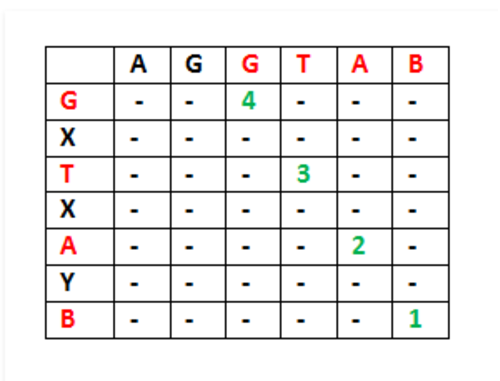
\includegraphics[width=0.5\textwidth]{Images/figGFGDPSet4LCS}
\label{figGFGDPSet4LCS}
\end{figure}
\item Consider the input strings ``ABCDGH'' and ``AEDFHR''. Last characters
  do not match for the strings. So length of LCS can be written as:\\
$L(\text{``ABCDGH''},\text{``AEDFHR''})=$\\
$MAX(L(\text{``ABCDG''},\text{``AEDFH\textbf{R}''}),L(\text{``ABCDG\textbf{H}''},\text{``AEDFH''}))$
\end{enumerate}

So the LCS problem has optimal substructure property as the main problem can
be solved using solutions to subproblems.

\rrheader{(2) Overlapping Subproblems:}

Following is simple recursive implementation of the LCS problem. The
implementation simply follows the recursive structure mentioned above.
\begin{lstlisting}[style=raycppnewsnippet]
/* A Naive recursive implementation of LCS problem */
#include<bits/stdc++.h>
 
int max(int a, int b);
 
/* Returns length of LCS for X[0..m-1], Y[0..n-1] */
int lcs( char *X, char *Y, int m, int n )
{
   if (m == 0 || n == 0)
     return 0;
   if (X[m-1] == Y[n-1])
     return 1 + lcs(X, Y, m-1, n-1);
   else
     return max(lcs(X, Y, m, n-1), lcs(X, Y, m-1, n));
}
 
/* Utility function to get max of 2 integers */
int max(int a, int b)
{
    return (a > b)? a : b;
}
 
/* Driver program to test above function */
int main()
{
  char X[] = "AGGTAB";
  char Y[] = "GXTXAYB";
 
  int m = strlen(X);
  int n = strlen(Y);
 
  printf("Length of LCS is %dn", lcs( X, Y, m, n ) );
 
  return 0;
}
\end{lstlisting}
Output:
\begin{lstlisting}[style=rayio]
Length of LCS is 4
\end{lstlisting}
Time complexity of the above naive recursive approach is $\comBigOh{(2^n)}$
in worst case and worst case happens when all characters of $X$ and $Y$
mismatch i.e., length of LCS is $0$.

Considering the above implementation, following is a partial recursion tree
for input strings ``AXYT'' and ``AYZX''
\begin{lstlisting}[style=pseudostyle]
                         lcs("AXYT", "AYZX")
                       /                 
         lcs("AXY", "AYZX")            lcs("AXYT", "AYZ")
         /                              /               
lcs("AX", "AYZX") lcs("AXY", "AYZ")   lcs("AXY", "AYZ") lcs("AXYT", "AY")
\end{lstlisting}
In the above partial recursion tree, $lcs(\text{``AXY''},\text{``AYZ''})$ is
being solved twice. If we draw the complete recursion tree, then we can see
that there are many subproblems which are solved again and again. So this
problem has Overlapping Substructure property and recomputation of same
subproblems can be avoided by either using Memoization or Tabulation.
Following is a tabulated implementation for the LCS problem.
\begin{lstlisting}[style=raycppnewsnippet]
/* Dynamic Programming C/C++ implementation of LCS problem */
#include<bits/stdc++.h>
  
int max(int a, int b);
  
/* Returns length of LCS for X[0..m-1], Y[0..n-1] */
int lcs( char *X, char *Y, int m, int n )
{
   int L[m+1][n+1];
   int i, j;
  
   /* Following steps build L[m+1][n+1] in bottom up fashion. Note 
      that L[i][j] contains length of LCS of X[0..i-1] and Y[0..j-1] */
   for (i=0; i<=m; i++)
   {
     for (j=0; j<=n; j++)
     {
       if (i == 0 || j == 0)
         L[i][j] = 0;
  
       else if (X[i-1] == Y[j-1])
         L[i][j] = L[i-1][j-1] + 1;
  
       else
         L[i][j] = max(L[i-1][j], L[i][j-1]);
     }
   }
    
   /* L[m][n] contains length of LCS for X[0..n-1] and Y[0..m-1] */
   return L[m][n];
}
/* Utility function to get max of 2 integers */
int max(int a, int b)
{
    return (a > b)? a : b;
}
  
/* Driver program to test above function */
int main()
{
  char X[] = "AGGTAB";
  char Y[] = "GXTXAYB";
  
  int m = strlen(X);
  int n = strlen(Y);
  
  printf("Length of LCS is %dn", lcs( X, Y, m, n ) );
 
  return 0;
}
\end{lstlisting}
Time Complexity of the above implementation is $\comBigOh{(mn)}$ which is
much better than the worst case time complexity of Naive Recursive
implementation.

The above algorithm/code returns only length of LCS. Please see the
following post for printing the LCS. Printing Longest Common Subsequence
(see \pagecref{secGFGDPLCSPrint})

You can also check the space optimized version of LCS at Space Optimized
Solution of LCS (see \pagecref{secGFGDPLCSSpaceOptimized})


%%%%%%%%%%%%%%%%%%%%%%%%%%%%%%%%%%%%%%%%%%%%%%%%%%%%%%%%%%%%%%%%%%%%%%%%%%%%
%%%%%%%%%%%%%%%%%%%%%%%%%%%%%%%%%%%%%%%%%%%%%%%%%%%%%%%%%%%%%%%%%%%%%%%%%%%%
%%%%%%%%%%%%%%%%%%%%%%%%%%%%%%%%%%%%%%%%%%%%%%%%%%%%%%%%%%%%%%%%%%%%%%%%%%%%

\subsection{Printing Longest Common Subsequence
  \label{secGFGDPLCSPrint}}

\url{http://www.geeksforgeeks.org/printing-longest-common-subsequence/}

\textbf{Difficulty: 3.2}

Given two sequences, print the longest subsequence present in both of them.

\rrheader{Examples:}
\begin{itemize}%[noitemsep,topsep=0pt]
\item LCS for input Sequences ``ABCDGH'' and ``AEDFHR'' is ``ADH'' of length
  3.
\item LCS for input Sequences ``AGGTAB'' and ``GXTXAYB'' is ``GTAB'' of
  length 4.
\end{itemize}

We have discussed Longest Common Subsequence (LCS) problem in a previous
post (see \pagecref{secGFGDPSet4LCS}). The function discussed there was
mainly to find the length of LCS. To find length of LCS, a 2D table $L[][]$
was constructed. In this post, the function to construct and print LCS is
discussed.

Following is detailed algorithm to print the LCS. It uses the same 2D table
$L[][]$.
\begin{enumerate}[label=\textbf{\arabic*.}]
\item Construct $L[m+1][n+1]$ using the steps discussed in previous post.
\item The value $L[m][n]$ contains length of LCS. Create a character array
  $lcs[]$ of length equal to the length of lcs plus 1 (one extra to store
  $\backslash0$ \rrblue{(\textsc{nil})}).
\item Traverse the 2D array starting from $L[m][n]$. Do following for every
  cell $L[i][j]$
  \begin{enumerate}[label=\textbf{\alph*.}]
  \item If characters (in X and Y) corresponding to $L[i][j]$ are same (Or
    $X[i-1] == Y[j-1]$), then include this character as part of LCS.
  \item Else compare values of $L[i-1][j]$ and $L[i][j-1]$ and go in
    direction of greater value.
  \end{enumerate}
\end{enumerate}

The following table (taken from
Wiki\footnote{\url{https://en.wikipedia.org/wiki/Longest\_common\_subsequence\_problem}})
shows steps (highlighted) followed by the above algorithm.

\begin{figure}
\centering
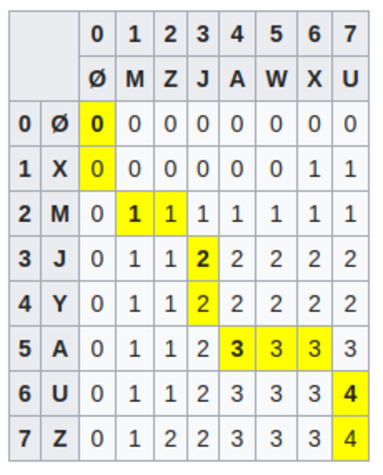
\includegraphics[width=0.4\textwidth]{Images/figGFGDPSet4LCSPrint}
\label{figGFGDPSet4LCSPrint}
\end{figure}

\textbf{\rrgreen{Recommended: Please try your approach first, before moving
    on to the solution.}}

\RayNotesBegin

This is in the same file as the lcs code:\\
\path{src/DynamicProgramming/rrrGFGLCS.cpp}
\begin{lstlisting}[style=raycppnewsnippet]
template<typename S, typename T>
auto get_lcs(S& str1, S& str2, T c)
{
  // store the lcs characters, note: since we are using arrays, we do not
  // need the terminating character.
  auto m = str1.size();
  auto n = str2.size();

  vector<std::remove_cv_t<std::remove_reference_t<decltype(str1[0])> > > 
    lcs_chars(c[m][n]);
  auto i = m;
  auto j = n;
  auto lcs_index = c[m][n];

  while(i>0 && j>0)
  {
    if(str1[i-1] == str2[j-1])
    {
      lcs_chars[lcs_index-1] = str1[i-1];
      --i; --j; --lcs_index;
    }
    // move up? Note that we do NOt minus one from c[][] indices. Since this
    // array contains 0 at the upper left.
    else if(c[i-1][j]>c[i][j-1])
      --i;
    // move to the left
    else 
      --j;
  }

  return lcs_chars;
}
\end{lstlisting}

\RayNotesEnd

Following is C++ implementation of above approach.
\begin{lstlisting}[style=raycppnewsnippet]
/* Dynamic Programming implementation of LCS problem */
#include<iostream>
#include<cstring>
#include<cstdlib>
using namespace std;
 
/* Returns length of LCS for X[0..m-1], Y[0..n-1] */
void lcs( char *X, char *Y, int m, int n )
{
   int L[m+1][n+1];
 
   /* Following steps build L[m+1][n+1] in bottom up fashion. Note
      that L[i][j] contains length of LCS of X[0..i-1] and Y[0..j-1] */
   for (int i=0; i<=m; i++)
   {
     for (int j=0; j<=n; j++)
     {
       if (i == 0 || j == 0)
         L[i][j] = 0;
       else if (X[i-1] == Y[j-1])
         L[i][j] = L[i-1][j-1] + 1;
       else
         L[i][j] = max(L[i-1][j], L[i][j-1]);
     }
   }
 
   // Following code is used to print LCS
   int index = L[m][n];
 
   // Create a character array to store the lcs string
   char lcs[index+1];
   lcs[index] = '\0'; // Set the terminating character
   
   // Start from the right-most-bottom-most corner and
   // one by one store characters in lcs[]
   int i = m, j = n;
   while (i > 0 && j > 0)
   {
      // If current character in X[] and Y are same, then
      // current character is part of LCS
      if (X[i-1] == Y[j-1])
      {
          lcs[index-1] = X[i-1]; // Put current character in result
          i--; j--; index--;     // reduce values of i, j and index
      }
 
      // If not same, then find the larger of two and
      // go in the direction of larger value
      else if (L[i-1][j] > L[i][j-1])
         i--;
      else
         j--;
   }
 
   // Print the lcs
   cout << "LCS of " << X << " and " << Y << " is " << lcs;
}
/* Driver program to test above function */
int main()
{
  char X[] = "AGGTAB";
  char Y[] = "GXTXAYB";
  int m = strlen(X);
  int n = strlen(Y);
  lcs(X, Y, m, n);
  return 0;
}
\end{lstlisting}
Output:
\begin{lstlisting}[style=rayio]
LCS of AGGTAB and GXTXAYB is GTAB
\end{lstlisting}

%%%%%%%%%%%%%%%%%%%%%%%%%%%%%%%%%%%%%%%%%%%%%%%%%%%%%%%%%%%%%%%%%%%%%%%%%%%%
%%%%%%%%%%%%%%%%%%%%%%%%%%%%%%%%%%%%%%%%%%%%%%%%%%%%%%%%%%%%%%%%%%%%%%%%%%%%
%%%%%%%%%%%%%%%%%%%%%%%%%%%%%%%%%%%%%%%%%%%%%%%%%%%%%%%%%%%%%%%%%%%%%%%%%%%%

\subsection{A Space Optimized Solution of LCS
  \label{secGFGDPLCSSpaceOptimized}}

\url{http://www.geeksforgeeks.org/space-optimized-solution-lcs}

\textbf{Difficulty: 2.5}

TODO

%%%%%%%%%%%%%%%%%%%%%%%%%%%%%%%%%%%%%%%%%%%%%%%%%%%%%%%%%%%%%%%%%%%%%%%%%%%%
%%%%%%%%%%%%%%%%%%%%%%%%%%%%%%%%%%%%%%%%%%%%%%%%%%%%%%%%%%%%%%%%%%%%%%%%%%%%
%%%%%%%%%%%%%%%%%%%%%%%%%%%%%%%%%%%%%%%%%%%%%%%%%%%%%%%%%%%%%%%%%%%%%%%%%%%%

\section{Dynamic Programming | Set 5 (Edit Distance)
  \label{secGFGDPSet5EditDistance}}

\url{http://www.geeksforgeeks.org/dynamic-programming-set-5-edit-distance}

\textbf{Difficulty: 3.3}

Given two strings str1 and str2 and below operations that can performed on
str1. Find minimum number of edits (operations) required to convert ``str1''
into ``str2''.
\begin{enumerate}[label=\textbf{\alph*.}]
\item Insert
\item Remove
\item Replace
\end{enumerate}
All of the above operations are of equal cost.

\begin{mdframed}[style=mdfNOTE,
frametitle={Examples:}]
\begin{lstlisting}[style=raygeneric]
Input:   str1 = "geek", str2 = "gesek"
Output:  1
We can convert str1 into str2 by inserting a 's'.

Input:   str1 = "cat", str2 = "cut"
Output:  1
We can convert str1 into str2 by replacing 'a' with 'u'.

Input:   str1 = "sunday", str2 = "saturday"
Output:  3
Last three and first characters are same.  We basically
need to convert "un" to "atur".  This can be done using
below three operations. 
Replace 'n' with 'r', insert t, insert a
\end{lstlisting}
\end{mdframed}

\textbf{\rrgreen{Recommended: Please try your approach first, before moving
    on to the solution.}}

\RayNotesBegin

First let's recall the steps to solve a DP problem:
\begin{enumerate}[label=\textbf{\arabic*.}]
\item Identify if it is a DP problem: I.e. do we have an optimal
  substructure and overlapping subproblems?
\item Decide on a state expression with least parameters: What parameters
  describe the problem/solution?
\item Formulate state relationship: Say if we have the solution for $i$, we
  have to put it in terms of the solutions previous to $i$.
\item Do tabulation (or add memoization): Choose one!
\end{enumerate}

Again, we'll do states \textbf{(1)}--\textbf{(2)} together. We'll try to
edit str1 into str2, for convenience, let's call them $X[0..m]$ and
$Y[0..n]$. We'll start at the end of the strings. First thing to do is to
compare the ends to see if they are the same. If they are, nothing needs to
be done. If they are not, then we perform all three \rrhl{actions} on $X$ to
try convert it into $Y$. This is kind of similar to the minimum number of
coins problem where we start at the last value and add all the possible coin
types (this is the \rrhl{action}), and choose the min of the resulting
sub-problem plus 1 for the coin type we've added. So in detail:
\begin{enumerate}[label=\textbf{\arabic*.}]
\item If $X[i]==Y[j]$, no action taken, recur for $X[i-1]$ and $Y[j-1]$.
\item Else $X[i]\neq Y[j]$. Let's say we have: $X=\braket*{?,?,\ldots,?,a}$
  and $Y=\braket*{?,?,\ldots,?,b}$, then:
  \begin{enumerate}[label=\textbf{\alph*.}]
  \item Insert into $X$: $X=\braket*{?,?,\ldots,?,a,b}$,
    $Y=\braket*{?,?,\ldots,?,b}$. We have used $1$ operation. The last two
    chars are now the same. This increases the length of $X$ by one, so we 
    can recur for $X[0..i]$ and $Y[0..j-1]$ to repeat the algorithm for 
    $X=\braket*{?,?,\ldots,?,a}$ and $Y=\braket*{?,?,\ldots,?}$.
  \item Replace into $X$: $X=\braket*{?,?,\ldots,?,b}$, 
    $Y=\braket*{?,?,\ldots,?,b}$. The last two chars are now the same.
    Neither of the strings have increased in length, so we recur for
    $X[0..i-1]$ and $Y[0..j-1]$ to repeat the algo for 
    $X=\braket*{?,?,\ldots,?}$ and $Y=\braket*{?,?,\ldots,?}$.
  \item Remove from $X$: In this case we end up having $X=\braket*{?,?,\ldots,?}$
  and $Y=\braket*{?,?,\ldots,?,b}$. Thus we must repeat the algo for
  $X[0..i-1]$ and $Y[0..j]$ to test again.
  \end{enumerate}
\end{enumerate}

Base cases: If $X.size()==0$, then we simply insert what's left from $Y$
into $X$, the number of edits will increase by that amount. If
$Y.size()==0$, then we simply remove what's left from $X$, the number of
edits will increase by the same amount removed.

\qasepline{}

Before we start implementing, let's see how this relates to LCS (seeing if I
can find some sort of a pattern with these DP problems).

In both Edit Distance and LCS, we compare the last character. If they are
the same, then LCS: increase the LCS length and recur; Edit Distance: do not
add an edit and recur. If the last characters are not the same, then in Edit
Distance (and similarly to the minimum coin type problem) we perform all the
actions and recur to get the minimum. For LCS however, the action requires
some intuition, it's simply just running the LCS algo again, but on
$(X[0..i-1],Y[0..j])$ or $(X[0..i],Y[0..j])$. There are no actions to take
but we can run the algo on a smaller state by the intuition of the lcs must
be in $(X_{i-1},Y_{j})$ or $(X_{i},Y_{j-1})$, so we take the maximum of
that.

\qasepline{}

Now onto coding! We first do a simple recursion, then decide on tabulation
or memoization. Code is found in\\
\path{src/DynamicProgramming/rrrGFGDPSet5EditDist.cpp}
\begin{lstlisting}[style=raycppnewsnippet]
template<typename T>
auto editDist(const T& s1, const T& s2, 
              decltype(s1.size()) s1_sz, decltype(s2.size()) s2_sz)
{
  // Insert all elements from s2 into s1, therefore number of edits
  // is the same as the number of chars left in s2.
  if(s1_sz == 0)
  {
    return s2_sz;
  }
  // If s2 is empty, then we remove all the chars left in s1. The number of
  // edits is the same as the number of chars in s1.
  if(s2_sz == 0)
  {
    return s1_sz;
  }
  
  // If the last character of the two strings are the same, we do not add
  // an edit. We just recur.
  if(s1[s1_sz-1]==s2[s2_sz-1])
    return editDist(s1,s2,s1_sz-1,s2_sz-1);

  // Last chars are different, so we use an edit (insert/remove/replace)
  // and recur.
  return 1 + min({editDist(s1,s2,s1_sz,s2_sz-1),    // insert
                  editDist(s1,s2,s1_sz-1,s2_sz),    // remove
                  editDist(s1,s2,s1_sz-1,s2_sz-1)});// replace
}
\end{lstlisting}
With DP and tabulation:
\begin{lstlisting}[style=raycppnewsnippet]
// Now we do DP with tabulation (bottom up, starting with top left,
// i.e. i=0, j=0, and work to i=)
auto editDistTabulate(const string& s1, const string& s2)
{
  using strsz_t = decltype(s1.size());

  auto m = s1.size();
  auto n = s2.size();

  // minDist[i][j] contains the min edits for strs of length i and j,
  // where 0<=i<=m and 0<=j<=n
  // This is why we plus 1 to the sizes.
  vector<vector<strsz_t>>
    minDist(m+1,vector<strsz_t>(n+1,0));

  // Fill in minDist in bottom up manner, first loop through the rows.
  for(strsz_t i = 0; i != (m+1); ++i)
  {
    // Loop through each column.
    for(strsz_t j = 0; j != (n+1); ++j)
    {
      // If first string is empty, only option is to insert all chars of
      // second string
      if(i == 0) 
        minDist[i][j] = j; // Min. edits = j

      // If second string is empty, only option is to remove all chars of
      // the first string.
      else if(j==0) 
        minDist[i][j] = i; // Min. edits = i

      // If the last chars are the same, ignore last char (no edits 
      // required), and recur for remaining string.
      else if(s1[i]==s2[j])
        minDist[i][j] = minDist[i-1][j-1];

      // If last char are different, consider all possibilities and find
      // the minimum.
      else
        minDist[i][j] = 1+std::min({minDist[i][j-1],    // insert
                                    minDist[i-1][j],    // remove
                                    minDist[i-1][j-1]});// replace
    }
  }
  return minDist[m][n];
}
\end{lstlisting}

\RayNotesEnd

\textbf{\rrgreen{Back to geeksforgeeks solution.}}

\rrheader{What are the subproblems in this case?}

The idea is process all characters one by one staring from either from left
or right sides of both strings.

Let we traverse from right corner, there are two possibilities for every
pair of character being traversed.
\begin{itemize}%[noitemsep,topsep=0pt]
\item \textbf{m}: Length of str1 (first string)
\item \textbf{n}: Length of str2 (second string)
\end{itemize}
\begin{enumerate}[label=\textbf{\arabic*.}]
\item If last characters of two strings are same, nothing much to do. Ignore
  last characters and get count for remaining strings. So we recur for
  lengths $m-1$ and $n-1$.
\item Else (If last characters are not same), we consider all operations on
  ``str1'', consider all three operations on last character of first string,
  recursively compute minimum cost for all three operations and take minimum
  of three values.
  \begin{enumerate}[label=\textbf{\alph*.}]
  \item Insert: Recur for m and n-1
  \item Remove: Recur for m-1 and n
  \item Replace: Recur for m-1 and n-1
  \end{enumerate}
\end{enumerate}
Below is C++ implementation of above Naive recursive solution.
\begin{lstlisting}[style=raycppnewsnippet]
// A Naive recursive C++ program to find minimum number
// operations to convert str1 to str2
#include<bits/stdc++.h>
using namespace std;
 
// Utility function to find minimum of three numbers
int min(int x, int y, int z)
{
   return min(min(x, y), z);
}
 
int editDist(string str1 , string str2 , int m ,int n)
{
    // If first string is empty, the only option is to
    // insert all characters of second string into first
    if (m == 0) return n;
 
    // If second string is empty, the only option is to
    // remove all characters of first string
    if (n == 0) return m;
 
    // If last characters of two strings are same, nothing
    // much to do. Ignore last characters and get count for
    // remaining strings.
    if (str1[m-1] == str2[n-1])
        return editDist(str1, str2, m-1, n-1);
 
    // If last characters are not same, consider all three
    // operations on last character of first string, recursively
    // compute minimum cost for all three operations and take
    // minimum of three values.
    return 1 + min ( editDist(str1,  str2, m, n-1),    // Insert
                     editDist(str1,  str2, m-1, n),   // Remove
                     editDist(str1,  str2, m-1, n-1) // Replace
                   );
}

// Driver program
int main()
{
    // your code goes here
    string str1 = "sunday";
    string str2 = "saturday";
 
    cout << editDist( str1 , str2 , str1.length(), str2.length());
 
    return 0;
}
\end{lstlisting}
Output:
\begin{lstlisting}[style=rayio]
3
\end{lstlisting}
The time complexity of above solution is exponential. In worst case, we may
end up doing $\comBigOh{3^m}$ operations. The worst case happens when none of
characters of two strings match. Below is a recursive call diagram for worst
case.

\begin{figure}
\centering
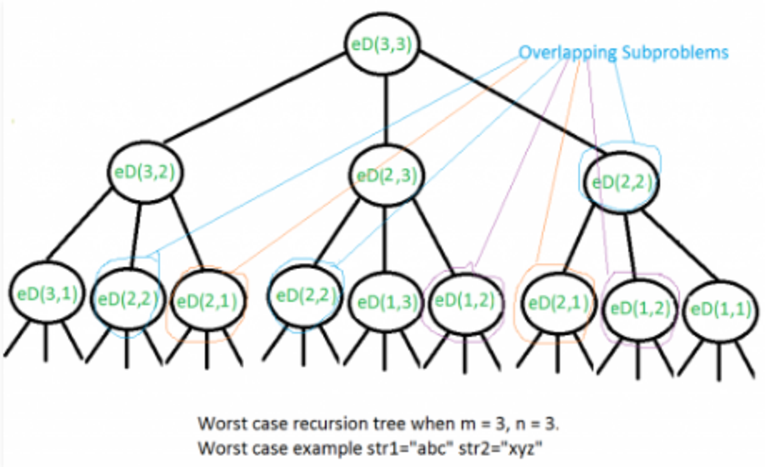
\includegraphics[width=0.7\textwidth]{Images/figGFGDPSet5EditDist}
\label{figGFGDPSet5EditDist}
\end{figure}

We can see that many subproblems are solved again and again, for example
\ctt{eD(2,2)} is called three times. Since same suproblems are called again,
this problem has Overlapping Subprolems property. So Edit Distance problem
has both properties (see this and this) of a dynamic programming problem.
Like other typical Dynamic Programming(DP) problems, recomputations of same
subproblems can be avoided by constructing a temporary array that stores
results of subpriblems.
\begin{lstlisting}[style=raycppnewsnippet]
// A Dynamic Programming based C++ program to find minimum
// number operations to convert str1 to str2
#include<bits/stdc++.h>
using namespace std;
 
// Utility function to find minimum of three numbers
int min(int x, int y, int z)
{
    return min(min(x, y), z);
}

int editDistDP(string str1, string str2, int m, int n)
{
  // Create a table to store results of subproblems
  int dp[m+1][n+1];
 
  // Fill d[][] in bottom up manner
  for (int i=0; i<=m; i++)
  {
    for (int j=0; j<=n; j++)
    {
      // If first string is empty, only option is to
      // isnert all characters of second string
      if (i==0)
          dp[i][j] = j;  // Min. operations = j
 
      // If second string is empty, only option is to
      // remove all characters of second string
      else if (j==0)
          dp[i][j] = i; // Min. operations = i
 
      // If last characters are same, ignore last char
      // and recur for remaining string
      else if (str1[i-1] == str2[j-1])
          dp[i][j] = dp[i-1][j-1];
 
      // If last character are different, consider all
      // possibilities and find minimum
      else
        dp[i][j] = 1 + min(dp[i][j-1],  // Insert
                           dp[i-1][j],  // Remove
                           dp[i-1][j-1]); // Replace
    }
  }
  return dp[m][n];
}
// Driver program
int main()
{
    // your code goes here
    string str1 = "sunday";
    string str2 = "saturday";
 
    cout << editDistDP(str1, str2, str1.length(), str2.length());
 
    return 0;
}
\end{lstlisting}
Output:
\begin{lstlisting}[style=rayio]
3
\end{lstlisting}

\noindent{}\textbf{Time Complexity: O(m x n)}\\
\noindent{}\textbf{Auxiliary Space: O(m x n)}

\textbf{Applications:} There are many practical applications of edit
distance algorithm, refer
Lucene\footnote{\url{http://en.wikipedia.org/wiki/Lucene}} API for sample.
Another example, display all the words in a dictionary that are near
proximity to a given wordincorrectly spelled word.

%%%%%%%%%%%%%%%%%%%%%%%%%%%%%%%%%%%%%%%%%%%%%%%%%%%%%%%%%%%%%%%%%%%%%%%%%%%%
%%%%%%%%%%%%%%%%%%%%%%%%%%%%%%%%%%%%%%%%%%%%%%%%%%%%%%%%%%%%%%%%%%%%%%%%%%%%
%%%%%%%%%%%%%%%%%%%%%%%%%%%%%%%%%%%%%%%%%%%%%%%%%%%%%%%%%%%%%%%%%%%%%%%%%%%%

\section{Dynamic Programming | Set 6 (Min Cost Path)
  \label{secGFGDPSet6MinCostPath}}

\url{http://www.geeksforgeeks.org/dynamic-programming-set-6-min-cost-path/}

\textbf{Difficulty: 2.4}

Given a cost matrix \ctt{cost[][]} and a position $(m, n)$ in
\ctt{cost[][]}, write a function that returns cost of minimum cost path to
reach $(m,n)$ from $(0,0)$. Each cell of the matrix represents a cost to
traverse through that cell. Total cost of a path to reach $(m,n)$ is sum of
all the costs on that path (including both source and destination).
\textbf{You can only traverse \emph{down}, \emph{right} and
  \emph{diagonally} lower cells} from a given cell, i.e., from a given cell
$(i,j)$, cells $(i+1,j)$, $(i,j+1)$ and $(i+1,j+1)$ can be traversed. You
may assume that all costs are positive integers.

For example, in the following figure, what is the minimum cost path to 
$(2,2)$?

\begin{figure}
\centering
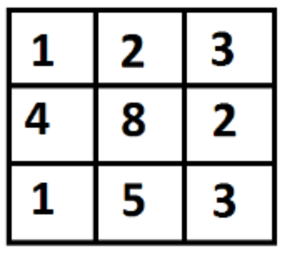
\includegraphics[width=0.2\textwidth]{Images/figGFGDPSet6MinCostPath1}
\label{figGFGDPSet6MinCostPath1}
\end{figure}

The path with minimum cost is highlighted in the following figure. The path
is $(0,0)\to(0,1)\to(1,2)\to(2,2)$. The cost of the path is $8=(1+2+2+3)$.

\begin{figure}
\centering
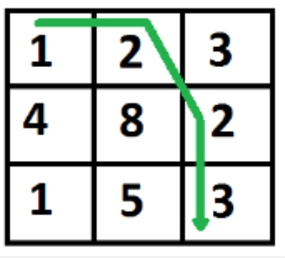
\includegraphics[width=0.2\textwidth]{Images/figGFGDPSet6MinCostPath2}
\label{figGFGDPSet6MinCostPath2}
\end{figure}

\textbf{\rrgreen{Recommended: Please try your approach first, before moving
    on to the solution.}}

\RayNotesBegin

Okay, first we develop the \textbf{optimal substructure}, the
\textbf{states}, and the \textbf{recurrence relation}. How do we go about
this? Remember that we have to try and build the current optimal solution
(in this case to take the min) with a choice of previous optimal solutions.

Say we are at cell $(i,j)$. We could have only reached $(i,j)$ from top
$(i-1,j)$, left $(i,j-1)$ and diagonal $(i-1,j-1)$. \rrhl{These are my three
  actions which I must choose from}. So we have the
recurrence relation:
\begin{equation*}
\text{mC}(i,j)
=\text{c}[i][j]+\min(\text{mC}(i-1,j),\text{mC}(i,j-1),\text{mC}(i-1,j-1))
\end{equation*}
where mC is the minCost function, and c is is the table of costs.
Note that this works because $(i,j)$ depends only on previous solutions.
Otherwise, this problem might get very hard. 

What about base cases and edge cases? The base case (where the recursion
ends) happens at $(i=0,j=0) =\text{c}[0][0]$. For edge cases, we have the
first/top row and the first/left column.
\begin{itemize}%[noitemsep,topsep=0pt]
\item Top row $(i=0,j\neq0)$: cell $(i,j)$ can only be reached from the left
  cell $(i,j-1)$, which gives:
  \begin{equation*}
  \text{mC}(i,j) = \text{c}[i][j]+\text{mC}(i,j-1) \text{ for $i=0,j\neq0$}
  \end{equation*}
\item First column $(i\neq0,j=0)$: cell $(i,j)$ can only be reached from the
  top cell $(i-1,j)$, which gives:
  \begin{equation*}
  \text{mC}(i,j) = \text{c}[i][j]+\text{mC}(i-1,j) \text{ for $i\neq0,j=0$}
  \end{equation*}
\end{itemize}
Now let's code this up. Code found here:\\
\path{src/DynamicProgramming/rrrGFGDPSet6MinCostPath.cpp}
\begin{lstlisting}[style=raycppnewsnippet]
template<typename T>
auto minCost(vector<vector<T>>&cost, size_t m, size_t n)
{
  if(m==0 && n==0)
    return cost[m][n];
  if(m==0 && n != 0)
    return cost[m][n] + minCost(cost,m,n-1);
  if(m!=0 && n==0)
    return cost[m][n] + minCost(cost,m-1,n);

  return cost[m][n] + std::min({minCost(cost,m,n-1),    // left
                                minCost(cost,m-1,n),    // top
                                minCost(cost,m-1,n-1)});// diag
}
\end{lstlisting}
Now for the DP version using bottom up with tabulation
\begin{lstlisting}[style=raycppnewsnippet]
template<typename T>
auto minCostDP(vector<vector<T>>&cost, size_t m, size_t n)
{
  // table of min costs
  // since m and n are used to index the cost table directly, they are one
  // smaller the cost table's sizes. So we +1 when we declare it and give 
  // the size.
  vector<vector<T>> mc(m+1,vector<T>(n+1,T{}));

  using vecsz_t = decltype(cost.size());

  // Take care of base case and edge cases:
  mc[0][0] = cost[0][0];

  // first column
  // Note that we need less than or equal to, since these m and n are used
  // to index the vectors directly. I.e. they range from 0 to cost.size()-1
  for(vecsz_t i = 1; i <= m; ++i)
    mc[i][0] = cost[i][0] + mc[i-1][0];
  
  // first row
  for(vecsz_t j = 1; j <= n; ++j)
    mc[0][j] = cost[0][j] + mc[0][j-1];

  // Now we work in row major order, from first row, then 2nd row, etc...
  for(vecsz_t i = 1; i <= m; ++i)
  {
    for(vecsz_t j = 1; j <= n; ++j)
    {
      mc[i][j] = cost[i][j] + std::min({mc[i-1][j],    // top
                                        mc[i][j-1],    // left
                                        mc[i-1][j-1]});// diag
    }
  }
  // Recall that m and n are not the sizes, we use it to directly index, so 
  // we do not take one off, i.e. not mc[m-1][n-1]
  return mc[m][n];
}
\end{lstlisting}

\RayNotesEnd

\textbf{\rrgreen{Back to geeksforgeeks solution.}}

\rrheader{(1) Optimal Substructure}
The path to reach $(m,n)$ must be through one of the 3 cells: $(m-1,n-1)$ or
$(m-1,n)$ or $(m,n-1)$. So minimum cost to reach $(m,n)$ can be written as
``minimum of the 3 cells plus cost$[m][n]$'':
\begin{equation*}
\text{minCost}(m, n)
=\min(\text{minCost}(m-1,n-1),
      \text{minCost}(m-1, n),
      \text{minCost}(m,n-1))
      +cost[m][n]
\end{equation*}

\rrheader{(2) Overlapping Subproblems}
Following is simple recursive implementation of the MCP (Minimum Cost Path)
problem. The implementation simply follows the recursive structure mentioned
above.
\begin{lstlisting}[style=raycppnewsnippet]
/* A Naive recursive implementation of MCP(Minimum Cost Path) problem */
#include<stdio.h>
#include<limits.h>
#define R 3
#define C 3
 
int min(int x, int y, int z);
 
/* Returns cost of minimum cost path from (0,0) to (m, n) in mat[R][C]*/
int minCost(int cost[R][C], int m, int n)
{
   if (n < 0 || m < 0)
      return INT_MAX;
   else if (m == 0 && n == 0)
      return cost[m][n];
   else
      return cost[m][n] + min( minCost(cost, m-1, n-1),
                               minCost(cost, m-1, n), 
                               minCost(cost, m, n-1) );
}
 
/* A utility function that returns minimum of 3 integers */
int min(int x, int y, int z)
{
   if (x < y)
      return (x < z)? x : z;
   else
      return (y < z)? y : z;
}

/* Driver program to test above functions */
int main()
{
   int cost[R][C] = { {1, 2, 3},
                      {4, 8, 2},
                      {1, 5, 3} };
   printf(" %d ", minCost(cost, 2, 2));
   return 0;
}
\end{lstlisting}
It should be noted that the above function computes the same subproblems
again and again. See the following recursion tree, there are many nodes
which apear more than once. Time complexity of this naive recursive solution
is exponential and it is terribly slow.
\begin{lstlisting}[style=raygeneric]
mC refers to minCost()
                                mC(2, 2)
                      /            |           \
                     /             |            \             
             mC(1, 1)           mC(1, 2)             mC(2, 1)
          /     |     \       /     |     \           /     |     \ 
         /      |      \     /      |      \         /      |       \
   mC(0,0) mC(0,1) mC(1,0) mC(0,1) mC(0,2) mC(1,1) mC(1,0) mC(1,1) mC(2,0) 
\end{lstlisting}
So the MCP problem has both properties (see
\pagecref{secGFGDPSet1OverlapSubprob} and
\pagecref{secGFGDPSet2OptimalSubstruct}) of a dynamic programming problem.
Like other typical Dynamic Programming(DP) problems, recomputations of same
subproblems can be avoided by constructing a temporary array \ctt{tc[][]} in
bottom up manner.
\begin{lstlisting}[style=raycppnewsnippet]
/* Dynamic Programming implementation of MCP problem */
#include<stdio.h>
#include<limits.h>
#define R 3
#define C 3
 
int min(int x, int y, int z);
 
int minCost(int cost[R][C], int m, int n)
{
     int i, j;
 
     // Instead of following line, we can use int tc[m+1][n+1] or 
     // dynamically allocate memoery to save space. The following line is
     // used to keep te program simple and make it working on all compilers.
     int tc[R][C];  
 
     tc[0][0] = cost[0][0];
 
     /* Initialize first column of total cost(tc) array */
     for (i = 1; i <= m; i++)
        tc[i][0] = tc[i-1][0] + cost[i][0];
 
     /* Initialize first row of tc array */
     for (j = 1; j <= n; j++)
        tc[0][j] = tc[0][j-1] + cost[0][j];
 
     /* Construct rest of the tc array */
     for (i = 1; i <= m; i++)
        for (j = 1; j <= n; j++)
            tc[i][j] = min(tc[i-1][j-1], 
                           tc[i-1][j], 
                           tc[i][j-1]) + cost[i][j];
 
     return tc[m][n];
}
/* A utility function that returns minimum of 3 integers */
int min(int x, int y, int z)
{
   if (x < y)
      return (x < z)? x : z;
   else
      return (y < z)? y : z;
}
 
/* Driver program to test above functions */
int main()
{
   int cost[R][C] = { {1, 2, 3},
                      {4, 8, 2},
                      {1, 5, 3} };
   printf(" %d ", minCost(cost, 2, 2));
   return 0;
}
\end{lstlisting}
Output
\begin{lstlisting}[style=rayio]
8
\end{lstlisting}
\rrhl{Time Complexity of the DP implementation is} $\comBigOh{mn}$ which is
much better than Naive Recursive implementation.

Asked in:
Amazon\footnote{\url{https://practice.geeksforgeeks.org/company/Amazon/}}

%%%%%%%%%%%%%%%%%%%%%%%%%%%%%%%%%%%%%%%%%%%%%%%%%%%%%%%%%%%%%%%%%%%%%%%%%%%%
%%%%%%%%%%%%%%%%%%%%%%%%%%%%%%%%%%%%%%%%%%%%%%%%%%%%%%%%%%%%%%%%%%%%%%%%%%%%
%%%%%%%%%%%%%%%%%%%%%%%%%%%%%%%%%%%%%%%%%%%%%%%%%%%%%%%%%%%%%%%%%%%%%%%%%%%%

\section{Dynamic Programming | Set 7 (Coin Change)
  \label{secGFGDPSet7CoinChange}}

\url{http://www.geeksforgeeks.org/dynamic-programming-set-7-coin-change}

\textbf{Difficulty: 3.7}

Given a value $N$, if we want to make change for $N$ cents, and we have
infinite supply of each of $S=\brce*{S_1, S_2,\ldots,S_m}$ valued coins,
\rrhl{how many ways can we make the change?} The order of coins doesn't
matter.

For example, for $N=4$ and $S=\brce*{1,2,3}$, there are four solutions:
$\brce*{1,1,1,1}$, $\brce*{1,1,2}$, $\brce*{2,2}$, $\brce*{1,3}$. So output
should be $4$. For $N=10$ and $S=\brce*{2,5,3,6}$, there are five solutions:
$\brce*{2,2,2,2,2}$, $\brce*{2,2,3,3}$, $\brce*{2,2,6}$, $\brce*{2,3,5}$ and
$\brce*{5,5}$. So the output should be $5$.

\textbf{\rrgreen{Recommended: Please try your approach first, before moving
    on to the solution.}}

\RayNotesBegin

Let's look at the examples again. For $N=4$ and $S=\brce*{1,2,3}$, there are
four solutions. However, if we loop through the coins and try to use them
one by one, we get this:
\begin{lstlisting}[style=raygeneric]
1 + totalcom(n=3):
1 + 3*
1 + 2 + 1*
1 + 1 + 2*
1 + 1 + 1 + 1

2 + totalcom(n=2):
2 + 2
2 + 1 + 1*

3 + totalcom(n=1)
3 + 1*
\end{lstlisting}
So there are seven ways, the ones marked by \ctt{*} are... so this is the
incorrect substructure. Apparently, the optimal substructure comes from
integer
partition\footnote{https://en.wikipedia.org/wiki/Partition\_(number\_theory)}.

I'll just continue with the GFG solution, and also with
\url{http://www.algorithmist.com}.

\RayNotesEnd

From \url{http://www.algorithmist.com/index.php/Coin\_Change}

\rrheader{Coin Change}

\textbf{Coin Change} is the problem of finding the number of ways of making
changes for a particular amount of cents, $n$, using a given set of
denominations $d_{1}\ldots d_{m}$. It is a general case of Integer
Partition, and can be solved with dynamic programming. (The Min-Coin
Change\footnote{http://www.algorithmist.com/index.php/Min-Coin\_Change} is a
common variation of this problem.)

\rrheader{Overview}

The problem is typically asked as: If we want to make change of $N$ cents,
and we have infinite supply of each $S=\brce*{S_1,S_2,\ldots,S_m}$ valued
coins, \rrhl{how many ways can we make the change?} (For simplicity's sake,
the order does not matter.)

It is more precisely defined as:
\begin{quotation}
Given an integer $N$ and a set of integers $S=\brce*{S_1,S_2,\ldots,S_m}$,
how many ways can one express $N$ as a linear combination of
$S=\brce*{S_1,S_2,\ldots,S_m}$ with non-negative coefficients? 
\end{quotation}
Mathematically, how many solutions are there to $N=\sum_{k=1..m}x_kS_k$
where $x_k\geq0, k\in\brce*{1..m}$.  For example, for $N=4,
S=\brce*{1,2,3}$, there are four solutions: $\brce*{1,1,1,1}$,
$\brce*{1,1,2}$, $\brce*{2,2}$, $\brce*{1,3}$.

Other common variations on the problem include decision-based questions,
such as:
\begin{itemize}%[noitemsep,topsep=0pt]
\item Is there a solution for $N=\sum_{k=1..m}x_kS_k$ where $x_k\geq0,
  k\in\brce*{1..m}$ (Is there a solution for integer $N$ and a set of
  integers $S=\brce*{S_1,S_2,\ldots,S_m}$?) \rrgreen{(Solution is to check
    if the number of combination of coins is equal to zero. ezpz.)}
\item Is there a solution for $N =\sum_{k=1..m}x_kS_k$ where
  $x_k\geq0,k\in\brce*{1..m}$, $\sum_{k=1..m}x_k\leq T$ (Is there a solution
  for integer $N$) and a set of integers $S=\brce*{S_1,S_2,\ldots,S_m}$ such
  that $\sum_{k=1..m}x_k\leq T$ - using at most $T$ coins)
\end{itemize}

\rrheader{Recursive Formulation}

\textbf{We are trying to count the number of distinct sets.}

The set f solutions for this problem, $C(N,m)$, cn be partitioned into two
sets:
\begin{itemize}%[noitemsep,topsep=0pt]
\item There are those sets that do not contain any $S_m$ and
\item Those sets that contain at least one $S_m$
\end{itemize}
\begin{enumerate}[label=\textbf{\alph*.}]
\item If a solution does not contain $S_m$, then we can solve the subproblem
  of $N$ with $S=\brce*{S_1,S_2,\ldots,S_{m-1}}$, or the solution of
  $C(N,m-1)$.
\item If a solution does contain $S_m$, then we are using at least one
  $S_m$, thus we are now solving the subproblem of $N-S_m$,
  $S=\brce*{S_1,S_2,\ldots,S_m}$. This is $C(N-S_m, m)$.
\end{enumerate}
\rrblue{(This covers all of the possibilities.)} Thus, we can formulate the
following:
\begin{equation*}
C(N,m) = C(N,m-1)+C(N-S_m,m)
\end{equation*}
with the base cases:
\begin{itemize}%[noitemsep,topsep=0pt]
\item $N=0$ (number of ways to make a sum of 0) implies $C(N,m) = 1$ (one
  solution -- we have no money, exactly one way to solve the problem - by
  choosing no coin change, or, more precisely, to choose coin change of $0$)
\item $N<0$ implies $C(N,m)=0$. (negative sum of money, means we took a
  recursive path which leads to no solution, e.g. if we have $N=5$, and we
  choose to let $S_m=10$ be one of the coins) (no solution -- negative sum
  of money. This can happen along a path ending in $C(N-S_m,m)$.)
\item $N=\geq 1, m\leq 0$, (still money left but no change) implies $C(N,m)
  = 0$. (This can happen along a path ending in $C(N,m-1)$.) 
\end{itemize}

Pseudocode:
\begin{lstlisting}[style=pseudostyle]
int count(int n, int m)
{
  // m < 0 for zero indexed programming languages
  if(n<0 || m<=0)
  {
    return 0;
  }
  // needs be checked after n & m, 
  // as if n = 0 and m < 0 then it would return 1, 
  // which should not be the case.
  if(n==0)
  {
    return 1;
  }
  return count(n,m-1)+count(n-S[m],m)
}
\end{lstlisting}


\rrheader{Dynamic Programming}

Note that the recursion satisfies the weak ordering
\begin{equation*}
R(n,m)<R(x,y)\iff n\leq x,m\leq y, (n,m)\neq (x,y).
\end{equation*}
As a result, this satisfies the optimal-substructure property of dynamic
programming.

The result can be computed in $\comBigOh{nm}$ time - the above pseudocode
can easily be modified to contain memoization. It can be also rewritten as:
\begin{lstlisting}[style=pseudostyle]
func count( n, m )

  for i from 0 to n+1
    for j from 0 to m
      if i equals 0
         table[i, j] = 1          
      else if j equals 0
         if i%S[j] equals 0
               table[i, j] = 1  
         else 
               table[i, j] = 0;
      else if S[j] greater than i
         table[i, j] = table[i, j - 1]
      else 
         table[i, j] = table[i - S[j], j] + table[i, j-1]

  return table[n, m-1]
\end{lstlisting}

\rrsepline{}

\textbf{\rrgreen{Back to geeksforgeeks solution.}}

\rrheader{(1) Optimal Substructure}

To count total number solutions, we can divide all set solutions in two
sets.
\begin{enumerate}[label=\textbf{\arabic*.}]
\item Solutions that do not contain $m$th coin (or $S_m$).
\item Solutions that contain at least one $S_m$.
\end{enumerate}
Let count($S[]$, $m$, $n$) be the function to count the number of solutions,
then it can be written as sum of count($S[]$, $m-1$, $n$) and count($S[]$,
$m$, $n-S_m$).

Therefore, the problem has optimal substructure property as the problem can
be solved using solutions to subproblems.

\rrheader{(2) Overlapping Subproblems}

Following is a simple recursive implementation of the Coin Change problem.
The implementation simply follows the recursive structure mentioned above.
\begin{lstlisting}[style=raycppnewsnippet]
#include<stdio.h>
 
// Returns the count of ways we can sum  S[0...m-1] coins to get sum n
int count( int S[], int m, int n )
{
  // If n is 0 then there is 1 solution (do not include any coin)
  if (n == 0)
    return 1;
   
  // If n is less than 0 then no solution exists
  if (n < 0)
    return 0;
 
  // If there are no coins and n is greater than 0, then no solution exist
  if (m <=0 && n >= 1)
    return 0;
 
  // count is sum of solutions (i) including S[m-1] (ii) excluding S[m-1]
  return count( S, m - 1, n ) + count( S, m, n-S[m-1] );
}
 
// Driver program to test above function
int main()
{
  int i, j;
  int arr[] = {1, 2, 3};
  int m = sizeof(arr)/sizeof(arr[0]);
  printf("%d ", count(arr, m, 4));
  getchar();
  return 0;
}
\end{lstlisting}

\RayNotesBegin

This is my version, found in\\
\path{src/DynamicProgramming/rrrGFGDPSet7CoinChange.cpp}
\begin{lstlisting}[style=raycppnewsnippet]
// Recursively return the count = the number of ways to partition a sum of 
// n using coins in S[0..m-1]. Note that m represents the number of types of
// coins, so the valid inputs are [1..m], but when we index the S array, we
// do S[0..m-1].
int count(vector<int>& S, int m, int n)
{
  // If the sum n is less than 0, then no solution exists.
  if(n<0)
    return 0;

  // If n is greater than 0 and there are no coins left, then there is no
  // solution.
  if(n>=1 && m<=0)
    return 0;

  // If n is 0 then there is 1 solution (do not include any coin)
  if(n==0)
    return 1;
  
  // count is the sum of solution (i) including S[m-1] (ii) excluding S[m-1]
  return count(S,m-1,n) + count(S,m,n-S[m-1]);
}
\end{lstlisting}

\RayNotesEnd

It should be noted that the above function computes the same subproblems
again and again. See the following recursion tree for $S=\brce*{1,2,3}$ and
$n=5$. The function $C(\brce*{1}, 3)$ is called two times. If we draw the
complete tree, then we can see that there are many subproblems being called
more than once. \rrhl{Also note that each path of the recursion tree
  corresponds to one attempt at forming} $\bm{N}$ \rrhl{with the coin types,
  ending with one of the base cases. This will cover all possibilities, even
  those which makes no sense (no solution).}
\begin{lstlisting}[style=raygeneric]
C() --> count()
                              C({1,2,3}, 5)                     
                           /                
                         /                                 
             C({1,2,3}, 2)                 C({1,2}, 5)
            /                             /         
           /                             /           
C({1,2,3}, -1)  C({1,2}, 2)        C({1,2}, 3)    C({1}, 5)
               /                 /                /     
             /                  /                /       
    C({1,2},0)  C({1},2)   C({1,2},1) C({1},3)    C({1}, 4)  C({}, 5)
                   /       /        /         /         
                  /       /        /         /        
                .      .  .     .   .     .   C({1}, 3) C({}, 4)
                                               /  
                                              /      
                                             .      .
\end{lstlisting}
Since same suproblems are called again, this problem has Overlapping
Subprolems property. So the Coin Change problem has both properties (see
\pagecref{secGFGDPSet1OverlapSubprob} and
\pagecref{secGFGDPSet2OptimalSubstruct}) of a dynamic programming problem.
Like other typical Dynamic Programming(DP) problems, recomputations of same
subproblems can be avoided by constructing a temporary array \ctt{table[][]}
in bottom up manner.

\rrheader{Dynamic Programming Solution}

\begin{lstlisting}[style=raycppnewsnippet]
#include<stdio.h>
 
int count( int S[], int m, int n )
{
  int i, j, x, y;
 
  // We need n+1 rows as the table is consturcted in bottom up manner using 
  // the base case 0 value case (n = 0)
  int table[n+1][m];
  
  // Fill the enteries for 0 value case (n = 0)
  for (i=0; i<m; i++)
    table[0][i] = 1;
 
  // Fill rest of the table enteries in bottom up manner  
  for (i = 1; i < n+1; i++)
  {
    for (j = 0; j < m; j++)
    {
      // Count of solutions including S[j]
      x = (i-S[j] >= 0)? table[i - S[j]][j]: 0;
 
      // Count of solutions excluding S[j]
      y = (j >= 1)? table[i][j-1]: 0;
 
      // total count
      table[i][j] = x + y;
    }
  }
  return table[n][m-1];
}

// Driver program to test above function
int main()
{
  int arr[] = {1, 2, 3};
  int m = sizeof(arr)/sizeof(arr[0]);
  int n = 4;
  printf(" %d ", count(arr, m, n));
  return 0;
}
\end{lstlisting}
Output:
\begin{lstlisting}[style=raygeneric]
4
\end{lstlisting}

\RayNotesBegin

This is my version, found in\\
\path{src/DynamicProgramming/rrrGFGDPSet7CoinChange.cpp}
\begin{lstlisting}[style=raycppnewsnippet]
// S is the coin types, n is the sum
int countTabu(vector<int> S, int n)
{
  // number of type of coins. Note that to index the S array, we use
  // j = 0..m-1
  auto m = static_cast<int>(S.size());

  // tab{0..n,0..m-1} of number of ways to partition the sum n. The entry
  // tab(i,j-1) is the number of ways to partition i using j coin types.
  // we need n+1 row as the table is constructed in bottom up manner using
  // the base case 0 (that is, sum n = 0), since we include 0, the indices 
  // actually goes from 0..n, which means the size is n+1.
  vector<vector<int>> tab(n+1,vector<int>(m,0));

  // Recall that the base cases are:
  // n == 0, and we still have coins m>=0, we return 1.
  for(int j = 0; j < m; ++j)
  {
    tab[0][j] = 1;
  }

  // Fill in the rest of the entries in a bottom up manner. Remember the 
  // other two base cases, namely:
  // 1) if sum i < 0, tab is equal to 0
  // 2) if coin types m <= 0, there are no coin types left, so no solution.
  // start i = 1, since the base case i=0 is filled already.
  for(int i = 1; i < n+1; ++i)
  {
    for(int j = 0; j < m; ++j)
    {
      // Count of solutions including S[j]
      int x = 0;
      if(i-S[j]>=0)
        x = tab[i-S[j]][j];
      else
        x=0;

      // Count of solutions excluding S[j]
      int y = 0;
      if(j >= 1)
        y = tab[i][j-1];
      else
        y=0;

      // Total count
      tab[i][j] = x+y;
    }
  }
  return tab[n][m-1];
}
\end{lstlisting}

\RayNotesEnd

\rrhl{Time Complexity:} $\comBigOh{mn}$


\rrhl{NOT DONE RRRTODO}

Following is a simplified version of method 2. \rrhl{The auxiliary space
  required here is} $\comBigOh{n}$ \rrhl{only.}
\begin{lstlisting}[style=raycppnewsnippet]
int count( int S[], int m, int n )
{
  // table[i] will be storing the number of solutions for
  // value i. We need n+1 rows as the table is consturcted
  // in bottom up manner using the base case (n = 0)
  int table[n+1];
 
  // Initialize all table values as 0
  memset(table, 0, sizeof(table));
 
  // Base case (If given value is 0)
  table[0] = 1;
 
  // Pick all coins one by one and update the table[] values
  // after the index greater than or equal to the value of the
  // picked coin
  for(int i=0; i<m; i++)
    for(int j=S[i]; j<=n; j++)
      table[j] += table[j-S[i]];
 
  return table[n];
}
\end{lstlisting}


%%%%%%%%%%%%%%%%%%%%%%%%%%%%%%%%%%%%%%%%%%%%%%%%%%%%%%%%%%%%%%%%%%%%%%%%%%%%
%%%%%%%%%%%%%%%%%%%%%%%%%%%%%%%%%%%%%%%%%%%%%%%%%%%%%%%%%%%%%%%%%%%%%%%%%%%%
%%%%%%%%%%%%%%%%%%%%%%%%%%%%%%%%%%%%%%%%%%%%%%%%%%%%%%%%%%%%%%%%%%%%%%%%%%%%

\section{Find minimum number of coins that make a given value
  \label{secGFGDP}}

\url{http://www.geeksforgeeks.org/find-minimum-number-of-coins-that-make-a-change}

\textbf{Difficulty: 2.5}

\textbf{\rrgreen{Recommended: Please try your approach first, before moving
    on to the solution.}}


\url{http://www.algorithmist.com/index.php/Min-Coin\_Change}

RRRTODO

\RayNotesBegin



\RayNotesEnd

\textbf{\rrgreen{Back to geeksforgeeks solution.}}



%%%%%%%%%%%%%%%%%%%%%%%%%%%%%%%%%%%%%%%%%%%%%%%%%%%%%%%%%%%%%%%%%%%%%%%%%%%%
%%%%%%%%%%%%%%%%%%%%%%%%%%%%%%%%%%%%%%%%%%%%%%%%%%%%%%%%%%%%%%%%%%%%%%%%%%%%
%%%%%%%%%%%%%%%%%%%%%%%%%%%%%%%%%%%%%%%%%%%%%%%%%%%%%%%%%%%%%%%%%%%%%%%%%%%%

\section{Dynamic Programming | Set 8 (Matrix Chain Multiplication)
  \label{secGFGDPSet8MatChainMult}}

\url{http://www.geeksforgeeks.org/dynamic-programming-set-8-matrix-chain-multiplication}

\textbf{Difficulty: 4.2}

Given a sequence of matrices, find the most efficient way to multiply these
matrices together. The problem is not actually to perform the
multiplications, but merely to decide in which order to perform the
multiplications.

We have many options to multiply a chain of matrices because matrix
multiplication is associative. In other words, no matter how we parenthesize
the product, the result will be the same. For example, if we had four
matrices $A$, $B$, $C$, and $D$, we would have:
\begin{equation*}
(ABC)D = (AB)(CD) = A(BCD) = \ldots
\end{equation*}
However, the order in which we parenthesize the product affects the number
of simple arithmetic operations needed to compute the product, or the
efficiency. For example, suppose $A$ is a $10\times30$ matrix, $B$ is a
$30\times5$ matrix, and $C$ is a $5\times60$ matrix. Then,
\begin{align*}
(AB)C&=
(10\times30\times5)+(10\times5\times60)=1500+3000=4500 \text{ operations}\\
A(BC)&=
(30\times5\times60)+(10\times30\times60)=9000+18000=27000 \text{ operations}.
\end{align*}
Clearly the first parenthesization requires less number of operations.

Given an array $p[]$ which represents the chain of matrices such that the
$i$th matrix $A_i$ is of dimension $p[i-1]\times p[i]$. We need to write a
function \ctt{MatrixChainOrder()} that should return the minimum number of
multiplications needed to multiply the chain.

\begin{itemize}[noitemsep,topsep=0pt]
\item Input: $p[]=\brce*{40,20,30,10,30}$
\item Output: $26000$
\item There are $4$ matrices of dimensions $40\times20$, $20\times30$,
  $30\times10$ and $10\times30$.
\item Let the input $4$ matrices be $A$, $B$, $C$ and $D$. The minimum
  number of multiplications are obtained by putting parenthesis in following
  way $(A(BC))D \implies 20*30*10 + 40*20*10 + 40*10*30$
\end{itemize}

\begin{itemize}[noitemsep,topsep=0pt]
\item Input: $p[]=\brce*{10,20,30,40,30}$
\item Output: $30000$
\item There are $4$ matrices of dimensions $10\times20$, $20\times30$,
  $30\times40$ and $40\times30$.
\item Let the input $4$ matrices be $A$, $B$, $C$ and $D$. The minimum
  number of multiplications are obtained by putting parenthesis in following
  way $((AB)C)D \implies 10*20*30 + 10*30*40 + 10*40*30$
\end{itemize}

\begin{itemize}[noitemsep,topsep=0pt]
\item Input: $p[]=\brce*{10,20,30}$
\item Output: $6000$
\item There are only two matrices of dimensions $10x20$ and $20x30$. So
  there is only one way to multiply the matrices, cost of which is
  $10*20*30$.
\end{itemize}

\textbf{\rrgreen{Recommended: Please try your approach first, before moving
    on to the solution.}}

\RayNotesBegin

Let's work with the first example:
\begin{itemize}[noitemsep,topsep=0pt]
\item Input: $p[]=\brce*{40,20,30,10,30}$
\item Output: $26000$
\item There are $4$ matrices of dimensions $40\times20$, $20\times30$,
  $30\times10$ and $10\times30$.
\item Let the input $4$ matrices be $A$, $B$, $C$ and $D$. The minimum
  number of multiplications are obtained by putting parenthesis in following
  way $(A(BC))D \implies 20*30*10 + 40*20*10 + 40*10*30$
\end{itemize}

The matrices are:\\
$A_1 = 40\times20, A_2 = 20\times30, A_3 = 30\times10, A_4 = 10\times30$\\
Thus we have
\begin{lstlisting}[style=raygeneric]
        0  1  2  3  4
p[] = [40,20,30,10,30]
\end{lstlisting}
So what we can do is place a separator which determines the top level
multiplication order, i.e.
\begin{lstlisting}[style=raygeneric]
        0  1  2  3  4
p[] = [40,20|30,10,30] => (A1)*(A2A3A4)

        0  1  2  3  4
p[] = [40,20,30|10,30] => (A1A2)*(A3A4)

        0  1  2  3  4
p[] = [40,20,30,10|30] => (A1A2A3)*(A4)
\end{lstlisting}
And we get the min. number of operations from that. We recursively apply
this algorithm, i.e. to determine the min flops of 
\begin{lstlisting}[style=raygeneric]
        0  1  2  3  4
p[] = [40,20|30,10,30] => (A1)*(A2A3A4)
\end{lstlisting}
We would apply the separation to
\begin{lstlisting}[style=raygeneric]
           1  2  3  4
p[] = [...20,30|10,30] => (A2)*(A3A4)

           1  2  3  4
p[] = [...20,30,10|30] => (A2A3)*(A4)
\end{lstlisting}
And get the min from the above choices. From this, we state the recursive
definition. Notice how in in each level of recursion we have to work with
possibly sub sections of $p[]$, we note this with indices $i$ and $j$.
\begin{align*}
&\text{minFlops}(p[],i = 1,j=n) = \\
&\min_{k=i..j}\left\{p[i-1]*p[k]*p[j] + \text{minFlops}(p[],i,k)+
                        \text{minFlops}(p[],k+1,j)\right\}
\end{align*}
What about the base/edge cases? Well, when there is one matrix, there is no
multiplication, so there are no flops. This happens when $i==j$.
Thus we have:
\begin{lstlisting}[style=pseudostyle,numbers=none]
if(i==j) // no multiplication or 1 matrix
  return 0
\end{lstlisting}

Code found in \path{src/DynamicProgramming/rrrGFGDPSet8MatChainMult.cpp}
\begin{lstlisting}[style=raycppnewsnippet]
//       0, 1, 2, 3, 4
// p = [40,20,30,10,30]
// Start with i=1, j=p.size()-1=4
auto matChainMult(vector<int>& p, int i, int j)->int
{
  // If there is only one matrix, return 0 (no flops)
  if(i==j) return 0;

  int minOps = std::numeric_limits<int>::max();

  // separate between 1 and less than j because the last k will be:
  //       0, 1, 2, 3, 4
  // p = [40,20,30,10,30]
  //                k k+1
  for(int k = i; k < j; ++k)
  {
    int flops = p[i-1]*p[k]*p[j] + matChainMult(p,i,k)
                                 + matChainMult(p,k+1,j);
    if(flops<minOps) minOps = flops;
  }
  return minOps;
}
\end{lstlisting}
Now, how do we do it bottom up? Let's say we store the solution to
subproblems in a table $m[][]$, so that $m[1][4]$ is the solution to
$\text{matChainMult}(p,i=1,j=4)$. From the recursion, we know that this only
depends on problems where $i>1$ and $j<6$. Thus we have
\begin{lstlisting}[style=raygeneric]
j 0|1|2|3|4
i ---------
0| | | | | |
1| |B|B|B|A|
2| | | | |B|
3| | | | |B|
4| | | | |B|
\end{lstlisting}
So \ctt{A} depends on those \ctt{B}s. I'm still not getting anywhere. Let's
look at the base case, and work from that. We know that the base case
happens when $i==j$, i.e. chain multiplication of length $1=j-i+1$ (one
matrix), this yields
\begin{lstlisting}[style=raygeneric]
j 0|1|2|3|4
i ---------
0| | | | | |
1| |0| | | |
2| | |0| | |
3| | | |0| |
4| | | | |0|
\end{lstlisting}
Then we can simply build up from this! Where are the locations of length 2?
I.e. $j-i+1 = 2$, what about $3$?:
\begin{lstlisting}[style=raygeneric]
j 0|1|2|3|4
i ---------
0| | | | | |
1| |1|2|3|4|
2| | |1|2|3|
3| | | |1|2|
4| | | | |1|
\end{lstlisting}
How do we loop through all the $1$s, then $2$s, then $3$s, etc..?
\begin{itemize}%[noitemsep,topsep=0pt]
\item length $l=1$: $i=1$ to $i=4=n-0$, and  $j$ as the
  same.
\item length $l=2$: $i=1$ to $i=3=n-1$, and $j=i+1$.
\item length $l=3$: $i=1$ to $i=n-2$, and $j=$???
\end{itemize}
NO, the above bullet points is a silly way to think about it. If we have
$i$, then we know that $j=i+l-1$, since $l$ is the length, there could only
be one other index $j$ such that $j-i + 1 = l$, we can see this from the
diagonal entries of the middle table:
\begin{lstlisting}[style=raygeneric]
j 0|1|2|3|4
i ---------
0| | | | | |
1| |1|2|3|4|
2| | |1|2|3|
3| | | |1|2|
4| | | | |1|
\end{lstlisting}
Here we have $j-i+1 = l = 0+1 = 1$, since $i==j$. Thus re-arranging this we
have $j=l+i-1$. Now we have to figure out the range of $i$. For each length
$l=1..n$, $i = 1..(n-l+1)$. How did I get $(n-l+1)$? Well, I know that
\begin{align*}
l=1, &i=1..4\\
l=2, &i=1..3\\
l=3, &i=1..2\\
l=4, &i=1..1\\
\end{align*}
So my guess is that we'll have to start at $n=4$ and minus something which 
increases, i.e. $n-l$, however, for the first one, $n-l=4-1=3$, which is one
off from $4$. So I just added $1$ on.

So, to put it all together, we loop from
\begin{lstlisting}[style=pseudostyle,numbers=none]
for(l = 2 .. n-1)
{
  for(i = 2 .. n-l+1)
  {
    j = l+i-1
    m[i,j] = infty
    for(k=i .. j-1)
    {
      q = p[i-1]*p[k]*p[j]+m[i,k]+m[k+1,j]
      if(q<m[i,j])
        m[i,j]=q
    }
  }
}
// This might be a bug, GFG says m[1,n-1]
return m[1,n]
\end{lstlisting}
Actually, GFG is correct relative to their implementation. Because they
initialize $m[n][n]$, where $n=p.size()$. Let's look at the relationship:
\begin{lstlisting}[style=raygeneric]
        0  1  2  3  4
p[] = [40,20,30,10,30] -> A1,A2,A3,A4

j 0|1|2|3|4
i ---------
0| | | | | |
1| |1|2|3|4|
2| | |1|2|3|
3| | | |1|2|
4| | | | |1|
\end{lstlisting}
So we only really need space for $m[4][4]$, however, we make enough space
for $m[5][5]$, to account for the zero-th row and column, which is empty,
however, it's for convenience. Thus, when we want to return the min flops,
for the above example we return $m[1,4]$, which is $m[1,n-1]$. So now I'm
ready to code up the bottom-up version!

Code found in \path{src/DynamicProgramming/rrrGFGDPSet8MatChainMult.cpp}
\begin{lstlisting}[style=raycppnewsnippet]
// Matrix Ai has dimension p[i-1]xp[i] for i=1..n
//
//        0  1  2  3  4
//p[] = [40,20,30,10,30] -> A1,A2,A3,A4
//
//Table m:
//j 0|1|2|3|4
//i ---------
//0| | | | | |
//1| |1|2|3|4|
//2| | |1|2|3|
//3| | | |1|2|
//4| | | | |1|
//
//Table m's entries in the above represent the length, it depicts how the
//below algorithm fills in m, i.e. m[i,j] = i implies that i==j and we're 
//dealing with a matrix mult. of length 1, i.e. one matrix. These are NOT 
//the actual values of m. The actual values of m is the min. flops required
//to perform the mult. of chain length j-i+1.
auto matChainMultDP(vector<int>& p)->int
{
  // length of p, so n-1 is the number of matrices to multiply.
  auto n = static_cast<int>(p.size());

  // Base case: i==j, chain of length 1, so there is no multiplication. We
  // would fill the diagonal entries with 0, but this is already done as 
  // part of the initialization.
  vector<vector<int>>m(n,vector<int>(n,0));

  // Loop from length of 2 to n-1
  for(int l=2; l<n; ++l)
  {
    // Loop down the matrix m.
    for(int i = 1; i < n-l+1; ++i)
    {
      // Calculate the j entries such that j-i+1=l.
      int j = l+i-1;

      // Set number of flops in m to max(), then we can minimize it.
      m[i][j] = std::numeric_limits<int>::max();

      // Loop through all possible splits.
      for(int k=i; k < j; ++k)
      {
        int q = p[i-1]*p[k]*p[j] // Top level mult.
                +m[i][k]         // min flops of left section
                +m[k+1][j];      // min flops of right section

        // Does this give a smaller flop count then a previous split?
        if(q<m[i][j]) m[i][j] = q;
      }
    }
  }

  return m[1][n-1];
}

auto main(int, char* [])->int
{

  vector<int> p{40,20,30,10,30};
  //       0, 1, 2, 3, 4
  // p = [40,20,30,10,30]
  // Start with i=1, j=p.size()-1=4
  cout << matChainMult(p,1,p.size()-1) << '\n';

  cout << matChainMultDP(p)<<'\n';

  return 0;
}
\end{lstlisting}

\RayNotesEnd

\textbf{\rrgreen{Back to geeksforgeeks solution.}}

\rrheader{(1) Optimal Substructure:}

A simple solution is to place parenthesis at all possible places, calculate
the cost for each placement and return the minimum value. In a chain of
matrices of size $n$, we can place the first set of parenthesis in $n-1$
ways.  For example, if the given chain is of $4$ matrices. Let the chain be
$ABCD$, then there are 3 ways to place first set of parenthesis outer side:
$(A)(BCD)$, $(AB)(CD)$ and $(ABC)(D)$. So when we place a set of
parenthesis, we divide the problem into subproblems of smaller size.
Therefore, the problem has optimal substructure property and can be easily
solved using recursion.

Minimum number of multiplication needed to multiply a chain of size $n$ =
Minimum of all $n-1$ placements (these placements create subproblems of
smaller size)

\rrheader{(2) Overlapping Subproblems}

Following is a recursive implementation that simply follows the above
optimal substructure property.
\begin{lstlisting}[style=raycppnewsnippet]
/* A naive recursive implementation that simply
  follows the above optimal substructure property */
#include<stdio.h>
#include<limits.h>
 
// Matrix Ai has dimension p[i-1] x p[i] for i = 1..n
int MatrixChainOrder(int p[], int i, int j)
{
  if(i == j)
    return 0;
  int k; // separator
  int min = INT_MAX;
  int count; // min flops
 
  // place parenthesis at different places between first
  // and last matrix, recursively calculate count of
  // multiplications for each parenthesis placement and
  // return the minimum count
  for (k = i; k <j; k++)
  {
    count = MatrixChainOrder(p, i, k) +
            MatrixChainOrder(p, k+1, j) +
            p[i-1]*p[k]*p[j];
 
    if (count < min)
      min = count;
  }
 
  // Return minimum count
  return min;
}

// Driver program to test above function
int main()
{
  int arr[] = {1, 2, 3, 4, 3};
  int n = sizeof(arr)/sizeof(arr[0]);
 
  printf("Minimum number of multiplications is %d ",
                        MatrixChainOrder(arr, 1, n-1));
 
  getchar();
  return 0;
}
\end{lstlisting}
Time complexity of the above na\"ive recursive approach is exponential. It
should be noted that the above function computes the same subproblems again
and again. See the following recursion tree for a matrix chain of size $4$.
The function \ctt{MatrixChainOrder(p,3,4)} is called two times. We can see
that there are many subproblems being called more than once.

\begin{figure}
\centering
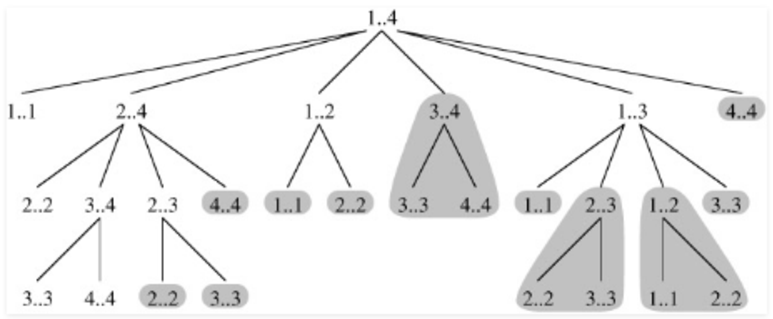
\includegraphics[width=0.7\textwidth]{Images/figGFGDPSet8MatChainMult}
\label{figGFGDPSet8MatChainMult}
\end{figure}

Since same suproblems are called again, this problem has Overlapping
Subprolems property. So Matrix Chain Multiplication problem has both
properties (see \pagecref{secGFGDPSet1OverlapSubprob} and
\pagecref{secGFGDPSet2OptimalSubstruct}) of a dynamic programming problem.
Like other typical Dynamic Programming(DP) problems, recomputations of same
subproblems can be avoided by constructing a temporary array $m[][]$ in
bottom up manner.

\rrheader{Dynamic Programming Solution}

Following is C/C++ implementation for Matrix Chain Multiplication problem
using Dynamic Programming.
\begin{lstlisting}[style=raycppnewsnippet]
// See the Cormen book for details of the following algorithm
#include<stdio.h>
#include<limits.h>
 
// Matrix Ai has dimension p[i-1] x p[i] for i = 1..n
int MatrixChainOrder(int p[], int n)
{
  /* For simplicity of the program, one extra row and one
     extra column are allocated in m[][].  0th row and 0th
     column of m[][] are not used */
  int m[n][n];
 
  int i, j, k, L, q;
 
  /* m[i,j] = Minimum number of scalar multiplications needed
     to compute the matrix A[i]A[i+1]...A[j] = A[i..j] where
     dimension of A[i] is p[i-1] x p[i] */
 
  // cost is zero when multiplying one matrix.
  for (i=1; i<n; i++)
    m[i][i] = 0;
 
  // L is chain length.
  for (L=2; L<n; L++)
  {
    for (i=1; i<n-L+1; i++)
    {
      j = i+L-1;
      m[i][j] = INT_MAX;
      for (k=i; k<=j-1; k++)
      {
        // q = cost/scalar multiplications
        q = m[i][k] + m[k+1][j] + p[i-1]*p[k]*p[j];
        if (q < m[i][j])
          m[i][j] = q;
      }
    }
  }
  return m[1][n-1];
}

int main()
{
    int arr[] = {1, 2, 3, 4};
    int size = sizeof(arr)/sizeof(arr[0]);
 
    printf("Minimum number of multiplications is %d ",
                       MatrixChainOrder(arr, size));
 
    getchar();
    return 0;
}
\end{lstlisting}
Output:
\begin{lstlisting}[style=rayio]
Minimum number of multiplications is 18
\end{lstlisting}
\rrhl{Time Complexity:} $\comBigOh{n^3}$\\
\rrhl{Auxiliary Space:} $\comBigOh{n^2}$

Printing brackets in Matrix Chain Multiplication Problem, see
\pagecref{secGFGDPPrintMatChainMult}.

Please write comments if you find anything incorrect, or you want to share
more information about the topic discussed above.

\subsection{Printing brackets in Matrix Chain Multiplication Problem
  \label{secGFGDPPrintMatChainMult}}

\url{http://www.geeksforgeeks.org/printing-brackets-matrix-chain-multiplication-problem}

\textbf{Difficulty: 4.4}

Given a sequence of matrices, find the most efficient way to multiply these
matrices together. The problem is not actually to perform the
multiplications, but merely to decide in which order to perform the
multiplications.

We have many options to multiply a chain of matrices because matrix
multiplication is associative. In other words, no matter how we parenthesize
the product, the result will be the same. For example, if we had four
matrices A, B, C, and D, we would have:
\begin{lstlisting}[style=raygeneric]
    (ABC)D = (AB)(CD) = A(BCD) = ....
\end{lstlisting}
However, the order in which we parenthesize the product affects the number
of simple arithmetic operations needed to compute the product, or the
efficiency. For example, suppose $A$ is a $10\times30$ matrix, $B$ is a
$30\times5$ matrix, and $C$ is a $5\times60$ matrix. Then,
\begin{equation*}
(AB)C=(10\times30\times5)+(10\times5\times60)=1500+3000=4500
\text{ operations}
\end{equation*}
\begin{equation*}
A(BC)=(30\times5\times60)+(10\times30\times60)=9000+18000=27000 
\text{ operations}.
\end{equation*}
Clearly the first parenthesization requires less number of operations.

Given an array $p[]$ which represents the chain of matrices such that the
$i$th matrix $A_i$ is of dimension $p[i-1]\times p[i]$. We need to write a
function $MatrixChainOrder()$ that should return the minimum number of
multiplications needed to multiply the chain.
\begin{lstlisting}[style=raygeneric]
  Input:  p[] = {40, 20, 30, 10, 30}  
  Output: Optimal parenthesization is  ((A(BC))D)
          Optimal cost of parenthesization is 26000
  There are 4 matrices of dimensions 40x20, 20x30, 30x10 and 10x30.
  Let the input 4 matrices be A, B, C and D.  The minimum number of 
  multiplications are obtained by putting parenthesis in following way
  (A(BC))D --> 20*30*10 + 40*20*10 + 40*10*30

  Input: p[] = {10, 20, 30, 40, 30} 
  Output: Optimal parenthesization is (((AB)C)D)
          Optimal cost of parenthesization is 30000
  There are 4 matrices of dimensions 10x20, 20x30, 30x40 and 40x30. 
  Let the input 4 matrices be A, B, C and D.  The minimum number of 
  multiplications are obtained by putting parenthesis in following way
  ((AB)C)D --> 10*20*30 + 10*30*40 + 10*40*30

  Input: p[] = {10, 20, 30}  
  Output: Optimal parenthesization is (AB)
          Optimal cost of parenthesization is 6000
  There are only two matrices of dimensions 10x20 and 20x30. So there 
  is only one way to multiply the matrices, cost of which is 10*20*30
\end{lstlisting}
This problem is mainly an extension of previous post
\pagecref{secGFGDPSet8MatChainMult}. In the previous post, we have discussed
algorithm for finding optimal cost only. Here we need print parenthssization
also.

\textbf{\rrgreen{Recommended: Please try your approach first, before moving
    on to the solution.}}

\RayNotesBegin

How about, we store the split point in another table, say $brkt[][]$. Let's
play with the example we have been using:
\begin{lstlisting}[style=raygeneric]
        0  1  2  3  4
p[] = [40,20,30,10,30] -> A1,A2,A3,A4

Table m:
j 0|1|2|3|4
i ---------
0| | | | | |
1| |1|2|3|4|
2| | |1|2|3|
3| | | |1|2|
4| | | | |1|

                1  2 3   4
The paren is: ((A1(A2A3))A4)
This means that 
brkt[1,4] = 3
  brkt[1,3] = 1 (left)
    brkt[1,1] = A1 (left)
    brkt[2,3] = 2 (right)
      brkt[2,2] = A2 (left)
      brkt[3,3] = A3 (right)
  brkt[4,4] = A4 right(right)
\end{lstlisting}
This clearly has a recursive structure, and we know that the base case is
when $i==j$, where we just output the matrix name (i.e. $A1$, $A2$, etc...). 
And before each call, we wrap it in brackets.
So the pseudocode would be something like
\begin{lstlisting}[style=pseudostyle,numbers=none]
printParens(brkt[][],i,j)
{
  if(i==j)
  {
    print "Ai"
  }
  else
  {
    print "("
    printParens(brkt,i,brkt[i,j])
    printParens(brkt,brkt[i,j]+1,j)
    print ")"
  }
}
\end{lstlisting}
Now let's code this up!

Code found in \path{src/DynamicProgramming/rrrGFGDPSet8MatChainMult.cpp}
\begin{lstlisting}[style=raycppnewsnippet]
void printParen(vector<vector<int>>&s, int i, int j)
{
  if(i==j)
  {
    cout << "A" << i;
  }
  else
  {
    cout << "(";
    printParen(s,i,s[i][j]);
    printParen(s,s[i][j]+1,j);
    cout << ")";
  }
}

// Matrix Ai has dimension p[i-1]xp[i] for i=1..n
//
//        0  1  2  3  4
//p[] = [40,20,30,10,30] -> A1,A2,A3,A4
//
//Table m:
//j 0|1|2|3|4
//i ---------
//0| | | | | |
//1| |1|2|3|4|
//2| | |1|2|3|
//3| | | |1|2|
//4| | | | |1|
//
//Table m's entries in the above represent the length, it depicts how the
//below algorithm fills in m, i.e. m[i,j] = i implies that i==j and we're 
//dealing with a matrix mult. of length 1, i.e. one matrix. These are NOT 
//the actual values of m. The actual values of m is the min. flops required
//to perform the mult. of chain length j-i+1.
void matChainMultDP(vector<int>& p)
{
  // length of p, so n-1 is the number of matrices to multiply.
  auto n = static_cast<int>(p.size());

  // Base case: i==j, chain of length 1, so there is no multiplication. We
  // would fill the diagonal entries with 0, but this is already done as 
  // part of the initialization.
  vector<vector<int>>m(n,vector<int>(n,0));
  
  // Used to record the split
  vector<vector<int>>s(n,vector<int>(n,0));

  // Loop from length of 2 to n-1
  for(int l=2; l<n; ++l)
  {
    // Loop down the matrix m.
    for(int i = 1; i < n-l+1; ++i)
    {
      // Calculate the j entries such that j-i+1=l.
      int j = l+i-1;

      // Set number of flops in m to max(), then we can minimize it.
      m[i][j] = std::numeric_limits<int>::max();

      // Loop through all possible splits.
      for(int k=i; k < j; ++k)
      {
        int q = p[i-1]*p[k]*p[j] // Top level mult.
                +m[i][k]         // min flops of left section
                +m[k+1][j];      // min flops of right section

        // Does this give a smaller flop count then a previous split?
        if(q<m[i][j])
        {
          m[i][j] = q;
          s[i][j] = k;
        }
      }
    }
  }
  
  cout << "Optimal flops: " << m[1][n-1] << '\n'
       << "With parens: ";
  printParen(s,1,n-1);
  cout << '\n';
}
\end{lstlisting}

\RayNotesEnd

\textbf{\rrgreen{Back to geeksforgeeks solution.}}

The idea is to store optimal break point for every subexpression $(i,j)$ in
a 2D array $bracket[n][n]$. Once we have bracket array us constructed, we
can print parenthesization using below code.
\begin{lstlisting}[style=raycppnewsnippet]
// Prints parenthesization in subexpression (i, j)
printParenthesis(i, j, bracket[n][n], name)
{
  // If only one matrix left in current segment
  if (i == j)
  {
    print name;
    name++;
    return;
  }

  print "(";

  // Recursively put brackets around subexpression
  // from i to bracket[i][j].
  printParenthesis(i, bracket[i][j], bracket, name);

  // Recursively put brackets around subexpression
  // from bracket[i][j] + 1 to j.
  printParenthesis(bracket[i][j]+1, j, bracket, name);

  print ")";
}
\end{lstlisting}

Below is C++ implementation of above steps.
\begin{lstlisting}[style=raycppnewsnippet]
// C++ program to print optimal parenthesization
// in matrix chain multiplication.
#include<bits/stdc++.h>
using namespace std;
 
// Function for printing the optimal
// parenthesization of a matrix chain product
void printParenthesis(int i, int j, int n,
                      int *bracket, char &name)
{
  // If only one matrix left in current segment
  if (i == j)
  {
    cout << name++;
    return;
  }
 
  cout << "(";
 
  // Recursively put brackets around subexpression
  // from i to bracket[i][j].
  // Note that "*((bracket+i*n)+j)" is similar to
  // bracket[i][j]
  printParenthesis(i, *((bracket+i*n)+j), n,
                   bracket, name);
 
  // Recursively put brackets around subexpression
  // from bracket[i][j] + 1 to j.
  printParenthesis(*((bracket+i*n)+j) + 1, j,
                   n, bracket, name);
  cout << ")";
}

// Matrix Ai has dimension p[i-1] x p[i] for i = 1..n
// Please refer below article for details of this
// function
// https://goo.gl/k6EYKj
void matrixChainOrder(int p[], int n)
{
  /* For simplicity of the program, one extra
     row and one extra column are allocated in
      m[][]. 0th row and 0th column of m[][]
      are not used */
  int m[n][n];
 
  // bracket[i][j] stores optimal break point in
  // subexpression from i to j.
  int bracket[n][n];
 
  /* m[i,j] = Minimum number of scalar multiplications
  needed to compute the matrix A[i]A[i+1]...A[j] =
  A[i..j] where dimension of A[i] is p[i-1] x p[i] */
 
  // cost is zero when multiplying one matrix.
  for (int i=1; i<n; i++)
    m[i][i] = 0;
 
  // L is chain length.
  for (int L=2; L<n; L++)
  {
    for (int i=1; i<n-L+1; i++)
    {
      int j = i+L-1;
      m[i][j] = INT_MAX;
      for (int k=i; k<=j-1; k++)
      {
        // q = cost/scalar multiplications
        int q = m[i][k] + m[k+1][j] + p[i-1]*p[k]*p[j];
        if (q < m[i][j])
        {
          m[i][j] = q;
 
          // Each entry bracket[i,j]=k shows
          // where to split the product arr
          // i,i+1....j for the minimum cost.
          bracket[i][j] = k;
        }
      }
    }
  }
  // The first matrix is printed as 'A', next as 'B',
  // and so on
  char name = 'A';
 
  cout << "Optimal Parenthesization is : ";
  printParenthesis(1, n-1, n, (int *)bracket, name);
  cout << "nOptimal Cost is : " << m[1][n-1];
}

// Driver code
int main()
{
  int arr[] = {40, 20, 30, 10, 30};
  int n = sizeof(arr)/sizeof(arr[0]);
  matrixChainOrder(arr, n);
  return 0;
}
\end{lstlisting}

Output:
\begin{lstlisting}[style=rayio]
Optimal Parenthesization: ((A(BC))D)
Minimum Cost of Multiplication: 26000
\end{lstlisting}
\rrhl{Time Complexity:} $O(n^3)$\\
\rrhl{Auxiliary Space:} $O(n^2)$

%%%%%%%%%%%%%%%%%%%%%%%%%%%%%%%%%%%%%%%%%%%%%%%%%%%%%%%%%%%%%%%%%%%%%%%%%%%%
%%%%%%%%%%%%%%%%%%%%%%%%%%%%%%%%%%%%%%%%%%%%%%%%%%%%%%%%%%%%%%%%%%%%%%%%%%%%
%%%%%%%%%%%%%%%%%%%%%%%%%%%%%%%%%%%%%%%%%%%%%%%%%%%%%%%%%%%%%%%%%%%%%%%%%%%%

\section{Dynamic Programming | Set 9 (Binomial Coefficient)
  \label{secGFGDPSet9BinomCoeff}}

\url{http://www.geeksforgeeks.org/dynamic-programming-set-9-binomial-coefficient}

\textbf{Difficulty: 2.5}

Following are common definition of Binomial Coefficients.
\begin{enumerate}[label=\textbf{\arabic*.}]
\item A binomial
  coefficient\footnote{\url{https://en.wikipedia.org/wiki/Binomial\_coefficient}}
  $C(n,k)$ can be defined as the coefficient of $X^k$ in the expansion of
  $(1+X)^n$.
\item A binomial coefficient $C(n,k)$ also gives the number of ways,
  disregarding order, that $k$ objects can be chosen from among $n$ objects;
  more formally, the number of $k$-element subsets (or $k$-combinations
  \rrblue{(order does not matter in $k-$combinations. For a permutation,
    order matters)}) of an $n$-element set.
\end{enumerate}

\rrheader{The Problem}

Write a function that takes two parameters $n$ and $k$ and returns the value
of Binomial Coefficient $C(n,k)$. For example, your function should return
$6$ for $n=4$ and $k=2$, and it should return $10$ for $n=5$ and $k = 2$.

\textbf{\rrgreen{Recommended: Please try your approach first, before moving
    on to the solution.}}

\RayNotesBegin

Err... isn't the binomial coefficient formula:
\begin{equation*}
\binom{n}{k} = \frac{n!}{(n-k)!k!}
\end{equation*}
Let's see, $C(n=5,k=2) = 5!/(3!2!) = 10$

However, if we \emph{had} to use dynamic programming, then we'll need to
come up with a recursive definition which exhibits an optimal substructure
property, and that there are overlapping subproblem.

From the wikipedia article, the recursive formula is
\begin{mdframed}[style=mdfNOTE,
frametitle={Recursive formula from wikipedia}]
\begin{equation*}
\binom{n}{k} = \binom{n-1}{k-1}+\binom{n-1}{k}
\text{ for all integers }n,k:1\leq k \leq n-1,
\end{equation*}
with initial/boundary values
\begin{equation*}
\binom{n}{0} = \binom{n}{n} = 1 \text{ for all integers }n\geq 0.
\end{equation*}
The formula follows from considering the set $\brce*{1,2,\ldots,n}$ and
counting separately
\begin{enumerate}[label=\textbf{\alph*.}]
\item the $k$-element groupings that include a particular set element, say
  ``$i$'', in every group (since ``$i$'' is already chosen to fill one spot
  in every group, we need only choose $k-1$ from the remaining $n-1$) and
\item all the $k$-groupings that don't include ``$i$''; 
\end{enumerate}
this enumerates all the possible $k$-combinations of $n$ elements. It also
follows from tracing the contributions to $X^k$ in $(1+x)^{n-1}(x+x)$. As
there is zero $x^{n+1}$ or $x^{-1}$ in $(1+x)^n$, one might extend the
definition beyond the above boundaries o include $\binom{n}{k}=0$ when
either $k>n$ or $k<0$. This recursive formula then allows the construction
of Pascal's triangle, surrounded by white spaces where the zero, or the
trivial coefficients, would be.
\end{mdframed}

I'm not quite sure that the above means, however the recursive formula can
be seen from Pascal's triangle. However, I get ``It also follows from
tracing the contributions to $X^k$ in $(1+x)^{n-1}(x+x)$.'' Let's look at
Pascal's Triangle:

\begin{tabular}{cccccccccccc}
$n=0$ &&&&&1&&&&    &$(x+y)^0=$&$1$\\
$n=1$ &&&&1&&1&&&   &$(x+y)^1=$&$x+y$\\
$n=2$ &&&1&&2&&1&&  &$(x+y)^2=$&$x^2+2xy+y^2$\\
$n=3$ &&1&&3&&3&&1& &$(x+y)^3=$&$x^3+3x^2y+3xy^2+y^3$\\
$n=4$ &1&&4&&6&&4&&1&$(x+y)^4=$&$x^4+4x^3y+6x^2y^2+4xy^3+y^4$
\end{tabular}

Look how Pascal's Triangle is formed. It's formed by adding the adjacent
digits on the previous row. But we also know that the coefficients of the
binomial are:

\begin{tabular}{cccccccccccc}
$n=0$ &&&&&$\binom{0}{0}$&&&&    &&$1$\\
$n=1$ &&&&$\binom{1}{1}$&&$\binom{1}{0}$&&&   &&$x+y$\\
$n=2$ &&&$\binom{2}{2}$&&$\binom{2}{1}$&&$\binom{2}{0}$&&  &&$x^2+2xy+y^2$\\
$n=3$ &&$\binom{3}{3}$&&$\binom{3}{2}$&&$\binom{3}{1}$&&$\binom{3}{0}$& &&$x^3+3x^2y+3xy^2+y^3$\\
$n=4$
&$\binom{4}{4}$&&$\binom{4}{3}$&&$\binom{4}{2}$&&$\binom{4}{1}$&&$\binom{4}{0}$&&$x^4+4x^3y+6x^2y^2+4xy^3+y^4$
\end{tabular}

As you can see, take $\binom{4}{2}$ for example, the coefficient is clearly
the result of $\binom{3}{2}+\binom{3}{1}$. Of course, you can prove thus by
using the formula $\displaystyle\binom{n}{k} = \frac{n!}{(n-k)!k!}$ and
proving the identity
\begin{equation*}
\binom{n}{k} = \binom{n-1}{k}+\binom{n-1}{k-1}
\end{equation*}

\qasepline{}

Now we can use the recursive definition to do dynamic programming! Given
\begin{equation*}
C(n,k) = C(n-1,k)+C(n-1,k-1)
\end{equation*}
and initial/boundary conditions
\begin{equation*}
C(n,n) = C(n,0) = 1
\end{equation*}
So, let's code his up! Done, code found in:\\
\path{LeetCode/src/DynamicProgramming/rrrGFGDPSet9BinomCoeff.cpp}
\begin{lstlisting}[style=raycppnewsnippet]
unsigned BinomCoeff(unsigned n, unsigned k)
{
  if(k==n || k == 0) return 1;

  if(k>n || k<0) return 0;

  return BinomCoeff(n-1,k)+BinomCoeff(n-1,k-1);
}
void runBinomCoeff(unsigned n, unsigned k)
{
  cout << "C"<<n<<","<<k<<")="<<BinomCoeff(n,k) <<'\n';
}
\end{lstlisting}
Now, how do we do it bottom up? Simples:
\begin{enumerate}[label=\textbf{\arabic*.}]
\item as before, we need a structure to hold the results, let's call this
  $c$. It needs to be 2D because there are two state variables.
\item How do we fill this up? Well, let's do as we did the chain matrix
  mult. We start with a small example and fill in the base case, and see how
  we work up to the final cell.
\end{enumerate}

Let's do $C(n=4,k=3)$. So we have $c=$\\
\begin{tabular}{|c|c|c|c|c|}\hline
\diagbox{$n$}{$k$}&\textbf{0}&\textbf{1}&\textbf{2}&\textbf{3}\\\hline
\textbf{0}&&&&\\\hline 
\textbf{1}&&&&\\\hline
\textbf{2}&&&&\\\hline
\textbf{3}&&&&\\\hline
\textbf{4}&&&&\rrred{4}\\\hline
\end{tabular}\\
where $C(4,3)=4$ (in red) is where we want to get to. First we fill in the
base cases:\\
\begin{tabular}{|c|c|c|c|c|}\hline
\diagbox{$n$}{$k$}&\textbf{0}&\textbf{1}&\textbf{2}&\textbf{3}\\\hline
\textbf{0}&1&&&\\\hline 
\textbf{1}&1&1&&\\\hline
\textbf{2}&1&&1&\\\hline
\textbf{3}&1&&&1\\\hline
\textbf{4}&1&&&\rrred{4}\\\hline
\end{tabular}\\
Now look at the recursion
\begin{equation*}
C(n,k) = \underbrace{C(n-1,k)}_\text{top}+\underbrace{C(n-1,k-1)}_\text{top
left}
\end{equation*}
we know we simply have to loop from $i=2..n$ and $j=1..k-1$. Let's code this
up! Okay, done, this works.
\begin{lstlisting}[style=raycppnewsnippet]
//////////////////////////////////////////////////////////
unsigned BinomCoeffDP(unsigned n, unsigned k)
{
  // Make (n+1)x(k+1) table of 0's
  // we need +1 to account for the zero entry for when we do choose 0 out
  // of n, i.e. C(n,0) = 1.
  auto nrow = n+1;
  auto ncol = k+1;

  vector<vector<unsigned>> dp(nrow,vector<unsigned>(ncol,0));

  // Base case, set C(n,0) = 1, i.e. set the first column to 1's
  for(size_t i = 0; i < nrow; ++i)
  {
    dp[i][0]=1;
  }

  // base case: set C(n,n) to 1, i.e. set the diagonal entries to 1
  for(size_t j = 0; j < ncol; ++j)
  {
    dp[j][j]=1;
  }

  // Calculate binom coeff according to the recursive formula
  // dp[i,j] = dp[i-1,j-1]+dp[i-1,j]
  // See my notes for why I start i = 2 and j=1. It follows from a sketch of
  // dp with the boundary conditions filled only.
  for(size_t i = 2; i <= n; ++i)
  {
    for(size_t j = 1; j <= k; ++j)
    {
      dp[i][j] = dp[i-1][j-1]+dp[i-1][j];
    }
  }

  return dp[n][k];
}
\end{lstlisting}
Code found in:\\
\path{LeetCode/src/DynamicProgramming/rrrGFGDPSet9BinomCoeff.cpp}

\RayNotesEnd

\textbf{\rrgreen{Back to geeksforgeeks solution.}}

\rrheader{(1) Optimal Substructure}

The value of $C(n,k)$ can be recursively calculated using following standard
formula for Binomial Coefficients.
\begin{lstlisting}[style=raygeneric]
C(n, k) = C(n-1, k-1) + C(n-1, k)
C(n, 0) = C(n, n) = 1
\end{lstlisting}
Following is a simple recursive implementation that simply follows the
recursive structure mentioned above.
\begin{lstlisting}[style=raycppnewsnippet]
// A Naive Recursive Implementation
#include<stdio.h>
 
// Returns value of Binomial Coefficient C(n, k)
int binomialCoeff(int n, int k)
{
  // Base Cases
  if (k==0 || k==n)
    return 1;
 
  // Recur
  return  binomialCoeff(n-1, k-1) + binomialCoeff(n-1, k);
}
 
/* Driver program to test above function*/
int main()
{
    int n = 5, k = 2;
    printf("Value of C(%d, %d) is %d ", n, k, binomialCoeff(n, k));
    return 0;
}
\end{lstlisting}

\rrheader{(2) Overlapping Subproblems}

It should be noted that the above function computes the same subproblems
again and again. See the following recursion tree for $n = 5$ and $k = 2$.
The function $C(3,1)$ is called two times. For large values of $n$, there
will be many common subproblems.
\begin{lstlisting}[style=raygeneric]
                             C(5, 2)
                    /                      \
           C(4, 1)                           C(4, 2)
            /   \                          /           \
       C(3, 0)   C(3, 1)             C(3, 1)               C(3, 2)
                /    \               /     \               /     \
         C(2, 0)    C(2, 1)      C(2, 0) C(2, 1)          C(2, 1)  C(2, 2)
                   /        \              /   \            /    \
               C(1, 0)  C(1, 1)      C(1, 0)  C(1, 1)   C(1, 0)  C(1, 1)
\end{lstlisting}
Since same suproblems are called again, this problem has Overlapping
Subproblems property. So the Binomial Coefficient problem has both
properties (see this and this) of a dynamic programming problem. Like other
typical Dynamic Programming(DP) problems, re-computations of same
subproblems can be avoided by constructing a temporary array $C[][]$ in
bottom up manner. Following is Dynamic Programming based implementation.
\begin{lstlisting}[style=raycppnewsnippet]
// A Dynamic Programming based solution that uses table C[][] to
// calculate the Binomial Coefficient
#include<stdio.h>
 
// Prototype of a utility function that returns minimum of two integers
int min(int a, int b);
 
// Returns value of Binomial Coefficient C(n, k)
int binomialCoeff(int n, int k)
{
  int C[n+1][k+1];
  int i, j;
 
  // Caculate value of Binomial Coefficient in bottom up manner
  for (i = 0; i <= n; i++)
  {
    for (j = 0; j <= min(i, k); j++)
    {
      // Base Cases
      if (j == 0 || j == i)
        C[i][j] = 1;
 
      // Calculate value using previosly stored values
      else
        C[i][j] = C[i-1][j-1] + C[i-1][j];
    }
  }
    return C[n][k];
}

// A utility function to return minimum of two integers
int min(int a, int b)
{
  return (a<b)? a: b;
}
 
/* Drier program to test above function*/
int main()
{
  int n = 5, k = 2;
  printf ("Value of C(%d, %d) is %d ", n, k, binomialCoeff(n, k) );
  return 0;
}
\end{lstlisting}
Output:
\begin{lstlisting}[style=rayio]
Value of C[5][2] is 10
\end{lstlisting}

\noindent{}\rrhl{Time Complexity:} $\comBigOh{nk}$\\
\rrhl{Auxiliary Space:} $\comBigOh{nk}$\\

Following is a space optimized version of the above code. The following code
only uses $\comBigOh{k}$. Thanks to AK for suggesting this method.
\begin{lstlisting}[style=raycppnewsnippet]
// C++ program for space optimized Dynamic Programming
// Solution of Binomial Coefficient
#include<bits/stdc++.h>
using namespace std;
 
int binomialCoeff(int n, int k)
{
  int C[k+1];
  memset(C, 0, sizeof(C));

  C[0] = 1;  // nC0 is 1

  for (int i = 1; i <= n; i++)
  {
    // Compute next row of pascal triangle using
    // the previous row
    for (int j = min(i, k); j > 0; j--)
      C[j] = C[j] + C[j-1];
  }
  return C[k];
}
 
/* Driver program to test above function*/
int main()
{
  int n = 5, k = 2;
  printf ("Value of C(%d, %d) is %d ",
          n, k, binomialCoeff(n, k) );
  return 0;
}
\end{lstlisting}
Output:
\begin{lstlisting}[style=rayio]
Value of C[5][2] is 10
Time Complexity: O(n*k)
Auxiliary Space: O(k)
\end{lstlisting}
Explanation:
\begin{lstlisting}[style=raygeneric]
1==========>> n = 0, C(0,0) = 1
1-1========>> n = 1, C(1,0) = 1, C(1,1) = 1
1-2-1======>> n = 2, C(2,0) = 1, C(2,1) = 2, C(2,2) = 1
1-3-3-1====>> n = 3, C(3,0) = 1, C(3,1) = 3, C(3,2) = 3, C(3,3)=1
1-4-6-4-1==>> n = 4, C(4,0) = 1, C(4,1) = 4, C(4,2) = 6, C(4,3)=4, C(4,4)=1
\end{lstlisting}
So here every loop on $i$, builds $i$th row of pascal triangle, using
$(i-1)$th row

At any time, every element of array $C$ will have some value (ZERO or more)
and in next iteration, value for those elements comes from previous
iteration.

In statement,
\begin{lstlisting}[style=raycppnewsnippet]
C[j] = C[j] + C[j-1]
\end{lstlisting}
Right hand side represents the value coming from previous iteration (A row
of Pascal's triangle depends on previous row). Left Hand side represents the
value of current iteration which will be obtained by this statement.
\begin{lstlisting}[style=raygeneric]
Let's say we want to calculate C(4, 3), 
i.e. n=4, k=3:

All elements of array C of size 4 (k+1) are
initialized to ZERO.

i.e. C[0] = C[1] = C[2] = C[3] = C[4] = 0;
Then C[0] is set to 1

For i = 1:
C[1] = C[1] + C[0] = 0 + 1 = 1 ==>> C(1,1) = 1

For i = 2:
C[2] = C[2] + C[1] = 0 + 1 = 1 ==>> C(2,2) = 1
C[1] = C[1] + C[0] = 1 + 1 = 2 ==>> C(2,2) = 2

For i=3:
C[3] = C[3] + C[2] = 0 + 1 = 1 ==>> C(3,3) = 1
C[2] = C[2] + C[1] = 1 + 2 = 3 ==>> C(3,2) = 3
C[1] = C[1] + C[0] = 2 + 1 = 3 ==>> C(3,1) = 3

For i=4:
C[4] = C[4] + C[3] = 0 + 1 = 1 ==>> C(4,4) = 1
C[3] = C[3] + C[2] = 1 + 3 = 4 ==>> C(4,3) = 4
C[2] = C[2] + C[1] = 3 + 3 = 6 ==>> C(4,2) = 6
C[1] = C[1] + C[0] = 3 + 1 = 4 ==>> C(4,1) = 4

C(4,3) = 4 is would be the answer in our example.
\end{lstlisting}
See this for Space and time efficient Binomial Coefficient
\url{http://www.geeksforgeeks.org/space-and-time-efficient-binomial-coefficient/}

RRRTODO

%%%%%%%%%%%%%%%%%%%%%%%%%%%%%%%%%%%%%%%%%%%%%%%%%%%%%%%%%%%%%%%%%%%%%%%%%%%%
%%%%%%%%%%%%%%%%%%%%%%%%%%%%%%%%%%%%%%%%%%%%%%%%%%%%%%%%%%%%%%%%%%%%%%%%%%%%
%%%%%%%%%%%%%%%%%%%%%%%%%%%%%%%%%%%%%%%%%%%%%%%%%%%%%%%%%%%%%%%%%%%%%%%%%%%%

\section{Dynamic Programming | Set 10 (0-1 Knapsack Problem)
  \label{secGFGDPSet10Knapsack01Prob}}

\url{http://www.geeksforgeeks.org/knapsack-problem}

\textbf{Difficulty: 3.3}

Given weights and values of $n$ items, put these items in a knapsack of
capacity $W$ to get the maximum total value in the knapsack. In other words,
given two integer arrays $val[0..n-1]$ and $wt[0..n-1]$ which represent
values and weights associated with $n$ items respectively. Also given an
integer $W$ which represents knapsack capacity, find out the \textbf{maximum
  value} subset of $val[]$ such that \textbf{sum of the weights} of this
subset is smaller than or equal to $W$. You cannot break an item, either
pick the complete item, or don't pick it (0-1 property).

\begin{figure}
\centering
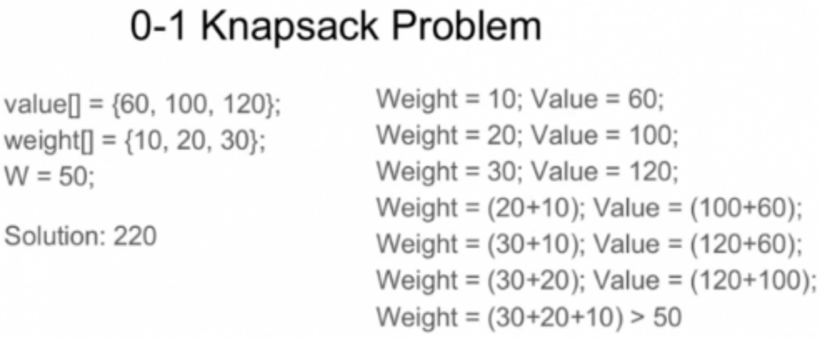
\includegraphics[width=0.7\textwidth]{Images/figGFGDPSet10Knapsack}
\end{figure}

\textbf{\rrgreen{Recommended: Please try your approach first, before moving
    on to the solution.}}

\RayNotesBegin

This is similar to the integer partitioning problem seen in
\pagecref{secGFGDPSet7CoinChange}. In the integer partitioning problem, the
weights and the values have a 1-1 (one to one) mapping. I.e. a value of $5$
has weight $5$. Here, is a more general case where the mapping is defined by
$wt[]$. Thus, we take a similar approach. For each partitioning, we either
use $val[i]$ or we don't. And we must calculate the max weight possible.

Let's start at the right-most val and work backwards, and take a look at
what happens in the two cases:
\begin{lstlisting}[style=raygeneric]
maxWeight(val[],wt[],W,i) = max(maxWeight(val[],wt[],W-wt[i],i  )+val[i]
                                maxWeight(val[],wt[],W,     ,i-1)       )
\end{lstlisting}
If we do use the $val[i]$, then we have the contribution $+val[i]$ to the
knapsack, the resulting subproblem must be of weight $W:=W-wt[i]$. But we're
still using all the values and weights, so $i$ does not change.

If we do not use the weight, in the resulting subproblem, $W$ does not
change, but we reduce the number of weights by 1, hence $i:=i-1$.

This will generate all possible combinations. To see this, consider a small
example: Let $val[]=\brce*{60,100,120}$, $wt[]=\brce*{10,20,30}$ and $W=220$.
Consider what happens if we keep going down the left side of \ctt{max}:
\begin{lstlisting}[style=raygeneric, numbers=left]
       maxWeight(val[],wt[],50,2)
(left) maxWeight(val[],wt[],20,2)+120
(left) maxWeight(val[],wt[],-10,2) END
\end{lstlisting}
This leads to a single val of $120$ with weight $30$ in the bag. But at line
2, instead of going down the left path, if we go down the right path, we
have 
\begin{lstlisting}[style=raygeneric, numbers=left]
       maxWeight(val[],wt[],50,2)
(left) maxWeight(val[],wt[],20,2)+120
(right)maxWeight(val[],wt[],20,1)
(left) maxWeight(val[],wt[],0 ,1)+100
\end{lstlisting}
So we end up with a solution of 220 with $W=0$, this is optimal. What
happens if we keep going to the right?
\begin{lstlisting}[style=raygeneric, numbers=left]
       maxWeight(val[],wt[],50,2)
(right)maxWeight(val[],wt[],50,1)
(right)maxWeight(val[],wt[],50,0)
(right)maxWeight(val[],wt[],50,-1) END
\end{lstlisting}
So we end up with a solution of 0 with $W=50$, this is not a good solution.
However, if in line 3, we take the left path, then we have
\begin{lstlisting}[style=raygeneric, numbers=left]
       maxWeight(val[],wt[],50,2)
(right)maxWeight(val[],wt[],50,1)
(right)maxWeight(val[],wt[],50,0)
(left) maxWeight(val[],wt[],40,0)+60
(left) maxWeight(val[],wt[],30,0)+60
(left) maxWeight(val[],wt[],20,0)+60
(left) maxWeight(val[],wt[],10,0)+60
(left) maxWeight(val[],wt[], 0,0)+60
\end{lstlisting}
So we end up with a solution of 300 with $W=0$, this is even better, and
all we've used are $val=60, wt=10$.

\qasepline{}

The above solution is for when we can pick an item multiple times. If we
cannot pick an item multiple times, then we need a simple modification:
\begin{lstlisting}[style=raygeneric]
maxWeight(val[],wt[],W,i) = max(maxWeight(val[],wt[],W-wt[i],i-1)+val[i]
                                maxWeight(val[],wt[],W,     ,i-1)       )
\end{lstlisting}
On the left path, by adding $i-1$ instead of just $i$, we ensure that once
the item is used, we cannot re-use it. 

Initial and boundary conditions: Since there are two state variables,
logically, there must be four boundary conditions.
\begin{itemize}%[noitemsep,topsep=0pt]
\item If $W=0$, we have no more room, we return $0$ immediately.
\item If $i < 0$, we have no more items, return $0$ immediately.
\item If $W-wt[i]<0$, then we cannot take the weight $wt[i]$ off, we can
  only take the right path (try with a lower weighted item):
\begin{lstlisting}[style=pseudostyle]
if(wt[i]>W)
  return maxWeight(val[],wt[],W,i-1) // go to the right path
\end{lstlisting}
\item Else, we're good to continue taking the max weight:
\begin{lstlisting}[style=pseudostyle]
return max(maxWeight(val[],wt[],W-wt[i],i-1)+val[i],
           maxWeight(val[],wt[],W      ,i-1)        )
\end{lstlisting}
\end{itemize}
Now let's code this up. Aside: I've never known whether I should using a
variable, say $n$, to represent the number of something or whether I could
be using it in terms of an index for a vector. For example:
\begin{lstlisting}[style=raycppnewsnippet]
// i is the number of items, so we need to index with i-1
// i.e. we start counting from 1
void foo(vector<int> v, int i)
{
  vector<int> bar(i);
  auto q = v[i-1];
}
// i is what we use to index a vector, so the caller has to remember to 
// subtract one. I.e. we start counting from 0
void foo(vector<int> v, int i)
{
  vector<int> bar(i+1);
  auto q = v[i];
}
\end{lstlisting}
The former is based 1, the latter is based 0. I'll stick with based 1 for
now since it's more natural. I can hope with fiddling with $-1$ within the
function. In light of this, we have to change our boundary conditions:
\begin{itemize}%[noitemsep,topsep=0pt]
\item If $W=0$, we have no more room, we return $0$ immediately.
\item If $n=0$, we have no more items, return $0$ immediately.
\item If $W-wt[i]<0$, then we cannot take the weight $wt[i]$ ff, we can only
  take the right path (try with a lower weighted item):
\begin{lstlisting}[style=raycppnewsnippet]
if(wt[i]>W)
  return maxWeight(val[],wt[],W,i-1) // go down the right path
\end{lstlisting}
\item Else, we're good to continue taking the max weight:
\begin{lstlisting}[style=raycppnewsnippet]
return max(maxWeight(val[],wt[],W-wt[@Ri-1@],i-1)+val[@Ri-1@],
           maxWeight(val[],wt[],W        ,i-1)          )
\end{lstlisting}
\end{itemize}
Now let's finally code this up. Code found in\\
\path{src/DynamicProgramming/rrrGFGDPSet10Knapsack.cpp}
\begin{lstlisting}[style=raycppnewsnippet]
// Returns the maximum value that can be put in a knapsack of capacity W
template<typename T>
auto knapsack(const vector<T>& val, const vector<T>& wt, 
              const T W, const int n)->T
{
  if(W == 0)
    return 0;
  if(n == 0)
    return 0;

  if(wt[n-1]>W)
    return 0;

  return std::max(knapsack(val,wt,W-wt[n-1],n-1)+val[n-1],
                  knapsack(val,wt,W        ,n-1)          );
}
int main()
{
  {
    vector<int> val{60,100,120};
    vector<int> wt{10,20,30};
    int W = 50;
    int n = val.size();
    cout << knapsack(val,wt,W,n) << '\n';
  }
  return 0;
}
\end{lstlisting}
Now let's do some DP. We know that the state variables are $W$ and $n$, so
let's first define a table to store the results for subproblems:
$dp[W+1][n+1]$,
i.e. this is a $(W+1)\times (n+1)$, where the rows represents all possible
weights (including $0$, hence the $+1$), and the column represents all
possible indices to index the current weight and value. From the recursion:
\begin{lstlisting}[style=raycppnewsnippet]
return max(maxWeight(val[],wt[],@bfW-wt[i-1]@,@bfi-1@)+val[i-1],
           maxWeight(val[],wt[],@bfW@        ,@bfi-1@)          )
\end{lstlisting}
we see that \ctt{dp[i,j]} only depends on the solutions in the top left cell
of $dp$ (due to $(W-wt[i-1],i-1)$) and to the cell on the left (due to
$(W,i-1)$). Thus it's okay to fill $dp$ in row major order from left to
right.

Base cases:\\
\begin{tabular}{|c|c|c|c|c|c|c|}\hline
\diagbox{$W$}{$n$}&\textbf{0}&\textbf{1}&\textbf{2}&\textbf{3}&\textbf{...}&\textbf{n}\\\hline
\textbf{0}&0&0&0&0&0&0\\\hline 
\textbf{1}&0&&&&&\\\hline
\textbf{2}&0&&&&&\\\hline
\textbf{3}&0&&&&&\\\hline
\textbf{4}&0&&&&&\\\hline
\textbf{...}&0&&&&&\\\hline
\textbf{W}&0&&&&&\rrred{ans}\\\hline
\end{tabular}\\
The above table covers the base cases $W=0$ or $n=0$. For the recursive
cases, note that $dp[i,j]$ depends on $dp[i-wt[i],j-1]$ and $dp[i,j-1]$. The
cell $dp[i-wt[i],j-1]$ may not exist if $i-wt[i]<0$, but $dp[i,j-1]$ is
always guaranteed to exist since we only go one to the left, so at most we
hit the base case for $n=0$. Thus, we have to check if $wt[i]>i$ and only
include the solution to the left if so.

Done, code found in \path{src/DynamicProgramming/rrrGFGDPSet10Knapsack.cpp}
\begin{lstlisting}[style=raycppnewsnippet]
template<typename T>
auto knapsackDP(const vector<T>& val, const vector<T>& wt, int W)-> T
{
  using vecsz_t = decltype(val.size());
  // number of items
  auto n = val.size();

  // table for tabulation, +1 for zero entry
  // Note that this also covers the base cases dp[i,j]=0 for i=0 || j=0
  // ALSO NOTE: that when referring to dp, it is "based 1", i.e. if we have 
  // three items,
  // val[]={60, 100, 120}
  // wt[] ={10, 20,  30}
  // Then to refer to the first item, we do val[0], but to refer to the 
  // first item in dp, we do dp[1][1]... hope this makes sense.
  // Also, treat dp as if you were passing state params to a function. So 
  // in the recursive case, it is base 1, so we do it here also.
  // But when referring to the current val, we need to use val[j-1] instead 
  // of just val[j]. Also note that wt is indexed with j, NOT by i which 
  // loops over all weight values.
  vector<vector<T>> dp(W+1,vector<T>(n+1,T{0}));

  for(vecsz_t i = 0; i <= W; ++i)
  {
    for(vecsz_t j = 0; j <= n; ++j)
    {
      if(wt[j-1]>i)
      {
        dp[i][j] = dp[i][j-1];
      }
      else
      {
        dp[i][j] = std::max(dp[i-wt[j-1]][j-1] + val[j-1],
                            dp[i][j-1]);
      }
    }
  }

  return dp[W][n];
}
\end{lstlisting}
I works, let's see the GFG solution.

\RayNotesEnd

\textbf{\rrgreen{Back to geeksforgeeks solution.}}

A simple solution is to consider all subsets of items and calculate the
total weight and value of all subsets. Consider the only subsets whose total
weight is smaller than \rrblue{(or equal to)} $W$. From all such subsets,
pick the maximum value subset.

\rrheader{(1) Optimal Substructure:}

To consider all subsets of items, there can be two cases for every item:
\textbf{(1)} the item is included in the optimal subset, \textbf{(2)} not
included in the optimal set.

Therefore, the maximum value that can be obtained from $n$ items is max of
following two values.
\begin{enumerate}[label=\textbf{\arabic*.}]
\item Maximum value obtained by $n-1$ items and $W$ weight (excluding $n$th
  item).
\item Value of $n$th item plus maximum value obtained by $n-1$ items and $W$
  minus weight of the $n$th item (including $n$th item).
\end{enumerate}

If weight of $n$th item is greater than $W$, then the $n$th item cannot be
included and case 1 is the only possibility.

\rrheader{(2) Overlapping Subproblems}

Following is recursive implementation that simply follows the recursive
structure mentioned above.
\begin{lstlisting}[style=raycppnewsnippet]
/* A Naive recursive implementation of 0-1 Knapsack problem */
#include<stdio.h>
 
// A utility function that returns maximum of two integers
int max(int a, int b) { return (a > b)? a : b; }
 
// Returns the maximum value that can be put in a knapsack of capacity W
int knapSack(int W, int wt[], int val[], int n)
{
  // Base Case
  if (n == 0 || W == 0)
    return 0;
 
  // If weight of the nth item is more than Knapsack capacity W, then
  // this item cannot be included in the optimal solution
  if (wt[n-1] > W)
    return knapSack(W, wt, val, n-1);
 
  // Return the maximum of two cases: 
  // (1) nth item included 
  // (2) not included
  else return max( val[n-1] + knapSack(W-wt[n-1], wt, val, n-1),
                   knapSack(W, wt, val, n-1)
                 );
}
 
// Driver program to test above function
int main()
{
  int val[] = {60, 100, 120};
  int wt[] = {10, 20, 30};
  int  W = 50;
  int n = sizeof(val)/sizeof(val[0]);
  printf("%d", knapSack(W, wt, val, n));
  return 0;
}
\end{lstlisting}
Output:
\begin{lstlisting}[style=rayio]
220
\end{lstlisting}
It should be noted that the above function computes the same subproblems
again and again. See the following recursion tree, $K(1,1)$ is being
evaluated twice. Time complexity of this na\"ive recursive solution is
exponential ($2^n$) \rrblue{(since either an item is included, or it's
  not)}.

In the following recursion tree, $K()$ refers to $knapSack()$.  The two
parameters indicated in the following recursion tree are $n$ and $W$.  The
recursion tree is for following sample inputs.  $wt[] = {1, 1, 1}$, $W = 2$,
$val[] = {10, 20, 30}$
\begin{lstlisting}[style=raygeneric]
                       K(3, 2)         ---------> K(n, W)
                   /            \ 
                 /                \               
            K(2,2)                  K(2,1)
          /       \                  /    \ 
        /           \              /        \
       K(1,2)      K(1,1)        K(1,1)     K(1,0)
       /  \         /   \          /   \
     /      \     /       \      /       \
K(0,2)  K(0,1)  K(0,1)  K(0,0)  K(0,1)   K(0,0)

Recursion tree for Knapsack capacity 2 units and 3 items of 1 unit weight.
\end{lstlisting}
Since suproblems are evaluated again, this problem has Overlapping
Subprolems property. So the 0-1 Knapsack problem has both properties (see
this and this) of a dynamic programming problem. Like other typical Dynamic
Programming(DP) problems, recomputations of same subproblems can be avoided
by constructing a temporary array $K[][]$ in bottom up manner. Following is
Dynamic Programming based implementation.
\begin{lstlisting}[style=raycppnewsnippet]
// A Dynamic Programming based solution for 0-1 Knapsack problem
#include<stdio.h>
 
// A utility function that returns maximum of two integers
int max(int a, int b) { return (a > b)? a : b; }
 
// Returns the maximum value that can be put in a knapsack of capacity W
int knapSack(int W, int wt[], int val[], int n)
{
  int i, w;
  int K[n+1][W+1];
 
  // Build table K[][] in bottom up manner
  for (i = 0; i <= n; i++)
  {
    for (w = 0; w <= W; w++)
    {
      if (i==0 || w==0)
        K[i][w] = 0;
      else if (wt[i-1] <= w)
        K[i][w] = max(val[i-1] + K[i-1][w-wt[i-1]],  K[i-1][w]);
      else
        K[i][w] = K[i-1][w];
    }
  }
 
  return K[n][W];
}
 
int main()
{
  int val[] = {60, 100, 120};
  int wt[] = {10, 20, 30};
  int  W = 50;
  int n = sizeof(val)/sizeof(val[0]);
  printf("%d", knapSack(W, wt, val, n));
  return 0;
}
\end{lstlisting}
Output:
\begin{lstlisting}[style=rayio]
220
\end{lstlisting}
Time Complexity: $\comBigOh{nW}$ where $n$ is the number of items and $W$ is
the capacity of knapsack.

\rrhl{Note that the complexity is always the size of the number of entries
  filled in the table, since we do a constant amount of work per entry of
  the table.}

%01912035626 Angela - health cost?

%%%%%%%%%%%%%%%%%%%%%%%%%%%%%%%%%%%%%%%%%%%%%%%%%%%%%%%%%%%%%%%%%%%%%%%%%%%%
%%%%%%%%%%%%%%%%%%%%%%%%%%%%%%%%%%%%%%%%%%%%%%%%%%%%%%%%%%%%%%%%%%%%%%%%%%%%
%%%%%%%%%%%%%%%%%%%%%%%%%%%%%%%%%%%%%%%%%%%%%%%%%%%%%%%%%%%%%%%%%%%%%%%%%%%%

\section{Dynamic Programming | Set 11 (Egg Dropping Puzzle)
  \label{secGFGDPSet11EggDropPuzz}}

\url{http://www.geeksforgeeks.org/dynamic-programming-set-11-egg-dropping-puzzle}

\textbf{Difficulty: 4.3}

The following is a description of the instance of this famous puzzle
involving $n=2$ eggs and a building with $k=36$ floors.

Suppose that we wish to know which stories in a 36-story building are safe
to drop eggs from, and which will cause the eggs to break on landing. We
make a few assumptions:
\begin{itemize}[noitemsep,topsep=0pt]
\item An egg that survives a fall can be used again.
\item A broken egg must be discarded.
\item The effect of a fall is the same for all eggs.
\item If an egg breaks when dropped, then it would break if dropped from a
  higher floor.
\item If an egg survives a fall then it would survive a shorter fall.
\item It is not ruled out that the first-floor windows break eggs, nor is it
  ruled out that the $36$th-floor do not cause an egg to break \rrblue{(this
    implies that we'd have to test the first floor, and the last floor,
    since the last floor may not break the eggs.)}.
\end{itemize}
If only one egg is available and we wish to be sure of obtaining the right
result, the experiment can be carried out in only one way. Drop the egg from
the first-floor window; if it survives, drop it from the second floor
window. Continue upward until it breaks. In the \textbf{worst case}, this
method may require $36$ droppings. Suppose 2 eggs are available. What is the
least number of egg-droppings that is guaranteed to work in all cases.

\rrblue{(By considering the worst case, we can guarantee that it works for
  all cases.  I.e. the least number of drops that would work for the worst
  case is the most number of drops we'll need for other cases.)}?

\rrblue{(For the example above, the worst case we'll need 36 drops (if the
  critical floor is floor 36. Now, if the critical floor is anything lower
  than 36, using max 36 drops would work for all other cases.))}

\textbf{\rrgreen{Recommended: Please try your approach first, before moving
    on to the solution.}}

\RayNotesBegin

We'll add notes from
\url{https://en.wikipedia.org/wiki/Dynamic\_programming#Egg\_dropping\_puzzle}
in case there is something interesting, then we'll continue with our
solution, then onto the GFG solution.

\rrheader{Egg dropping puzzle}

The following is a description of the instance of this famous puzzle
involving $n=2$ eggs and a building with $H=36$ floors:
\begin{quotation}
Suppose that we wish to know which stories in a 36-story building are safe
to drop eggs from, and which will cause the eggs to break on landing (using
U.S. English terminology, in which the first floor is at ground level). We
make a few assumptions:
\begin{itemize}%[noitemsep,topsep=0pt]
\item An egg that survives a fall can be used again.
\item A broken egg must be discarded.
\item The effect of a fall is the same for all eggs.
\item If an egg breaks when dropped, then it would break if dropped from a
  higher window.
\item If an egg survives a fall, then it would survive a shorter fall.
\item It is not ruled out that the first-floor windows break eggs, nor is it
  ruled out that eggs can survive the $36$th-floor windows.
\end{itemize}
If only one egg is available and we wish to be sure of obtaining the right
result, the experiment can be carried out in only one way. Drop the egg from
the first-floor window; if it survives, drop it from the second-floor
window. Continue upward until it breaks. In the worst case, this method may
require $36$ droppings. Suppose $2$ eggs are available. What is the
\textbf{lowest number} of egg-droppings that is \textbf{guaranteed to work
  in all cases}?
\end{quotation}
To derive a dynamic programming functional equation for this puzzle, let the
\textbf{state} of the dynamic programming model be a pair $s=(n,k)$, where
\begin{itemize}%[noitemsep,topsep=0pt]
\item $n$ = number of test eggs available, $n=0,1,2,3,\ldots,N-1$.
\item $k$ = number of (consecutive) floors yet to be tested,
  $k=0,1,2,\ldots,H-1$.
\end{itemize}
For instance, s = (2,6) indicates that two test eggs are available and 6
(consecutive) floors are yet to be tested. The initial state of the process
is $s=(N,H)$ where $N$ denotes the number of test eggs available at the
commencement of the experiment. The process terminates either when there are
no more test eggs ($n=0$) or when $k=0$, whichever occurs first. If
termination occurs at state $s=(n=0,k>0)$ and $k>0$, then the test failed
(since we have no more eggs but still floors to test).

Now, let
\begin{quotation}
$W(n,k)$ = minimum number of trials required to identify the value of the
critical floor under the \textbf{worst-case} scenario given that the process
is in state $s=(n,k)$.
\end{quotation}
Then it can be shown that
\begin{quotation}
\begin{lstlisting}[style=raygeneric]
W(n,k)=1+min{max(W(n - 1, x - 1),
                 W(n,k - x)      ): x = 1, 2, ..., k }
\end{lstlisting}
\end{quotation}
with $W(n,0)=0$ for all $n > 0$ and $W(1,k) = k$ for all $k$. It is easy to
solve this equation iteratively by systematically increasing the values of
$n$ and $k$.

Logic for the above equation:
\begin{enumerate}[label=\textbf{\arabic*.}]
\item If the egg breaks after dropping from the $x$th floor, then we only
  need to check for floors lower than x with the remaining eggs, so the
  problem reduces to $x-1$ floors and $n-1$ eggs.
\item If the egg doesn't break after droppinf from the $x$th floor, then we
  only need o check for floors higher than $x$; so the problem reduces to
  $k-x$ floors with $n$ eggs.
\end{enumerate}
An interactive online facility is available for experimentation with this
model as well as with other versions of this puzzle (e.g. when the objective
is to minimize the \textbf{expected value} of the number of trials.)

\rrheader{Faster DP solution using a different parametrization}

Notice that the above solution takes $\comBigOh{nk^{2}}$ time with a DP
solution. This can be improved to $\comBigOh{nk\log k}$ time by binary
searching on the optimal $x$ in the above recurrence, since $W(n-1,x-1)$ is
increasing in $x$ while $W(n,k-x)$ is decreasing in $x$, thus a local
minimum of $\max(W(n-1,x-1),W(n,k-x))$ is a global minimum.  Also, by
storing the optimal $x$ for each cell in the DP table and referring to its
value for the previous cell, the optimal $x$ for each cell can be found in
constant time, improving it to $\comBigOh{nk}$ time. However, there is an
even faster solution that involves a different parametrization of the
problem:

RRRTODO, okay, the wikipedia entry doesn't provide any new insight, I'll
just do my solution now. But check out the next bit, it's pretty interesting
to come up with a $\comBigOh{n\log n}$ solution.

%Let {\displaystyle k} k be the total number of floors such that the eggs break when dropped from the {\displaystyle k} kth floor (The example above is equivalent to taking {\displaystyle k=37} k=37).
%
%Let {\displaystyle m} m be the minimum floor from which the egg must be dropped to be broken.
%
%Let {\displaystyle f(t,n)} f(t,n) be the maximum number of values of {\displaystyle m} m that are distinguishable using {\displaystyle t} t tries and {\displaystyle n} n eggs.
%
%Then {\displaystyle f(t,0)=f(0,n)=1} f(t,0)=f(0,n)=1 for all {\displaystyle t,n\geq 0} t,n\geq 0.
%
%Let {\displaystyle a} a be the floor from which the first egg is dropped in the optimal strategy.
%
%If the first egg broke, {\displaystyle m} m is from {\displaystyle 1} 1 to {\displaystyle a} a and distinguishable using at most {\displaystyle t-1} t-1 tries and {\displaystyle n-1} n-1 eggs.
%
%If the first egg did not break, {\displaystyle m} m is from {\displaystyle a+1} a+1 to {\displaystyle k} k and distinguishable using {\displaystyle t-1} t-1 tries and {\displaystyle n} n eggs.
%
%Therefore, {\displaystyle f(t,n)=f(t-1,n-1)+f(t-1,n)} f(t,n)=f(t-1,n-1)+f(t-1,n).
%
%Then the problem is equivalent to finding the minimum {\displaystyle x} x such that {\displaystyle f(x,n)\geq k} f(x,n)\geq k.
%
%To do so, we could compute {\displaystyle \{f(t,i):0\leq i\leq n\}} \{f(t,i):0\leq i\leq n\} in order of increasing {\displaystyle t} t, which would take {\displaystyle O(nx)} O(nx) time.
%
%Thus, if we separately handle the case of {\displaystyle n=1} n=1, the algorithm would take {\displaystyle O(n{\sqrt {k}})} O(n{\sqrt {k}}) time.
%
%But the recurrence relation can in fact be solved, giving {\displaystyle f(t,n)=\sum _{i=0}^{n}{\binom {t}{i}}} f(t,n)=\sum _{i=0}^{n}{\binom {t}{i}}, which can be computed in {\displaystyle O(n)} O(n) time using the 
%
%identity {\displaystyle {\binom {t}{i+1}}={\binom {t}{i}}{\frac {t-i}{i+1}}} {\binom {t}{i+1}}={\binom {t}{i}}{\frac {t-i}{i+1}} for all {\displaystyle i\geq 0} i\geq 0.
%
%Since {\displaystyle f(t,n)\leq f(t+1,n)} f(t,n)\leq f(t+1,n) for all {\displaystyle t\geq 0} t\geq 0, we can binary search on {\displaystyle t} t to find {\displaystyle x} x, giving an {\displaystyle O(n\log k)} O(n\log k) algorithm.

\qasepline{}

I've found a much better explanation on
\url{https://brilliant.org/wiki/egg-dropping}:

\textbf{Egg dropping} refers to a \emph{class of problems} in which it is
important to find the correct response without exceeding a (low) number of
certain failure states. In a toy example, there is a tower of $n$ floors,
and an egg dropper with $m$ ideal eggs. The physical properties of the ideal
egg is such that it will shatter if it is dropped from floor $n^*$ or above,
and will have no damage whatsoever if it is dropped from floor $n^*-1$ or
below. The problem is to find a strategy such that the egg dropper can
determine the floor $n^*$ in as few egg drops as possible. This problem has
many applications in the real world such as avoiding a call out to the slow
HDD, or attempting to minimize cache misses, or running a large number of
expensive queries on a database.

\rrheader{Contents:}

\begin{itemize}%[noitemsep,topsep=0pt]
\item $2$ Eggs, $100$ Floors (see \pagecref{rrED2Eggs100Floors})
\item $2$ Eggs, $k$ Floors (see \pagecref{rrED2EggskFloors})
\item $N$ Eggs, $k$ Floors (see \pagecref{rrEDNEggskFloors})
\item Recursive Solution (see \pagecref{rrED2RecurSol})
\item DP Solution (see \pagecref{rrEDDPSol})
\item Working with Binomials (see \pagecref{rrEDWorkingWithBinom})
\item A Better Approach (see \pagecref{rrEDABetterApproach})
\item See also (see \pagecref{rrEDSeeAlso})
\item Complexity (see \pagecref{rrEDComplexity})
\end{itemize}

\rrheader{$2$ Eggs, $100$ Floors\label{rrED2Eggs100Floors}}

Suppose you have two eggs and you want to determine from which floors in a
one hundred floor building you can drop an egg such that is doesn't break.
You are to determine the \textbf{minimum number of attempts} you need in
order to find the critical floor in \textbf{the worst case} while using the
best strategy.
\begin{itemize}%[noitemsep,topsep=0pt]
\item If the egg doesn't break at a certain floor, it will not break at any
  floor below.
\item If the eggs breaks at a certain floor, it will break at any floor
  above.
\item The egg may break at the first floor.
\item The egg may not break at the last floor.
\end{itemize}
One would be tempted to solve this problem using binary search, but actually
this is not the best strategy, and you will see why. Try to work it out
yourself and answer this question, or read on to see a detailed explanation
of the problem.

\begin{quotation}\color{darkgray}
You are asked to find the highest floor of 100-story building from which an
egg can be dropped without breaking. You have two eggs to test-drop from the
building, and you can continue to drop your eggs until they break.

From which floor should you drop your first egg to optimize your chances of
dropping the eggs as few times as possible?
\end{quotation}
Using binary search, you would have to drop the first egg from the $50$th
floor. If it doesn't break, you would drop the same egg from the $75$th and
so on; in the best case scenario you would be able to cover all floors with
$7$ drops ($\log_2 100 = 6.64$).

But what if the egg broke in your first attempt, i.e. in the $50$th floor?
If this happens, you are obligated to drop the remaining egg from each floor
until finding $n^*$, which has the potential for $49$ drop tests, which is
$\comBigOh{n}$.

Remember, the problem is to determine the critical floor $n^*$, so you can't
let your last egg break before finding it. Dropping your last egg from the
$25$th floor would be quite risky, if it broke you wouldn't be able to
determine the critical floor. It is clear that binary search is not the
optimal solution. Knowing that, what is the best strategy? From which floor
should you start? What's the minimum number of drops you would have to do in
the worst case while using the best strategy?

Starting from the $14$th floor is the best strategy because, as we will
show, the number of attempts in the worst case is always 14.
\begin{itemize}%[noitemsep,topsep=0pt]
\item What if the first egg breaks at floor $14$?

If the first egg breaks at the $14$th floor, then we should check the first
floor, then the second one, until the $13$th floor. Doing this the total
number of attempts would be $14$.
\item What if it doesn't break? 

Then you should check the $27$th floor. Why? Because if it breaks, you would
have to check all the floors from $15$th until the $26$th one (thirteen
floors), which keeps the total number of attempts at $14$ (first attempt at
the $14$th floor, second at the $27$th floor, and the twelve remaining drops
from the $15$th floor until the $26$th floor).
\end{itemize}

And if it doesn't break, you would have to check the $39$th floor; if it
breaks you would have to check all the floors from the $28$th until $38$th
the one. (Remember, one attempt at the $14$th floor, the second attempt at
the $27$th floor, the third attempt at the $39$th floor, and the $11$
remaining attempts at the floors $\brce*{28,29,30,31,32,33,34,35,36,37}$ and
$38$, totalling $14$ attempts in this case.)

Using the same reasoning, you should check the $50$th floor, the $60$th, the
$69$th, the $77$th, the $84$th, the $90$th, the $94$th, the $99$th and
finally the $100$th one. See? Using this strategy you would cover all the
floors and the number of attempts would never be greater than $14$, even in
the worst cases (see table1).

\begin{figure}
\centering
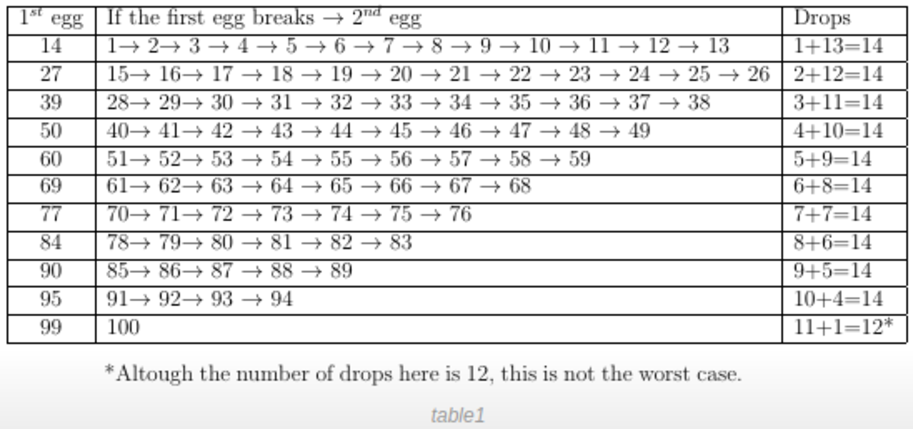
\includegraphics[width=0.8\textwidth]{Images/figBrilliantEggDropTab}
%\caption[]{}
%\label{figBrilliantEggDropTab}
\end{figure}

Using other strategies, like the binary search, fewer attempts would be
required in some cases (like in our first example), but it would require a
high number of attempts in the worst case (in our second example, where the
egg broke in the $50$th floor and $50$ drops were necessary in the worst
case).

Therefore, we can conclude that using another strategy you would need more
than $14$ attempts in the worst case.

\rrheader{$2$ Eggs, $k$ Floors\label{rrED2EggskFloors}}

Now let's try to find a solution for the case where you have $2$ eggs and a
building with $k$ floors.

A good way to start this problem is to ask ``Are we able to cover all the
floors with $x$ drops?''

Suppose that in the best strategy, the number of drops in the worst case is
$x$. Then, you should start at the $x$th floor, because if the egg breaks,
you will have to check floors $1,2,3,\ldots,x-2$ and $x-1$, so the total
number of drops will be $x$. If it doesn't break, you will have to check the
$(x+(x-1))$th floor. If the egg breaks, you will have to check the floors
$x+1$, $x+2$, $\ldots$, $(x+(x-1)-1)$. Hence, the number of drops will be
$(x+(x-1)-1)-(x+1)+1+2=x$.

If you're confused about the last equation, consider this: We test at $14$th
floor and it doesn't break, so next we test at $14+(14-1)=14+13=27$th floor,
if it breaks, we'll have to test from $14+1$, $14+2$, $\ldots,$
$14+(14-1)-1=14+12=26$. Hence, the number of drops will be
$(14+(14-1)-1)-(14+1)+1+2=14$..... actually, I still dunno where the two +1
comes from. I should just do $(14+(14-1)-1)-14 + 2=14$, makes more sense to
me.

Do you realize what we are doing? Based on the assumption that the number of
drops will always be $x$ in the worst case, we find the floors where we
should drop the egg. The crucial point here is understanding that we are not
trying to find the minimum number of drops knowing the best strategy;
actually, we are trying to find the best strategy supposing that the minimum
number of drops is $x$, and we have to determine if covering all the floors
using at most attempts is possible or not.

We can find an analytical solution to this problem:

\begin{mdframed}[style=mdfNOTE,
frametitle={Example}]

Suppose the minimum number of attempts in the worst case, while using the
best strategy, is $x$. In our attempt, we will drop the egg at the $x$th
floor, covering $x$ floors, then we will drop it at the $(x+(x-1))$th floor,
covering $x-1$ floors, and the third drop would be at the
$(x+(x-1)+(x-2))$th floor, covering $x-2$ floors. We can see that using this
strategy we would cover
\begin{equation*}
x+(x-1)+(x-2)+(x-3)+\cdots+2+1=\frac{x(x+1)}{2}
\end{equation*}
floors.

If we are able to cover $\frac{x(x+1)}{2}$ floors using this strategy and
the building has $k$ floors, we just have to find the minimum value of $x$
such that
\begin{equation*}
\frac{x(x+1)}{2}\geq k.
\end{equation*}
Hence,
\begin{equation*}
x^2+x-2k = 0 \implies x = \frac{-1\pm\sqrt{1+8k}}{2}.
\end{equation*}
But  must be an integer, implying
\begin{equation*}
x=\ceil*{\frac{-1\pm\sqrt{1+8k}}{2}}.
\end{equation*}
In our first example, $k=100$, so plugging it into the previous equation
gives $\ceil*{13.65}=14$.

\end{mdframed}

\rrheader{$N$ Eggs, $k$ Floors\label{rrEDNEggskFloors}}

Suppose you have $N$ eggs and you want to determine from which floors in a
$k$-floor building you can drop an egg such that is doesn't break. You are
to determine the minimum number of attempts you need in order find the
critical floor in the \textbf{worst case} while using the best strategy. Now
the problem is a bit more complicated because we must find a general
solution for any number of eggs and floors. There are three different
solutions:
\begin{itemize}%[noitemsep,topsep=0pt]
\item \textbf{The recursive solution:} \\
This solution is more straightforward and can be implemented with ease, but
it is also the slowest one. Using this solution on programming contests is
not advisable due to its bad performance.
\item \textbf{The dynamic programming solution:} \\
This solution is similar to the previous one, but it's faster and may be
used to solve the problem for medium or small values of $k$ and $N$.
\item \textbf{A solution that combines both binary search and recursion:} \\
This is the faster one, and once the strategy is understood, it is rather
easy to implement.
\end{itemize}

\rrheader{Recursive Solution\label{rrED2RecurSol}}

Imagine the following situation: you have $n$ eggs and $h$ consecutive
floors yet to be tested, and afterward you drop the egg at floor $i$ in this
sequence of $h$ consecutive floors:
\begin{itemize}%[noitemsep,topsep=0pt]
\item If the eggs breaks: \\
The problem reduces to $n-1$ eggs and $i-1$ remaining floors.
\item If it doesn't break: \\ The problem reduces to $n$ eggs and $h-i$
  remaining floors. This is an important point. \textbf{The floors we want
    to test aren't important; in fact, \emph{the number of remaining floors
      is what matters}.} For example, testing the floors between 1 and 20
  (both 1 and 20 included) would require the same number of drops to test
  the floors between 21 and 40, or between 81 and 100. In all three
  situations, we tested 20 floors.
\end{itemize}

Now we can define a function $W(n,h)$ that computes the minimum number of
drops required to find the critical floor in the worst case scenario,
\textbf{whilst using the best strategy}.

We can codify the above findings to find the following recursion for
determining $W(n,h)$:

\begin{mdframed}[style=mdfNOTE,
frametitle={Definition}]

\rrheader{Recursion for the egg dropping puzzle:}

\begin{equation*}
W[n,h]=1+\min\paren*{\max \paren*{W(n-1,i-1),W(n,h-i)}}.
\end{equation*}

\end{mdframed}
(Pay attention: $n$=current number of eggs, $N$=total number of eggs,
$h$=number of consecutive floors that still have to be tested, $k$=number of
floors in the building.)

The basis cases are as follows:
\begin{itemize}%[noitemsep,topsep=0pt]
\item Because we need $h$ drops if only $1$ egg remains, $W(1,h) = h$.
\item Because we need only one drop to test one floor, regardless of the
  number of eggs, $W(n,1) = 1$.
\item Because $0$ floors requires no drops, $W(n,0)=0$.
\end{itemize}

\begin{figure}
\centering
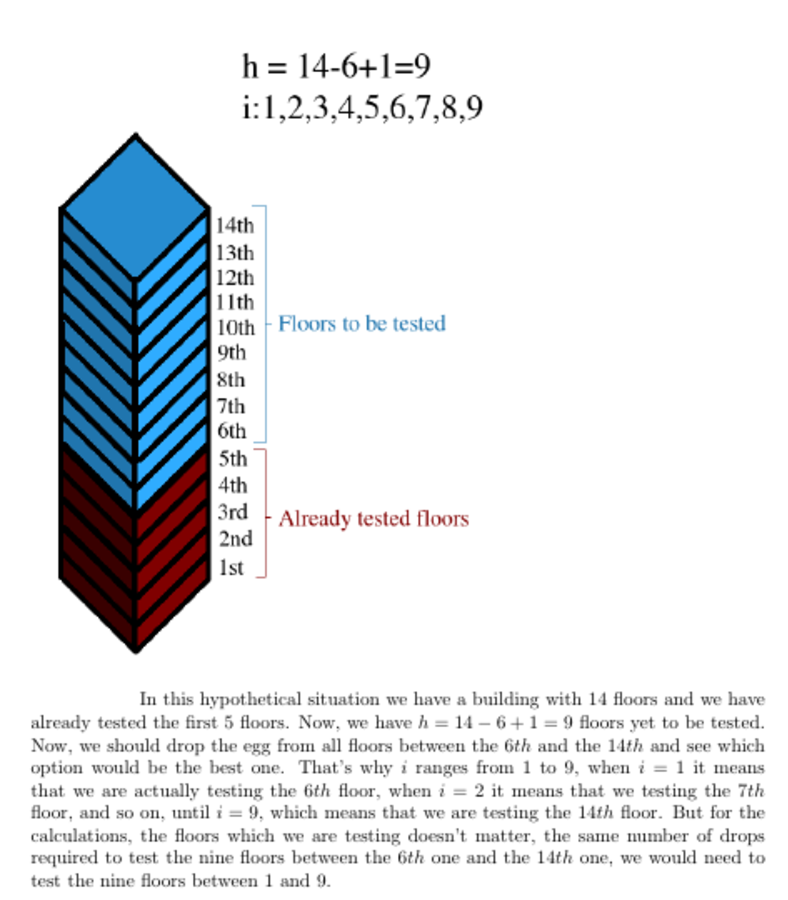
\includegraphics[width=0.9\textwidth]{Images/figBrilliantEggDropTower.ps}
%\caption[]{}
%\label{figBrilliantEggDropTower.ps}
\end{figure}

The pseudo-code for this algorithm is given by
\begin{lstlisting}[style=pseudostyle]
def drops(n,h):
  if(n == 1 or k == 0 or k == 1):
    return k
  end if

  minimum = infty

  for x = 1 to h:
    minimum = min(minimum, 
                  1 + max(drops(n - 1, x - 1), drops(n, h - x))
                  )
  end for

  return minimum
\end{lstlisting}
C++ code that uses the recursive solution:
\begin{lstlisting}[style=raycppnewsnippet]
#include <iostream>
#include <limits.h>

using namespace std;

//Compares 2 values and returns the bigger one
int max(int a,int b) {
  int ans=(a>b)?a:b;
  return ans;
}

//Compares 2 values and returns the smaller one
int min(int a,int b){
  int ans=(a<b)?a:b;
  return ans;
}

int egg(int n,int h){

  //Basis case
  if(n==1) return h;
  if(h==0) return 0;
  if(h==1) return 1;

  int minimum=INT_MAX;

  //Recursion to find egg(n,k). The loop iterates i: 1,2,3,...h
  for(int x=1;x<=h;x++) 
    minimum=min(minimum,
                (1+max(egg(n,h-x),
                       egg(n-1,x-1)
                      )
                 )
                );

    return minimum;
}

int main()
{
  int e;//Number of eggs
  int f;//Number of floors

  cout<<"Egg dropping puzzle\n\nNumber of eggs:";

  cin>>e;

  cout<<"\nNumber of floors:";

  cin>>f;

  cout<<"\nNumber of drops in the worst case:"<<egg(e,f);

  return 0;
}
\end{lstlisting}

\qasepline{}

Here's my attempt, code found in\\
\path{src/DynamicProgramming/rrrGFGDPSet11EggDrop.cpp}
\begin{lstlisting}[style=raycppnewsnippet]
// n - number of eggs
// h - number of floors to be tested
int eggDropRecur(int n, int h)
{
  // Base cases:
  // If there is one egg (n=1) and some floors (h>0), then we always need
  // to test every floor
  if(n==1 && h>0) return h;

  // If there are no floors to be tested (h=0), no drops are required.
  if(h==0) return 0;

  // If there is one floor to be tested, we need 1 drop.
  if(h==1) return 1;

  // Now, we test all floors from x=[1..h].
  // Each drop will give two subproblems:
  //   one for the lower half (if egg breaks)-> x-1 floors to test
  //   one for the upper half (if egg doesn't break)-> h-x floors to test
  // we take the max of the result of the two subproblems 
  // (to get the worst case answer)
  // However, we take the min over all droppings, since we do want the 
  // minimum dropping over the worst case.
  int minimum = std::numeric_limits<int>::max();
  for(int x = 1; x<=h; ++x)
  {
    minimum = std::min(minimum,
                       (1+std::max(eggDropRecur(n-1,x-1), // egg broke
                                   eggDropRecur(n  ,h-x)) // egg no break
                       )
                      );
  }
  return minimum;
}
\end{lstlisting}

\qasepline{}

\rrheader{DP Solution\label{rrEDDPSol}}

The previous solution is very slow, and the same function is called more
than once, which is not necessary. However, due to its overlapping
subproblems, and to its optimal substructure property (we can find the
solution to the problem using the subproblem's optimal solutions), we can
solve the problem via dynamic programming.

We can avoid recalculation of the same subproblems by memoizing the function
egg(n,h) with a two-dimensional array \ctt{numdrops[n][h]}. Then, we just
have to fill it up.

Here's the pseudocode:
\begin{lstlisting}[style=pseudostyle]
def solvepuzzle(N,k):
  for i = 1 to N
    numdrops(i,1) = 1
    numdrops(i,0) = 0
  end for

  for i=1 to k
    numdrops(1, i) = i
  end for

  for i = 2 to N
    for j = 2 to k 

      numdrops[i][j] = infty
      minimum = infty

      for x = 1 to j
        minimum = min(minimum, 
                      1 + max(numdrops(i-1,x-1),numdrops(i,j-x))
                     )
      end for

      numdrops[i][j] = minimum

    end for
  end for

  return numdrops(N,k)
\end{lstlisting}
C++ code:
\begin{lstlisting}[style=raycppnewsnippet]
#include <iostream>
#include <limits.h>

using namespace std;

//Compares 2 values and returns the bigger one
int max(int a,int b) {
  int ans=(a>b)?a:b;
  return ans;
}

//Compares 2 values and returns the smaller one
int min(int a,int b){
  int ans=(a<b)?a:b;
  return ans;
}

int solvepuzzle(int n,int k){

  int numdrops[n+1][k+1];
  int i,j,x;

  for(i=0;i<=k;i++) numdrops[0][i]=0;
  for(i=0;i<=k;i++) numdrops[1][i]=i;
  for(j=0;j<=n;j++) numdrops[j][0]=0;

  //This loop fills up the matrix
  for(i=2;i<=n;i++){
    for(j=1;j<=k;j++){

      //Defines the minimum as the highest possible value
      int minimum=INT_MAX;

      //Evaluates 1+min{max(numeggs[i][j-x],numeggs[i-1][x-1])), for x:1,2,3...j-1,j}
      for(x=1;x<=j;x++) minimum=min(minimum,(1+max(numdrops[i][j-x],numdrops[i-1][x-1])));


      //Defines the minimum value for numeggs[i][j]
      numdrops[i][j]=minimum;
    }

  }

  cout<<"\nArray:\n\n";

  //Prints numeggs
  for(i=0;i<=n;i++){
    for(j=0;j<=k;j++){
      cout<<numdrops[i][j]<<" ";
     }
     cout<<"\n";
  }

  cout<<"\nNumber of trials in the worst case using the best strategy:\n";

  return numdrops[n][k];
}

int main()
{
  int e;//Number of eggs
  int f;//Number of floors

  cout<<"Egg dropping puzzle\n\nNumber of eggs:";

  cin>>e;

  cout<<"\nNumber of floors:";

  cin>>f;

  cout<<solvepuzzle(e,f);

  return 0;
}
\end{lstlisting}

\qasepline{}

I will do bottom up. First, we need a table to store the results in a table
$dp[n+1][k+1]$, where $n=$number of eggs and $k=$number of floor in the
building. We need $+1$ since we're including $0$ eggs and floors. Thus,
$dp[n,k]$ represents the min. number of drop in the worst case for $n$ eggs
and $k$ floors.

First we fill in the base case: For $W(n,k)$, recall:
\begin{itemize}%[noitemsep,topsep=0pt]
\item One egg: $W(n=1,k)=k$.
\item One floor: $W(n,k=1)=1$.
\item Zero floor: $W(n,k=0)=0$.
\end{itemize}
\begin{tabular}{|c|c|c|c|c|c|}\hline
\diagbox{$n$}{$k$}&\textbf{0}&\textbf{1}&\textbf{2}&\textbf{3}&\textbf{4}\\\hline
\textbf{0}&0&1&&&\\\hline 
\textbf{1}&0&1&2&3&4\\\hline
\textbf{2}&0&1&&&\\\hline
\textbf{3}&0&1&&&\\\hline
\textbf{4}&0&1&&&\rrred{(X)}\\\hline
\end{tabular}\\
Now, the recursive call is:
\begin{lstlisting}[style=raycppnewsnippet]
for i=[2..n]
  for j=[2..k]
    for x = [1..j]
      eggDropRecur(i-1,x-1) // egg broke
      eggDropRecur(i  ,j-x) // egg no break
\end{lstlisting}
For now, we will assume that we work in row major order. This may change
depending on the dependencies, for example, if we have:
\begin{equation*}
dp[i,j] = [i,i-1]
\end{equation*}
then it'll make sense to work down the columns first, since each
\ctt{dp[i,j]} depends on the one above it. For 
\ctt{eggDropRecur(i-1,j-1)}, we're getting the solution for \ctt{[i,j]} from
the top left cell, so working in row major order works. What about
\ctt{eggDropRecur(i,j-x)}? Well, we're working on the same row as
\ctt{[i,j]}, but what is \ctt{j-x}? Let's work this out:
\begin{lstlisting}[style=raygeneric]
j=2, x=[1, 2]
j-x:    1  0

j=3, x=[1, 2, 3]
j-x:    2  1  0

j=4, x=[1, 2, 3, 4]
j-x:    3  2  1  0
\end{lstlisting}
So as you can see, each $j$ depends on only previous $j$'s (as opposed to
just the one previous $j$). Thus, it is actually okay to go in row major
order all the way! In fact, it is necessary, because to do (look at the
table \ctt{dp} whilst doing this, it makes more sense), let $i=2$ (the first
row we have to calculate) and move across the columns ($j=$):
\begin{itemize}[noitemsep,topsep=0pt]
\item $(2,2)$, we need the solutions from $(2,1)$ and $(2,0)$, which are
  given by the base case (see the table above).
\item $(2,3)$, we need the solutions from $(3,2)$, $(3,1)$ and $(3,0)$
\end{itemize}
Thus, we must go from left to right!  To do We can do this easily! Let's
code up the DP version!

Here's my attempt, code found in\\
\path{src/DynamicProgramming/rrrGFGDPSet11EggDrop.cpp}
\begin{lstlisting}[style=raycppnewsnippet]
// n - number of eggs
// k - number of floors in the building.
int eggDropDP(const int n, const int k)
{
  // table to store results
  // rows = num eggs
  // column = num floors to be tested.
  vector<vector<int>> dp(n+1,vector<int>(k+1,0));
//  print_2dvec(dp,"initial dp:\n","\n");

  // base cases:
  // 1) If there is one egg (n=1), the required number of drops is the same
  // as the number of floors to be tested W(n=1,k)=k, i.e.:
  //   0 1 2 3 4
  //   ---------
  // 0|
  // 1|0 1 2 3 4
  // 2|
  // 3|
  // 4|
  for(int j=0; j <= k; ++j)
  {
    dp[1][j]=j;
  }
//  print_2dvec(dp,"n=1 dp:\n","\n");

  // Base case 2) If there are no floors (k=0), num drops=0
  //              If there is one floor (k=1), num drops=1
  // So we have
  //   0 1 2 3 4
  //   ---------
  // 0|0 1
  // 1|0 1 2 3 4
  // 2|0 1
  // 3|0 1
  // 4|0 1
  for(int i=0; i<=n; ++i)
  {
    dp[i][0]=0;
    dp[i][1]=1;
  }
//  print_2dvec(dp,"k=0 or 1 dp:\n","\n");


	// Fill rest of the entries in table using optimal substructure
	// property
  for (int i = 2; i <= n; i++)
  {
    for (int j = 2; j <= k; j++)
    {
      dp[i][j] = INT_MAX;
			for (int x = 1; x <= j; x++)
			{
				int res = 1 + std::max(dp[i-1][x-1], dp[i][j-x]);
				if (res < dp[i][j])
					dp[i][j] = res;
			}
		}
	}

  // Now loop through the rows (num of eggs)
  for(int i=2; i <= n; ++i)
  {
    // Now loop through the number of floors.
    for(int j=2; j<= k; ++j)
    {
      // Now we drop the egg from each floor from x=[1..j]
      dp[i][j] = std::numeric_limits<int>::max();
      for(int x=1; x<=j; ++x)
      {
        dp[i][j] = std::min(dp[i][j],(1+std::max(dp[i-1][x-1],
                                                 dp[i][j-x])
                                     )
                           );
      }
    }
  }

//  print_2dvec(dp,"dp:\n","\n");
  return dp[n][k];
}
\end{lstlisting}

\rrheader{Working with Binomials\label{rrEDWorkingWithBinom}}

Before advancing to the next section we must see some useful mathematical
relations related to binomials.

We know that
\begin{equation*}
C^m_k=C(n,k)=\binom{n}{k}=\frac{n!}{(n-k)!k!}
\end{equation*}
We also know that the Pascal triangle is

%\begin{figure}
%\centering
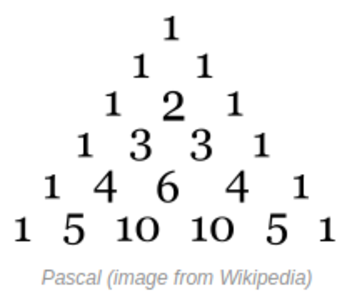
\includegraphics[width=0.2\textwidth]{Images/figBrilliantEggDropPascalsTri}
%\caption[]{}
%\label{figCXNX}
%\end{figure}

And we can easily find a recursion if we write the Pascal triangle in this
way:

%\begin{figure}
%\centering
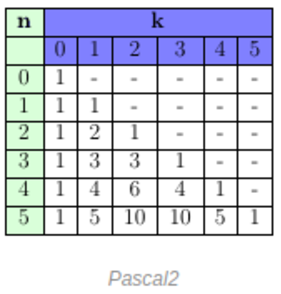
\includegraphics[width=0.3\textwidth]{Images/figBrilliantEggDropPascalsTri2}
%\caption[]{}
%\label{figCXNX}
%\end{figure}

By looking at the table or by a simple mathematical proof we get the
following recurrence:
\begin{equation*}
C(n,k)=C(n-1,k)+C(n-1,k-1),
\end{equation*}
And the basis cases are
\begin{equation*}
C(n,0)=\frac{n!}{(n-0)!0!}=1 \text{ and } C(n,n)=\frac{n!}{(n-n)!n!}=1
\end{equation*}

\rrheader{A Better Approach\label{rrEDABetterApproach}}

RRRTODO - I've given up on this for now. But it uses an identity in the code
at the end, which can be found in the wikipedia article:
\url{https://en.wikipedia.org/wiki/Dynamic\_programming#Egg\_dropping\_puzzle}


With this knowledge in hand, let's define a function $f(d,n)$ that
represents the \textbf{number of floors} we can cover using $n$ eggs and
with $d$ remaining drops.  If the egg breaks we will be able to cover
$f(d-1,n-1)$ floors, otherwise we'll be able to cover $f(d,n-1)$ floors.
Hence, the total number of floors we will be able to cover is
\begin{equation*}
f(d,n)=1+f(d-1,n-1)+f(d-1,n).
\end{equation*}

We must find a function $f(d,n)$ that's a solution for this recursion.
First, we will define an auxiliary function $g(d,n)$:
\begin{equation*}
g(d,n) = f(d,n+1)-f(d,n)
\end{equation*}

Plugging it into our first equation gives
This is precisely the same recursion that we saw in the previous section, and thus the function  can be written as
But we have a problem:  is 0 for every
, as well as , according to the relation between  and . However, a contradiction occurs when  because . But  should be  for every ! We can fix this problem by defining  as follows:
And the recursion is still valid (you can check it by yourself!).

Now, using a telescopic sum for , we can write it as
We know that , and therefore

And we also know that
Hence,
Finally,
Now that we have a nice formula for  how can we find the minimum number of drops?

It's simple! We know that  is the number of floors we can cover in the building with  floors using  eggs and no more than  drops in the worst cases. We simply have to find a value for  such that
Using our last formula,

This solution is very fast. We can do a linear search to find a value for , or we can binary search it for an even faster solution!

C++ code:

\begin{lstlisting}[style=raycppnewsnippet]
#include <iostream>
#include <math.h>

using namespace std;

//Evaluates C(n,k) and verifies if it's greater than or equal to k
long long binomial(int x,int n,int k){

    int i;
    long long int answer=0;
    double aux=1;

        //Calculates C(n,k) using the formula: C(n,k): sum_i_0^k {(n-i+1)/i}
    for(i=1;i<=n;i++){

            aux*=(float)x+1-i;
            aux/=(float)i;
            answer+=aux;

            if(answer>k) break;
    }

    return answer;
}

int main()
{
    int n; //Number of eggs
    int k; //Number of floors

    cout<<"Egg dropping puzzle: ( O(n log k)  solution )\n\n";

    cout<<"Number of floors:";
    cin>>k;

    cout<<"\nNumber of eggs:";
    cin>>n;

    //Binary search variables:
    //Mid: middle
    //Upper: upper limit
    //Inf: inferior limit

    int mid,upper,inf;

    upper=k;
    inf=0;
    mid=(upper+inf)/2;

    //Binary search
    while(upper-inf>1){

        //Finds the middle
        mid=inf+(upper-inf)/2;

        //Define new limits
        if(binomial(mid,n,k)<k) inf=mid;
        else upper=mid;

    }

    cout<<"\nNumber of drops in the worst case:"<<inf+1<<cout<<"\n";
}
\end{lstlisting}


\rrheader{See Also\label{rrEDSeeAlso}}

\begin{itemize}%[noitemsep,topsep=0pt]
\item Dynamic Programming \url{https://brilliant.org/wiki/problem-solving-dynamic-programming}
\end{itemize}

\rrheader{Complexity\label{rrEDComplexity}}

\begin{itemize}%[noitemsep,topsep=0pt]
\item $nk^2$
\item $n log k$ (from wikipedia)
\end{itemize}

\RayNotesEnd

\textbf{\rrgreen{Back to geeksforgeeks solution.}}


\rrheader{No need for GFG solution, the above is more than sufficient.}

In this post, we will discuss solution to a general problem with n eggs and
k floors. The solution is to try dropping an egg from every floor (from 1 to
k) and recursively calculate the minimum number of droppings needed in worst
case. The floor which gives the minimum value in worst case is going to be
part of the solution.

In the following solutions, we return the minimum number of trials in worst
case; these solutions can be easily modified to print floor numbers of every
trials also.

\rrheader{(1) Optimal Substructure:}

When we drop an egg from a floor x, there can be two cases (1) The egg
breaks (2) The egg doesn't break.
\begin{enumerate}[label=\textbf{\arabic*.}]
\item If the egg breaks after dropping from xth floor, then we only need to
  check for floors lower than x with remaining eggs; so the problem reduces
  to x-1 floors and n-1 eggs
\item If the egg doesn't break after dropping from the xth floor, then we
  only need to check for floors higher than x; so the problem reduces to k-x
  floors and n eggs.
\end{enumerate}

Since we need to minimize the number of trials in worst case, we take the
maximum of two cases. We consider the max of above two cases for every floor
and choose the floor which yields minimum number of trials.
\begin{lstlisting}[style=raygeneric]
  k ==> Number of floors
  n ==> Number of Eggs
  eggDrop(n, k) ==> Minimum number of trials needed to find the critical
                    floor in worst case.
  eggDrop(n, k) = 1 + min{max(eggDrop(n - 1, x - 1), eggDrop(n, k - x)): 
                 x in {1, 2, ..., k}}
\end{lstlisting}

\rrheader{(2) Overlapping Subproblems}

Following is recursive implementation that simply follows the recursive
structure mentioned above.
\begin{lstlisting}[style=raycppnewsnippet]
# include <stdio.h>
# include <limits.h>
 
// A utility function to get maximum of two integers
int max(int a, int b) { return (a > b)? a: b; }
 
/* Function to get minimum number of trials needed in worst
  case with n eggs and k floors */
int eggDrop(int n, int k)
{
    // If there are no floors, then no trials needed. OR if there is
    // one floor, one trial needed.
    if (k == 1 || k == 0)
        return k;
 
    // We need k trials for one egg and k floors
    if (n == 1)
        return k;
 
    int min = INT_MAX, x, res;
 
    // Consider all droppings from 1st floor to kth floor and
    // return the minimum of these values plus 1.
    for (x = 1; x <= k; x++)
    {
        res = max(eggDrop(n-1, x-1), eggDrop(n, k-x));
        if (res < min)
            min = res;
    }
 
    return min + 1;
}

/* Driver program to test to pront printDups*/
int main()
{
    int n = 2, k = 10;
    printf ("nMinimum number of trials in worst case with %d eggs and "
             "%d floors is %d n", n, k, eggDrop(n, k));
    return 0;
}
\end{lstlisting}
Output:
\begin{lstlisting}[style=rayio]
Minimum number of trials in worst case with 2 eggs and 10 floors is 4
\end{lstlisting}
It should be noted that the above function computes the same subproblems
again and again. See the following partial recursion tree, E(2, 2) is being
evaluated twice. There will many repeated subproblems when you draw the
complete recursion tree even for small values of n and k.
\begin{lstlisting}[style=raygeneric]
                         E(2,4)
                           |                      
          ------------------------------------- 
          |             |           |         |   
          |             |           |         |       
      x=1/          x=2/      x=3/     x=4/ 
        /             /         ....      ....
       /             /    
 E(1,0)  E(2,3)     E(1,1)  E(2,2)
          /  /...         /  
      x=1/                 .....
        /    
     E(1,0)  E(2,2)
            /   
            ......

Partial recursion tree for 2 eggs and 4 floors.
\end{lstlisting}
Since same suproblems are called again, this problem has Overlapping
Subprolems property. So Egg Dropping Puzzle has both properties (see this
and this) of a dynamic programming problem. Like other typical Dynamic
Programming(DP) problems, recomputations of same subproblems can be avoided
by constructing a temporary array eggFloor[][] in bottom up manner.

\rrheader{Dynamic Programming Solution}

Following are C++ and Python implementations for Egg Dropping problem using
Dynamic Programming.
\begin{lstlisting}[style=raycppnewsnippet]
# A Dynamic Programming based C++ Program for the Egg Dropping Puzzle
# include <stdio.h>
# include <limits.h>
 
// A utility function to get maximum of two integers
int max(int a, int b) { return (a > b)? a: b; }
 
/* Function to get minimum number of trials needed in worst
  case with n eggs and k floors */
int eggDrop(int n, int k)
{
    /* A 2D table where entery eggFloor[i][j] will represent minimum
       number of trials needed for i eggs and j floors. */
    int eggFloor[n+1][k+1];
    int res;
    int i, j, x;
 
    // We need one trial for one floor and0 trials for 0 floors
    for (i = 1; i <= n; i++)
    {
        eggFloor[i][1] = 1;
        eggFloor[i][0] = 0;
    }
 
    // We always need j trials for one egg and j floors.
    for (j = 1; j <= k; j++)
        eggFloor[1][j] = j;

    // Fill rest of the entries in table using optimal substructure
    // property
    for (i = 2; i <= n; i++)
    {
        for (j = 2; j <= k; j++)
        {
            eggFloor[i][j] = INT_MAX;
            for (x = 1; x <= j; x++)
            {
                res = 1 + max(eggFloor[i-1][x-1], eggFloor[i][j-x]);
                if (res < eggFloor[i][j])
                    eggFloor[i][j] = res;
            }
        }
    }
 
    // eggFloor[n][k] holds the result
    return eggFloor[n][k];
}
 
/* Driver program to test to pront printDups*/
int main()
{
    int n = 2, k = 36;
    printf ("nMinimum number of trials in worst case with %d eggs and "
             "%d floors is %d n", n, k, eggDrop(n, k));
    return 0;
}
\end{lstlisting}
Output:
\begin{lstlisting}[style=rayio]
Minimum number of trials in worst case with 2 eggs and 36 floors is 8
\end{lstlisting}
\rrhl{Time Complexity:} $\comBigOh{nk^2}$\\
\rrhl{Auxiliary Space:} $\comBigOh{nk}$

As an exercise, you may try modifying the above DP solution to print all
intermediate floors (The floors used for minimum trial solution).

2 Eggs and 100 Floor
Puzzle\footnote{\url{http://www.geeksforgeeks.org/puzzle-set-35-2-eggs-and-100-floors}}

%%%%%%%%%%%%%%%%%%%%%%%%%%%%%%%%%%%%%%%%%%%%%%%%%%%%%%%%%%%%%%%%%%%%%%%%%%%%
%%%%%%%%%%%%%%%%%%%%%%%%%%%%%%%%%%%%%%%%%%%%%%%%%%%%%%%%%%%%%%%%%%%%%%%%%%%%
%%%%%%%%%%%%%%%%%%%%%%%%%%%%%%%%%%%%%%%%%%%%%%%%%%%%%%%%%%%%%%%%%%%%%%%%%%%%

\section{Dynamic Programming | Set 12 (Longest Palindromic Subsequence)
  \label{secGFGDPSet12LongPalinSubseq}}

\url{http://www.geeksforgeeks.org/dynamic-programming-set-12-longest-palindromic-subsequence}

\textbf{Difficulty: 3.4}

Given a sequence, find the length of the longest palindromic subsequence in
it.
\begin{lstlisting}[style=raygeneric]
Input: GEEKSFORGEEKS
Output: 5

The longest palindromic subsequence we can get is of length 5.
There are more than one palindromic subsequences of length 5,
for example, EEKEE, EESEE, EEFEE, ...
\end{lstlisting}
As another example, if the given sequence is ``BBABCBCAB'', then the output
should be 7 as ``BABCBAB'' is the longest palindromic subseuqnce in it.
``BBBBB'' and ``BBCBB'' are also palindromic subsequences of the given
sequence, but not the longest ones.

\textbf{\rrgreen{Recommended: Please try your approach first, before moving
    on to the solution.}}

\RayNotesBegin

Okay, assume that we have a string $X$, of length $n$, so that $X[0..n-1]$.
Now we think about how we'll express the length of the longest palindromic
subsequence recursively. What are that states? We know that we have to work
from both ends of the string, so let the states be $(i,j)$, where $0\leq
i\leq j\leq n-1$,
denote the indices of the string. Suppose that $L(i,j)$ is the length of the
LPS of $X[i..j]$.
\begin{itemize}%[noitemsep,topsep=0pt]
\item If $X[i]==X[j]$, then these two chars are a part of the subsequence,
  thus we have a subproblem of $L(i+1,j-1)$. That is: 
  \begin{equation*}
  L(i,j)=L(i+1,j-1)+2.
  \end{equation*}
\item If $X[i]\neq X[j]$, then these two chars do not together form part of
  the palindrome, so we have two subproblems, each with either $X[i]$ or
  $X[j]$ taken off, and we need the max length of the two, i.e:
  \begin{equation*}
  L(i,j)=max(L(i+1,j),L(i,j-1)).
  \end{equation*}
\end{itemize}

Base cases: We either take two chars off or one char off. So the base case
lengths are 0, 1 or 2. Note that since the indices are inclusive, i.e.
$X[i..j]$ includes both $X[i]$ and $X[j]$, a char of size 1 would occur if
$X[i==j]$, and $j<i$ (which represents no char) is invalid. Also, note that
due to this, to get the number of elements indicated by $i$ and $j$, we need
to take the difference $j-i$ plus 1 (i.e. $j-i+1$), this is similar to the
number of matrices in chain matrix mult. I make this point since it is in
stark contrast to how iterators work, where \ctt{end()} is normally one past
the last element, so to get the number of elements in the range
\ctt{begin()} and \ctt{end()}, we simply do $end-begin$. Another way to look
at it is:
\begin{itemize}[noitemsep,topsep=0pt]
\item If the range is $[i,j]$, then the number of elements in the range is
  $(j-i+1)$.
\item If the range if $[i,j)$, then the number of elements in the range is
  $(j-i)$.
\end{itemize}
Now for the base cases:
\begin{itemize}[noitemsep,topsep=0pt]
\item $j<i$, no elements, return 0.
\item $i==j$, one char, each char is  palindrome of length 1, return 1.
\item $j-i+1==2$ and $X[i]==X[j]$, this is a palindrome of length 2, return
  2.
\item Otherwise, do the recursion as indicated above.
\end{itemize}
Now let's code this up! Code found in\\
\path{src/DynamicProgramming/rrrGFGDPSet12LPS.cpp}
\begin{lstlisting}[style=raycppnewsnippet]
int LPS(string& X, int i, int j)
{
  // We do the base cases from decreasing length, since, size 2 is more 
  // likely to happen before size 1 or size 0.
  
  if( ((j-i)==1) && X[i]==X[j]) // size 2
    return 2;
  if(j==i)
    return 1;
  if(j<i)
    return 0;

  // recursive case
  if(X[i]==X[j])
  {
    // plus two since we took two off.
    return LPS(X,i+1,j-1) + 2;
  }
  else
  {
    // No palindrome contributions found.
    return std::max(LPS(X,i+1,j),LPS(X,i,j-1));
  }
  return 0;
}
void runLPS(string& str)
{
  cout << "LPS: " << LPS(str,0,str.size())<<'\n';
}
\end{lstlisting}
Now let's do the DP version. Let's define a table $dp[n+1][n+1]$, where $n$
is the length of the string. We add 1 for length $0$ case. We will in the
base cases for $dp[j==i]=1$ and $dp[j<i]=0$\\
\begin{tabular}{|c|c|c|c|c|c|}\hline
\diagbox{$i$}{$j$}&0&1&2&3&4\\\hline
0&1&&&&\\\hline 
1&0&1&&&\rrred{(X)}\\\hline
2&0&0&1&&\\\hline
3&0&0&0&1&\\\hline
4&0&0&0&0&1\\\hline
\end{tabular}\\
Looking at the recursive definition, then we know that we work from shorter
lengths to longer lengths, until we get to $dp[1,n]$, which is the answer we
need. Now, we know we have to loop through all substrings of length 1, then
length 2, etc... To help us visualise this, we will put the lengths on a
table:\\
\begin{tabular}{|c|c|c|c|c|c|}\hline
\diagbox{$i$}{$j$}&0&1&2&3&4\\\hline
0&1&&&&\\\hline 
1&0&1&2&3&\rrred{(4)}\\\hline
2&0&0&1&2&3\\\hline
3&0&0&0&1&2\\\hline
4&0&0&0&0&1\\\hline
\end{tabular}\\
So clearly, we have to loop through the diagonals, then off diagonals. This
is exactly the same as in matrix chain multiplication (see
\pagecref{secGFGDPSet8MatChainMult}.
Another way to think about this is, we have to loop through the indices
$(i,j)$ for which $j-i+1=l$, for $l=1..n$. So, we know that $l=[1..n]$, what
about the range of $i$, since if we have $i$, we can use this to get $j$ by
$j=l+i-1$ (from $j-i+1=l$). By looking at the table above, we see that for
lengths $l=1$, $i=[1..4]$, for $l=2$, $i=[1..3]$. That is, the end of $i$,
which would normally end at $i=n$, gets less as we increase $l$. So we can
do $i=[1..n-l]$. But $n-l=4-l=3,2,1,0$ for $l=1,2,3,4$, we need it to go
from $4,3,2,1$. So we simply add one! $i=n-l+1$ for $l=[1..n]$. In
pseudocode we have the loops:
\begin{lstlisting}[style=pseudostyle,numbers=none]
for(int l = 1..n)
{
  for(int i = 1..(n-l+1))
  {
    j=l+i-1

    // base case for l=2, return 2 if X[i]==X[j]
    if(...)

    // X[i] and X[j] are the same
    if()
    else
     // ends are different
  }
}
\end{lstlisting}
Now let's code this up! Code found in\\
\path{src/DynamicProgramming/rrrGFGDPSet12LPS.cpp}
\begin{lstlisting}[style=raycppnewsnippet]
int LPSDP(string& X)
{
  int n = X.size();

  vector<vector<int>> dp(n+1,vector<int>(n+1,0));

  // First we fill in the base case for j==i
  for(int i=1; i<=n; ++i) dp[i][i]=1;

  // Loop through the lengths l=2..n (we have already done l=1)
  for(int l=2; l<=n; ++l)
  {
    // Loop through the i
    for(int i=1; i <= (n-l+1); ++i)
    {
      int j = l+i-1;

      // Base case of length 2
      if((l==2) && X[j]==X[i])
        dp[i][j]=2;
      else if(X[i]==X[j]) // ends are the same
      {
        dp[i][j] = 2+dp[i+1][j-1];
      }
      else // ends not the same
      {
        dp[i][j] = std::max(dp[i+1][j],dp[i][j-1]);
      }
    }
  }
  return dp[1][n];
}
void runLPSDP(string& str)
{
  cout << "LPSDP: " << LPSDP(str)<<'\n';
}
\end{lstlisting}
It works! Now let's continue with GFG solution.

\RayNotesEnd

\textbf{\rrgreen{Back to geeksforgeeks solution.}}

The na\"ive solution for this problem is to generate all subsequences of the
given sequence and find the longest palindromic subsequence. This solution
is exponential in term of time complexity $\comBigOh{2^n}$. Let us see how
this problem possesses both important properties of a Dynamic Programming
(DP) Problem and can efficiently solved using Dynamic Programming.

\rrheader{(1) Optimal Substructure:}

Let $X[0..n-1]$ be the input sequence of length $n$ and $L(0, n-1)$ be the
length of the longest palindromic subsequence of $X[0..n-1]$.
\begin{itemize}[noitemsep,topsep=0pt]
\item If last and first characters of $X$ are same, then
  $L(0,n-1)=L(1,n-2)+2$.
\item Else $L(0,n-1)=\max( L(1, n-1), L(0, n-2) )$.
\end{itemize}
Following is a general recursive solution with all cases handled.
\begin{lstlisting}[style=raygeneric]
// Every single character is a palindrome of length 1
L(i, i) = 1 for all indexes i in given sequence

// IF first and last characters are not same
If (X[i] != X[j])  L(i, j) =  max{L(i + 1, j),L(i, j - 1)} 

// If there are only 2 characters and both are same
Else if (j == i + 1) L(i, j) = 2  

// If there are more than two characters, and first and last 
// characters are same
Else L(i, j) =  L(i + 1, j - 1) + 2 
\end{lstlisting}

\rrheader{(2) Overlapping Subproblems}

Following is simple recursive implementation of the LPS problem. The
implementation simply follows the recursive structure mentioned above.
\begin{lstlisting}[style=raycppnewsnippet]
#include<stdio.h>
#include<string.h>
 
// A utility function to get max of two integers
int max (int x, int y) { return (x > y)? x : y; }
 
// Returns the length of the longest palindromic subsequence in seq
int lps(char *seq, int i, int j)
{
  // Base Case 1: If there is only 1 character
  if (i == j)
    return 1;
 
  // Base Case 2: If there are only 2 characters and both are same
  if (seq[i] == seq[j] && i + 1 == j)
    return 2;
 
  // If the first and last characters match
  if (seq[i] == seq[j])
     return lps (seq, i+1, j-1) + 2;
 
  // If the first and last characters do not match
  return max( lps(seq, i, j-1), lps(seq, i+1, j) );
}
 
/* Driver program to test above functions */
int main()
{
  char seq[] = "GEEKSFORGEEKS";
  int n = strlen(seq);
  printf ("The length of the LPS is %d", lps(seq, 0, n-1));
  getchar();
  return 0;
}
\end{lstlisting}
Output:
\begin{lstlisting}[style=rayio]
The length of the LPS is 5
\end{lstlisting}
Considering the above implementation, following is a partial recursion tree
for a sequence of length 6 with all different characters.
\begin{lstlisting}[style=raygeneric]
               L(0, 5)
             /        \ 
            /          \  
        L(1,5)          L(0,4)
       /    \            /    \
      /      \          /      \
  L(2,5)    L(1,4)  L(1,4)  L(0,3)
\end{lstlisting}
In the above partial recursion tree, $L(1,4)$ is being solved twice. If we
draw the complete recursion tree, then we can see that there are many
subproblems which are solved again and again. Since same suproblems are
called again, this problem has Overlapping Subprolems property. So LPS
problem has both properties (see this and this) of a dynamic programming
problem. Like other typical Dynamic Programming(DP) problems, recomputations
of same subproblems can be avoided by constructing a temporary array
\ctt{L[][]} in bottom up manner.

\rrheader{Dynamic Programming Solution}

\begin{lstlisting}[style=raycppnewsnippet]
# A Dynamic Programming based Python program for LPS problem
# Returns the length of the longest palindromic subsequence in seq
#include<stdio.h>
#include<string.h>
 
// A utility function to get max of two integers
int max (int x, int y) { return (x > y)? x : y; }
 
// Returns the length of the longest palindromic subsequence in seq
int lps(char *str)
{
  int n = strlen(str);
  int i, j, cl;
  int L[n][n];  // Create a table to store results of subproblems
 
 
  // Strings of length 1 are palindrome of lentgh 1
  for (i = 0; i < n; i++)
     L[i][i] = 1;
 
  // Build the table. Note that the lower diagonal values of table are
  // useless and not filled in the process. The values are filled in a
  // manner similar to Matrix Chain Multiplication DP solution (See
  // http://www.geeksforgeeks.org/archives/15553). cl is length of
  // substring
  for (cl=2; cl<=n; cl++)
  {
    for (i=0; i<n-cl+1; i++)
    {
      j = i+cl-1;
      if (str[i] == str[j] && cl == 2)
        L[i][j] = 2;
      else if (str[i] == str[j])
        L[i][j] = L[i+1][j-1] + 2;
      else
        L[i][j] = max(L[i][j-1], L[i+1][j]);
    }
  }
  return L[0][n-1];
}
 
/* Driver program to test above functions */
int main()
{
    char seq[] = "GEEKS FOR GEEKS";
    int n = strlen(seq);
    printf ("The lnegth of the LPS is %d", lps(seq));
    getchar();
    return 0;
}
\end{lstlisting}
Output:
\begin{lstlisting}[style=rayio]
The lnegth of the LPS is 7
\end{lstlisting}
Time Complexity of the above implementation is $\comBigOh{n^2}$ which is
much better than the worst case time complexity of Naive Recursive
implementation.

\begin{mdframed}[style=mdfNOTE,
frametitle={Using LCS}]
This problem is close to the Longest Common Subsequence (LCS) problem. In
fact, we can use LCS as a subroutine to solve this problem. Following is the
two step solution that uses LCS.
\begin{enumerate}[label=\textbf{\arabic*.}]
\item Reverse the given sequence and store the reverse in another array say
  \ctt{rev[0..n-1]}
\item LCS of the given sequence and \ctt{rev[]} will be the longest
  palindromic sequence.
\end{enumerate}
This solution is also a $\comBigOh{n^2}$ solution.
\end{mdframed}

%%%%%%%%%%%%%%%%%%%%%%%%%%%%%%%%%%%%%%%%%%%%%%%%%%%%%%%%%%%%%%%%%%%%%%%%%%%%
%%%%%%%%%%%%%%%%%%%%%%%%%%%%%%%%%%%%%%%%%%%%%%%%%%%%%%%%%%%%%%%%%%%%%%%%%%%%
%%%%%%%%%%%%%%%%%%%%%%%%%%%%%%%%%%%%%%%%%%%%%%%%%%%%%%%%%%%%%%%%%%%%%%%%%%%%

\section{Dynamic Programming | Set 13 (Cutting a Rod)
  \label{secGFGDPSet13CuttingARod}}

\url{http://www.geeksforgeeks.org/dynamic-programming-set-13-cutting-a-rod}

\textbf{Difficulty: 3.1}

Given a rod of length n inches and an array of prices that contains prices
of all pieces of size smaller than n. Determine the maximum value obtainable
by cutting up the rod and selling the pieces. For example, if length of the
rod is 8 and the values of different pieces are given as following, then the
maximum obtainable value is 22 (by cutting in two pieces of lengths 2 and 6)
\begin{lstlisting}[style=raygeneric]
length   | 1   2   3   4   5   6   7   8  
--------------------------------------------
price    | 1   5   8   9  10  17  17  20
\end{lstlisting}
And if the prices are as following, then the maximum obtainable value is 24
(by cutting in eight pieces of length 1)
\begin{lstlisting}[style=raygeneric]
length   | 1   2   3   4   5   6   7   8  
--------------------------------------------
price    | 3   5   8   9  10  17  17  20
\end{lstlisting}

\textbf{\rrgreen{Recommended: Please try your approach first, before moving
    on to the solution.}}

\RayNotesBegin



\RayNotesEnd

\textbf{\rrgreen{Back to geeksforgeeks solution.}}

A naive solution for this problem is to generate all configurations of
different pieces and find the highest priced configuration. This solution is
exponential in term of time complexity. Let us see how this problem
possesses both important properties of a Dynamic Programming (DP) Problem
and can efficiently solved using Dynamic Programming.

\rrheader{(1) Optimal Substructure:}

We can get the best price by making a cut at different positions and
comparing the values obtained after a cut. We can recursively call the same
function for a piece obtained after a cut.

Let cutRoad(n) be the required (best possible price) value for a rod of
lenght n. cutRod(n) can be written as following.

cutRod(n) = max(price[i] + cutRod(n-i-1)) for all i in {0, 1 .. n-1}

\rrheader{(2) Overlapping Subproblems}

Following is simple recursive implementation of the Rod Cutting problem. The
implementation simply follows the recursive structure mentioned above.

\begin{lstlisting}[style=raycppnewsnippet]
// A Naive recursive solution for Rod cutting problem
#include<stdio.h>
#include<limits.h>
 
// A utility function to get the maximum of two integers
int max(int a, int b) { return (a > b)? a : b;}
 
/* Returns the best obtainable price for a rod of length n and
   price[] as prices of different pieces */
int cutRod(int price[], int n)
{
  if (n <= 0)
    return 0;
  int max_val = INT_MIN;
 
  // Recursively cut the rod in different pieces and compare different 
  // configurations
  for (int i = 0; i<n; i++)
       max_val = max(max_val, price[i] + cutRod(price, n-i-1));
 
  return max_val;
}
 
/* Driver program to test above functions */
int main()
{
  int arr[] = {1, 5, 8, 9, 10, 17, 17, 20};
  int size = sizeof(arr)/sizeof(arr[0]);
  printf("Maximum Obtainable Value is %dn", cutRod(arr, size));
  getchar();
  return 0;
}
\end{lstlisting}
Output:
\begin{lstlisting}[style=rayio]
Maximum Obtainable Value is 22
\end{lstlisting}
Considering the above implementation, following is recursion tree for a Rod
of length 4.
\begin{lstlisting}[style=raygeneric]
cR() ---> cutRod() 

                             cR(4)
                  /        /           
                 /        /              
             cR(3)       cR(2)     cR(1)   cR(0)
            /  |         /         |
           /   |        /          |  
      cR(2) cR(1) cR(0) cR(1) cR(0) cR(0)
     /        |          |
    /         |          |   
  cR(1) cR(0) cR(0)      cR(0)
   /
 /
CR(0)
\end{lstlisting}
In the above partial recursion tree, cR(2) is being solved twice. We can see
that there are many subproblems which are solved again and again. Since same
suproblems are called again, this problem has Overlapping Subprolems
property. So the Rod Cutting problem has both properties (see this and this)
of a dynamic programming problem. Like other typical Dynamic Programming(DP)
problems, recomputations of same subproblems can be avoided by constructing
a temporary array val[] in bottom up manner.
\begin{lstlisting}[style=raycppnewsnippet]
// A Dynamic Programming solution for Rod cutting problem
#include<stdio.h>
#include<limits.h>
 
// A utility function to get the maximum of two integers
int max(int a, int b) { return (a > b)? a : b;}
 
/* Returns the best obtainable price for a rod of length n and
   price[] as prices of different pieces */
int cutRod(int price[], int n)
{
  int val[n+1];
  val[0] = 0;
  int i, j;
 
  // Build the table val[] in bottom up manner and return the last entry
  // from the table
  for (i = 1; i<=n; i++)
  {
    int max_val = INT_MIN;
    for (j = 0; j < i; j++)
      max_val = max(max_val, price[j] + val[i-j-1]);
    val[i] = max_val;
  }
 
  return val[n];
}
 
/* Driver program to test above functions */
int main()
{
  int arr[] = {1, 5, 8, 9, 10, 17, 17, 20};
  int size = sizeof(arr)/sizeof(arr[0]);
  printf("Maximum Obtainable Value is %dn", cutRod(arr, size));
  getchar();
  return 0;
}
\end{lstlisting}
Output:
\begin{lstlisting}[style=rayio]
Maximum Obtainable Value is 22
\end{lstlisting}
Time Complexity of the above implementation is $O(n^2)$ which is much better
than the worst case time complexity of Naive Recursive implementation.

Please write comments if you find anything incorrect, or you want to share
more information about the topic discussed above.

%%%%%%%%%%%%%%%%%%%%%%%%%%%%%%%%%%%%%%%%%%%%%%%%%%%%%%%%%%%%%%%%%%%%%%%%%%%%
%%%%%%%%%%%%%%%%%%%%%%%%%%%%%%%%%%%%%%%%%%%%%%%%%%%%%%%%%%%%%%%%%%%%%%%%%%%%
%%%%%%%%%%%%%%%%%%%%%%%%%%%%%%%%%%%%%%%%%%%%%%%%%%%%%%%%%%%%%%%%%%%%%%%%%%%%

\section{Dynamic Programming | Set 14 (Maximum Sum Increasing Subsequence)
  \label{secGFGDPSet14MaxSumIncreSunseq}}

\url{http://www.geeksforgeeks.org/dynamic-programming-set-14-maximum-sum-increasing-subsequence}

\textbf{Difficulty: 2.7}

\textbf{\rrgreen{Recommended: Please try your approach first, before moving
    on to the solution.}}

\RayNotesBegin



\RayNotesEnd

\textbf{\rrgreen{Back to geeksforgeeks solution.}}


%%%%%%%%%%%%%%%%%%%%%%%%%%%%%%%%%%%%%%%%%%%%%%%%%%%%%%%%%%%%%%%%%%%%%%%%%%%%
%%%%%%%%%%%%%%%%%%%%%%%%%%%%%%%%%%%%%%%%%%%%%%%%%%%%%%%%%%%%%%%%%%%%%%%%%%%%
%%%%%%%%%%%%%%%%%%%%%%%%%%%%%%%%%%%%%%%%%%%%%%%%%%%%%%%%%%%%%%%%%%%%%%%%%%%%

\section{Dynamic Programming | Set 15 (Longest Bitonic Subsequence)
  \label{secGFGDPSet15LongstBitonicSubseq}}

\url{http://www.geeksforgeeks.org/dynamic-programming-set-15-longest-bitonic-subsequence}

\textbf{Difficulty: 3.2}

\textbf{\rrgreen{Recommended: Please try your approach first, before moving
    on to the solution.}}

\RayNotesBegin



\RayNotesEnd

\textbf{\rrgreen{Back to geeksforgeeks solution.}}


%%%%%%%%%%%%%%%%%%%%%%%%%%%%%%%%%%%%%%%%%%%%%%%%%%%%%%%%%%%%%%%%%%%%%%%%%%%%
%%%%%%%%%%%%%%%%%%%%%%%%%%%%%%%%%%%%%%%%%%%%%%%%%%%%%%%%%%%%%%%%%%%%%%%%%%%%
%%%%%%%%%%%%%%%%%%%%%%%%%%%%%%%%%%%%%%%%%%%%%%%%%%%%%%%%%%%%%%%%%%%%%%%%%%%%

\section{Dynamic Programming | Set 16 (Floyd Warshall Algorithm)
  \label{secGFGDPSet16FloydWarshallAlgo}}

\url{http://www.geeksforgeeks.org/dynamic-programming-set-16-floyd-warshall-algorithm}

\textbf{Difficulty: 2.7}


\textbf{\rrgreen{Recommended: Please try your approach first, before moving
    on to the solution.}}

\RayNotesBegin



\RayNotesEnd

\textbf{\rrgreen{Back to geeksforgeeks solution.}}


%%%%%%%%%%%%%%%%%%%%%%%%%%%%%%%%%%%%%%%%%%%%%%%%%%%%%%%%%%%%%%%%%%%%%%%%%%%%
%%%%%%%%%%%%%%%%%%%%%%%%%%%%%%%%%%%%%%%%%%%%%%%%%%%%%%%%%%%%%%%%%%%%%%%%%%%%
%%%%%%%%%%%%%%%%%%%%%%%%%%%%%%%%%%%%%%%%%%%%%%%%%%%%%%%%%%%%%%%%%%%%%%%%%%%%

\section{Dynamic Programming | Set 17 (Palindrome Partitioning)
  \label{secGFGDPSet17PalinPartitioning}}

\url{http://www.geeksforgeeks.org/dynamic-programming-set-17-palindrome-partitioning}

\textbf{Difficulty: 4.4}

\textbf{\rrgreen{Recommended: Please try your approach first, before moving
    on to the solution.}}

\RayNotesBegin



\RayNotesEnd

\textbf{\rrgreen{Back to geeksforgeeks solution.}}


%%%%%%%%%%%%%%%%%%%%%%%%%%%%%%%%%%%%%%%%%%%%%%%%%%%%%%%%%%%%%%%%%%%%%%%%%%%%
%%%%%%%%%%%%%%%%%%%%%%%%%%%%%%%%%%%%%%%%%%%%%%%%%%%%%%%%%%%%%%%%%%%%%%%%%%%%
%%%%%%%%%%%%%%%%%%%%%%%%%%%%%%%%%%%%%%%%%%%%%%%%%%%%%%%%%%%%%%%%%%%%%%%%%%%%

\section{Dynamic Programming | Set 18 (Partition problem)
  \label{secGFGDPSet18PartitionProb}}

\url{http://www.geeksforgeeks.org/dynamic-programming-set-18-partition-problem}

\textbf{Difficulty: 3.5}


\textbf{\rrgreen{Recommended: Please try your approach first, before moving
    on to the solution.}}

\RayNotesBegin



\RayNotesEnd

\textbf{\rrgreen{Back to geeksforgeeks solution.}}


%%%%%%%%%%%%%%%%%%%%%%%%%%%%%%%%%%%%%%%%%%%%%%%%%%%%%%%%%%%%%%%%%%%%%%%%%%%%
%%%%%%%%%%%%%%%%%%%%%%%%%%%%%%%%%%%%%%%%%%%%%%%%%%%%%%%%%%%%%%%%%%%%%%%%%%%%
%%%%%%%%%%%%%%%%%%%%%%%%%%%%%%%%%%%%%%%%%%%%%%%%%%%%%%%%%%%%%%%%%%%%%%%%%%%%

\section{Dynamic Programming | Set 19 (Word Wrap Problem)
  \label{secGFGDPSet19WordWrapProb}}

\url{http://www.geeksforgeeks.org/dynamic-programming-set-18-word-wrap}

\textbf{Difficulty: 4.4}

\textbf{\rrgreen{Recommended: Please try your approach first, before moving
    on to the solution.}}

\RayNotesBegin



\RayNotesEnd

\textbf{\rrgreen{Back to geeksforgeeks solution.}}


%%%%%%%%%%%%%%%%%%%%%%%%%%%%%%%%%%%%%%%%%%%%%%%%%%%%%%%%%%%%%%%%%%%%%%%%%%%%
%%%%%%%%%%%%%%%%%%%%%%%%%%%%%%%%%%%%%%%%%%%%%%%%%%%%%%%%%%%%%%%%%%%%%%%%%%%%
%%%%%%%%%%%%%%%%%%%%%%%%%%%%%%%%%%%%%%%%%%%%%%%%%%%%%%%%%%%%%%%%%%%%%%%%%%%%

\section{Dynamic Programming | Set 20 (Maximum Length Chain of Pairs)
  \label{secGFGDPSet20MaxLenChainPairs}}

\url{http://www.geeksforgeeks.org/dynamic-programming-set-20-maximum-length-chain-of-pairs}

\textbf{Difficulty: 2.5}

\textbf{\rrgreen{Recommended: Please try your approach first, before moving
    on to the solution.}}

\RayNotesBegin



\RayNotesEnd

\textbf{\rrgreen{Back to geeksforgeeks solution.}}



%%%%%%%%%%%%%%%%%%%%%%%%%%%%%%%%%%%%%%%%%%%%%%%%%%%%%%%%%%%%%%%%%%%%%%%%%%%%
%%%%%%%%%%%%%%%%%%%%%%%%%%%%%%%%%%%%%%%%%%%%%%%%%%%%%%%%%%%%%%%%%%%%%%%%%%%%
%%%%%%%%%%%%%%%%%%%%%%%%%%%%%%%%%%%%%%%%%%%%%%%%%%%%%%%%%%%%%%%%%%%%%%%%%%%%

\section{Dynamic Programming | Set 21 (Variations of LIS)
  \label{secGFGDPSet21VariationsOfLIS}}

\url{http://www.geeksforgeeks.org/dynamic-programming-set-14-variations-of-lis}

\textbf{Difficulty: 3.5}

\textbf{\rrgreen{Recommended: Please try your approach first, before moving
    on to the solution.}}

\RayNotesBegin



\RayNotesEnd

\textbf{\rrgreen{Back to geeksforgeeks solution.}}


%%%%%%%%%%%%%%%%%%%%%%%%%%%%%%%%%%%%%%%%%%%%%%%%%%%%%%%%%%%%%%%%%%%%%%%%%%%%
%%%%%%%%%%%%%%%%%%%%%%%%%%%%%%%%%%%%%%%%%%%%%%%%%%%%%%%%%%%%%%%%%%%%%%%%%%%%
%%%%%%%%%%%%%%%%%%%%%%%%%%%%%%%%%%%%%%%%%%%%%%%%%%%%%%%%%%%%%%%%%%%%%%%%%%%%

\section{Dynamic Programming | Set 22 (Box Stacking Problem)
  \label{secGFGDPSet22BoxStackingProb}}

\url{http://www.geeksforgeeks.org/dynamic-programming-set-21-box-stacking-problem}

\textbf{Difficulty: 3.8}

\textbf{\rrgreen{Recommended: Please try your approach first, before moving
    on to the solution.}}

\RayNotesBegin



\RayNotesEnd

\textbf{\rrgreen{Back to geeksforgeeks solution.}}


%%%%%%%%%%%%%%%%%%%%%%%%%%%%%%%%%%%%%%%%%%%%%%%%%%%%%%%%%%%%%%%%%%%%%%%%%%%%
%%%%%%%%%%%%%%%%%%%%%%%%%%%%%%%%%%%%%%%%%%%%%%%%%%%%%%%%%%%%%%%%%%%%%%%%%%%%
%%%%%%%%%%%%%%%%%%%%%%%%%%%%%%%%%%%%%%%%%%%%%%%%%%%%%%%%%%%%%%%%%%%%%%%%%%%%

\section{Dynamic Programming | Set 23 (Bellman-Ford Algorithm)
  \label{secGFGDPSet23BellmanFordAlgo}}

\url{http://www.geeksforgeeks.org/dynamic-programming-set-23-bellman-ford-algorithm}

\textbf{Difficulty: 3.3}

\textbf{\rrgreen{Recommended: Please try your approach first, before moving
    on to the solution.}}

\RayNotesBegin



\RayNotesEnd

\textbf{\rrgreen{Back to geeksforgeeks solution.}}



%%%%%%%%%%%%%%%%%%%%%%%%%%%%%%%%%%%%%%%%%%%%%%%%%%%%%%%%%%%%%%%%%%%%%%%%%%%%
%%%%%%%%%%%%%%%%%%%%%%%%%%%%%%%%%%%%%%%%%%%%%%%%%%%%%%%%%%%%%%%%%%%%%%%%%%%%
%%%%%%%%%%%%%%%%%%%%%%%%%%%%%%%%%%%%%%%%%%%%%%%%%%%%%%%%%%%%%%%%%%%%%%%%%%%%

\section{Dynamic Programming | Set 24 (Optimal Binary Search Tree)
  \label{secGFGDPSet24OptimalBST}}

\url{http://www.geeksforgeeks.org/dynamic-programming-set-24-optimal-binary-search-tree}

\textbf{Difficulty: 4}

\textbf{\rrgreen{Recommended: Please try your approach first, before moving
    on to the solution.}}

\RayNotesBegin



\RayNotesEnd

\textbf{\rrgreen{Back to geeksforgeeks solution.}}


%%%%%%%%%%%%%%%%%%%%%%%%%%%%%%%%%%%%%%%%%%%%%%%%%%%%%%%%%%%%%%%%%%%%%%%%%%%%
%%%%%%%%%%%%%%%%%%%%%%%%%%%%%%%%%%%%%%%%%%%%%%%%%%%%%%%%%%%%%%%%%%%%%%%%%%%%
%%%%%%%%%%%%%%%%%%%%%%%%%%%%%%%%%%%%%%%%%%%%%%%%%%%%%%%%%%%%%%%%%%%%%%%%%%%%

\section{Dynamic Programming | Set 25 (Subset Sum Problem)
  \label{secGFGDPSet25SubsetSumProb}}

\url{http://www.geeksforgeeks.org/dynamic-programming-subset-sum-problem}

\textbf{Difficulty: 3.4}



\textbf{\rrgreen{Recommended: Please try your approach first, before moving
    on to the solution.}}

\RayNotesBegin



\RayNotesEnd

\textbf{\rrgreen{Back to geeksforgeeks solution.}}


%%%%%%%%%%%%%%%%%%%%%%%%%%%%%%%%%%%%%%%%%%%%%%%%%%%%%%%%%%%%%%%%%%%%%%%%%%%%
%%%%%%%%%%%%%%%%%%%%%%%%%%%%%%%%%%%%%%%%%%%%%%%%%%%%%%%%%%%%%%%%%%%%%%%%%%%%
%%%%%%%%%%%%%%%%%%%%%%%%%%%%%%%%%%%%%%%%%%%%%%%%%%%%%%%%%%%%%%%%%%%%%%%%%%%%

\section{Dynamic Programming | Set 26 (Largest Independent Set Problem)
  \label{secGFGDPSet26LargestIndepSetProb}}

\url{http://www.geeksforgeeks.org/largest-independent-set-problem}

\textbf{Difficulty: 3.4}


\textbf{\rrgreen{Recommended: Please try your approach first, before moving
    on to the solution.}}

\RayNotesBegin



\RayNotesEnd

\textbf{\rrgreen{Back to geeksforgeeks solution.}}


%%%%%%%%%%%%%%%%%%%%%%%%%%%%%%%%%%%%%%%%%%%%%%%%%%%%%%%%%%%%%%%%%%%%%%%%%%%%
%%%%%%%%%%%%%%%%%%%%%%%%%%%%%%%%%%%%%%%%%%%%%%%%%%%%%%%%%%%%%%%%%%%%%%%%%%%%
%%%%%%%%%%%%%%%%%%%%%%%%%%%%%%%%%%%%%%%%%%%%%%%%%%%%%%%%%%%%%%%%%%%%%%%%%%%%

\section{Dynamic Programming | Set 27 (Maximum sum rectangle in a 2D matrix)
  \label{secGFGDPSet27MaxSumRec2DMat}}

\url{http://www.geeksforgeeks.org/dynamic-programming-set-27-max-sum-rectangle-in-a-2d-matrix}

\textbf{Difficulty: 4.4}


\textbf{\rrgreen{Recommended: Please try your approach first, before moving
    on to the solution.}}

\RayNotesBegin



\RayNotesEnd

\textbf{\rrgreen{Back to geeksforgeeks solution.}}


%%%%%%%%%%%%%%%%%%%%%%%%%%%%%%%%%%%%%%%%%%%%%%%%%%%%%%%%%%%%%%%%%%%%%%%%%%%%
%%%%%%%%%%%%%%%%%%%%%%%%%%%%%%%%%%%%%%%%%%%%%%%%%%%%%%%%%%%%%%%%%%%%%%%%%%%%
%%%%%%%%%%%%%%%%%%%%%%%%%%%%%%%%%%%%%%%%%%%%%%%%%%%%%%%%%%%%%%%%%%%%%%%%%%%%

\section{Dynamic Programming | Set 28 (Minimum insertions to form a palindrome)
  \label{secGFGDPSet28MinmInsertnFormPalin}}

\url{http://www.geeksforgeeks.org/dynamic-programming-set-28-minimum-insertions-to-form-a-palindrome}

\textbf{Difficulty: 3.7}


\textbf{\rrgreen{Recommended: Please try your approach first, before moving
    on to the solution.}}

\RayNotesBegin



\RayNotesEnd

\textbf{\rrgreen{Back to geeksforgeeks solution.}}


%%%%%%%%%%%%%%%%%%%%%%%%%%%%%%%%%%%%%%%%%%%%%%%%%%%%%%%%%%%%%%%%%%%%%%%%%%%%
%%%%%%%%%%%%%%%%%%%%%%%%%%%%%%%%%%%%%%%%%%%%%%%%%%%%%%%%%%%%%%%%%%%%%%%%%%%%
%%%%%%%%%%%%%%%%%%%%%%%%%%%%%%%%%%%%%%%%%%%%%%%%%%%%%%%%%%%%%%%%%%%%%%%%%%%%

\section{Dynamic Programming | Set 29 (Longest Common Substring)
  \label{secGFGDPSet29LongstCommSubstr}}

\url{http://www.geeksforgeeks.org/longest-common-substring}

\textbf{Difficulty: 2.8}


\textbf{\rrgreen{Recommended: Please try your approach first, before moving
    on to the solution.}}

\RayNotesBegin



\RayNotesEnd

\textbf{\rrgreen{Back to geeksforgeeks solution.}}


%%%%%%%%%%%%%%%%%%%%%%%%%%%%%%%%%%%%%%%%%%%%%%%%%%%%%%%%%%%%%%%%%%%%%%%%%%%%
%%%%%%%%%%%%%%%%%%%%%%%%%%%%%%%%%%%%%%%%%%%%%%%%%%%%%%%%%%%%%%%%%%%%%%%%%%%%
%%%%%%%%%%%%%%%%%%%%%%%%%%%%%%%%%%%%%%%%%%%%%%%%%%%%%%%%%%%%%%%%%%%%%%%%%%%%

\section{Dynamic Programming | Set 30 (Dice Throw)
  \label{secGFGDPSet30DiceThrow}}

\url{http://www.geeksforgeeks.org/dice-throw-problem}

\textbf{Difficulty: 3.6}

\textbf{\rrgreen{Recommended: Please try your approach first, before moving
    on to the solution.}}

\RayNotesBegin



\RayNotesEnd

\textbf{\rrgreen{Back to geeksforgeeks solution.}}



%%%%%%%%%%%%%%%%%%%%%%%%%%%%%%%%%%%%%%%%%%%%%%%%%%%%%%%%%%%%%%%%%%%%%%%%%%%%
%%%%%%%%%%%%%%%%%%%%%%%%%%%%%%%%%%%%%%%%%%%%%%%%%%%%%%%%%%%%%%%%%%%%%%%%%%%%
%%%%%%%%%%%%%%%%%%%%%%%%%%%%%%%%%%%%%%%%%%%%%%%%%%%%%%%%%%%%%%%%%%%%%%%%%%%%

\section{Dynamic Programming | Set 31 (Optimal Strategy for a Game)
  \label{secGFGDPSet31OptStratForAGame}}

\url{http://www.geeksforgeeks.org/dynamic-programming-set-31-optimal-strategy-for-a-game}

\textbf{Difficulty: 4.1}


\textbf{\rrgreen{Recommended: Please try your approach first, before moving
    on to the solution.}}

\RayNotesBegin



\RayNotesEnd

\textbf{\rrgreen{Back to geeksforgeeks solution.}}

%%%%%%%%%%%%%%%%%%%%%%%%%%%%%%%%%%%%%%%%%%%%%%%%%%%%%%%%%%%%%%%%%%%%%%%%%%%%
%%%%%%%%%%%%%%%%%%%%%%%%%%%%%%%%%%%%%%%%%%%%%%%%%%%%%%%%%%%%%%%%%%%%%%%%%%%%
%%%%%%%%%%%%%%%%%%%%%%%%%%%%%%%%%%%%%%%%%%%%%%%%%%%%%%%%%%%%%%%%%%%%%%%%%%%%

\section{Dynamic Programming | Set 32 (Word Break Problem)
  \label{secGFGDPSet32WordBreakProb}}

\url{http://www.geeksforgeeks.org/dynamic-programming-set-32-word-break-problem}

\textbf{Difficulty: 3.8}



\textbf{\rrgreen{Recommended: Please try your approach first, before moving
    on to the solution.}}

\RayNotesBegin



\RayNotesEnd

\textbf{\rrgreen{Back to geeksforgeeks solution.}}

%%%%%%%%%%%%%%%%%%%%%%%%%%%%%%%%%%%%%%%%%%%%%%%%%%%%%%%%%%%%%%%%%%%%%%%%%%%%
%%%%%%%%%%%%%%%%%%%%%%%%%%%%%%%%%%%%%%%%%%%%%%%%%%%%%%%%%%%%%%%%%%%%%%%%%%%%
%%%%%%%%%%%%%%%%%%%%%%%%%%%%%%%%%%%%%%%%%%%%%%%%%%%%%%%%%%%%%%%%%%%%%%%%%%%%

\section{Dynamic Programming | Set 33 (Find if a string is interleaved of two other strings)
  \label{secGFGDPSet33FindIfStringIsInterleavedOfTwoOthers}}

\url{http://www.geeksforgeeks.org/check-whether-a-given-string-is-an-interleaving-of-two-other-given-strings-set-2}

\textbf{Difficulty: 4.3}


\textbf{\rrgreen{Recommended: Please try your approach first, before moving
    on to the solution.}}

\RayNotesBegin



\RayNotesEnd

\textbf{\rrgreen{Back to geeksforgeeks solution.}}

%%%%%%%%%%%%%%%%%%%%%%%%%%%%%%%%%%%%%%%%%%%%%%%%%%%%%%%%%%%%%%%%%%%%%%%%%%%%
%%%%%%%%%%%%%%%%%%%%%%%%%%%%%%%%%%%%%%%%%%%%%%%%%%%%%%%%%%%%%%%%%%%%%%%%%%%%
%%%%%%%%%%%%%%%%%%%%%%%%%%%%%%%%%%%%%%%%%%%%%%%%%%%%%%%%%%%%%%%%%%%%%%%%%%%%

\section{Dynamic Programming | Set 34 (Assembly Line Scheduling)
  \label{secGFGDPSet34AssemLineSchedul}}

\url{http://www.geeksforgeeks.org/dynamic-programming-set-34-assembly-line-scheduling}

\textbf{Difficulty: 2.7}


\textbf{\rrgreen{Recommended: Please try your approach first, before moving
    on to the solution.}}

\RayNotesBegin



\RayNotesEnd

\textbf{\rrgreen{Back to geeksforgeeks solution.}}

%%%%%%%%%%%%%%%%%%%%%%%%%%%%%%%%%%%%%%%%%%%%%%%%%%%%%%%%%%%%%%%%%%%%%%%%%%%%
%%%%%%%%%%%%%%%%%%%%%%%%%%%%%%%%%%%%%%%%%%%%%%%%%%%%%%%%%%%%%%%%%%%%%%%%%%%%
%%%%%%%%%%%%%%%%%%%%%%%%%%%%%%%%%%%%%%%%%%%%%%%%%%%%%%%%%%%%%%%%%%%%%%%%%%%%

\section{Dynamic Programming | Set 35 (Longest Arithmetic Progression)
  \label{secGFGDPSet35LongstArithProg}}

\url{http://www.geeksforgeeks.org/length-of-the-longest-arithmatic-progression-in-a-sorted-array}

\textbf{Difficulty: 4.6}


\textbf{\rrgreen{Recommended: Please try your approach first, before moving
    on to the solution.}}

\RayNotesBegin



\RayNotesEnd

\textbf{\rrgreen{Back to geeksforgeeks solution.}}

%%%%%%%%%%%%%%%%%%%%%%%%%%%%%%%%%%%%%%%%%%%%%%%%%%%%%%%%%%%%%%%%%%%%%%%%%%%%
%%%%%%%%%%%%%%%%%%%%%%%%%%%%%%%%%%%%%%%%%%%%%%%%%%%%%%%%%%%%%%%%%%%%%%%%%%%%
%%%%%%%%%%%%%%%%%%%%%%%%%%%%%%%%%%%%%%%%%%%%%%%%%%%%%%%%%%%%%%%%%%%%%%%%%%%%

\section{Dynamic Programming | Set 36 (Maximum Product Cutting)
  \label{secGFGDPSet36MaxProdCut}}

\url{http://www.geeksforgeeks.org/dynamic-programming-set-36-cut-a-rope-to-maximize-product}

\textbf{Difficulty: 3}

\textbf{\rrgreen{Recommended: Please try your approach first, before moving
    on to the solution.}}

\RayNotesBegin



\RayNotesEnd

\textbf{\rrgreen{Back to geeksforgeeks solution.}}


%%%%%%%%%%%%%%%%%%%%%%%%%%%%%%%%%%%%%%%%%%%%%%%%%%%%%%%%%%%%%%%%%%%%%%%%%%%%
%%%%%%%%%%%%%%%%%%%%%%%%%%%%%%%%%%%%%%%%%%%%%%%%%%%%%%%%%%%%%%%%%%%%%%%%%%%%
%%%%%%%%%%%%%%%%%%%%%%%%%%%%%%%%%%%%%%%%%%%%%%%%%%%%%%%%%%%%%%%%%%%%%%%%%%%%

\section{Dynamic Programming | Set 37 (Boolean Parenthesization Problem)
  \label{secGFGDPSet37BoolParenProb}}

\url{http://www.geeksforgeeks.org/dynamic-programming-set-37-boolean-parenthesization-problem}

\textbf{Difficulty: 4.5}


\textbf{\rrgreen{Recommended: Please try your approach first, before moving
    on to the solution.}}

\RayNotesBegin



\RayNotesEnd

\textbf{\rrgreen{Back to geeksforgeeks solution.}}







From top 20 DP:

http://www.geeksforgeeks.org/shortest-common-supersequence/

http://www.geeksforgeeks.org/count-number-of-ways-to-cover-a-distance/

http://www.geeksforgeeks.org/find-the-longest-path-in-a-matrix-with-given-constraints/



%%%%%%%%%%%%%%%%%%%%%%%%%%%%%%%%%%%%%%%%%%%%%%%%%%%%%%%%%%%%%%%%%%%%%%%%%%%%
%%%%%%%%%%%%%%%%%%%%%%%%%%%%%%%%%%%%%%%%%%%%%%%%%%%%%%%%%%%%%%%%%%%%%%%%%%%%
%%%%%%%%%%%%%%%%%%%%%%%%%%%%%%%%%%%%%%%%%%%%%%%%%%%%%%%%%%%%%%%%%%%%%%%%%%%%


http://www.geeksforgeeks.org/travelling-salesman-problem-set-1/

http://www.geeksforgeeks.org/travelling-salesman-problem-set-2-approximate-using-mst/


%%%%%%%%%%%%%%%%%%%%%%%%%%%%%%%%%%%%%%%%%%%%%%%%%%%%%%%%%%%%%%%%%%%%%%%%%%%%
%%%%%%%%%%%%%%%%%%%%%%%%%%%%%%%%%%%%%%%%%%%%%%%%%%%%%%%%%%%%%%%%%%%%%%%%%%%%
%%%%%%%%%%%%%%%%%%%%%%%%%%%%%%%%%%%%%%%%%%%%%%%%%%%%%%%%%%%%%%%%%%%%%%%%%%%%

\section{Bitmasking and Dynamic Programming | Set 1 (Count ways to assign
  unique cap to every person)}

\textbf{Difficulty: 4.4}

To do: \url{http://www.geeksforgeeks.org/bitmasking-and-dynamic-programming-set-1-count-ways-to-assign-unique-cap-to-every-person/}


%%%%%%%%%%%%%%%%%%%%%%%%%%%%%%%%%%%%%%%%%%%%%%%%%%%%%%%%%%%%%%%%%%%%%%%%%%%%
%%%%%%%%%%%%%%%%%%%%%%%%%%%%%%%%%%%%%%%%%%%%%%%%%%%%%%%%%%%%%%%%%%%%%%%%%%%%
%%%%%%%%%%%%%%%%%%%%%%%%%%%%%%%%%%%%%%%%%%%%%%%%%%%%%%%%%%%%%%%%%%%%%%%%%%%%

\section{Bitmasking and Dynamic Programming | Set-2 (TSP)}

\textbf{Difficulty: 4.3}

To do: \url{http://www.geeksforgeeks.org/bitmasking-and-dynamic-programming-set-1-count-ways-to-assign-unique-cap-to-every-person/}


http://www.geeksforgeeks.org/digit-dp-introduction/





















\chapter[Backtracking]
{Backtracking
  \label{chBcktrcking}}
\chaptermark{Backtracking}


\section{Introduction\label{BktrckIntro}}

Here is a collection of intros to try ease myself into the subject.



\rrsepline


\url{http://algorithms.tutorialhorizon.com/introduction-to-backtracking-programming/}

\rrheader{Introduction To Backtracking Programming}

\noindent{}\textbf{What is Backtracking Programming??}

Recursion is the key in backtracking programming. As the name suggests we
back­track to find the solution. We start with one possible move out of many
available moves and try to solve the problem if we are able to solve the
problem with the selected move then we will print the solution else we will
back­track and select some other move and try to solve it. If none if the
moves work out we will claim that there is no solution for the problem.

\noindent{}\textbf{Generalized Algorithm:}
\begin{lstlisting}[style=pseudostyle,numbers=none]
Pick a starting point.
while(Problem is not solved)
  For each path from the starting point.
    check if selected path is safe, if yes select it
                and make recursive call to rest of the problem
		If recursive calls returns true, then return true.
		else undo the current move and return false.
	End For
	If none of the move works out, return false, NO SOLUTON.
\end{lstlisting}


\rrsepline

Wikipedia: \url{https://en.wikipedia.org/wiki/Backtracking}

\textbf{Backtracking} is a general algorithm for finding all (or some)
solutions to some computational problems, notably constraint satisfaction
problems, that incrementally builds candidates to the solutions, and
abandons each partial candidate (``backtracks'') as soon as it determines
that the candidate cannot possibly be completed to a valid solution.

The classic textbook example of the use of backtracking is the eight queens
puzzle\footnote{\url{https://en.wikipedia.org/wiki/Eight\_queens\_puzzle}},
that asks for all arrangements of eight chess queens on a standard
chessboard so that no queen attacks any other. In the common backtracking
approach, the partial candidates are arrangements of $k$ queens in the first
$k$ rows of the board, all in different rows and columns. Any partial
solution that contains two mutually attacking queens can be abandoned.

Backtracking can be applied only for problems which admit the concept of a
``partial candidate solution'' and a relatively quick test of whether it can
possibly be completed to a valid solution. It is useless, for example, for
locating a given value in an unordered table. When it is applicable,
however, backtracking is often much faster than brute force enumeration of
all complete candidates, since it can eliminate a large number of candidates
with a single test.

Backtracking is an important tool for solving constraint satisfaction
problems, such as crosswords, verbal arithmetic, Sudoku, and many other
puzzles. It is often the most convenient (if not the most efficient)
technique for parsing, for the knapsack problem and other combinatorial
optimization problems. It is also the basis of the so-called logic
programming languages such as Icon, Planner and Prolog.

The term ``backtrack'' was coined by American mathematician D. H. Lehmer in
the 1950s. The pioneer string-processing language SNOBOL (1962) may have
been the first to provide a built-in general backtracking facility.

\rrheader{Description of the method}

The backtracking algorithm enumerates a set of \textbf{\emph{partial
    candidates}} that, in principle, could be \textbf{\emph{completed}} in
various ways to give all the possible solutions to the given problem. The
completion is done incrementally, by a sequence of \textbf{\emph{candidate
    extension}} steps.

Conceptually, the \emph{partial candidates} are represented as the
\textbf{\emph{nodes of a tree structure, the potential search tree}}. Each
\emph{partial candidate} is the \emph{parent of the candidates that differ
  from it by a \textbf{single extension step}}; the \textbf{leaves} of the
tree are the \textbf{partial candidates that cannot be extended any
  further}.

The backtracking algorithm traverses this search tree recursively, from the
root down, in depth-first order. At each node $c$, the algorithm checks
whether $c$ can be completed to a valid solution. If it cannot, the whole
sub-tree rooted at $c$ is skipped (pruned). Otherwise, the algorithm
\textbf{(1)} checks whether $c$ itself is a valid solution, and if so
reports it to the user; and \textbf{(2)} recursively enumerates all
sub-trees of $c$. The two tests and the children of each node are defined by
user-given procedures.

Therefore, the \textbf{actual search tree} that is traversed by the
algorithm is only a \textbf{part of the potential tree}. The total cost of
the algorithm is the number of nodes of the \textbf{actual tree} times
\textbf{the cost of obtaining and processing each node}. This fact should be
considered when \textbf{(1)} choosing the potential search tree and
\textbf{(2)} implementing the pruning test.

\rrheader{Pseudocode}

In order to apply backtracking to a specific class of problems, one must
provide the data $P$ for the particular instance of the problem that is to
be solved, and six procedural parameters, \ctt{root}, \ctt{reject},
\ctt{accept}, \ctt{first}, \ctt{next}, and \ctt{output}. These procedures
should take the instance data $P$ as a parameter and should do the
following:
\begin{enumerate}[label=\textbf{\arabic*.}]
\item \ctt{root(P)}: return the partial candidate at the root of the search
  tree.
\item \ctt{reject(P,c)}: return true only if the partial candidate $c$ is
  not worth completing. The \ctt{reject(P,c)} procedure should be a
  boolean-valued function that returns \texttt{true} only if it is certain
  that no possible extension of $c$ is a valid solution for $P$. If the
  procedure cannot reach a definite conclusion, it should return
  \texttt{false}.
\item \ctt{accept(P,c)}: return \texttt{true} if $c$ is a solution of $P$,
  and \texttt{false} otherwise.
\item \ctt{first(P,c)}: generate the first extension of candidate $c$.
\item \ctt{next(P,s)}: generate the next alternative extension of a
  candidate, after the extension $s$.
\item \ctt{output(P,c)}: use the solution $c$ of $P$, as appropriate to the
  application.
\end{enumerate}
The backtracking algorithm reduces the problem to the call
\ctt{bt(root(P))}, where \ctt{bt} is the following recursive procedure:
\begin{lstlisting}[style=pseudostyle,numbers=none]
procedure bt(c)
  if reject(P,c) then return
  if accept(P,c) then output(P,c)
  s := first(P,c)
  while s $\neq\Lambda$ do
    bt(s)
    s := next(P,s)
\end{lstlisting}

\rrblue{(I'm not quite sure how \ctt{next} works, but I think it might be
  like returning a sibling of $s$. This would make sense since we do
  depth-first order, then after this node $s$, we run the same algo on a
  sibling of $s$.  I'll find out later when I look at implementations.)}

\rrheader{Usage considerations}

The \ctt{reject(P,c)} procedure should be a boolean-valued function that
returns \texttt{true} only if it is certain that no possible extension of
$c$ is a valid solution for $P$. If the procedure cannot reach a definite
conclusion, it should return \texttt{false}. An incorrect \texttt{true}
result may cause the \ctt{bt} procedure to miss some valid solutions. The
procedure may assume that \ctt{reject(P,t)} returned \texttt{false} for
every ancestor $t$ of $c$ in the search tree \rrblue{(since if we're at $c$,
  and $t$ is an ancestor, then we must have walked passed $t$, thus
  \ctt{reject(P,t)} must have returned \texttt{false}.)}.

On the other hand, the efficiency of the backtracking algorithm depends on
\ctt{reject} returning \texttt{true} for candidates that are as close to the
root as possible. If \ctt{reject} always returns \texttt{false}, the
algorithm will still find all solutions, but it will be equivalent to a
brute-force search.

The \ctt{accept(P,c)} procedure should return \texttt{true} if $c$ is a
\textbf{\emph{complete and valid}} solution for the problem instance $P$,
and \texttt{false} otherwise.  It may assume that the partial candidate $c$
and all its ancestors in the tree have passed the \ctt{reject} test.

Note that the general pseudo-code above does not assume that the valid
solutions are always leaves of the potential search tree. In other words, it
admits the possibility that a valid solution for $P$ can be further extended
to yield other valid solutions.

The \ctt{first(P,c)} and \ctt{next(P,s)} procedures are used by the
backtracking algorithm to enumerate the children of a node $c$ of the tree,
that is, the candidates that differ from $c$ by a single extension step. The
call \ctt{first(P,c)} should yield the first child of $c$, in some order;
and the call \ctt{next(P,s)} should return the next sibling of node $s$, in
that order. Both functions should return a distinctive ``null'' candidate,
denoted here by '$\Lambda$', if the requested child does not exist.

Together, the \ctt{root}, \ctt{first}, and \ctt{next} functions define the
set of \textbf{partial candidates} and the \textbf{potential search tree}.
They should be chosen so that every solution of $P$ occurs somewhere in the
tree, and no partial candidate occurs more than once. Moreover, they should
admit an efficient and effective \ctt{reject} predicate.

\rrheader{Early stopping variants}

The pseudo-code above will call output for all candidates that are a
solution to the given instance $P$. The algorithm is easily modified to stop
after finding the first solution, or a specified number of solutions; or
after testing a specified number of partial candidates, or after spending a
given amount of CPU time.


\rrred{\textbf{(There is more on the wikipedia article, but for now, I'll do
    examples from geeksforgeeks)}}


\rrsepline{}

Now we learn backtracking from geeksforgeeks
\url{http://www.cdn.geeksforgeeks.org/backtracking-algorithms}

%%%%%%%%%%%%%%%%%%%%%%%%%%%%%%%%%%%%%%%%%%%%%%%%%%%%%%%%%%%%%%%%%%%%%%%%%%%%
%%%%%%%%%%%%%%%%%%%%%%%%%%%%%%%%%%%%%%%%%%%%%%%%%%%%%%%%%%%%%%%%%%%%%%%%%%%%
%%%%%%%%%%%%%%%%%%%%%%%%%%%%%%%%%%%%%%%%%%%%%%%%%%%%%%%%%%%%%%%%%%%%%%%%%%%%

\section{Backtracking | Set 1 (The Knight's tour problem)
  \label{secGFGBktrckSet1KnightsTour}}

\url{http://www.geeksforgeeks.org/backtracking-set-1-the-knights-tour-problem}

\textbf{Difficulty: 3.7}

Backtracking is an algorithmic paradigm that tries different solutions until
it finds a solution that ``works''. Problems which are typically solved
using backtracking technique have following property in common. These
problems can only be solved by 
\begin{itemize}[noitemsep,topsep=0pt]
\item trying every possible configuration and
\item each configuration is tried only once.
\end{itemize}
A na\"ive solution for these problems is to \textbf{(1)} try all
configurations and \textbf{(2)} output a configuration that follows given
problem constraints. Backtracking works in incremental way and is an
optimization over the na\"ive solution where all possible configurations are
generated and tried.

For example, consider the following Knight's
Tour\footnote{\path{https://en.wikipedia.org/wiki/Knight\%27s\_tour}}
problem.
\begin{quotation}\color{darkgray}
\itshape The knight is placed on the first block of an empty board and,
moving according to the rules of chess, must visit each square exactly once.
\end{quotation}

\textbf{Path followed by Knight to cover all the cells}

Following is chessboard with 8 x 8 cells. Numbers in cells indicate move
number of Knight.

\begin{figure}
\centering
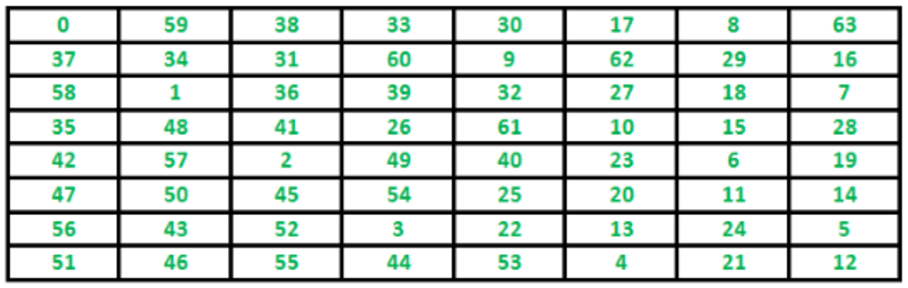
\includegraphics[width=0.8\textwidth]{Images/figGFGBkTSet1KnightsTour}
%\caption[]{}
%\label{figCXNX}
\end{figure}

Let us first discuss the na\"ive algorithm for this problem and then the
Backtracking algorithm.

\rrheader{Naive Algorithm for Knight's tour}

The na\"ive algorithm is to generate all tours one by one and check if the
generated tour satisfies the constraints.
\begin{lstlisting}[style=pseudostyle,numbers=none]
while there are untried tours
{ 
  generate the next tour 
  if this tour covers all squares 
  { 
    print this path;
  }
}
\end{lstlisting}
\textbf{Backtracking} works in an incremental way to attack problems.
Typically, we start from an empty solution vector and one by one add items
(the meaning of item varies from problem to problem. In context of Knight's
tour problem, \textbf{an item} is a \textbf{Knight's move}). When we add an
item, we check if adding the current item violates the problem constraint,
if it does then we remove the item and try other alternatives. \textbf{If
  none of the alternatives work out then we go to previous stage and remove
  the item added in the previous stage.} If we reach the initial stage back
then we say that no solution exists. If adding an item doesn't violate
constraints then we recursively add items one by one. If the solution vector
becomes complete then we print the solution.

\rrheader{Backtracking Algorithm for Knight's tour}

Following is the Backtracking algorithm for Knight's tour problem.
\begin{lstlisting}[style=pseudostyle,numbers=none]
If all squares are visited 
  print the solution
Else
  a) Add one of the next moves to solution vector and recursively 
  check if this move leads to a solution. (A Knight can make maximum 
  eight moves. We choose one of the 8 moves in this step).
  b) If the move chosen in the above step doesn't lead to a solution
  then remove this move from the solution vector and try other 
  alternative moves.
  c) If none of the alternatives work then return false (Returning false 
  will remove the previously added item in recursion and if false is 
  returned by the initial call of recursion then "no solution exists" )
\end{lstlisting}
Following are implementations for Knight's tour problem. It prints one of
the possible solutions in 2D matrix form. Basically, the output is a 2D
$8\times 8$ matrix with numbers from $0$ to $63$ and these numbers show
steps made by Knight.
\begin{lstlisting}[style=raycppnewsnippet]
// C program for Knight Tour problem
#include<stdio.h>
#define N 8
 
int solveKTUtil(int x, int y, int movei, int sol[N][N],
                int xMove[],  int yMove[]);
 
/* A utility function to check if i,j are valid indexes
   for N*N chessboard */
bool isSafe(int x, int y, int sol[N][N])
{
  return (x >= 0 && x < N && y >= 0 &&
          y < N && sol[x][y] == -1);
}
 
/* A utility function to print solution matrix sol[N][N] */
void printSolution(int sol[N][N])
{
  for (int x = 0; x < N; x++)
  {
    for (int y = 0; y < N; y++)
         printf(" %2d ", sol[x][y]);
    printf("\n");
  }
}

/* This function solves the Knight Tour problem using
   Backtracking.  This function mainly uses solveKTUtil()
   to solve the problem. It returns false if no complete
   tour is possible, otherwise return true and prints the
   tour.
   Please note that there may be more than one solutions,
   this function prints one of the feasible solutions.  */
bool solveKT()
{
  int sol[N][N];
 
  /* Initialization of solution matrix */
  for (int x = 0; x < N; x++)
      for (int y = 0; y < N; y++)
          sol[x][y] = -1;
 
  /* xMove[] and yMove[] define next move of Knight.
     xMove[] is for next value of x coordinate
     yMove[] is for next value of y coordinate */
  int xMove[8] = {  2, 1, -1, -2, -2, -1,  1,  2 };
  int yMove[8] = {  1, 2,  2,  1, -1, -2, -2, -1 };
 
  // Since the Knight is initially at the first block
  sol[0][0]  = 0;
 
  /* Start from 0,0 and explore all tours using
     solveKTUtil() */
  if (solveKTUtil(0, 0, 1, sol, xMove, yMove) == false)
  {
    printf("Solution does not exist");
    return false;
  }
  else
    printSolution(sol);
 
  return true;
}

/* A recursive utility function to solve Knight Tour
   problem */
int solveKTUtil(int x, int y, int movei, int sol[N][N],
                int xMove[N], int yMove[N])
{
  int k, next_x, next_y;
  if (movei == N*N)
    return true;
 
  /* Try all next moves from the current coordinate x, y */
  for (k = 0; k < 8; k++)
  {
    next_x = x + xMove[k];
    next_y = y + yMove[k];
    if (isSafe(next_x, next_y, sol))
    {
      sol[next_x][next_y] = movei;
      if (solveKTUtil(next_x, next_y, movei+1, sol,
                      xMove, yMove) == true)
        return true;
      else
        sol[next_x][next_y] = -1;// backtracking
    }
  }
  return false;
}
 
/* Driver program to test above functions */
int main()
{
  solveKT();
  return 0;
}
\end{lstlisting}
Output
\begin{lstlisting}[style=rayio]
  0  59  38  33  30  17   8  63
 37  34  31  60   9  62  29  16
 58   1  36  39  32  27  18   7
 35  48  41  26  61  10  15  28
 42  57   2  49  40  23   6  19
 47  50  45  54  25  20  11  14
 56  43  52   3  22  13  24   5
 51  46  55  44  53   4  21  12
\end{lstlisting}
Note that Backtracking is not the best solution for the Knight's tour
problem. See below article for other better solutions. The purpose of this
post is to explain Backtracking with an example.

Warnsdorff's algorithm for Knight's tour problem (see below).

References:
\begin{itemize}[noitemsep,topsep=0pt]
\item
  http://see.stanford.edu/materials/icspacs106b/H19-RecBacktrackExamples.pdf
\item
  http://www.cis.upenn.edu/~matuszek/cit594-2009/Lectures/35-backtracking.ppt
\item http://mathworld.wolfram.com/KnightsTour.html
\item http://en.wikipedia.org/wiki/Knight\%27s\_tour
\end{itemize}

\textbf{\rrgreen{Recommended: Please try your approach first, before moving
    on to the solution.}}

\RayNotesBegin

Here is my attempt, code here: \path{LeetCode/src/Bcktrck/rrrGFGBcktrckSet1KnightsTour.cpp}
\begin{lstlisting}[style=raycppnewsnippet]
// A utility function to check if (i,j) are valid indices
// for N*N chessboard
bool isLegal(const int x, const int y, const vector<vector<int>>& sol)
{
  auto N = static_cast<int>(sol.size());

  return ((x>=0) && (x<N) && (y>=0) && (y<N) &&
          (sol[x][y] == -1));
}

// A utility function to print a 2D vector
template<typename T>
void print2dVec(const vector<vector<T>>& vec, const string& str="")
{
  if(!str.empty())
  {
    cout << str;
  }

  for(const auto& row:vec)
  {
    for(const auto& val:row)
    {
      cout << std::setw(2) << val << ' ';
    }
    cout << '\n';
  }
}

// A recursive utility function to solve Knight Tour problem.
// curr_x and curr_y are the current x and y positions of the knight
// movei is a count of the current move number.
// sol contains the board.
// xMove and yMove are the new positions of the knight relative to current 
//   pos.
bool solveKTRecur(const int curr_x, const int curr_y, const int movei,
                  vector<vector<int>>& sol,
                  const vector<int>&xMove, const vector<int>&yMove)
{
  //cout << "Doing movei = " << movei << '\n';

  // Base case is when we have filled the whole board.
  // i.e. when movei == N*N
  auto N = static_cast<int>(sol.size());

  // The range of movei = [0..(N*N-1)]. However, for movei=N*N-1, we still
  // want to do the work (filling in the sol, if possible), so we test if
  // movei=N*N and return.
  if(movei == N*N) 
    return true;

  // Now loop through all the possibilities
  for(decltype(xMove.size()) i = 0; i < xMove.size(); ++i)
  {
    // create the next move
    int next_x = curr_x+xMove[i];
    int next_y = curr_y+yMove[i];

    // Check if this position is legal
    if(isLegal(next_x,next_y,sol))
    {
      // We know that we can place the next move here
      sol[next_x][next_y]=movei;

      // Now try every item from here.
      if(solveKTRecur(next_x,next_y,movei+1,
                      sol,xMove,yMove))
      {
        // we get here if we return true all the way down
        return true; 
      }
      else
      {
        // none of the 8 paths from here returns true. So we `backtrack'
        // this move/item and try the next of the 8 moves
        sol[next_x][next_y] = -1;
      }
    } // if legal
  } // for all items/moves

  // If we get here, it means that none of the items/moves worked. So we
  // return false.
  return false;
}

void runSolveKTRecur()
{
  // board size
  int N{8};
  
  // create the board and initialize with -1
  vector<vector<int>> board(N,vector<int>(N,-1));

  // start with the top left.
  int startx=0, starty=0;
  board[startx][starty]=0;

  // Create the eight moves in this order:
  //  2   1
  // 3     0
  //    x
  // 4     7
  //  5   6
  
  /* xMove[] and yMove[] define next move of Knight.
     xMove[] is for next value of x coordinate
     yMove[] is for next value of y coordinate */
  vector<int> xMove{2, 1, -1, -2, -2, -1,  1,  2};
  vector<int> yMove{1, 2,  2,  1, -1, -2, -2, -1};

  // If the solve returns true, it means there's a solution. Otherwise
  // there is no solution.
  if(solveKTRecur(startx,starty,1,board,xMove,yMove))
  {
    print2dVec(board, "Solution is:\n");
  }
  else
  {
    print2dVec(board, "No solution:\n");
    //cout << "Solution does not exist" << '\n';
  }

}

int main()
{
  runSolveKTRecur();

  return 0;
}
\end{lstlisting}

\RayNotesEnd

\textbf{\rrgreen{Back to geeksforgeeks solution.}}

Done, see above.



\subsection{Warnsdorff's algorithm for Knight's tour problem
  \label{secGFGBktrckKnightsTourWarnsdorff}}


RRRTODO

\url{http://www.geeksforgeeks.org/warnsdorffs-algorithm-knights-tour-problem/}

\textbf{Difficulty: 4.7}

\textbf{\rrgreen{Recommended: Please try your approach first, before moving
    on to the solution.}}

\RayNotesBegin



\RayNotesEnd

\textbf{\rrgreen{Back to geeksforgeeks solution.}}


%%%%%%%%%%%%%%%%%%%%%%%%%%%%%%%%%%%%%%%%%%%%%%%%%%%%%%%%%%%%%%%%%%%%%%%%%%%%
%%%%%%%%%%%%%%%%%%%%%%%%%%%%%%%%%%%%%%%%%%%%%%%%%%%%%%%%%%%%%%%%%%%%%%%%%%%%
%%%%%%%%%%%%%%%%%%%%%%%%%%%%%%%%%%%%%%%%%%%%%%%%%%%%%%%%%%%%%%%%%%%%%%%%%%%%

\section{Backtracking | Set 2 (Rat in a Maze)
  \label{secGFGBktrckSet2RatInMaze}}

\url{http://www.geeksforgeeks.org/backttracking-set-2-rat-in-a-maze}

\textbf{Difficulty: 3.2}

We have discussed Backtracking and Knight's tour problem in Set 1
(\pagecref{secGFGBktrckSet1KnightsTour}). Let us discuss Rat in a Maze as
another example problem that can be solved using Backtracking.

A Maze is given as N*N binary matrix of blocks where source block is the
upper left most block i.e., \ctt{maze[0][0]} and destination block is lower
rightmost block i.e., \ctt{maze[N-1][N-1]}. A rat starts from source and has
to reach destination. The rat can move only in two directions: forward and
down.

In the maze matrix, $0$ means the block is dead end and $1$ means the block
can be used in the path from source to destination. Note that this is a
simple version of the typical Maze problem. For example, a more complex
version can be that the rat can move in 4 directions and a more complex
version can be with limited number of moves.

Following is an example maze.

Gray blocks are dead ends (value = $0$). 

\begin{figure}
\centering
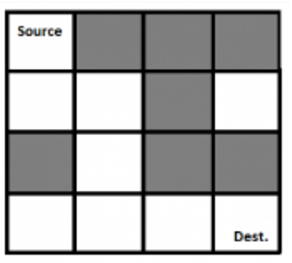
\includegraphics[width=0.3\textwidth]{Images/figGFGBkTSet2RatMaze1}
%\caption[]{}
%\label{figCXNX}
\end{figure}

Following is binary matrix representation of the above maze.
\begin{lstlisting}[style=raygeneric]
                {1, 0, 0, 0}
                {1, 1, 0, 1}
                {0, 1, 0, 0}
                {1, 1, 1, 1}
\end{lstlisting}
Following is maze with highlighted solution path.

\begin{figure}
\centering
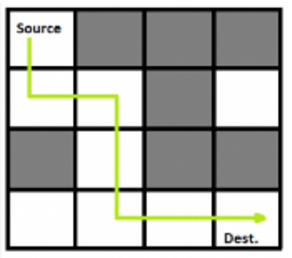
\includegraphics[width=0.3\textwidth]{Images/figGFGBkTSet2RatMaze2}
%\caption[]{}
%\label{figCXNX}
\end{figure}

Following is the solution matrix (output of program) for the above input
matrix.
\begin{lstlisting}[style=raygeneric]
                {1, 0, 0, 0}
                {1, 1, 0, 0}
                {0, 1, 0, 0}
                {0, 1, 1, 1}
\end{lstlisting}
All entries in solution path are marked as $1$.

\textbf{\rrgreen{Recommended: Please try your approach first, before moving
    on to the solution.}}

\RayNotesBegin

So the base case is when $(i,j)==(N-1,N-1)$. If we get to here, we return
\texttt{true}. The items are:
\begin{enumerate}[label=\textbf{\arabic*.}]
\item Go left: $(i,j)=(i+1,j)$.
\item Go down: $(i,j)=(i,j+1)$.
\end{enumerate}
Pseudocode:
\begin{lstlisting}[style=raygeneric]
When we loop through the items, we have to first check if it's legal.
Legal implies: the item is not a wall (value != 0) and is it within the
range of the maze.

  First we set the output value of this item to 1, and:
    Note that only the base case returns true, so we first check if the base
    case can be reached (therefore a solution is found) by recursively
    calling the algo, and propagate that true value back.

    Otherwise, we backtrack this item (set the value of the output to 0) and
    try the next item.

Out of the loop of items: If no true value is returned by any of the items,
we return false.
\end{lstlisting}
Let's code this up: \path{src/Bcktrck/rrrGFGBcktrckSet2RatInMaze.cpp}
\begin{lstlisting}[style=raycppnewsnippet]
template<typename T>
using Grid2d = vector<vector<T>>;

template<typename T>
void printGrid2d(const Grid2d<T>& grid, const string& str = "",
                 const int prec = 0)
{
  if(!str.empty())
    cout << str;

  for(const auto& row:grid)
  {
    for(const auto& val:row)
      cout << std::setw(prec) << val << ' ';
    cout << '\n';
  }
}

bool isLegal(const int x, const int y, const Grid2d<int>& maze)
{
  // size of the maze
  auto N = static_cast<int>(maze.size());

  return ((x >= 0)&&(x<N)&&(y>=0)&&(y<N)&&(maze[x][y] != 0));
}

bool solveMazeRecur(const int curr_x, const int curr_y,
                    const Grid2d<int>& maze,
                    const vector<int>& xmoves, const vector<int>& ymoves,
                    Grid2d<int>& sol)
{
  // size of the maze
  auto N = static_cast<int>(maze.size());

  // base case - solution found!
  if((curr_x == (N-1)) && (curr_y==(N-1)))
    return true;

  // Loop through the items and try each one.
  for(decltype(xmoves.size()) k = 0; k < xmoves.size(); ++k)
  {
    // Get the next position
    int next_x = curr_x + xmoves[k];
    int next_y = curr_y + ymoves[k];

    if(isLegal(next_x,next_y,maze))
    {
      // travel into the next path and ...
      sol[next_x][next_y] = 1;

      // ... try all paths from there
      if(solveMazeRecur(next_x,next_y,maze,xmoves,ymoves,sol))
      {
        return true;
      }
      else
      {
        // un-travel this item `backtracking' and try the next item
        sol[next_x][next_y] = 0;
      }
    }
  }

  // If none of the above child items returns true, then return false, 
  // indicating that this path should not be taken.
  return false;
}

void runSolveMazeRecur()
{
  Grid2d<int>maze{{1, 0, 0, 0},
                  {1, 1, 0, 1},
                  {0, 1, 0, 0},
                  {1, 1, 1, 1}};

  // Solution grid, initialized to 0
  auto N = maze.size();
  Grid2d<int>sol(N,vector<int>(N,0));

  // move vectors (the items), only right and down.
  vector<int> xmoves{1,0};
  vector<int> ymoves{0,1};

  // starting positions: top left.
  int start_x = 0, start_y = 0;
  sol[start_x][start_y] = 1;

  if(solveMazeRecur(start_x,start_y,maze,xmoves,ymoves,sol))
  {
    printGrid2d(sol,"Solution is:\n");
  }
  else
  {
    cout << "No solution.\n";
  }
}
int main()
{
  runSolveMazeRecur();
  return 0;
}
\end{lstlisting}

\RayNotesEnd

\textbf{\rrgreen{Back to geeksforgeeks solution.}}

\rrheader{Na\"ive Algorithm}

The Na\"ive Algorithm is to generate all paths from source to destination
and one by one check if the generated path satisfies the constraints.
\begin{lstlisting}[style=pseudostyle,numbers=none]
while there are untried paths
{
  generate the next path
  if this path has all blocks as 1
  {
    print this path;
  }
}
\end{lstlisting}

\rrheader{Backtrackng Algorithm}

\begin{lstlisting}[style=pseudostyle,numbers=none]
If destination is reached
  print the solution matrix
Else
  a) Mark current cell in solution matrix as 1. 
  b) Move forward in horizontal direction and recursively check if this 
      move leads to a solution. 
  c) If the move chosen in the above step doesn't lead to a solution
      then move down and check if  this move leads to a solution. 
  d) If none of the above solutions work then unmark this cell as 0 
      (BACKTRACK) and return false.
\end{lstlisting}
Implementation of Backtracking solution
\begin{lstlisting}[style=raycppnewsnippet]
/* C/C++ program to solve Rat in a Maze problem using
   backtracking */
#include<stdio.h>
 
// Maze size
#define N 4 
 
bool solveMazeUtil(int maze[N][N], int x, int y, int sol[N][N]);
 
/* A utility function to print solution matrix sol[N][N] */
void printSolution(int sol[N][N])
{
  for (int i = 0; i < N; i++)
  {
    for (int j = 0; j < N; j++)
      printf(" %d ", sol[i][j]);
    printf("\n");
  }
}
 
/* A utility function to check if x,y is valid index for N*N maze */
bool isSafe(int maze[N][N], int x, int y)
{
  // if (x,y outside maze) return false
  if(x >= 0 && x < N && y >= 0 && y < N && maze[x][y] == 1)
    return true;
 
  return false;
}

/* This function solves the Maze problem using Backtracking.  It mainly
   uses solveMazeUtil() to solve the problem. It returns false if no 
   path is possible, otherwise return true and prints the path in the
   form of 1s. Please note that there may be more than one solutions, 
   this function prints one of the feasible solutions.*/
bool solveMaze(int maze[N][N])
{
  int sol[N][N] = { {0, 0, 0, 0},
      {0, 0, 0, 0},
      {0, 0, 0, 0},
      {0, 0, 0, 0}
  };
 
  if(solveMazeUtil(maze, 0, 0, sol) == false)
  {
    printf("Solution doesn't exist");
    return false;
  }
 
  printSolution(sol);
  return true;
}

/* A recursive utility function to solve Maze problem */
bool solveMazeUtil(int maze[N][N], int x, int y, int sol[N][N])
{
  // if (x,y is goal) return true
  if(x == N-1 && y == N-1)
  {
    sol[x][y] = 1;
    return true;
  }
 
  // Check if maze[x][y] is valid
  if(isSafe(maze, x, y) == true)
  {
    // mark x,y as part of solution path
    sol[x][y] = 1;
 
    /* Move forward in x direction */
    if (solveMazeUtil(maze, x+1, y, sol) == true)
      return true;
 
    /* If moving in x direction doesn't give solution then
       Move down in y direction  */
    if (solveMazeUtil(maze, x, y+1, sol) == true)
      return true;
 
    /* If none of the above movements work then BACKTRACK: 
        unmark x,y as part of solution path */
    sol[x][y] = 0;
    return false;
  }   
 
  return false;
}

// driver program to test above function
int main()
{
  int maze[N][N]  =  { {1, 0, 0, 0},
                       {1, 1, 0, 1},
                       {0, 1, 0, 0},
                       {1, 1, 1, 1}};
 
  solveMaze(maze);
  return 0;
}
\end{lstlisting}
Output: The 1 values show the path for rat
\begin{lstlisting}[style=rayio]
 1  0  0  0 
 1  1  0  0 
 0  1  0  0 
 0  1  1  1 
\end{lstlisting}
Below is an extended version of this problem. Count number of ways to reach
destination in a Maze

%%%%%%%%%%%%%%%%%%%%%%%%%%%%%%%%%%%%%%%%%%%%%%%%%%%%%%%%%%%%%%%%%%%%%%%%%%%%
%%%%%%%%%%%%%%%%%%%%%%%%%%%%%%%%%%%%%%%%%%%%%%%%%%%%%%%%%%%%%%%%%%%%%%%%%%%%
%%%%%%%%%%%%%%%%%%%%%%%%%%%%%%%%%%%%%%%%%%%%%%%%%%%%%%%%%%%%%%%%%%%%%%%%%%%%

\subsection{Count number of ways to reach destination in a Maze
  \label{secGFGBktrckCountWaysMaze}}

\url{https://www.geeksforgeeks.org/count-number-ways-reach-destination-maze}

\textbf{Difficulty: 3.1}

RRRTODO


\textbf{\rrgreen{Recommended: Please try your approach first, before moving
    on to the solution.}}

\RayNotesBegin



\RayNotesEnd

\textbf{\rrgreen{Back to geeksforgeeks solution.}}


%%%%%%%%%%%%%%%%%%%%%%%%%%%%%%%%%%%%%%%%%%%%%%%%%%%%%%%%%%%%%%%%%%%%%%%%%%%%
%%%%%%%%%%%%%%%%%%%%%%%%%%%%%%%%%%%%%%%%%%%%%%%%%%%%%%%%%%%%%%%%%%%%%%%%%%%%
%%%%%%%%%%%%%%%%%%%%%%%%%%%%%%%%%%%%%%%%%%%%%%%%%%%%%%%%%%%%%%%%%%%%%%%%%%%%

\section{Backtracking | Set 3 (N Queen Problem)
  \label{secGFGBktrckSet3NQueenProb}}

\url{http://www.geeksforgeeks.org/backtracking-set-3-n-queen-problem}

\textbf{Difficulty: 3.5}

We have discussed Knight's tour and Rat in a Maze problems in Set 1
(\pagecref{secGFGBktrckSet1KnightsTour}) and Set 2
(\pagecref{secGFGBktrckSet2RatInMaze}) respectively. Let us discuss N Queen
as another example problem that can be solved using Backtracking.

The N Queen is the problem of placing $N$ chess queens on an $N\times N$
chessboard so that no two queens attack each other. For example, following
is a solution for $4$ Queen problem.

\begin{figure}
\centering
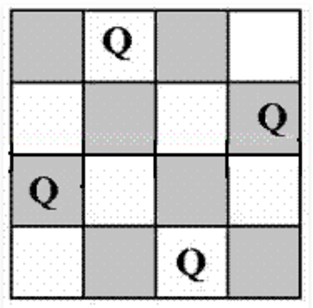
\includegraphics[width=0.25\textwidth]{Images/figGFGBkTSet3NQueen}
%\caption[]{}
%\label{figCXNX}
\end{figure}

The expected output is a binary matrix which has $1$s for the blocks where
queens are placed. For example following is the output matrix for above $4$
queen solution.
\begin{lstlisting}[style=raygeneric]
              { 0,  1,  0,  0}
              { 0,  0,  0,  1}
              { 1,  0,  0,  0}
              { 0,  0,  1,  0}
\end{lstlisting}

\textbf{\rrgreen{Recommended: Please try your approach first, before moving
    on to the solution.}}

\RayNotesBegin

Okay, let's recall what we know about backtracking.
\begin{itemize}[noitemsep,topsep=0pt]
\item We need to come up with the items/actions to take per recursive level.
\item We need to come up with the base case.
\item We need to come up with the restriction, which may depends on the
  previously places solution. This is usually handled by the \ctt{isLegal}
  method.
\end{itemize}

\textbf{Base case:} Easy, it's when we have placed $N$ queens on the board.

For the items, we need to use some logic. Let's place the first queen on the
top left, at $(i=0,j=0)$. Note that this is not fixed, so for the next
items, we can choose to place the queen (the initial one) at each of the
empty squares in row major order, and check if it's \emph{valid}. However,
we can do better. We know that since there are $N$ queens, and the board is
$N\times N$, then \textbf{each queen must be on its own column}.

Thus, we can work through the columns, for each column, the items are the
number of rows. We must check all rows, since the previously placed queens
may have moved (backtracked) to a different row. Say we work through the
columns from left to right, then to check if a square is valid, we only need
to check squares to the left:
\begin{itemize}[noitemsep,topsep=0pt]
\item Check squares to the left and see if there are no queens.
\item Check diagonal going up.
\item Check diagonal going down.
\end{itemize}
Thus, the pseudocode is something like this:
\begin{lstlisting}[style=pseudostyle,numbers=none]
bool solveNQueen(int col, grid sol[][])
{
  // We try to place the col-th queen. If col = sol.size(), then we know
  // that we have already placed all the N queens in the 0..N-1 columns.
  if(col == N)
    return true

  // Try to place the queen in the col-th column by looping throught the
  // rows
  Loop through rows
    if (row,col) is legal
      a) set the queen here: sol[row][col] = 1
      b) Go depth-first, recursively place the remaining queens, and
      propagate true back if a solution is reached.
      c) If it's not possible, then `backtrack' (reset) this row
         sol[row][col]=0
      and let the loop go for the next row.
    end if
  end loop through rows

  // If none of the rows work, return false.
  return false
}
\end{lstlisting}
Let's code this up: \path{Bcktrck/rrrGFGBcktrckSet3NQueen.cpp}
\begin{lstlisting}[style=raycppnewsnippet]
template<typename T>
using Grid2d = vector<vector<T>>;

template<typename T>
void printGrid2d(const Grid2d<T>& board)
{
  for(const auto& row:board)
  {
    for(const auto& val:row)
    {
      cout << val << ' ';
    }
    cout << '\n';
  }
}

// Check to see if x and y are within the board (0<=x,y<N-1) and 
// 1) Check left horizontally
// 2) Check up diagonal
// 3) Check down diagonal
bool isLegal(const int x, const int y, const Grid2d<int>& board)
{
  // First check if x and y are in range
  auto N = static_cast<int>(board.size());
  if(x < 0 || x>=N || y<0 || y>= N)
  {
    return false;
  }

  // Check if to the left, so only column changes
  for(int yi = 0; yi < y; ++yi)
    if(board[x][yi] == 1)
      return false;

  // Check if up diag, both row and col indices reduce by 1 at each 
  // iteration
  for(int xi = x, yi = y; xi >= 0 && yi >= 0; xi--, yi--)
    if(board[xi][yi]==1)
      return false;

  // Check if down diag, row increases by 1, col decreases by 1
  for(int xi = x, yi = y; xi < N && yi >= 0; ++xi, --yi)
    if(board[xi][yi]==1)
      return false;

  return true;
}

bool solveNQueenRecur(const int col, Grid2d<int>& board)
{
  // We try to place the col-th queen in the col-th column. 
  // If col == board.size(), then we know that we have already placed all 
  // the N queens in the 0..N-1 columns
  auto N = static_cast<int>(board.size());
  if(col == N)
    return true;

  // Try to place the queen in the col-th column by looping through the rows
  for(int row = 0; row < N; ++row)
  {
    if(isLegal(row,col,board))
    {
      // Found a legal square, so we set the queen here
      board[row][col] = 1;
      
      // Now try for the next column. We go deeper, depth-first,
      // recursively placing the remaining queens, and propagate true back
      // to the caller of this function if the base case is reached.
      if(solveNQueenRecur(col+1,board))
        return true;
      else
        // backtrack by resetting (row,col) to zero, so we can try a 
        // different row.
        board[row][col] = 0;
    }
  }

  // If none of the rows work=>none of the path of items , return false
  return false;
}

void runSolveNQueens()
{
  constexpr size_t N = 100;
  Grid2d<int> board(N,vector<int>(N,0));
  solveNQueenRecur(0,board);
  printGrid2d(board);
}

int main()
{
  runSolveNQueens();
  return 0;
}
\end{lstlisting}

\RayNotesEnd

\textbf{\rrgreen{Back to geeksforgeeks solution.}}

\rrheader{Naive Algorithm}

Generate all possible configurations of queens on board and print a
configuration that satisfies the given constraints.
\begin{lstlisting}[style=pseudostyle,numbers=none]
while there are untried conflagrations
{
  generate the next configuration
  if queens don't attack in this configuration then
  {
    print this configuration;
  }
}
\end{lstlisting}

\rrheader{Backtracking Algorithm}

The idea is to place queens one by one in different columns, starting from
the leftmost column. When we place a queen in a column, we check for clashes
with already placed queens. In the current column, if we find a row for
which there is no clash, we mark this row and column as part of the
solution. If we do not find such a row due to clashes then we backtrack and
return \texttt{false}.
\begin{lstlisting}[style=raygeneric]
1) Start in the leftmost column
2) If all queens are placed
    return true
3) Try all rows in the current column.  Do following for every tried row.
    a) If the queen can be placed safely in this row then mark this [row, 
        column] as part of the solution and recursively check if placing  
        queen here leads to a solution.
    b) If placing queen in [row, column] leads to a solution then return 
        true.
    c) If placing queen doesn't lead to a solution then umark this [row, 
        column] (Backtrack) and go to step (a) to try other rows.
3) If all rows have been tried and nothing worked, return false to trigger 
    backtracking.
\end{lstlisting}

\rrheader{Implementation of Backtracking solution}

\begin{lstlisting}[style=raycppnewsnippet]
/* C/C++ program to solve N Queen Problem using
   backtracking */
#define N 4
#include<stdio.h>
 
/* A utility function to print solution */
void printSolution(int board[N][N])
{
  for (int i = 0; i < N; i++)
  {
    for (int j = 0; j < N; j++)
      printf(" %d ", board[i][j]);
    printf("n");
  }
}

/* A utility function to check if a queen can
   be placed on board[row][col]. Note that this
   function is called when "col" queens are
   already placed in columns from 0 to col -1.
   So we need to check only left side for
   attacking queens */
bool isSafe(int board[N][N], int row, int col)
{
  int i, j;
 
  /* Check this row on left side */
  for (i = 0; i < col; i++)
    if (board[row][i])
      return false;
 
  /* Check upper diagonal on left side */
  for (i=row, j=col; i>=0 && j>=0; i--, j--)
    if (board[i][j])
      return false;
 
  /* Check lower diagonal on left side */
  for (i=row, j=col; j>=0 && i<N; i++, j--)
    if (board[i][j])
      return false;
 
  return true;
}

/* A recursive utility function to solve N
   Queen problem */
bool solveNQUtil(int board[N][N], int col)
{
  /* base case: If all queens are placed
    then return true */
  if (col >= N)
    return true;
 
  /* Consider this column and try placing
     this queen in all rows one by one */
  for (int i = 0; i < N; i++)
  {
    /* Check if queen can be placed on
      board[i][col] */
    if ( isSafe(board, i, col) )
    {
      /* Place this queen in board[i][col] */
      board[i][col] = 1;
 
      /* recur to place rest of the queens */
      if ( solveNQUtil(board, col + 1) )
        return true;
 
      /* If placing queen in board[i][col]
         doesn't lead to a solution, then
         remove queen from board[i][col] */
      board[i][col] = 0; // BACKTRACK
    }
  }
 
   /* If queen can not be place in any row in
      this colum col  then return false */
  return false;
}

/* This function solves the N Queen problem using
   Backtracking. It mainly uses solveNQUtil() to
   solve the problem. It returns false if queens
   cannot be placed, otherwise return true and
   prints placement of queens in the form of 1s.
   Please note that there may be more than one
   solutions, this function prints one  of the
   feasible solutions.*/
bool solveNQ()
{
  int board[N][N] = { {0, 0, 0, 0},
      {0, 0, 0, 0},
      {0, 0, 0, 0},
      {0, 0, 0, 0}
  };
 
  if ( solveNQUtil(board, 0) == false )
  {
    printf("Solution does not exist");
    return false;
  }
 
  printSolution(board);
  return true;
}
 
// driver program to test above function
int main()
{
  solveNQ();
  return 0;
}
\end{lstlisting}
Output: The 1 values indicate placements of queens
\begin{lstlisting}[style=rayio]
 0  0  1  0 
 1  0  0  0 
 0  0  0  1 
 0  1  0  0 
\end{lstlisting}

Sources:
\begin{itemize}[noitemsep,topsep=0pt]
\item
  http://see.stanford.edu/materials/icspacs106b/H19-RecBacktrackExamples.pdf
\item http://en.literateprograms.org/Eight\_queens\_puzzle\_\%28C\%29
\item http://en.wikipedia.org/wiki/Eight\_queens\_puzzle
\end{itemize}

%%%%%%%%%%%%%%%%%%%%%%%%%%%%%%%%%%%%%%%%%%%%%%%%%%%%%%%%%%%%%%%%%%%%%%%%%%%%
%%%%%%%%%%%%%%%%%%%%%%%%%%%%%%%%%%%%%%%%%%%%%%%%%%%%%%%%%%%%%%%%%%%%%%%%%%%%
%%%%%%%%%%%%%%%%%%%%%%%%%%%%%%%%%%%%%%%%%%%%%%%%%%%%%%%%%%%%%%%%%%%%%%%%%%%%

\subsection{Printing all solutions in N-Queens Problem}

\url{https://www.geeksforgeeks.org/printing-solutions-n-queen-problem}

\textbf{Difficulty: 3.6}

The N Queen is the problem of placing N chess queens on an $N\times N$
chessboard so that no two queens attack each other. For example, following
is a solution for 4 Queen problem.

The N Queen is the problem of placing N chess queens on an $N\times N$
chessboard so that no two queens attack each other. For example, following
is a solution for 4 Queen problem.

\begin{figure}
\centering
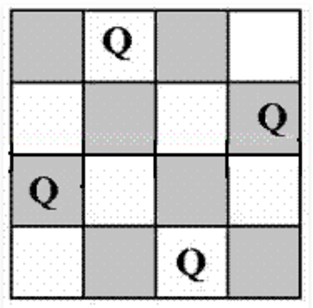
\includegraphics[width=0.25\textwidth]{Images/figGFGBkTSet3NQueen}
%\caption[]{}
%\label{figCXNX}
\end{figure}

In previous post, we have discussed an approach that prints only one
possible solution, so now in this post the task is to print all solutions in
N-Queen Problem. The solution discussed here is an extension of same
approach.

\textbf{\rrgreen{Recommended: Please try your approach first, before moving
    on to the solution.}}

\RayNotesBegin

RRRTODO - it seems pretty easy. It's literally looping through all the
rows rather than returning at the first sight of a solution. And we always
backtrack. This seems more like a brute force approach than anything else.

\RayNotesEnd

\textbf{\rrgreen{Back to geeksforgeeks solution.}}



%%%%%%%%%%%%%%%%%%%%%%%%%%%%%%%%%%%%%%%%%%%%%%%%%%%%%%%%%%%%%%%%%%%%%%%%%%%%
%%%%%%%%%%%%%%%%%%%%%%%%%%%%%%%%%%%%%%%%%%%%%%%%%%%%%%%%%%%%%%%%%%%%%%%%%%%%
%%%%%%%%%%%%%%%%%%%%%%%%%%%%%%%%%%%%%%%%%%%%%%%%%%%%%%%%%%%%%%%%%%%%%%%%%%%%

\section{Backtracking | Set 4 (Subset Sum)
  \label{secGFGBktrckSet4SubsetSum}}

\url{http://www.geeksforgeeks.org/backttracking-set-4-subset-sum}

\textbf{Difficulty: 4.4}

Subset sum problem is to find subset of elements that are selected from a
given set whose sum adds up to a given number $K$. We are considering the
set contains non-negative values. It is assumed that the input set is unique
(no duplicates are presented).

\textbf{\rrgreen{Recommended: Please try your approach first, before moving
    on to the solution.}}

\RayNotesBegin

I really don't this the backtracking solution to this atm. So I'll just go
onto the solution. However, note that this can be easily solved by DP, it's
basically an integer partitioning. We have a sum, and have to partition it
into some subset of integers, see this:\\
\url{https://www.geeksforgeeks.org/dynamic-programming-subset-sum-problem}

\RayNotesEnd

\textbf{\rrgreen{Back to geeksforgeeks solution.}}

\rrheader{Exhaustive Search Algorithm for Subset Sum}

One way to find subsets that sum to $K$ is to consider all possible subsets.
A power set contains all those subsets generated from a given set. The size
of such a power set is $2^N$.

\rrheader{Backtracking Algorithm for Subset Sum}

Using exhaustive search we consider all subsets irrespective of whether they
satisfy given constraints or not. Backtracking can be used to make a
systematic consideration of the elements to be selected.

\rrblue{(But how do we select them using backtracking? What are the "items"
  - how do we generate them?)}

Assume given set of $4$ elements, say $w[1]\ldots w[4]$. Tree diagrams can
be used to design backtracking algorithms. The following tree diagram
depicts approach of generating variable sized tuple.

\begin{figure}
\centering
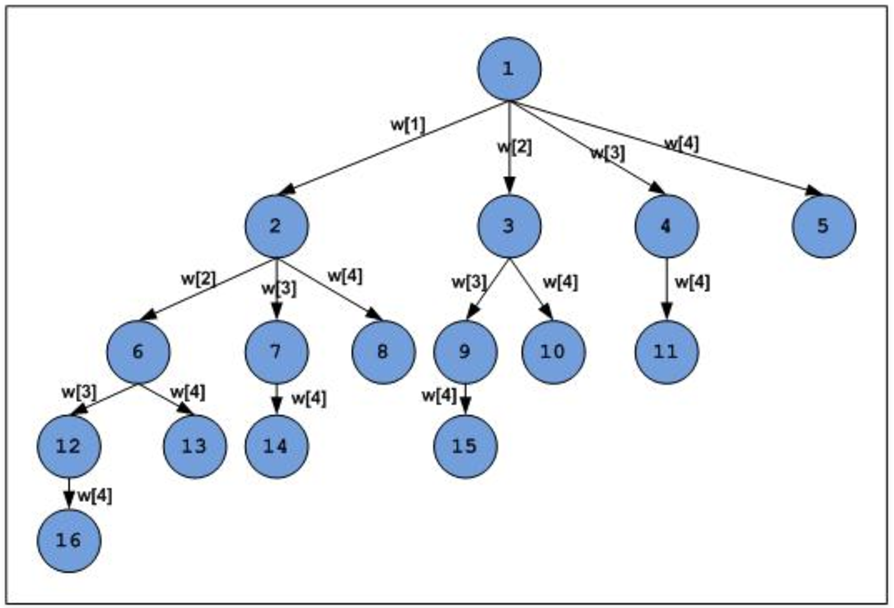
\includegraphics[width=0.8\textwidth]{Images/figGFGBkTSet4SubsetSum}
%\caption[]{}
%\label{figCXNX}
\end{figure}

In the above tree, a node represents function call and a branch represents
candidate element. The root node contains 4 children. In other words, the
root considers every element of the set as different branch. The next level
\textbf{sub-trees} correspond to the subsets that includes the parent node.
The branches at each level represent tuple elements to be considered. For
example, if we are at level 1, \ctt{tuple\_vector[1]} can take any value of
four branches generated. If we are at level 2 of left most node,
\ctt{tuple\_vector[2]} can take any value of three branches generated, and
so on...

For example the left most child of the root generates all those subsets that
include \ctt{w[1]}. Similarly the second child of root generates all those
subsets that includes \ctt{w[2]} \textbf{and excludes} \ctt{w[1]}.

As we go down along depth of tree we add elements so far, and if the added
sum is satisfying \textbf{explicit constraints}, we will continue to
generate child nodes further. Whenever the constraints are not met, we stop
further generation of sub-trees of that node, and backtrack to previous node
to explore the nodes not yet explored. In many scenarios, it saves
considerable amount of processing time.

The tree should trigger a clue to implement the backtracking algorithm (try
yourself). It prints all those subsets whose sum add up to given number. We
need to explore the nodes along the breadth and depth of the tree.
Generating nodes along breadth is controlled by loop and nodes along the
depth are generated using recursion (post order traversal). Pseudo code
given below,
\begin{lstlisting}[style=raygeneric]
if(subset is satisfying the constraint)
  print the subset
  exclude the current element and consider next element
else
  generate the nodes of present level along breadth of tree and
  recur for next levels
\end{lstlisting}
Following is C implementation of subset sum using variable size tuple
vector. Note that the following program explores all possibilities similar
to exhaustive search. It is to demonstrate how backtracking can be used. See
next code to verify, how we can optimize the backtracking solution.

For my attempt see here:\\
\path{src/Bcktrck/rrrGFGBcktrckSet4SubsetSum.cpp}\\
also see their solution at:\\
\path{src/Bcktrck/rrrGFGBcktrckSet4Test.cpp}\\

I'll come back to this, since I cba... it jut seems a bit weird.

RRRTODO

%%%%%%%%%%%%%%%%%%%%%%%%%%%%%%%%%%%%%%%%%%%%%%%%%%%%%%%%%%%%%%%%%%%%%%%%%%%%
%%%%%%%%%%%%%%%%%%%%%%%%%%%%%%%%%%%%%%%%%%%%%%%%%%%%%%%%%%%%%%%%%%%%%%%%%%%%
%%%%%%%%%%%%%%%%%%%%%%%%%%%%%%%%%%%%%%%%%%%%%%%%%%%%%%%%%%%%%%%%%%%%%%%%%%%%

\section{Backtracking | Set 5 (m Coloring Problem)
  \label{secGFGBktrckSet5mColorProb}}

\url{http://www.geeksforgeeks.org/backttracking-set-5-m-coloring-problem}

\textbf{Difficulty: 3.6}

Given an undirected graph and a number $m$, determine if the graph can be
colored with at most $m$ colors such that no two adjacent vertices of the
graph are colored with same color. Here coloring of a graph means assignment
of colors to all vertices.

\noindent{}\textbf{Input:}\\
\begin{enumerate}[label=\textbf{\arabic*.}]
\item A 2D array \ctt{graph[V][V]} where $V$ is the number of vertices in
  graph and \ctt{graph[V][V]} is adjacency matrix representation of the
  graph. A value \ctt{graph[i][j]} is $1$ if there is a direct edge from $i$
  to $j$, otherwise \ctt{graph[i][j]} is $0$.
\item An integer $m$ which is maximum number of colors that can be used.
\end{enumerate}

\noindent{}\textbf{Output:}\\
An array \ctt{color[V]} that should have numbers from $1$ to $m$.
\ctt{color[i]} should represent the color assigned to the $i$th vertex. The
code should also return false if the graph cannot be colored with $m$
colors.

Following is an example graph (from Wiki page ) that can be colored with 3
colors.

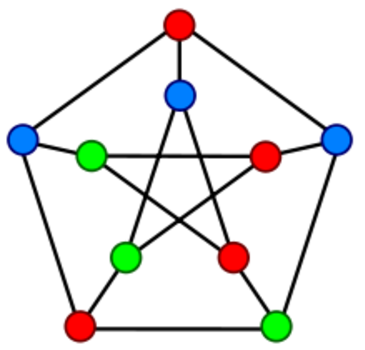
\includegraphics[width=0.3\textwidth]{Images/figGFGBkTSet5GraphColor}

\textbf{\rrgreen{Recommended: Please try your approach first, before moving
    on to the solution.}}

\RayNotesBegin

When you can't think of a solution or approach to a problem, it might help
to come up with the brute-force solution, and then maybe a simpler example,
a reduced problem.

\noindent{}\textbf{Brute force:} Try every combination of colouring, and
check which one satisfies the constraint. Since each node can be one of $m$
colours, so there are $m^N$ different combinations of colouring, where $N$
is the number of nodes in the graph (i.e. if there are only 2 colours, then
it's $2^N$, which is the same as the number of different combinations of
binary numbers of $N$ bits).

So trying each combination of colours is the ``item'', which spans the
breadth. We start at node $i=0$, and set it to a color $color[i]=c, c\in
[1..m]$, check if it's legal. Legal means that no other node in the
adjacency matrix has the same color as color $c$. If it's legal, then we
recursively try to update $color[i+1]$. If not, we backtrack, setting
\ctt{color[i]=0} and trying the next color in the loop.

Let's code this up:
\begin{lstlisting}[style=raycppnewsnippet]
template<typename T>
using Grid2d = vector<vector<T>>;

// function to output a vector
template<typename T>
void printVec(vector<T>& v, const string& str="")
{
  if(!str.empty()) cout << str;
  for(const auto& val:v)
    cout << val << " ";
  cout << '\n';
}

// a color m_index is legal for nodei is no other node in graph[nodei] has
// the same color
bool isLegal(const int nodei, const int m_index, 
             const Grid2d<int>& graph, const vector<int>& color)
{
  // Loop through the nodes, if they are adjacent to node i, check if
  // it has been assigned a color the same as color[m_index]
  for(size_t i = 0; i < graph.size(); ++i)
    if(graph[nodei][i] && (m_index==color[i]))
      return false;
  
  return true;
}

bool solveMColor(const Grid2d<int>& graph, const int m, const int nodei, 
                  vector<int>& color)
{
  // base case is when we have coloured all the nodes, i.e.
  // when nodei = color.size()
  if(nodei == color.size())
    return true;

  // For this node, loop through the colors, backtrack is necessary 
  // (breadth-first).
  // Recursively call solveMColor for node+1 (depth-first)
  for(int m_index = 1; m_index <= m; m_index++)
  {
    if(isLegal(nodei, m_index, graph, color))
    {
      color[nodei] = m_index;
      if(solveMColor(graph, m, nodei+1, color))
        return true;

      // backtrack
      color[nodei] = 0;
    }
  }

  return false;
}

void runSolveMColor()
{
  Grid2d<int> grid{{0,1,1,1},
                   {1,0,1,0},
                   {1,1,0,1},
                   {1,0,1,0}};

  int m = 3;
  vector<int> color(grid.size(),0);

  if(solveMColor(grid, m, 0, color))
    printVec(color,"Solution is:\n");
  else
    cout << "No sol" << '\n';
}

int main()
{
  runSolveMColor();
  return 0;
}
\end{lstlisting}

\RayNotesEnd

\textbf{\rrgreen{Back to geeksforgeeks solution.}}

\rrheader{Naive Algorithm}

Generate all possible configurations of colors and print a configuration
that satisfies the given constraints.
\begin{lstlisting}[style=raycppnewsnippet]
while there are untried conflagrations
{
  generate the next configuration
  if no adjacent vertices are colored with same color
  {
    print this configuration;
  }
}
\end{lstlisting}
There will be $m^V$ configurations of colors.

\rrheader{Backtracking Algorithm}

The idea is to assign colors one by one to different vertices, starting from
the vertex $0$. Before assigning a color, we check for safety by considering
already assigned colors to the adjacent vertices. If we find a color
assignment which is safe, we mark the color assignment as part of solution.
If we do not a find color due to clashes then we backtrack and return
\texttt{false}.

Implementation of Backtracking solution
\begin{lstlisting}[style=raycppnewsnippet]
#include<stdio.h>
 
// Number of vertices in the graph
#define V 4
 
void printSolution(int color[]);
 
/* A utility function to check if the current color assignment
   is safe for vertex v */
bool isSafe (int v, bool graph[V][V], int color[], int c)
{
  for (int i = 0; i < V; i++)
    if (graph[v][i] && c == color[i])
      return false;
  return true;
}
 
/* A recursive utility function to solve m coloring problem */
bool graphColoringUtil(bool graph[V][V], int m, int color[], int v)
{
  /* base case: If all vertices are assigned a color then
       return true */
  if (v == V)
    return true;
 
  /* Consider this vertex v and try different colors */
  for (int c = 1; c <= m; c++)
  {
    /* Check if assignment of color c to v is fine*/
    if (isSafe(v, graph, color, c))
    {
      color[v] = c;

      /* recur to assign colors to rest of the vertices */
      if (graphColoringUtil (graph, m, color, v+1) == true)
        return true;
 
      /* If assigning color c doesn't lead to a solution
         then remove it */
      color[v] = 0;
    }
  }
 
  /* If no color can be assigned to this vertex then return false */
  return false;
}
 
/* This function solves the m Coloring problem using Backtracking.
  It mainly uses graphColoringUtil() to solve the problem. It returns
  false if the m colors cannot be assigned, otherwise return true and
  prints assignments of colors to all vertices. Please note that there
  may be more than one solutions, this function prints one of the
  feasible solutions.*/
bool graphColoring(bool graph[V][V], int m)
{
  // Initialize all color values as 0. This initialization is needed
  // correct functioning of isSafe()
  int *color = new int[V];
  for (int i = 0; i < V; i++)
    color[i] = 0;
 
  // Call graphColoringUtil() for vertex 0
  if (graphColoringUtil(graph, m, color, 0) == false)
  {
    printf("Solution does not exist");
    return false;
  }
 
  // Print the solution
  printSolution(color);
  return true;
}
 
/* A utility function to print solution */
void printSolution(int color[])
{
  printf("Solution Exists:"
         " Following are the assigned colors \n");
  for (int i = 0; i < V; i++)
    printf(" %d ", color[i]);
  printf("\n");
}
 
// driver program to test above function
int main()
{
  /* Create following graph and test whether it is 3 colorable
    (3)---(2)
     |   / |
     |  /  |
     | /   |
    (0)---(1)
  */
  bool graph[V][V] = {{0, 1, 1, 1},
                      {1, 0, 1, 0},
                      {1, 1, 0, 1},
                      {1, 0, 1, 0},
                     };
  int m = 3; // Number of colors
  graphColoring (graph, m);
  return 0;
}
\end{lstlisting}
Output:
\begin{lstlisting}[style=rayio]
Solution Exists: Following are the assigned colors
 1  2  3  2
\end{lstlisting}
References:
\url{http://en.wikipedia.org/wiki/Graph\_coloring}

%%%%%%%%%%%%%%%%%%%%%%%%%%%%%%%%%%%%%%%%%%%%%%%%%%%%%%%%%%%%%%%%%%%%%%%%%%%%
%%%%%%%%%%%%%%%%%%%%%%%%%%%%%%%%%%%%%%%%%%%%%%%%%%%%%%%%%%%%%%%%%%%%%%%%%%%%
%%%%%%%%%%%%%%%%%%%%%%%%%%%%%%%%%%%%%%%%%%%%%%%%%%%%%%%%%%%%%%%%%%%%%%%%%%%%

\section{Backtracking | Set 6 (Hamiltonian Cycle)
  \label{secGFGBktrckSet6HamiltonianCycle}}

\url{http://www.geeksforgeeks.org/backtracking-set-7-hamiltonian-cycle}

\textbf{Difficulty: 3.7}

\textbf{\emph{Hamiltonian
    Path}}\footnote{\url{http://en.wikipedia.org/wiki/Hamiltonian\_path}}
in an undirected graph is a path that \textbf{visits each vertex exactly
  once}. A \textbf{\emph{Hamiltonian cycle}} (or Hamiltonian circuit) is a
Hamiltonian Path such that there is an edge (in the graph) from the last
vertex to the first vertex of the Hamiltonian Path. Determine whether a
given graph contains Hamiltonian Cycle or not. If it contains, then print
the path. Following are the input and output of the required function.

\noindent{}\textbf{Input:}\\
A 2D array \ctt{graph[V][V]} where $V$ is the number of vertices in the
graph and \ctt{graph[V][V]} is adjacency matrix representation of the graph.
A value \ctt{graph[i][j]} is $1$ if there is a direct edge from $i$ to $j$,
otherwise \ctt{graph[i][j]} is $0$.

\noindent{}\textbf{Output:}\\ An array \ctt{path[V]} that should contain the
Hamiltonian Path.  \ctt{path[i]} should represent the $i$th vertex in the
Hamiltonian Path. The code should also return \texttt{false} if there is no
Hamiltonian Cycle in the graph.

For example, a Hamiltonian Cycle in the following graph is
$\set*{0,1,2,4,3,0}$. There are more Hamiltonian Cycles in the graph like
$\set*{0,3,4,2,1,0}$
\begin{lstlisting}[style=raygeneric]
(0)--(1)--(2)
 |   / \   |
 |  /   \  | 
 | /     \ |
(3)-------(4)
\end{lstlisting}
And the following graph doesn't contain any Hamiltonian Cycle.
\begin{lstlisting}[style=raygeneric]
(0)--(1)--(2)
 |   / \   |
 |  /   \  | 
 | /     \ |
(3)      (4) 
\end{lstlisting}

\textbf{\rrgreen{Recommended: Please try your approach first, before moving
    on to the solution.}}

\RayNotesBegin

This is a bit more complicated than the last one since there is an
additional condition on the last node (it has to be adjacent to the first
node).

First, let's jot some notes down, then describe the naive approach.
\begin{itemize}[noitemsep,topsep=0pt]
\item The choices of nodes are the items in this case.
\item We start with node $0$, this is justified since we're forming a cycle,
  so it does not matter where we start. This is what we start the recursion
  with.
\item At each node (level of recursion) (this is the breadth-first stage),
  we loop through the node's adjacency list, generating the breadth-first
  items.
\item For each of the breadth-first items (adjacency nodes), we check if
  it's \textbf{legal}. In this case, legal means that we have not visited
  the node already. This is easily done since we have a list of nodes we
  have visited in the array \ctt{path[V]}, thus we simply which if the node
  we're going to add to the \ctt{path} is not already in \ctt{path}.
\item For the \textbf{base case}, we do not simply check if we have
  \textbf{already} added all the nodes to \ctt{path}. (For which we check if
  the node we're trying to add is equal to the number of nodes). Instead, we
  check if check if this is the last node to be added (nodei==V-1), if so,
  we check if the first node is in the adjacency list of nodei. If it is,
  then we're done, return \texttt{true}. If not, then a cycle cannot be
  formed on this path, so we return \texttt{false}.
\end{itemize}

Let's code this up!
Done, but with a small bug with I cba to find. The code is here:\\
\path{src/Bcktrck/rrrGFGBcktrckSet6Hamiltonian.cpp}

\RayNotesEnd

\textbf{\rrgreen{Back to geeksforgeeks solution.}}





%%%%%%%%%%%%%%%%%%%%%%%%%%%%%%%%%%%%%%%%%%%%%%%%%%%%%%%%%%%%%%%%%%%%%%%%%%%%
%%%%%%%%%%%%%%%%%%%%%%%%%%%%%%%%%%%%%%%%%%%%%%%%%%%%%%%%%%%%%%%%%%%%%%%%%%%%
%%%%%%%%%%%%%%%%%%%%%%%%%%%%%%%%%%%%%%%%%%%%%%%%%%%%%%%%%%%%%%%%%%%%%%%%%%%%

\section{Backtracking | Set 7 Sudoku
  \label{secGFGBktrckSet7Sudoku}}

\url{http://www.geeksforgeeks.org/backtracking-set-7-suduku}

\textbf{Difficulty: 3.8}

Given a partially filled $9\times 9$ 2D array `\ctt{grid[9][9]}', the goal
is to assign digits (from $1$ to $9$) to the empty cells so that every row,
column, and subgrid of size $3\times 3$ contains exactly one instance of the
digits from $1$ to $9$.

\begin{figure}
\centering
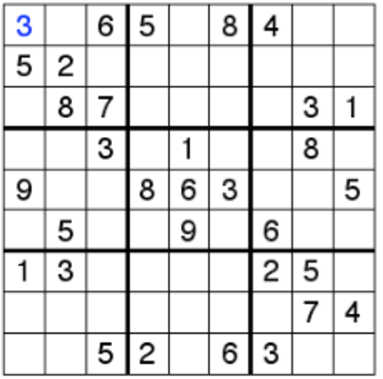
\includegraphics[width=0.3\textwidth]{Images/figGFGBkTSet7Sudoku}
%\caption[]{}
%\label{figCXNX}
\end{figure}

\textbf{\rrgreen{Recommended: Please try your approach first, before moving
    on to the solution.}}

\RayNotesBegin

I'll do it alongside the solution to save time. This seems pretty easy. It's
standard backtracking.

\RayNotesEnd

\textbf{\rrgreen{Back to geeksforgeeks solution.}}

\rrheader{Naive Algorithm}

The Naive Algorithm is to generate all possible configurations of numbers
from 1 to 9 to fill the empty cells. Try every configuration one by one
until the correct configuration is found.

\rrheader{Backtracking Algorithm}

Like all other Backtracking problems, we can solve Sudoku by one by one
assigning numbers to empty cells. Before assigning a number, we check
whether it is safe to assign. We basically check that the same number is not
present in \textbf{current row}, \textbf{current column} and current
$3\times 3$ subgrid. After checking for safety, we assign the number, and
recursively check whether this assignment leads to a solution or not. If the
assignment doesn't lead to a solution, then we try next number for current
empty cell. And if none of number ($1$ to $9$) lead to solution, we return
\texttt{false}.

\begin{lstlisting}[style=raygeneric]
Find row, col of an unassigned cell
  If there is none, return true // base case!
  
  For digits from 1 to 9
    a) If there is no conflict for digit at row,col
        assign digit to row,col and recursively try fill in rest of grid
    b) If recursion successful, return true
    c) Else, remove digit and try another
  
  If all digits have been tried and nothing worked, return false
\end{lstlisting}

Following are C++ and Python implementation for Sudoku problem. It prints
the completely filled grid as output. This is my own version, located at
\path{src/Bcktrck/rrrGFGBcktrckSet7Sudoku.cpp}. See the GFG website for
theirs.
\begin{lstlisting}[style=raycppnewsnippet]
// UNASSIGNED is used for empty cells in sudoku grid
static constexpr int UNASSIGNED{0};

// N is used for the size of the sudoku grid. Size will be NxN
static constexpr int GridSize{9};

template<typename T>
using Grid2d = vector<vector<T>>;

// A utility function to print grid
template<typename T>
void printGrid(const Grid2d<T>& grid, string str="")
{
  if(!str.empty()) cout << str;
  for(const auto& row:grid)
  {
    for(const auto& val:row)
      cout << val << " ";
    cout << '\n';
  }
}

// Searches the grid to find an entry that is still unassigned. If found, 
// the reference parameters row, col will be set to the location that is
// unassigned, and true is returned. If no assigned entries remain, false
// is returned.
bool FindUnassignedLocation(const Grid2d<int>& grid, int& row, int& col)
{
  for(row = 0; row < GridSize; ++row)
    for(col = 0; col < GridSize; ++col)
      if(grid[row][col] == UNASSIGNED)
        return true;
  return false;
}

// Functions to check if it's legal (isSafe), to do this, we need to check
// if the number is (1) used in the row, (2) used in the column, and (3)
// used in the box

// Returns a boolean which indicates whether any assigned entry in the 
// specified row matches the given number
bool UsedInRow(const Grid2d<int>& grid, const int row, const int num)
{
  return std::find(grid[row].begin(),grid[row].end(),num) != grid[row].end();
}

// Returns a boolean which determines whether any assigned entry in the
// specified column matches the give number.
bool UsedInCol(const Grid2d<int>& grid, const int col, const int num)
{
  // Loop through the rows of a given col
  for(int row = 0; row < GridSize; ++row)
    if(grid[row][col]==num)
      return true;
  return false;
}

// Returns a boolean which indicates whether any assigned entry within the
// specified 3x3 box matches the given number.
bool UsedInBox(const Grid2d<int>& grid, const int boxStartRow, 
               const int boxStartCol, const int num)
{
  for(int row=0; row < 3; ++row)
    for(int col=0; col < 3; ++col)
      if(grid[boxStartRow+row][boxStartCol+col] == num)
        return true;
  return false;
}

// Returns a boolean which indicates whether it will be legal to assign num
// to the given (row,col) location
bool isSafe(const Grid2d<int>& grid, const int row, const int col, 
            const int num)
{
  // Check if 'num' is not already placed in the current row, current 
  // column, and current 3x3 box
  return !UsedInRow(grid, row, num) &&
         !UsedInCol(grid, col, num) &&
         !UsedInBox(grid, row-row%3, col-col%3, num);
  // The last part makes sense, since, e.g.
  // 0, 1, 2 | 3, 4, 5 | 6, 7, 8
  //
  // Take the middle square, if we have 3, then:
  // 5-5%3 = 5-2=3 | 3(+2)-2=3
  // 4-4%3 = 4-1=3 | 3(+1)-1=3
  // 3-3%3 = 3-0=3 | 3(+0)-0=3
}

// Takes a partially filled-in grid and attempts to assign values to all 
// unassigned locations in such a way to meet the requirements for Sudoku
// solution (non-duplication across rows, columns, and boxes)
bool solveSudoku(Grid2d<int>& grid)
{
  int row, col;

  // base case, when we cannot find a free cell (unassigned location), we
  // are done.
  if(!FindUnassignedLocation(grid, row, col))
    return true;

  // Otherwise, we now have an unassigned cell in (row,col), and the items
  // are the numbers 1 to 9. The number 0 represents unassigned.
  for(int num = 1; num <= 9; ++num)
  {
    // See if we can fill this number in, and propagate the true back
    if(isSafe(grid, row, col, num))
    {
      // fill in this number
      grid[row][col]=num;
      
      // Go depth-first, try the next unassigned cell.
      if(solveSudoku(grid))
        return true;

      // Otherwise, we will backtrack, and try the next number.
      grid[row][col] = UNASSIGNED;
    }
  }

  // If none of the numbers work, we turn false. This triggers backtracking.
  return false;
}

// Driver program to test above functions
int main()
{
  // 0 means unassigned cells
  Grid2d<int> grid{
  {3, 0, 6, 5, 0, 8, 4, 0, 0},
  {5, 2, 0, 0, 0, 0, 0, 0, 0},
  {0, 8, 7, 0, 0, 0, 0, 3, 1},
  {0, 0, 3, 0, 1, 0, 0, 8, 0},
  {9, 0, 0, 8, 6, 3, 0, 0, 5},
  {0, 5, 0, 0, 9, 0, 6, 0, 0},
  {1, 3, 0, 0, 0, 0, 2, 5, 0},
  {0, 0, 0, 0, 0, 0, 0, 7, 4},
  {0, 0, 5, 2, 0, 6, 3, 0, 0}};

  if(solveSudoku(grid))
    printGrid(grid);
  else
    cout << "No solution exists\n";
  return 0;
}
\end{lstlisting}

%%%%%%%%%%%%%%%%%%%%%%%%%%%%%%%%%%%%%%%%%%%%%%%%%%%%%%%%%%%%%%%%%%%%%%%%%%%%
%%%%%%%%%%%%%%%%%%%%%%%%%%%%%%%%%%%%%%%%%%%%%%%%%%%%%%%%%%%%%%%%%%%%%%%%%%%%
%%%%%%%%%%%%%%%%%%%%%%%%%%%%%%%%%%%%%%%%%%%%%%%%%%%%%%%%%%%%%%%%%%%%%%%%%%%%

\section{Backtracking | Set 8 (Solving Cryptarithmetic Puzzles)
  \label{secGFGBktrckSet8SolvCryptarithmeticPuzz}}

\url{http://www.geeksforgeeks.org/backtracking-set-8-solving-cryptarithmetic-puzzles}

\textbf{Difficulty: 4.6}

Newspapers and magazines often have crypt-arithmetic puzzles of the form:
\begin{lstlisting}[style=raygeneric]
  SEND
+ MORE
--------
 MONEY
-------- 
\end{lstlisting}
The goal here is to assign each letter a digit from $0$ to $9$ so that the
arithmetic works out correctly. The rules are that all occurrences of a
letter must be assigned the same digit, and no digit can be assigned to more
than one letter.
\begin{itemize}[noitemsep,topsep=0pt]
\item First, create a list of all the characters that need assigning to pass
  to \ctt{Solve}.
\item \textbf{Base case:} If all characters are assigned, return
  \texttt{true} \textbf{if puzzle is solved}, \texttt{false} otherwise
\item Otherwise, consider the first unassigned character
\item for (every possible choice among the digits not in use)
  \begin{itemize}[noitemsep,topsep=0pt]
  \item make that choice and then recursively try to assign the rest of the
    characters
  \item if recursion \textbf{successful}, return \texttt{true}
  \item if \textbf{!successful}, unmake assignment and try another digit
    (backtrack)
  \end{itemize}
\item If all digits have been tried and nothing worked, return false to
  trigger backtracking
\end{itemize}
\begin{lstlisting}[style=raycppnewsnippet]
/* ExhaustiveSolve
* ---------------
* This is the "not-very-smart" version of cryptarithmetic solver. It takes
* the puzzle itself (with the 3 strings for the two addends and sum) and a
* string of letters as yet unassigned. If no more letters to assign
* then we've hit a base-case, if the current letter-to-digit mapping solves
* the puzzle, we're done, otherwise we return false to trigger backtracking
* If we have letters to assign, we take the first letter from that list, and
* try assigning it the digits from 0 to 9 and then recursively working
* through solving puzzle from here. If we manage to make a good assignment
* that works, we've succeeded, else we need to unassign that choice and try
* another digit. This version is easy to write, since it uses a simple
* approach (quite similar to permutations if you think about it) but it is
* not so smart because it doesn't take into account the structure of the
* puzzle constraints (for example, once the two digits for the addends have
* been assigned, there is no reason to try anything other than the correct
* digit for the sum) yet it tries a lot of useless combos regardless
*/
bool ExhaustiveSolve(puzzleT puzzle, string lettersToAssign)
{
  if (lettersToAssign.empty()) // no more choices to make
    return PuzzleSolved(puzzle); // checks arithmetic to see if works

  for (int digit = 0; digit <= 9; digit++)   // try all digits
  {
    if (AssignLetterToDigit(lettersToAssign[0], digit))
    {
      if (ExhaustiveSolve(puzzle, lettersToAssign.substr(1)))
        return true;
      UnassignLetterFromDigit(lettersToAssign[0], digit);
    }
  }
  return false;  // nothing worked, need to backtrack
}
\end{lstlisting}
The algorithm above actually has a lot in common with the permutations
algorithm, it pretty much just creates all arrangements of the mapping from
characters to digits and tries each until one works or all have been
successfully tried. For a large puzzle, this could take a while.

A smarter algorithm could take into account the structure of the puzzle and
avoid going down dead-end paths. For example, if we assign the characters
starting from the ones place and moving to the left, at each stage, we can
verify the correctness of what we have so far before we continue onwards.
This definitely complicates the code but leads to a tremendous improvement
in efficiency, making it much more feasible to solve large puzzles.

Below pseudocode in this case has more special cases, but the same general
design
\begin{itemize}%[noitemsep,topsep=0pt]
\item Start by examining the rightmost digit of the topmost row, with a
  carry of $0$.
\item If we are beyond the leftmost digit of the puzzle, return
  \texttt{true} if no carry, \texttt{false} otherwise
\item If we are currently trying to assign a \ctt{char} in one of the addends

If \ctt{char} already assigned, just recur on row beneath this one, adding
value into sum

If not assigned, then
\begin{itemize}%[noitemsep,topsep=0pt]
\item for (every possible choice among the digits not in use)

make that choice and then on row beneath this one, if successful, return
true

if !successful, unmake assignment and try another digit

\item return false if no assignment worked to trigger backtracking
\end{itemize}
\item Else if trying to assign a \ctt{char} in the sum
\item 
If char assigned \& matches correct,
recur on next column to the left with carry, if success return true,
\item 
If char assigned \& doesn't match, return false
\item 
If char unassigned \& correct digit already used, return false
\item 
If char unassigned \& correct digit unused,
assign it and recur on next column to left with carry, if success return true
\item return false to trigger backtracking
\end{itemize}

\textbf{\rrgreen{Recommended: Please try your approach first, before moving
    on to the solution.}}

\RayNotesBegin

RRRTODO - I cba with this right now.

\RayNotesEnd

\textbf{\rrgreen{Back to geeksforgeeks solution.}}

Source:
\url{http://see.stanford.edu/materials/icspacs106b/H19-RecBacktrackExamples.pdf}


%%%%%%%%%%%%%%%%%%%%%%%%%%%%%%%%%%%%%%%%%%%%%%%%%%%%%%%%%%%%%%%%%%%%%%%%%%%%
%%%%%%%%%%%%%%%%%%%%%%%%%%%%%%%%%%%%%%%%%%%%%%%%%%%%%%%%%%%%%%%%%%%%%%%%%%%%
%%%%%%%%%%%%%%%%%%%%%%%%%%%%%%%%%%%%%%%%%%%%%%%%%%%%%%%%%%%%%%%%%%%%%%%%%%%%

\section{Backtracking | Set 9 (Magnet Puzzle)
  \label{secGFGBktrckSet9MagnetPuzz}}

\url{https://www.geeksforgeeks.org/backtracking-set-9-magnet-puzzle}

\textbf{Difficulty: Not rated}

\textbf{\rrgreen{Recommended: Please try your approach first, before moving
    on to the solution.}}

\RayNotesBegin



\RayNotesEnd

\textbf{\rrgreen{Back to geeksforgeeks solution.}}







%%%%%%%%%%%%%%%%%%%%%%%%%%%%%%%%%%%%%%%%%%%%%%%%%%%%%%%%%%%%%%%%%%%%%%%%%%%%
%%%%%%%%%%%%%%%%%%%%%%%%%%%%%%%%%%%%%%%%%%%%%%%%%%%%%%%%%%%%%%%%%%%%%%%%%%%%
%%%%%%%%%%%%%%%%%%%%%%%%%%%%%%%%%%%%%%%%%%%%%%%%%%%%%%%%%%%%%%%%%%%%%%%%%%%%

\section{Write a program to print all permutations of a given string
  \label{secGFGBktrckPrintAllPermuOfString}}

\url{http://www.geeksforgeeks.org/write-a-c-program-to-print-all-permutations-of-a-given-string}

\textbf{Difficulty: 3.5}

\textbf{\rrgreen{Recommended: Please try your approach first, before moving
    on to the solution.}}

\RayNotesBegin



\RayNotesEnd

\textbf{\rrgreen{Back to geeksforgeeks solution.}}






%%%%%%%%%%%%%%%%%%%%%%%%%%%%%%%%%%%%%%%%%%%%%%%%%%%%%%%%%%%%%%%%%%%%%%%%%%%%
%%%%%%%%%%%%%%%%%%%%%%%%%%%%%%%%%%%%%%%%%%%%%%%%%%%%%%%%%%%%%%%%%%%%%%%%%%%%
%%%%%%%%%%%%%%%%%%%%%%%%%%%%%%%%%%%%%%%%%%%%%%%%%%%%%%%%%%%%%%%%%%%%%%%%%%%%

\section{Remove Invalid Parentheses
  \label{secGFGBktrckRemoveInvalidParentheses}}

\url{http://www.geeksforgeeks.org/remove-invalid-parentheses}

\textbf{Difficulty: 4.4}

\textbf{\rrgreen{Recommended: Please try your approach first, before moving
    on to the solution.}}

\RayNotesBegin



\RayNotesEnd

\textbf{\rrgreen{Back to geeksforgeeks solution.}}




%%%%%%%%%%%%%%%%%%%%%%%%%%%%%%%%%%%%%%%%%%%%%%%%%%%%%%%%%%%%%%%%%%%%%%%%%%%%
%%%%%%%%%%%%%%%%%%%%%%%%%%%%%%%%%%%%%%%%%%%%%%%%%%%%%%%%%%%%%%%%%%%%%%%%%%%%
%%%%%%%%%%%%%%%%%%%%%%%%%%%%%%%%%%%%%%%%%%%%%%%%%%%%%%%%%%%%%%%%%%%%%%%%%%%%

\section{Print all possible paths from top left to bottom right of a mXn matrix
  \label{secGFGBktrckPrintPathsOfmxnMat}}

\url{http://www.geeksforgeeks.org/print-all-possible-paths-from-top-left-to-bottom-right-of-a-mxn-matrix}

\textbf{Difficulty: 3.6}

\textbf{\rrgreen{Recommended: Please try your approach first, before moving
    on to the solution.}}

\RayNotesBegin



\RayNotesEnd

\textbf{\rrgreen{Back to geeksforgeeks solution.}}

















































\chapter[Longest Palindromic Substring]
{Longest Palindromic Substring
  \label{chLngstPlndrmcSbstrng}}
\chaptermark{Longest Palindromic Substring}


\begin{itemize}%[noitemsep,topsep=0pt]
\item My own attempt.
\item Longest Palindromic Substring | Set 1:
  \url{https://www.geeksforgeeks.org/longest-palindrome-substring-set-1}
\item Longest Palindromic Substring | Set 2:
  \url{https://www.geeksforgeeks.org/longest-palindromic-substring-set-2}
\item Manacher's Algorithm -- Linear Time Longest Palindromic Substring --
  Part 1:
  \url{https://www.geeksforgeeks.org/manachers-algorithm-linear-time-longest-palindromic-substring-part-1}
\item Manacher's Algorithm -- Linear Time Longest Palindromic Substring --
  Part 2:
  \url{https://www.geeksforgeeks.org/manachers-algorithm-linear-time-longest-palindromic-substring-part-2}
\end{itemize}


% for Longest Palindromic SubSEQUENCE, we will use
% secLPSSeq
\section{My Attempt\label{secLPSStrMyAttempt}}

\url{https://leetcode.com/problems/longest-palindromic-substring/description}

Given a string $s$, find the longest palindromic substring in $s$. You may
assume that the maximum length of $s$ is 1000.

\noindent{}\textbf{Example:}
\begin{lstlisting}[style=raygeneric]
Input: "babad"
Output: "bab"
Note: "aba" is also a valid answer.
\end{lstlisting}
\noindent{}\textbf{Example:}
\begin{lstlisting}[style=raygeneric]
Input: "cbbd"
Output: "bb"
\end{lstlisting}

\qasepline{}

Note that this asking for a substring, not a subsequence.
For a subsequence, we'll have to use a DP approach from both ends, so that
\begin{lstlisting}[style=raygeneric]
LPS(s[1..n]) = if s[1]==s[n]
                 LPS(2..n-1)+2
               else
                 max(LPS(i+1..j), LPS(i..j-1))
\end{lstlisting}
See http://www.geeksforgeeks.org/dynamic-programming-set-12-longest-palindromic-subsequence
Okay, we'll continue with the solution.

\qasepline{}

We take advantage of the fact that we're dealing with substrings. This means
that the characters need to be consecutive (unlike in a subsequence).  Since
characters in a substring are consecutive. Say is we have string
$s=[0..i..j..n]$, then the LPS ending at $j$ is either
\begin{itemize}%[noitemsep,topsep=0pt]
\item 1 (the character itself)
\item or it includes the character before it.
\end{itemize}
If it includes the character before it, then it must include the max length
palindrome ending at $j-1$. I.e.
\begin{lstlisting}[style=raygeneric]
[0..i,(i+1)..(j-1),j..n]
\end{lstlisting}
then $s=[(i+1)..(j-1)]$ must also be a palindrome, which we have calculated
previously. What's the base case? At $s[0]$, we have a palindrome of
$LPS[0]=1$. At
\ctt{s[j]}, it's \ctt{LPS[j]} is max of $1$ or if \ctt{s[j]==s[ j-LPS[j-1]-1
  ]}, then equals to \ctt{LPS[j-1]+2}. However, if $j-LPS[j-1]-1<0$, then
it's $1$.
\begin{lstlisting}[style=raygeneric]
s[0 1 2 3   4 5   6 7 8]
L[    i i+1   j-1 j    ]
              3   ?
\end{lstlisting}
Also, we need to keep track of the index of max LPS, so we can extract the
string from s.

Actually, this won't work for the simple case of "\ctt{s=[aaaaaaa]}", since
at any $s[j]$, the length of the LPS before it, $LPS[j-1]$ goes all the way
to the beginning. Thus, it will try to compare $s[j]$ to one before the
beginning of $s$, which is impossible, so it'll say the LPS of $j$ is $1$,
but it's not.

\qasepline{}

Okay, that approach won't work, and I can't think of a way to make it work.
However, I have noticed another way. The substring $s[i..j]$ is a palindrome
is and only if $s[i]==s[j]$ AND $s[i+1..j-1]$ is a palindrome. So what we
can do is have a table $dp[N-1][N-1]$, where $N=s.size()$, and let
$dp[i][j]$ be the length of the palindrome $s[i..j]$ or $0$ is it isn't a
palindrome. If $dp[i][j]$ is a palindrome, then it must be that
$dp[i+1][j-1]$ is a palindrome. So:
\begin{lstlisting}[style=raygeneric]
dp[i][j] = if(s[i]==s[j] && dp[i+1][j-1]>0)
             dp[i+1][j-1]+2
           else 0
\end{lstlisting}
The \textbf{base case}, every character is a palindrome of length $1$, so
$dp[i][i]=1$ for $i=0..N$. How do we iterate through the $dp$ table? We see
from the recurrent relation that $(i,j)$ depends on $(i+1,j-1)$, and $j>i$.
Let's see how the recursion works for $(i=1,j=2)$, this depends on $(2,1)$,
which is impossible. This is because we need $j>i$, and at each step, we
increase $i$ and decrease $j$, which means that we need to explicitly fill
in substrings of length = 2.
\begin{lstlisting}[style=raygeneric]
  0 1 2 3 4
  ----------
0|1 X Y Z ?
1|  1 X Y Z
2|    1 X Y
3|      1 X
4|        1
\end{lstlisting}
Okay so, let's work with the lengths, going from $l=0..N-1$. If $l=1$, then
$dp[i][j]=1$. If $l=2$, then $dp[i][j]=2$ if ($s[i]==s[j]$). For $l>=3$, we
have the relationship:
\begin{equation*}
l=j-i+1
\end{equation*}
I.e.
\begin{lstlisting}[style=raygeneric]
0 1 2 3 4 5 6
a b c d e f g
    i     j
\end{lstlisting}
length of $(i=2,j=5)=5-2+1=4$. For each $l$, we need to work out $i$ and
$j$. Looking at the dp table above, we see:
\begin{lstlisting}[style=raygeneric]
N=5
l=1, i=0..N-1=4
l=2, i=0..N-2=3
l=3, i=0..N-3=2
\end{lstlisting}
so $i=0..N-l$, and from the equation, $j=l+i-1$.  This is how we'll fill in
our table. Now, we also need to keep track of the max length palindrome
index so I can extract it later. Let's code this up. Code is here:
\path{Algorithms/5LngstPlndrmcSbstrng/rrrMain.cpp}
\begin{lstlisting}[style=raycppnewsnippet]
template<typename T>
using Grid2d = vector<vector<int>>;

void solveLPSDP(const string& str)
{
  auto N = static_cast<int>(str.size());
  Grid2d<int> grid(N,vector<int>(N,0));

  // base case when one char
  for(int i = 0; i < N; ++i)
    grid[i][i]=1;

  int maxLPSLen=1;
  int maxi=0;
  int maxj=0; // This is important as well, start with maxi=maxj=0 for l=1.
  // Start at length l = 2
  // This is the LENGTH, which INCLUDES N
  for(int l=2; l <= N; ++l)
  {
    // Loop through rows, i=0..N-l
    for(int i = 0; i < (N-l+1); ++i) // +1 was another bug I forgot to add..
    {
      // calculate j
      int j = l+i-1;

      // if l=2, check if palindrome
      if(l==2 && str[i]==str[j])
      {
        grid[i][j]=2;
      }
      else
      {
        if(str[i]==str[j] && grid[i+1][j-1] > 0)
        {
          grid[i][j]= 2+grid[i+1][j-1];
        }
      }

      // Update if LPS.
      if(grid[i][j]>maxLPSLen)
      {
        maxLPSLen=grid[i][j];
        maxi = i; maxj = j;
      }
    }
  }
  // C++ algos works with on past the end, also, substr's second param is
  // the count of the letters. We need to +1 cos this is an inclusive range
  // i.e. [i..j] should include all the chars from i to j, so we need to +1
  // to get the total number of chars. If this was [i..j), then j-i would
  // give the total number of chars
  cout << str.substr(maxi, (maxj-maxi+1)) << '\n';
}
\end{lstlisting}
Okay, this works, let's see what Leetcode has to say:

\subsection{Longest Palindromic Substring LC Solution}

This article is for intermediate readers. It introduces the following ideas:
Palindrome, Dynamic Programming and String Manipulation. Make sure you
understand what a palindrome means. A palindrome is a string which reads the
same in both directions. For example, \ctt{``aba''} is a palindrome,
\ctt{``abc''} is not.

\rrheader{Approach \#1 (Longest Common Substring) [Accepted]}

\noindent{}\textbf{Common mistake}
Some people will be tempted to come up with a quick solution, which is
unfortunately flawed (however can be corrected easily):
\begin{mdframed}[style=mdfNOTE]
Reverse $S$ and become $S'$. Find the longest common substring between $S$
and $S'$, which must also be the longest palindromic substring.
\end{mdframed}
This seemed to work, let's see some examples below.
\begin{itemize}%[noitemsep,topsep=0pt]
\item For example, $S=[caba]$, $S'=[abac]$. The longest common substring
  between $S$ and $S'$ is $aba$, which is the answer.
\item Let's try another example: $S=[abacdfgdcaba]$, $S'=[abacdgfdcaba]$.

The longest common substring between $S$ and $S'$ is \ctt{abacd}. Clearly,
this is not a valid palindrome.
\end{itemize}

\noindent{}\textbf{Algorithm}

We could see that the longest common substring method fails when there
exists a reversed copy of a non-palindromic substring in some other part of
S. 
\begin{lstlisting}[style=raygeneric]
 S=[@@abacd@@fg@@dcaba@@]
S'=[@@abacd@@gf@@dcaba@@]
\end{lstlisting}
To rectify this, each time we find a longest common substring candidate, we
check if the substring's indices are the same as the reversed substring's
original indices. If it is, then we attempt to update the longest palindrome
found so far; if not, we skip this and find the next candidate.

This gives us an $\comBigOh{n^2}$ Dynamic Programming solution which uses
$\comBigOh{n^2}$ space (could be improved to use $\comBigOh{n}$ space).
Please read more about Longest Common Substring
here\footnote{\url{https://en.wikipedia.org/wiki/Longest\_common\_substring\_problem}}.


\rrheader{Approach \#2 (Brute Force) [Time Limit Exceeded]}

The obvious brute force solution is to pick all possible \textbf{starting}
and \textbf{ending} positions for a substring, and verify if it is a
palindrome.

\noindent{}\textbf{Complexity Analysis}
\begin{itemize}%[noitemsep,topsep=0pt]
\item Time complexity: $\comBigOh{n^3}$. Assume that $n$ is the length of
  the input string, there are a total of $\binom{n}{2}=\frac{n(n-1)}{2}$
  such substrings (excluding the trivial solution where a character itself
  is a palindrome). Since verifying each substring takes $\comBigOh{n}$
  time, the run time complexity is $\comBigOh{n^3}$.
\item Space complexity: $\comBigOh{1}$.
\end{itemize}

\rrheader{Approach \#3 (Dynamic Programming) [Accepted]}

\rrblue{(This is the one I came up with)}

To improve over the brute force solution, we first observe how we can avoid
unnecessary re-computation while validating palindromes. Consider the case
\ctt{ababa}. If we already knew that \ctt{bab} is a palindrome, it is
obvious that \ctt{ababa} must be a palindrome since the two left and right
end letters are the same.

We define $P(i,j)$ as following:
\begin{equation*}
P(i,j)=
\begin{cases}
\text{true} &\text{ if the substring $S_i\ldots S_j$ is a palindrome,}\\
\text{false}&\text{ otherwise.}
\end{cases}
\end{equation*}
Therefore
\begin{equation*}
P(i,j)=(P(i+1,j-1) \text{and} S_i==S_j)
\end{equation*}
The base cases are:
\begin{align*}
P(i,j) &= \text{true}\\
P(i,i+1)&= (S_i == S_{i+1})
\end{align*}
This yields a straight forward DP solution, which we first initialize the
one and two letters palindromes, and work our way up finding all three
letters palindromes, and so on...

\noindent{}\textbf{Complexity Analysis}
\begin{itemize}[noitemsep,topsep=0pt]
\item Time complexity: $\comBigOh{n^2}$. This gives us a runtime complexity
  of $\comBigOh{n^2}$.
\item Space complexity: $\comBigOh{n^2}$. It uses $\comBigOh{n^2}$ space to
  store the table.
\end{itemize}

\noindent{}\textbf{Additional Exercise}

Could you improve the above space complexity further and how?

\rrheader{Approach \#4 (Expand Around Center) [Accepted]}

In fact, we could solve it in $\comBigOh{n^2}$ time using only constant
space.

We observe that a palindrome mirrors around its center. Therefore, a
palindrome can be expanded from its center, and there are only $2n-1$ such
centers.

You might be asking why there are $2n-1$ but not $n$ centers \rrblue{(since
  there are $n$ characters)}? The reason
is the center of a palindrome can be in between two letters. Such
palindromes have even number of letters (such as \ctt{abba})
and its center are between the two \ctt{b}s.
\begin{lstlisting}[style=raygeneric]
 1 2 3 4
#a#b#c#f#
123456789
\end{lstlisting}

\rrblue{(I just did this, see the rrrMain.cpp file.)}


\rrheader{Approach \#5 (Manacher's Algorithm) [Accepted]}

There is even an $\comBigOh{n}$ algorithm called Manacher's algorithm,
explained here in
detail\footnote{\url{https://articles.leetcode.com/longest-palindromic-substring-part-ii}}.
However, it is a non-trivial algorithm, and no one expects you to come up
with this algorithm in a 45 minutes coding session. But, please go ahead and
understand it, I promise it will be a lot of fun.


\subsection{Manacher's algorithm}

\noindent{}\textbf{Note:}\\
This is Part II of the article: Longest Palindromic Substring. Here, we
describe an algorithm (Manacher's algorithm) which finds the longest
palindromic substring in linear time. Please read Part I for more background
information.

In my previous post we discussed a total of four different methods, among
them there's a pretty simple algorithm with $\comBigOh{N^2}$ run time and
constant space complexity. Here, we discuss an algorithm that runs in
$\comBigOh{N}$ time and $\comBigOh{N}$ space, also known as Manacher's
algorithm.

\noindent{}\textbf{Hint:}\\
Think how you would improve over the simpler $\comBigOh{N^2}$ approach.
Consider the worst case scenarios. The worst case scenarios are the inputs
with multiple palindromes overlapping each other. For example, the inputs:
``\ctt{aaaaaaaaa}'' and ``\ctt{cabcbabcbabcba}''. In fact, we could take
advantage of the palindrome's symmetric property and avoid some of the
unnecessary computations.

\rrheader{An $\comBigOh{N}$ Solution (Manacher's Algorithm):}

First, we transform the input string, $S$, to another string $T$ by
inserting a special character ``\ctt{\#}'' in between letters. The reason
for doing so will be immediately clear to you soon.

For example: \ctt{S=[abaaba]}, \ctt{T=[\#a\#b\#a\#a\#b\#a\#]}.

To find the longest palindromic substring, we need to expand around each
$T_i$ such that $T_{i-d}\ldots T_{i+d}$ forms a palindrome. You should
immediately see that $d$ is the length of the palindrome itself centered at
$T_i$ \rrblue{(since we have added extra \ctt{\#}s' in)}.

We store intermediate result in an array $P$, where $P[i]$ equals to the
length of the palindrome centers at $T_i$. The longest palindromic substring
would then be the maximum element in $P$.

Using the above example, we populate $P$ as below (from left to right):
\begin{lstlisting}[style=raygeneric]
T = # a # b # a # a # b # a #
P = 0 1 0 3 0 1 6 1 0 3 0 1 0
\end{lstlisting}
Looking at $P$, we immediately see that the longest palindrome is
``\ctt{abaaba}'', as indicated by $P_6=6$.

Did you notice by inserting special characters (\ctt{\#}) in between
letters, both palindromes of odd and even lengths are handled graciously?
(Please note: This is to demonstrate the idea more easily and is not
necessarily needed to code the algorithm.)

Now, imagine that you draw an imaginary vertical line at the center of the
palindrome ``\ctt{abaaba}''. Did you notice the numbers in $P$ are symmetric
around this center? That's not only it, try another palindrome
``\ctt{aba}'', the numbers also reflect similar symmetric property. Is this
a coincidence? The answer is yes and no. This is only true subjected to a
condition, but anyway, we have great progress, since we can eliminate
recomputing part of \ctt{P[i]}'s.

Let us move on to a slightly more sophisticated example with more some
overlapping palindromes, where \ctt{S=[babcbabcbaccba]}.

\begin{figure}
\centering
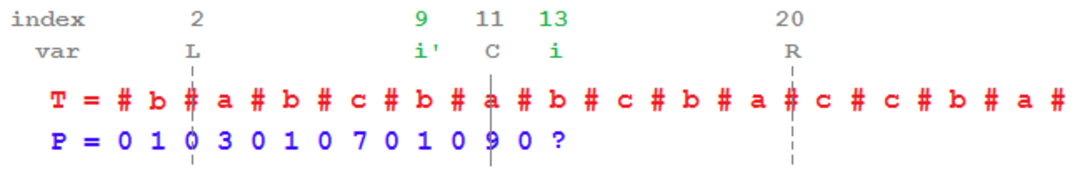
\includegraphics[width=0.95\textwidth]{Images/figLCLngstPlndrmcSubstring1}
\caption{Above image shows \ctt{T} transformed from
  \ctt{S=[babcbabcbaccba]}.  Assumed that you reached a state where table
  \ctt{P} is partially completed. The solid vertical line indicates the
  center (\ctt{C}) of the palindrome \ctt{abcbabcba}. The two dotted
  vertical line indicate its left (\ctt{L}) and right (\ctt{R}) edges
  respectively. You are at index $i$ and its mirrored index around \ctt{C}
  is \ctt{i'}. How would you calculate \ctt{P[i]} efficiently?}
%\label{figCXNX}
\end{figure}

Assume that we have arrived at index $i=13$, and we need to calculate
\ctt{P[13]} (indicated by the question mark \ctt{?}). We first look at its
mirrored index \ctt{i'} around the palindrome's center \ctt{C}, which is
index \ctt{i'=9}.

\begin{figure}
\centering
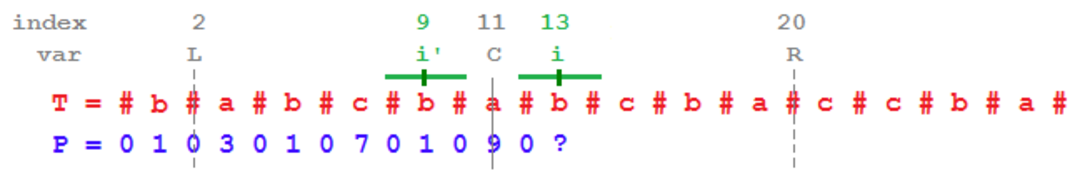
\includegraphics[width=0.95\textwidth]{Images/figLCLngstPlndrmcSubstring2}
\caption{The two green solid lines above indicate the covered region by the
  two palindromes centered at \ctt{i} and \ctt{i'}. We look at the mirrored
  index of \ctt{i} around \ctt{C}, which is index \ctt{i'}.
  \ctt{P[i']=P[9]=1}. It is clear that \ctt{P[i]} must also be \ctt{1}, due
  to the symmetric property of a palindrome around its center.}
%\label{figCXNX}
\end{figure}

As you can see above, it is very obvious that P[ i ] = P[ i' ] = 1, which
must be true due to the symmetric property around a palindrome's center. In
fact, all three elements after C follow the symmetric property (that is, P[
12 ] = P[ 10 ] = 0, P[ 13 ] = P[ 9 ] = 1, P[ 14 ] = P[ 8 ] = 0).

\begin{figure}
\centering
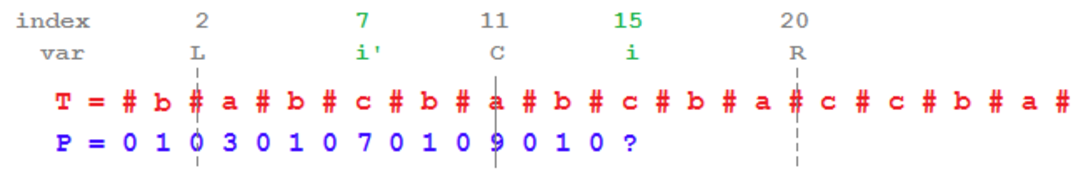
\includegraphics[width=0.95\textwidth]{Images/figLCLngstPlndrmcSubstring3}
\caption{Now we are at index i = 15, and its mirrored index around C is i' = 7. Is P[ 15 ] = P[ 7 ] = 7?}
%\label{figCXNX}
\end{figure}

Now we are at index i = 15. What's the value of P[ i ]? If we follow the
symmetric property, the value of P[ i ] should be the same as P[ i' ] = 7.
But this is wrong. If we expand around the center at T15, it forms the
palindrome “a\#b\#c\#b\#a”, which is actually shorter than what is indicated by
its symmetric counterpart. Why?


\begin{figure}
\centering
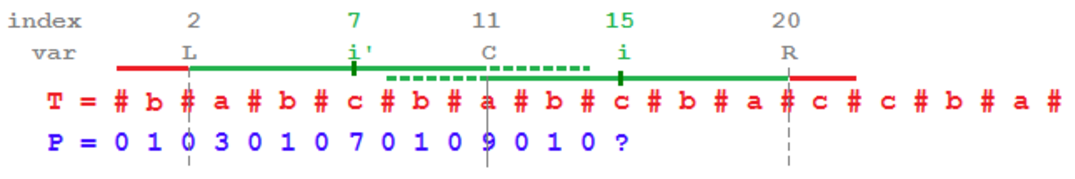
\includegraphics[width=0.95\textwidth]{Images/figLCLngstPlndrmcSubstring4}
Colored lines are overlaid around the center at index i and i'. Solid green lines show the region that must match for both sides due to symmetric property around C. Solid red lines show the region that might not match for both sides. Dotted green lines show the region that crosses over the center.
\caption{}
%\label{figCXNX}
\end{figure}

It is clear that the two substrings in the region indicated by the two solid
green lines must match exactly. Areas across the center (indicated by dotted
green lines) must also be symmetric. Notice carefully that P[ i ' ] is 7 and
it expands all the way across the left edge (L) of the palindrome (indicated
by the solid red lines), which does not fall under the symmetric property of
the palindrome anymore. All we know is P[ i ] geq 5, and to find the real
value of P[ i ] we have to do character matching by expanding past the right
edge (R). In this case, since P[ 21 ] neq P[ 1 ], we conclude that P[ i ] = 5.

Let's summarize the key part of this algorithm as below:

if P[ i' ] leq R - i,
then P[ i ] := P[ i' ]
else P[ i ] geq P[ i' ]. (Which we have to expand past the right edge (R) to find P[ i ].

See how elegant it is? If you are able to grasp the above summary fully, you
already obtained the essence of this algorithm, which is also the hardest
part.

The final part is to determine when should we move the position of C
together with R to the right, which is easy:

If the palindrome centered at i does expand past R, we update C to i, (the
center of this new palindrome), and extend R to the new palindrome's right
edge.

In each step, there are two possibilities. If P[ i ] leq R - i, we set P[ i ]
to P[ i' ] which takes exactly one step. Otherwise we attempt to change the
palindrome's center to i by expanding it starting at the right edge, R.
Extending R (the inner while loop) takes at most a total of N steps, and
positioning and testing each centers take a total of N steps too. Therefore,
this algorithm guarantees to finish in at most 2*N steps, giving a linear
time solution.



%%%%%%%%%%%%%%%%%%%%%%%%%%%%%%%%%%%%%%%%%%%%%%%%%%%%%%%%%%%%%%%%%%%%%%%%%%%%
%%%%%%%%%%%%%%%%%%%%%%%%%%%%%%%%%%%%%%%%%%%%%%%%%%%%%%%%%%%%%%%%%%%%%%%%%%%%
%%%%%%%%%%%%%%%%%%%%%%%%%%%%%%%%%%%%%%%%%%%%%%%%%%%%%%%%%%%%%%%%%%%%%%%%%%%%

\section{Longest Palindromic Substring | Set 1
  \label{secLPSStrGFGLngstPlndrmcSbstrngSet1}}

\url{https://www.geeksforgeeks.org/longest-palindrome-substring-set-1}

\textbf{Difficulty: 3.5}

\textbf{\rrgreen{Recommended: Please try your approach first, before moving
    on to the solution.}}

\RayNotesBegin

I understand already, moving onto Manacher's algorithm

\RayNotesEnd

\textbf{\rrgreen{Back to geeksforgeeks solution.}}





%%%%%%%%%%%%%%%%%%%%%%%%%%%%%%%%%%%%%%%%%%%%%%%%%%%%%%%%%%%%%%%%%%%%%%%%%%%%
%%%%%%%%%%%%%%%%%%%%%%%%%%%%%%%%%%%%%%%%%%%%%%%%%%%%%%%%%%%%%%%%%%%%%%%%%%%%
%%%%%%%%%%%%%%%%%%%%%%%%%%%%%%%%%%%%%%%%%%%%%%%%%%%%%%%%%%%%%%%%%%%%%%%%%%%%

\section{Longest Palindromic Substring | Set 2
  \label{secLPSStrGFGLngstPlndrmcSbstrngSet2}}

\url{https://www.geeksforgeeks.org/longest-palindromic-substring-set-2}

\textbf{Difficulty: 3.2}

\textbf{\rrgreen{Recommended: Please try your approach first, before moving
    on to the solution.}}

\RayNotesBegin

I understand already, moving onto Manacher's algorithm

\RayNotesEnd

\textbf{\rrgreen{Back to geeksforgeeks solution.}}




%%%%%%%%%%%%%%%%%%%%%%%%%%%%%%%%%%%%%%%%%%%%%%%%%%%%%%%%%%%%%%%%%%%%%%%%%%%%
%%%%%%%%%%%%%%%%%%%%%%%%%%%%%%%%%%%%%%%%%%%%%%%%%%%%%%%%%%%%%%%%%%%%%%%%%%%%
%%%%%%%%%%%%%%%%%%%%%%%%%%%%%%%%%%%%%%%%%%%%%%%%%%%%%%%%%%%%%%%%%%%%%%%%%%%%

\section{Manacher's Algorithm -- Linear Time Longest Palindromic Substring -- Part 1
  \label{secLPSStrGFGManacherPt1}}

\url{https://www.geeksforgeeks.org/manachers-algorithm-linear-time-longest-palindromic-substring-part-1}

\textbf{Difficulty: 3.7}

Given a string, find the longest substring which is palindrome.
\begin{itemize}[noitemsep,topsep=0pt]
\item if the given string is \ctt{forgeeksskeegfor}, the output should be
  \ctt{geeksskeeg}
\item if the given string is \ctt{abaaba}, the output should be \ctt{abaaba}
\item if the given string is \ctt{abababa}, the output should be
  \ctt{abababa}
\item if the given string is \ctt{abcbabcbabcba}, the output should be
  \ctt{abcbabcba}
\end{itemize}
We have already discussed Na\"ive $\comBigOh{n^3}$ and quadratic
$[\comBigOh{n^2}$ approaches at Set 1 and Set 2.

In this article, we will talk about Manacher's algorithm which finds Longest
Palindromic Substring in linear time.

One way (Set 2) to find a palindrome is to start from the center of the
string and compare characters in both directions one by one. If
corresponding characters on both sides (left and right of the center) match,
then they will make a palindrome.

Let's consider string \ctt{abababa}.

Here, center of the string is $4$th character (with index $3$) \ctt{b}. If
we match characters in left and right of the center, all characters match
and so string \ctt{abababa} is a palindrome.

\begin{figure}
\centering
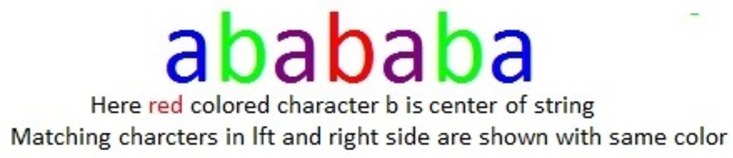
\includegraphics[width=0.5\textwidth]{Images/figGFGPalinManacher1}
%\caption[]{}
%\label{figCXNX}
\end{figure}

Here, center position is not only the actual string character position but it
could be the position between two characters also.  Consider string
\ctt{abaaba} of even length. This string is palindrome around the position
between $3$rd and $4$th characters \ctt{a} and \ctt{a} respectively.

\begin{figure}
\centering
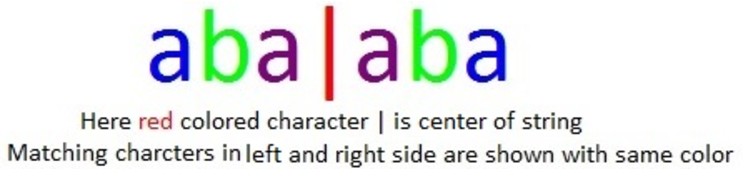
\includegraphics[width=0.5\textwidth]{Images/figGFGPalinManacher2}
%\caption[]{}
%\label{figCXNX}
\end{figure}

To find Longest Palindromic Substring of a string of length $N$, one way is
take each possible $2N+1$ centers (the $N$ character positions, $N-1$
between two character positions and $2$ positions at left and right ends),
do the character match in both left and right directions at each $2N+1$
centers and keep track of LPS. This approach takes $\comBigOh{N^2}$ time and
that's what we are doing in Set 2.

Let's consider two strings \ctt{abababa} and \ctt{abaaba} as shown below:

\begin{figure}
\centering
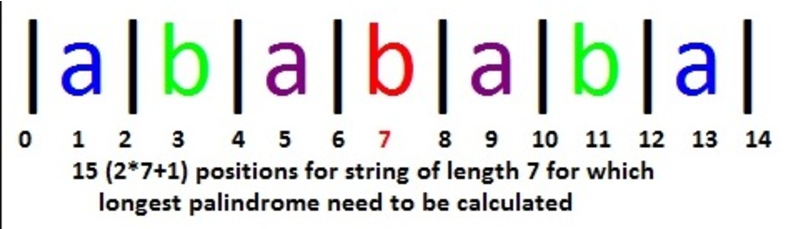
\includegraphics[width=0.5\textwidth]{Images/figGFGPalinManacher3}
%\caption[]{}
%\label{figCXNX}
\end{figure}

\begin{figure}
\centering
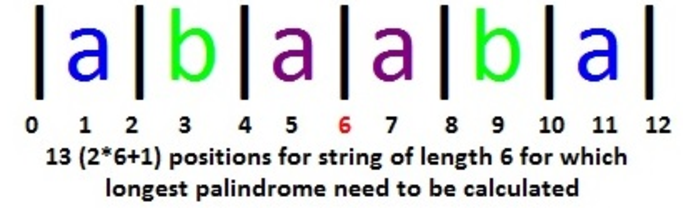
\includegraphics[width=0.5\textwidth]{Images/figGFGPalinManacher4}
%\caption[]{}
%\label{figCXNX}
\end{figure}

\rrblue{(Notice now if there is an odd number of chars, we add $N-1$ (even)
  $+2$ (even) for the end separators. This makes the total number of chars
  odd. If the number of chars is even, then we add an odd number of
  separators, again making the total number of chars even.)}

In these two strings, left and right side of the center positions (position
$7$ in $1$st string and position $6$ in $2$nd string) are symmetric. Why?
Because the whole string is palindrome around the center position.

If we need to calculate Longest Palindromic Substring at each $2N+1$
positions from left to right, then palindrome's symmetric property could
help to avoid some of the unnecessary computations (i.e. character
comparison). If there is a palindrome of some length $L$ centered at any
position $P$, then we may not need to compare all characters in left and
right side at position $P+1$. We already calculated LPS at positions before
$P$ and they can help to avoid \textbf{some} of the comparisons after
position $P$.

This use of information from previous positions at a later point of time
makes the Manacher's algorithm linear. In Set 2, there is no reuse of
previous information and so that is quadratic.

Manacher's algorithm is probably considered complex to understand, so here
we will discuss it in as detailed way as we can. Some of it's portions may
require multiple reading to understand it properly.

Let's look at string \ctt{abababa}. In 3rd figure above, 15 center positions
are shown. We need to calculate length of longest palindromic string at each
of these positions.
\begin{itemize}%[noitemsep,topsep=0pt]
\item At position $0$, there is no LPS at all (no character on left side to
  compare), so length of LPS will be $0$.
\item At position $1$, LPS is \ctt{a}, so length of LPS will be $1$.
\item At position $2$, there is no LPS at all (left and right characters
  \ctt{a} and \ctt{b} don't match), so length of LPS will be $0$.
\item At position $3$, LPS is \ctt{aba}, so length of LPS will be $3$.
\item At position $4$, there is no LPS at all (left and right characters
  \ctt{b} and \ctt{a} don't match), so length of LPS will be $0$.
\item At position $5$, LPS is \ctt{ababa}, so length of LPS will be $5$.
\end{itemize}
... and so on

We store all these palindromic lengths in an array, say $L$. Then string $S$
and LPS Length $L$ look like below:

\begin{figure}
\centering
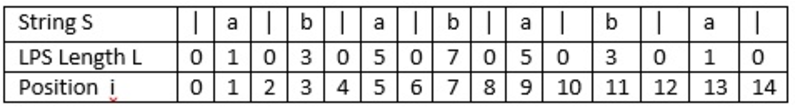
\includegraphics[width=0.7\textwidth]{Images/figGFGPalinManacher5}
%\caption[]{}
%\label{figCXNX}
\end{figure}

Similarly, LPS Length L of string \ctt{abaaba} will look like:

\begin{figure}
\centering
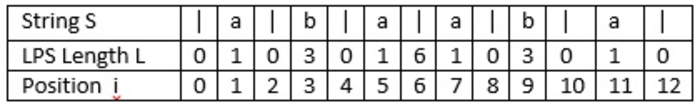
\includegraphics[width=0.7\textwidth]{Images/figGFGPalinManacher6}
%\caption[]{}
%\label{figCXNX}
\end{figure}

In LPS Array \ctt{L}:
\begin{itemize}%[noitemsep,topsep=0pt]
\item LPS length value at odd positions (the actual character positions)
  will be \textbf{odd} and \textbf{greater than or equal to 1} (1 will come
  from the center character itself if nothing else matches in left and right
  side of it) \rrblue{(It is odd because 1 will come from the center, and
    then we have characters on either side of the centre, total 1+even
    number of chars = odd number of chars)}
\item LPS length value at even positions (the positions between two
  characters, extreme left and right positions) will be even and greater
  than or equal to 0 (0 will come when there is no match in left and right
  side)
\end{itemize}
\begin{mdframed}[style=mdfNOTE]
\textbf{Position and index for the string are two different things here. For
  a given string $S$ of length $N$, indexes will be from $0$ to $N-1$ (total
  $N$ indexes) and positions will be from $0$ to $2N$ (total $2N+1$
  positions).}
\end{mdframed}

LPS length value can be interpreted in two ways, one in terms of index and
second in terms of position. LPS value $d$ at position $i$ ($L[i]=d$) tells
that:
\begin{itemize}%[noitemsep,topsep=0pt]
\item Substring from \textbf{position} $i-d$ to $i+d$ is a palindrome of
  length $d$ (in terms of position)
\item Substring from index $(i-d)/2$ to $[(i+d)/2-1]$ is a palindrome of
  length $d$ (in terms of index)
\end{itemize}
e.g. in string \ctt{abaaba}, \ctt{L[3]=3} means substring from position $0$
$(3-3)$ to $6$ $(3+3)$ is a palindrome which is \ctt{aba} of length $3$
\rrblue{(see red position numbers below)}, it also means that substring from
index $0$ $[(3-3)/2]$ to $2$ $[(3+3)/2-1]$ is a palindrome which is
\ctt{aba} of length $3$.

\begin{figure}
\centering
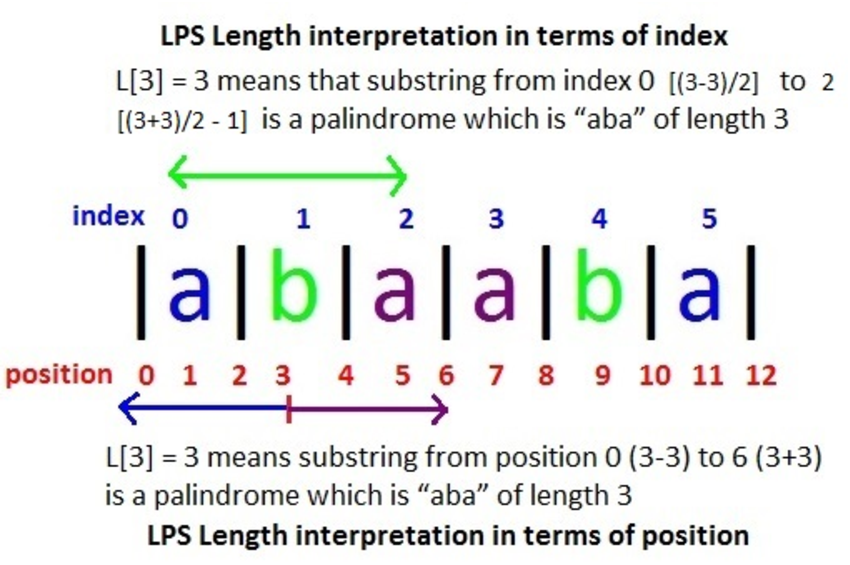
\includegraphics[width=0.7\textwidth]{Images/figGFGPalinManacher7}
%\caption[]{}
%\label{figCXNX}
\end{figure}

Now the main task is to compute LPS array efficiently. Once this array is
computed, LPS of string $S$ will be centered at position with maximum LPS
length value. We will see it in Part 2.

This article is contributed by Anurag Singh. Please write comments if you
find anything incorrect, or you want to share more information about the
topic discussed above

\RayNotesBegin

Okay, I give up for now. I just realised that this is in four parts.

\begin{itemize}%[noitemsep,topsep=0pt]
\item \url{todo}
\item \url{todo}
\item \url{todo}
\end{itemize}

\RayNotesEnd

%\textbf{\rrgreen{Recommended: Please try your approach first, before moving
%    on to the solution.}}
%
%\RayNotesBegin
%
%
%
%\RayNotesEnd
%
%\textbf{\rrgreen{Back to geeksforgeeks solution.}}



%%%%%%%%%%%%%%%%%%%%%%%%%%%%%%%%%%%%%%%%%%%%%%%%%%%%%%%%%%%%%%%%%%%%%%%%%%%%
%%%%%%%%%%%%%%%%%%%%%%%%%%%%%%%%%%%%%%%%%%%%%%%%%%%%%%%%%%%%%%%%%%%%%%%%%%%%
%%%%%%%%%%%%%%%%%%%%%%%%%%%%%%%%%%%%%%%%%%%%%%%%%%%%%%%%%%%%%%%%%%%%%%%%%%%%

\section{Manacher's Algorithm -- Linear Time Longest Palindromic Substring
  -- Part 2
  \label{secLPSStrGFGManacherPt2}}

\url{https://www.geeksforgeeks.org/manachers-algorithm-linear-time-longest-palindromic-substring-part-2}

\textbf{Difficulty: 4.4}

%In Manacher’s Algorithm – Part 1, we gone through some of the basics and LPS length array.
%Here we will see how to calculate LPS length array efficiently.
%
%To calculate LPS array efficiently, we need to understand how LPS length for any position may relate to LPS length value of any previous already calculated position.
%For string “abaaba”, we see following:
%
%\begin{figure}
%\centering
%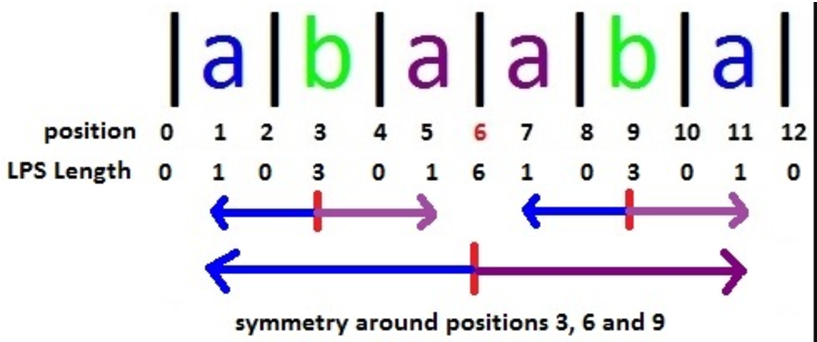
\includegraphics[width=0.7\textwidth]{Images/figGFGPalinManacher8}
%%\caption[]{}
%%\label{figCXNX}
%\end{figure}
%
%If we look around position 3:
%
%LPS length value at position 2 and position 4 are same
%LPS length value at position 1 and position 5 are same
%We calculate LPS length values from left to right starting from position 0, so we can see if we already know LPS length values at positions 1, 2 and 3 already then we may not need to calculate LPS length at positions 4 and 5 because they are equal to LPS length values at corresponding positions on left side of position 3.
%
%If we look around position 6:
%
%LPS length value at position 5 and position 7 are same
%LPS length value at position 4 and position 8 are same
%…………. and so on.
%If we already know LPS length values at positions 1, 2, 3, 4, 5 and 6 already then we may not need to calculate LPS length at positions 7, 8, 9, 10 and 11 because they are equal to LPS length values at corresponding positions on left side of position 6.
%
%For string “abababa”, we see following:
%
%\begin{figure}
%\centering
%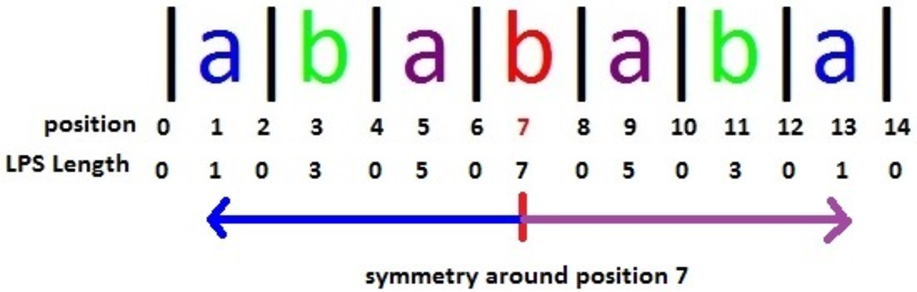
\includegraphics[width=0.7\textwidth]{Images/figGFGPalinManacher9}
%%\caption[]{}
%%\label{figCXNX}
%\end{figure}
%
%If we already know LPS length values at positions 1, 2, 3, 4, 5, 6 and 7 already then we may not need to calculate LPS length at positions 8, 9, 10, 11, 12 and 13 because they are equal to LPS length values at corresponding positions on left side of position 7.
%
%Can you see why LPS length values are symmetric around positions 3, 6, 9 in string “abaaba”? That’s because there is a palindromic substring around these positions. Same is the case in string “abababa” around position 7.
%Is it always true that LPS length values around at palindromic center position are always symmetric (same)?
%Answer is NO.
%Look at positions 3 and 11 in string “abababa”. Both positions have LPS length 3. Immediate left and right positions are symmetric (with value 0), but not the next one. Positions 1 and 5 (around position 3) are not symmetric. Similarly, positions 9 and 13 (around position 11) are not symmetric.
%
%At this point, we can see that if there is a palindrome in a string centered at some position, then LPS length values around the center position may or may not be symmetric depending on some situation. If we can identify the situation when left and right positions WILL BE SYMMETRIC around the center position, we NEED NOT calculate LPS length of the right position because it will be exactly same as LPS value of corresponding position on the left side which is already known. And this fact where we are avoiding LPS length computation at few positions makes Manacher’s Algorithm linear.
%
%In situations when left and right positions WILL NOT BE SYMMETRIC around the center position, we compare characters in left and right side to find palindrome, but here also algorithm tries to avoid certain no of comparisons. We will see all these scenarios soon.
%
%Let’s introduce few terms to proceed further:
%
%\begin{figure}
%\centering
%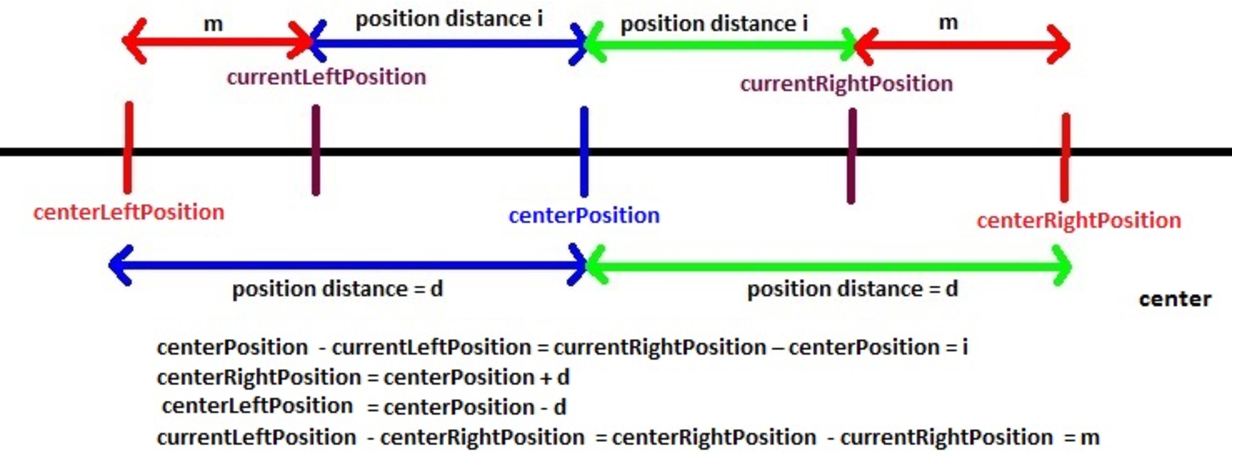
\includegraphics[width=0.7\textwidth]{Images/figGFGPalinManacher10}
%%\caption[]{}
%%\label{figCXNX}
%\end{figure}
%
%centerPosition – This is the position for which LPS length is calculated and let’s say LPS length at centerPosition is d (i.e. L[centerPosition] = d)
%centerRightPosition – This is the position which is right to the centerPosition and d position away from centerPosition (i.e. centerRightPosition = centerPosition + d)
%centerLeftPosition – This is the position which is left to the centerPosition and d position away from centerPosition (i.e. centerLeftPosition = centerPosition – d)
%currentRightPosition – This is the position which is right of the centerPosition for which LPS length is not yet known and has to be calculated
%currentLeftPosition – This is the position on the left side of centerPosition which corresponds to the currentRightPosition
%centerPosition – currentLeftPosition = currentRightPosition – centerPosition
%currentLeftPosition = 2* centerPosition – currentRightPosition
%i-left palindrome – The palindrome i positions left of centerPosition, i.e. at currentLeftPosition
%i-right palindrome – The palindrome i positions right of centerPosition, i.e. at currentRightPosition
%center palindrome – The palindrome at centerPosition
%When we are at centerPosition for which LPS length is known, then we also know LPS length of all positions smaller than centerPosition. Let’s say LPS length at centerPosition is d, i.e.
%L[centerPosition] = d
%
%It means that substring between positions “centerPosition-d” to “centerPosition+d” is a palindrom.
%Now we proceed further to calculate LPS length of positions greater than centerPosition.
%Let’s say we are at currentRightPosition ( > centerPosition) where we need to find LPS length.
%For this we look at LPS length of currentLeftPosition which is already calculated.
%
%If LPS length of currentLeftPosition is less than “centerRightPosition – currentRightPosition”, then LPS length of currentRightPosition will be equal to LPS length of currentLeftPosition. So
%L[currentRightPosition] = L[currentLeftPosition] if L[currentLeftPosition] < centerRightPosition – currentRightPosition. This is Case 1.
%
%Let’s consider below scenario for string “abababa”:
%
%\begin{figure}
%\centering
%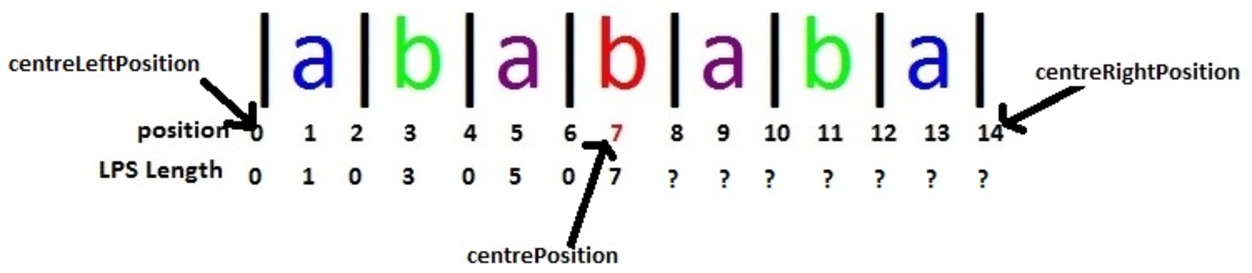
\includegraphics[width=0.7\textwidth]{Images/figGFGPalinManacher11}
%%\caption[]{}
%%\label{figCXNX}
%\end{figure}
%
%We have calculated LPS length up-to position 7 where L[7] = 7, if we consider position 7 as centerPosition, then centerLeftPosition will be 0 and centerRightPosition will be 14.
%Now we need to calculate LPS length of other positions on the right of centerPosition.
%
%For currentRightPosition = 8, currentLeftPosition is 6 and L[currentLeftPosition] = 0
%Also centerRightPosition – currentRightPosition = 14 – 8 = 6
%Case 1 applies here and so L[currentRightPosition] = L[8] = 0
%Case 1 applies to positions 10 and 12, so,
%L[10] = L[4] = 0
%L[12] = L[2] = 0
%
%If we look at position 9, then:
%currentRightPosition = 9
%currentLeftPosition = 2* centerPosition – currentRightPosition = 2*7 – 9 = 5
%centerRightPosition – currentRightPosition = 14 – 9 = 5
%
%Here L[currentLeftPosition] = centerRightPosition – currentRightPosition, so Case 1 doesn’t apply here. Also note that centerRightPosition is the extreme end position of the string. That means center palindrome is suffix of input string. In that case, L[currentRightPosition] = L[currentLeftPosition]. This is Case 2.
%
%Case 2 applies to positions 9, 11, 13 and 14, so:
%L[9] = L[5] = 5
%L[11] = L[3] = 3
%L[13] = L[1] = 1
%L[14] = L[0] = 0
%
%What is really happening in Case 1 and Case 2? This is just utilizing the palindromic symmetric property and without any character match, it is finding LPS length of new positions.
%
%When a bigger length palindrome contains a smaller length palindrome centered at left side of it’s own center, then based on symmetric property, there will be another same smaller palindrome centered on the right of bigger palindrome center. If left side smaller palindrome is not prefix of bigger palindrome, then Case 1 applies and if it is a prefix AND bigger palindrome is suffix of the input string itself, then Case 2 applies.
%
%The longest palindrome i places to the right of the current center (the i-right palindrome) is as long as the longest palindrome i places to the left of the current center (the i-left palindrome) if the i-left palindrome is completely contained in the longest palindrome around the current center (the center palindrome) and the i-left palindrome is not a prefix of the center palindrome (Case 1) or (i.e. when i-left palindrome is a prefix of center palindrome) if the center palindrome is a suffix of the entire string (Case 2).
%
%In Case 1 and Case 2, i-right palindrome can’t expand more than corresponding i-left palindrome (can you visualize why it can’t expand more?), and so LPS length of i-right palindrome is exactly same as LPS length of i-left palindrome.
%
%Here both i-left and i-right palindromes are completely contained in center palindrome (i.e. L[currentLeftPosition] <= centerRightPosition – currentRightPosition)
%Now if i-left palindrome is not a prefix of center palindrome (L[currentLeftPosition] < centerRightPosition – currentRightPosition), that means that i-left palindrome was not able to expand up-to position centerLeftPosition.
%
%If we look at following with centerPosition = 11, then
%
%\begin{figure}
%\centering
%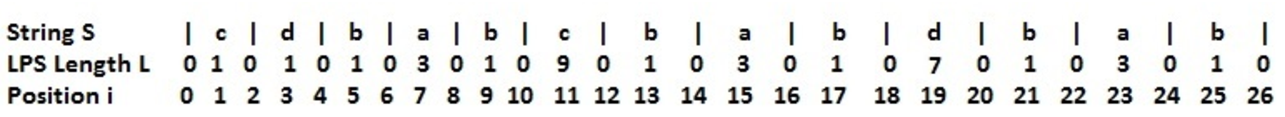
\includegraphics[width=0.7\textwidth]{Images/figGFGPalinManacher12}
%%\caption[]{}
%%\label{figCXNX}
%\end{figure}
%
%centerLeftPosition would be 11 – 9 = 2, and centerRightPosition would be 11 + 9 = 20
%If we take currentRightPosition = 15, it’s currentLeftPosition is 7. Case 1 applies here and so L[15] = 3. i-left palindrome at position 7 is “bab” which is completely contained in center palindrome at position 11 (which is “dbabcbabd”). We can see that i-right palindrome (at position 15) can’t expand more than i-left palindrome (at position 7).
%
%If there was a possibility of expansion, i-left palindrome could have expanded itself more already. But there is no such possibility as i-left palindrome is prefix of center palindrome. So due to symmetry property, i-right palindrome will be exactly same as i-left palindrome and it can’t expand more. This makes L[currentRightPosition] = L[currentLeftPosition] in Case 1.
%
%Now if we consider centerPosition = 19, then centerLeftPosition = 12 and centerRightPosition = 26
%If we take currentRightPosition = 23, it’s currentLeftPosition is 15. Case 2 applies here and so L[23] = 3. i-left palindrome at position 15 is “bab” which is completely contained in center palindrome at position 19 (which is “babdbab”). In Case 2, where i-left palindrome is prefix of center palindrome, i-right palindrome can’t expand more than length of i-left palindrome because center palindrome is suffix of input string so there are no more character left to compare and expand. This makes L[currentRightPosition] = L[currentLeftPosition] in Case 2.
%
%Case 1: L[currentRightPosition] = L[currentLeftPosition] applies when:
%
%i-left palindrome is completely contained in center palindrome
%i-left palindrome is NOT a prefix of center palindrome
%Both above conditions are satisfied when
%L[currentLeftPosition] < centerRightPosition – currentRightPosition
%
%Case 2: L[currentRightPosition] = L[currentLeftPosition] applies when:
%
%i-left palindrome is prefix of center palindrome (means completely contained also)
%center palindrome is suffix of input string
%Above conditions are satisfied when
%L[currentLeftPosition] = centerRightPosition – currentRightPosition (For 1st condition) AND
%centerRightPosition = 2*N where N is input string length N (For 2nd condition).
%
%Case 3: L[currentRightPosition] > = L[currentLeftPosition] applies when:
%
%i-left palindrome is prefix of center palindrome (and so i-left palindrome is completely contained in center palindrome)
%center palindrome is NOT suffix of input string
%Above conditions are satisfied when
%L[currentLeftPosition] = centerRightPosition – currentRightPosition (For 1st condition) AND
%centerRightPosition < 2*N where N is input string length N (For 2nd condition).
%In this case, there is a possibility of i-right palindrome expansion and so length of i-right palindrome is at least as long as length of i-left palindrome.
%
%Case 4: L[currentRightPosition] > = centerRightPosition – currentRightPosition applies when:
%
%i-left palindrome is NOT completely contained in center palindrome
%Above condition is satisfied when
%L[currentLeftPosition] > centerRightPosition – currentRightPosition
%In this case, length of i-right palindrome is at least as long (centerRightPosition – currentRightPosition) and there is a possibility of i-right palindrome expansion.
%
%In following figure,
%
%\begin{figure}
%\centering
%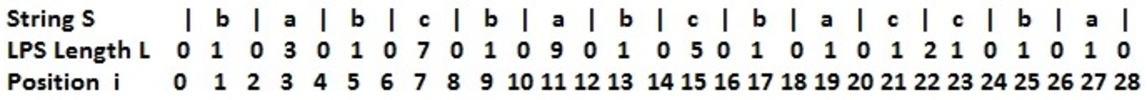
\includegraphics[width=0.7\textwidth]{Images/figGFGPalinManacher13}
%%\caption[]{}
%%\label{figCXNX}
%\end{figure}
%
%If we take center position 7, then Case 3 applies at currentRightPosition 11 because i-left palindrome at currentLeftPosition 3 is a prefix of center palindrome and i-right palindrome is not suffix of input string, so here L[11] = 9, which is greater than i-left palindrome length L[3] = 3. In the case, it is guaranteed that L[11] will be at least 3, and so in implementation, we 1st set L[11] = 3 and then we try to expand it by comparing characters in left and right side starting from distance 4 (As up-to distance 3, it is already known that characters will match).
%
%If we take center position 11, then Case 4 applies at currentRightPosition 15 because L[currentLeftPosition] = L[7] = 7 > centerRightPosition – currentRightPosition = 20 – 15 = 5. In the case, it is guaranteed that L[15] will be at least 5, and so in implementation, we 1st set L[15] = 5 and then we try to expand it by comparing characters in left and right side starting from distance 5 (As up-to distance 5, it is already known that characters will match).
%
%Now one point left to discuss is, when we work at one center position and compute LPS lengths for different rightPositions, how to know that what would be next center position. We change centerPosition to currentRightPosition if palindrome centered at currentRightPosition expands beyond centerRightPosition.
%
%Here we have seen four different cases on how LPS length of a position will depend on a previous position’s LPS length.
%In Part 3, we have discussed code implementation of it and also we have looked at these four cases in a different way and implement that too.
%
%This article is contributed by Anurag Singh. Please write comments if you find anything incorrect, or you want to share more information about the topic discussed above
%
%
%I give up, there's actually a part 3 and part four:
%
%https://www.geeksforgeeks.org/manachers-algorithm-linear-time-longest-palindromic-substring-part-3-2/
%
%https://www.geeksforgeeks.org/manachers-algorithm-linear-time-longest-palindromic-substring-part-4/
%


















\textbf{\rrgreen{Recommended: Please try your approach first, before moving
    on to the solution.}}

\RayNotesBegin



\RayNotesEnd

\textbf{\rrgreen{Back to geeksforgeeks solution.}}












\chapter[Leetcode Algorithms P1-P100]
{Leetcode Algorithms P1-P100
  \label{chLCP1P100}}
\chaptermark{LC P1-P100}



\section{11: Container With Most Water\label{secLCP11CntnrWthMstWtr}}

Given n non-negative integers $a_1$, $a_2$, $\ldots$, $a_n$, where each
represents a point at coordinate $(i,a_i)$. $n$ vertical lines are drawn
such that the two endpoints of line $i$ is at $(i,a_i)$ and $(i,0)$. Find
two lines, which together with $x$-axis forms a container, such that the
container contains the most water.

Note: You may not slant the container and $n$ is at least $2$.

\rrsepline{}

\rrheader{Approach \#1 Brute Force [Time Limit Exceeded]}

\noindent{}\textbf{Algorithm}\\
In this case, we will simply consider the area for every possible pair of
the lines and find out the maximum area out of those.
\begin{lstlisting}[style=raycppnewsnippet]
public class Solution {
  public int maxArea(int[] height) 
  {
    int maxarea = 0;
    for (int i = 0; i < height.length; i++)
      for (int j = i + 1; j < height.length; j++)
        maxarea = Math.max(maxarea, Math.min(height[i],
                                             height[j]) * (j - i));
    
    return maxarea;
  }
}
\end{lstlisting}

\noindent{}\textbf{Complexity Analysis}\\
\begin{itemize}%[noitemsep,topsep=0pt]
\item Time complexity: $\comBigOh{n^2}$. Calculating areas for all
  $\displaystyle \frac{n(n-1)}{2}$ height pairs.
\item Space complexity: $\comBigOh{1}$. Constant extra space used.
\end{itemize}

Note that we only have to consider $\frac{n(n-1)}{2}$ pairs (to calculate
the areas), since once we've calculated the area for $i$ with $j$, the area
for $j$ with $i$ is the same.  That is, they are symmetric.

\rrheader{Approach \#2 (Two Pointer Approach) [Accepted]}

\noindent{}\textbf{Algorithm}\\
The intuition behind this approach is that the area formed between the lines
will always be limited by the height of the shorter line. Further, the
farther the lines, the more will be the area obtained.

We take two pointers, one at the beginning and one at the end of the array
constituting the length of the lines. Further, we maintain a variable
\ctt{maxarea} to store the maximum area obtained till now. At every step, we
find out the area formed between them, update \ctt{maxarea} and move the
pointer pointing to the \textbf{shorter line} towards the other end by one
step.

The algorithm can be better understood by looking at the example below:
\begin{lstlisting}[style=raygeneric]
1 8 6 2 5 4 8 3 7
\end{lstlisting}

See the gif here: https://leetcode.com/problems/container-with-most-water/solution/

How this approach works?

Initially we consider the area constituting the exterior most lines. Now, to
maximize the area, we need to consider the area between the lines of larger
lengths. 

\textbf{If we try to move the pointer at the longer line inwards, we won't
gain any increase in area, since it is limited by the shorter line.}
\rrblue{(Think about it, since moving the longer line will reduce the length
  of the base, but the height is still limited by the shorter line.)}

\textbf{But moving the shorter line's pointer could turn out to be
  beneficial, as per the same argument, despite the reduction in the width.}
\rrblue{(Since we may read a line where the height more than offset the
  reduction in width.)} \emph{This is done since a relatively longer line
  obtained by moving the shorter line's pointer might overcome the reduction
  in area caused by the width reduction.}

For further clarification click
here\footnote{https://discuss.leetcode.com/topic/3462/yet-another-way-to-see-what-happens-in-the-o-n-algorithm}
and for the proof click here\footnote{https://discuss.leetcode.com/topic/503/anyone-who-has-a-o-n-algorithm/2}.

I shall cover both now.

\rrsepline{}

The $\comBigOh{n}$ solution with proof by contradiction doesn't look
intuitive enough to me. Before moving on, read the algorithm first if you
don't know it yet.

Here's another way to see what happens in a matrix representation:

Draw a matrix where the row is the first line, and the column is the second
line. For example, say $n=6$.

In the figures below, $x$ means we don't need to compute the volume for that
case: \textbf{(1)} On the diagonal, the two lines are overlapped;
\textbf{(2)} The lower left triangle area of the matrix is symmetric to the
upper right area.

We start by computing the volume at $(1,6)$, denoted by $o$. Now, if the
left line is shorter than the right line, then all the elements left to
$(1,6)$ on the first row have smaller volume \rrblue{(because in those, we
  keep the shorter one still $(i=1)$ but we move the longer one $(j=6)$,
  thus reducing the width)}, so we don't need to compute those cases
(crossed by $-{}-{}-$).
\begin{lstlisting}[style=raygeneric]
  1 2 3 4 5 6
1 x ------- o
2 x x
3 x x x 
4 x x x x
5 x x x x x
6 x x x x x x
\end{lstlisting}
Next we move the left line and compute $(2,6)$. Now if the right line is
shorter, all cases below $(2,6)$ are eliminated. \rrblue{(If the right line
  is shorter, then the same principal applies, there's no point moving the
  left line $i=2$ towards $j=6$, because we just reduce the width without
  being able to increase the max length of the two lines)}
\begin{lstlisting}[style=raygeneric]
  1 2 3 4 5 6
1 x ------- o
2 x x       o
3 x x x     |
4 x x x x   |
5 x x x x x |
6 x x x x x x
\end{lstlisting}
And no matter how this $o$ path goes, we end up only need to find the max
value on this path, which contains $n-1$ cases.
\begin{lstlisting}[style=raygeneric]
  1 2 3 4 5 6
1 x ------- o
2 x x - o o o
3 x x x o | |
4 x x x x | |
5 x x x x x |
6 x x x x x x
\end{lstlisting}
Hope this helps. I feel more comfortable seeing things this way.

Let's code this up.
























































\appendix
\counterwithin{figure}{chapter}

%\include{Contents/pt04Appndxs}
%\include{Contents/chAThOnDfntnRl}
%\include{Contents/chBVlCtgrs}
%\include{Contents/chCOvrldRsltn}
%\include{Contents/chDStndrdTypUtlts}
%\include{Contents/chECncpts}

%\chapter{Causality}
%
%\lipsum[1-15]

\backmatter

%%% BIBLIOGRAPHY
%%% -------------------------------------------------------------

% \bibliographystyle{utphysics}
% \bibliography{ref}

\defbibnote{myprenote}{Numbers in brackets following a reference give page numbers where the reference is cited.}
% Does what it says (using biblatex package)
\printbibliography[prenote=myprenote]
%\printbibliography

%\begingroup
%%\setstretch{0.9}
%\sloppy
%%\singlespacing
%\setlength\bibitemsep{1pt}
%\printbibliography
%\endgroup

\end{document}
